% This is an example of how to use the "npsthesis" document style for theses
% Modified for personal use by Fabrice Ardhuin, 2001/03/10
%
%  TO DO : add http://upload.wikimedia.org/wikipedia/commons/d/db/Munk_ICCE_1950_Fig1.svg  in ch1 

\documentclass[a4paper]{book}  % psfig for Encapsulated PostScript
%\usepackage{fullpage}
\addtolength{\oddsidemargin}{-0.4in} \addtolength{\evensidemargin}{-1.1in}
\addtolength{\textwidth}{1.5in} \addtolength{\topmargin}{-0.5in}
\addtolength{\textheight}{1.4in}
\usepackage[pdftex]{graphicx}
\usepackage{amsmath}
\usepackage{bm}
\pdfcompresslevel9
\usepackage[american]{babel}
% %\usepackage{upmath}
\usepackage[latin1]{inputenc}
%\usepackage[pdflatex]{graphics}
\usepackage{makeidx}
\usepackage{hyperref}
\usepackage{float}
\usepackage[section]{placeins}
 \usepackage{xcolor}
\hypersetup{
    colorlinks,
    linkcolor={red!50!black},
    citecolor={blue!50!black},
    urlcolor={blue!80!black}
}

%\usepackage[pdftex,plainpages=false]{hyperref}
\usepackage{natbib}
\setlength{\bibsep}{0em}

%\degree{Doctor of Philosophy In Oceanography}

% these macros save typing:
\newcommand{\beq}{\begin{equation}}
\newcommand{\beqa}{\begin{eqnarray}}
\newcommand{\eeq}{\end{equation}}
\newcommand{\eeqa}{\end{eqnarray}}
%
%\newcommand\p3{Part 3}
%\newcommand\p2{Part 2}
%\newcommand\p1{Part 1}

%   don't have right font for script R, so use:
\renewcommand{\Re}{{\cal R}}
\providecommand\boldsymbol[1]{\mbox{\boldmath $#1$}}
\providecommand\bnabla{\boldsymbol{\nabla}}
\providecommand\bcdot{\boldsymbol{\cdot}}
\providecommand\upi{\pi}
\newcommand\biS{\mathbf{S}}
\newcommand\cb{\mathbf{c}}
\newcommand\Cb{\mathbf{C}}
\newcommand\Mb{\mathbf{M}} 
\newcommand\dr{\mathrm{d}}
\newcommand\er{\mathrm{e}}
\newcommand\etb{\mathbf{\eta}}
\newcommand\ir{\mathrm{i}}
\newcommand\hu{\widehat{u}}
\newcommand\hv{\widehat{v}}
\newcommand\hw{\widehat{w}}
\newcommand\uL{\overline{u}^L}
\newcommand\wL{\overline{w}^L}
\newcommand\Eb{\mathbf{E}}
\newcommand\Sb{\mathbf{S}}
\newcommand\Ub{\mathbf{U}}
\newcommand\ub{\mathbf{u}}
\newcommand\xb{\mathbf{x}}
\newcommand\Kb{\mathbf{K}}
\newcommand\kb{\mathbf{k}}
\newcommand\kpb{\mathbf{k^{\prime}}}
\newcommand\lb{\mathbf{l}}
\newcommand\zerob{\mathbf{0}}
\newcommand\Deltab{\mathbf{\Delta}}
\newcommand\etal{\mbox{\textit{et al.}}}
\newcommand\etc{etc.\ }
\newcommand\eg{e.g.\ }
\newcommand\Real{\mathrm{Real}}
\newcommand\Frou{\mbox{\textit{Fr}}}  % Froude number
\newcommand\ttz{\ensuremath{\rightarrow 0}}
\newcommand\Ur{\mbox{\textit{Ur}}}  % Ursell number
\newcommand\Vb{\mathbf{V}}
\newcommand\zb{\overline{\zeta}}  
\newcommand\zL{\overline{\zeta}^L}

\def\sfbsL{\mathsfbi{L}}
\def\sfbsV{\mathsfbi{V}}
\def\sfbsD{\mathsfbi{D}}
\def\d{.}    % decimal mark

\newcommand{\boxedeqn}[1]{%
  \[\fbox{%
      \addtolength{\linewidth}{-2\fboxsep}%
      \addtolength{\linewidth}{-2\fboxrule}%
      \begin{minipage}{\linewidth}%
      \begin{equation}#1\end{equation}%
      \end{minipage}%
    }\]%
}


\begin{document}
\title{{\Huge Ocean waves in geosciences }
{\Large \\  parts 1 and 2: general wave topics from deep to shallow water}
 \vspace{3.0cm}\\
   \centerline{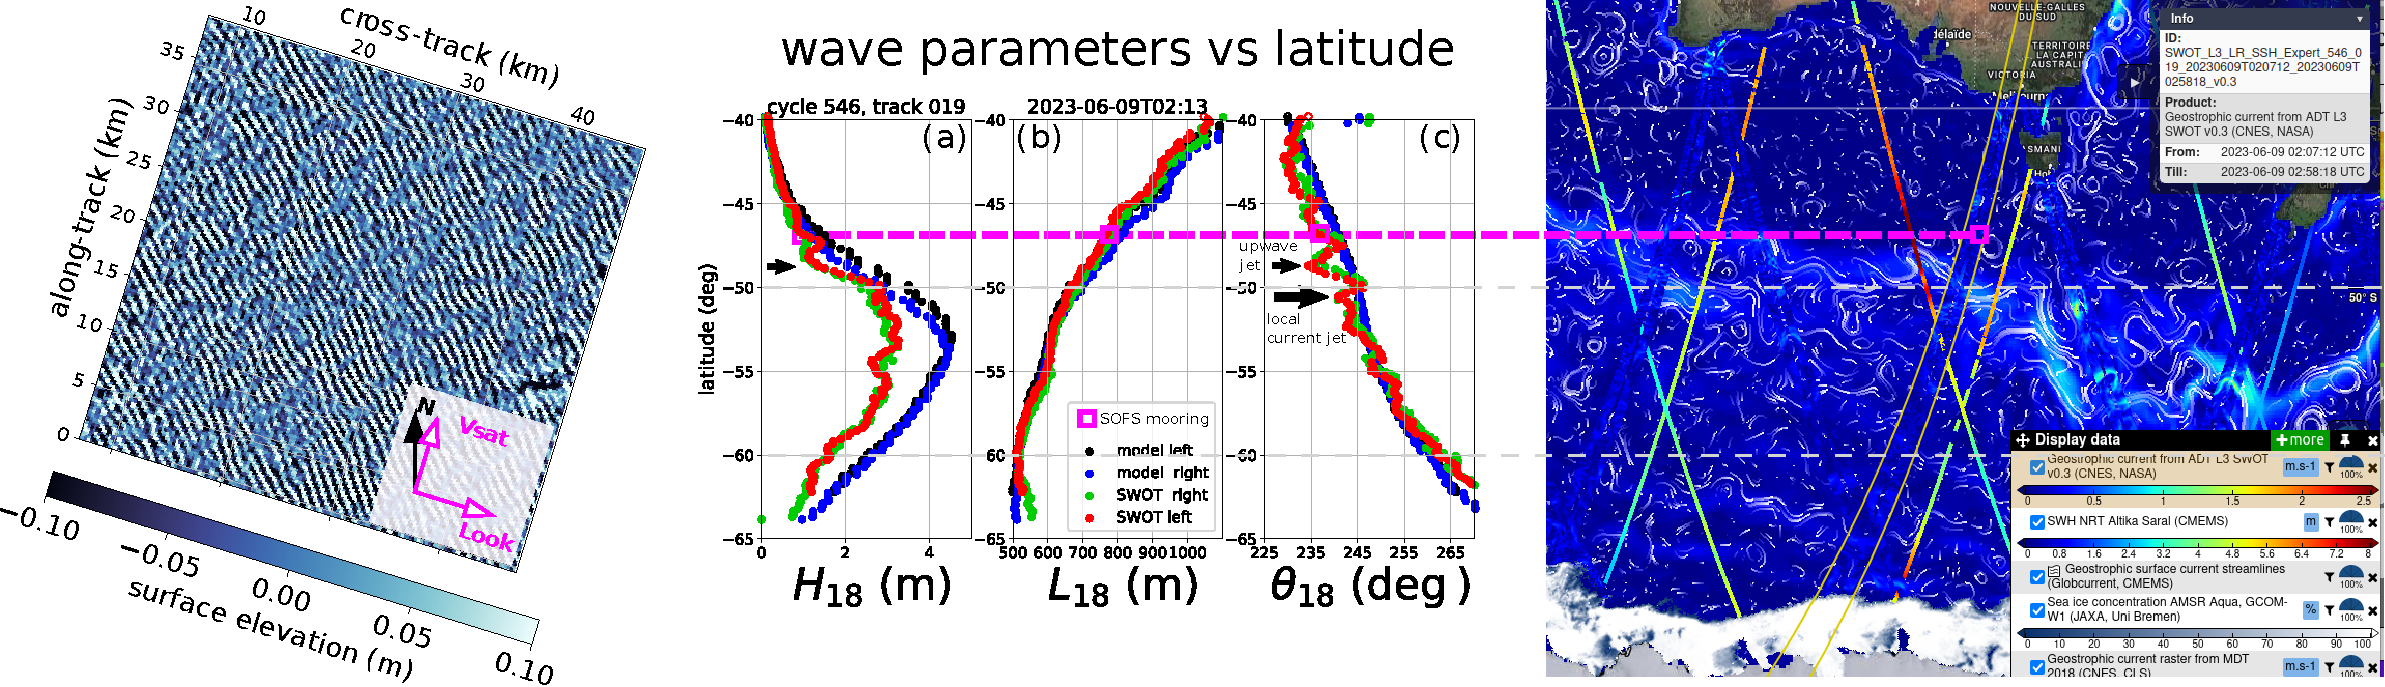
\includegraphics[width=\textwidth]{cover.pdf}}}
%%%%%%%%%%%%% figure
%\begin{figure}
%\centerline{\includegraphics[width=0.7\textwidth]{couv_cours.eps}}
%\vspace{3.64in}
%\end{figure}
%%%%%%%%%%%%% end of figure
\author{Fabrice Ardhuin, \\
\vspace{0.5cm}\\
Laboratoire d'Oc{\'e}anographie Physique et Spatiale, Brest,
France \\
\vspace{0.5cm}\\
doi:  10.13140/RG.2.2.16019.78888/11 ,  \url{https://github.com/ardhuin/waves_in_geosciences} \\
\vspace{1.5cm}\\
} \maketitle
\clearpage
On the cover: swell waves from extratropical storm Rosemary resolved by SWOT at the location of the SOFS mooring, South of Australia, along track 19, on 9 June 2023. The right panel uses the Ocean Virtual Laboratory developed by Oceandatalab to provide context for these wave observations: SWOT-derived currents, and other satellite altimeter wave heights (\url{https://odl.bzh/WjEKPhZa}). Such long waves waves are generated by the winds of the most powerful storm, and propagate across ocean basins where they are are also influenced by currents and sea ice. More details on this example in Ardhuin et al. (2024). 
 \cleardoublepage
\pagenumbering{roman}

\setcounter{page}{3}

\tableofcontents
\cleardoublepage


%\mainmatter
\setcounter{chapter}{0}

\pagenumbering{arabic}
\chapter*{Foreword}\label{foreword}
There are countless scholarly articles and books about ocean waves, with many different points of view, going from 
mathematical treatises to naval architecture. Among these we can single out the excellent textbooks by 
\cite{Kinsman1965}, \cite{Dean&Dalrymple1991},  
and \cite{Holthuijsen2007}, the engineering manual from the \cite{USACE2002}, and many excellent scientific 
monographs by \cite{Phillips1977}, \cite{Dingemans1997a}, \cite{Young1999}, \cite{Lavrenov2003}, \cite{Janssen2004}, \cite{Lannes2013} ...  

So why another one? 

First of all, scientific developments never stop, making these previous works not obsolete but less up to date 
and complete. This will happen with the present book, even if I am trying to update it on a regular basis. The parts 1 and 2 
and the associated teaching material (jupyter notebooks ...)  is designed to be at the level of Master students in oceanography. 

Second, and more important, all these books, except possibly the jewel by \cite{Phillips1977} have a rather narrow 
scope, and do not cover aspects for which no recent monograph exist. I particularly think about microseisms, infragravity waves or 
measurement techniques including satellite remote sensing. Some of these topics are only treated in part 3.

Working with coastal engineers, geomorphologists and seismologists, has motivated me to bring to 
the forefront those results that are often obscure or very hard to follow. My point of view is that 
ocean waves play a very particular role in the Earth System, both as an important element of air-sea or land-ocean exchanges, and also as a deforming mirror that 
modifies our measurements of ocean properties using remote sensing and even in situ techniques. As a result, much insight and cross-fertilization 
can come from the integration of many geoscientifc fields, from 
microseisms to remote sensing, as well as applied disciplines such as marine meteorology or coastal and ocean engineering.
At the very least, these different disciplines are providing new data, tools, and different points of view that complement each other 
in constraining  our physical understanding of wave processes, and the parameterizations used in numerical models or remote sensing algorithms. 

On these topics, I have tried to be clear without compromising the 
accuracy of the results, but this is a very difficult balance. If you find it unclear, do not hesitate to contact me
and I will try again to clarify in the next revision. I shall finish with a final warning:  my selection of topics is clearly biased to my own tastes and 
interests, which are clearly favouring geosciences versus engineering. It does not mean that the topics ignored here are not important. 
For example, a good discussion of 
extreme waves and sea state analysis would be much more useful for all engineers 
than our development on three-dimensional wave-current interactions. For this you may go to section 4.3 of \cite{Holthuijsen2007} or, with more details, to \cite{Boccotti2000}.
I hope that the present book will be a good combination 
of useful and interesting topics. \\

\vspace{0.5cm}
The document is organized in two parts, one relevant to waves in deep water, another providing additional 
information on coastal and shallow water aspects, and both are complemented by a separate book, which contains a third part that goes into some details that are probably not relevant for 
most readers in particular Master students. This book is designed to make it easier to read in electronic form, including hypertext links within the document 
and towards outside sources, such as the cited references. It is designed as a teaching material for the wave-related Master courses 
at University of Brest and ENSTA-Paris Tech. Because the present document is trying to follow the latest 
advances in research -- and my imperfect understanding of these. The permanent evolution unfortunately leads to the presence of errors, more so in part III. 
I thank 
Nicolas Rascle, Nadine Paugam, Cl�ment Gandon, Nobuhiro Suzuki, Sophia Brumer, Marine De Carlo and Oyvind Brevik for many corrections, Jean-Fran{\c c}ois Filipot for contributions and help in translating chapter 3, and 
Philippe Bonneton for discussions and help on the structure and contents of chapter \ref{ch_surf}.  
%This version is still not finished and some (old) parts in chapter 22-26 are still in French and will be translated in the coming months. OK, months may be years as I've been writing this for about ten years, but I'm not giving up hope.
I thank you in advance for finding any dubious or strange contents, or broken links.

\part{Waves in deep water} 
\cleardoublepage
\chapter{Introduction}\label{ch1}
\section{Waves in geosciences}
From the ripples on a water puddle to large breaking waves on the beach, we have all seen waves. 
They can be familiar or threatening, possibly deadly for seasoned fishermen or yachtsmen 
\citep[e. g. ][]{Pierson1972,Greenslade2001b}. Waves can exert huge forces: just try to stand up in the surf,
in front of a two-meter tall wave that breaks. And two meters is a far cry from the maximum recorded wave height at sea, towering
32~m above the following crest \citep{Liu&al.2008b}. The most severe \textit{sea state}, estimated from satellite radar altimetry, had a significant 
wave height of 18.5~m \citep{Hanafin&al.2012,DeCarlo&Ardhuin2024}, which, as we shall see in this chapter, 
means that some wave heights probably exceeded 35~m. Surfing contests have also focused on some specific coastal areas where waves are strongly amplified and produce waves of 30~m height or more, such as in Nazare, Portugal.



%%%%%%%%%%%%%%%%%%%%%%%%%%%%%%%%%%%%%%%%%%%%%%%%%%%%%%%%%%%%%%%%%%%%%%
\begin{figure}[htb]
\centerline{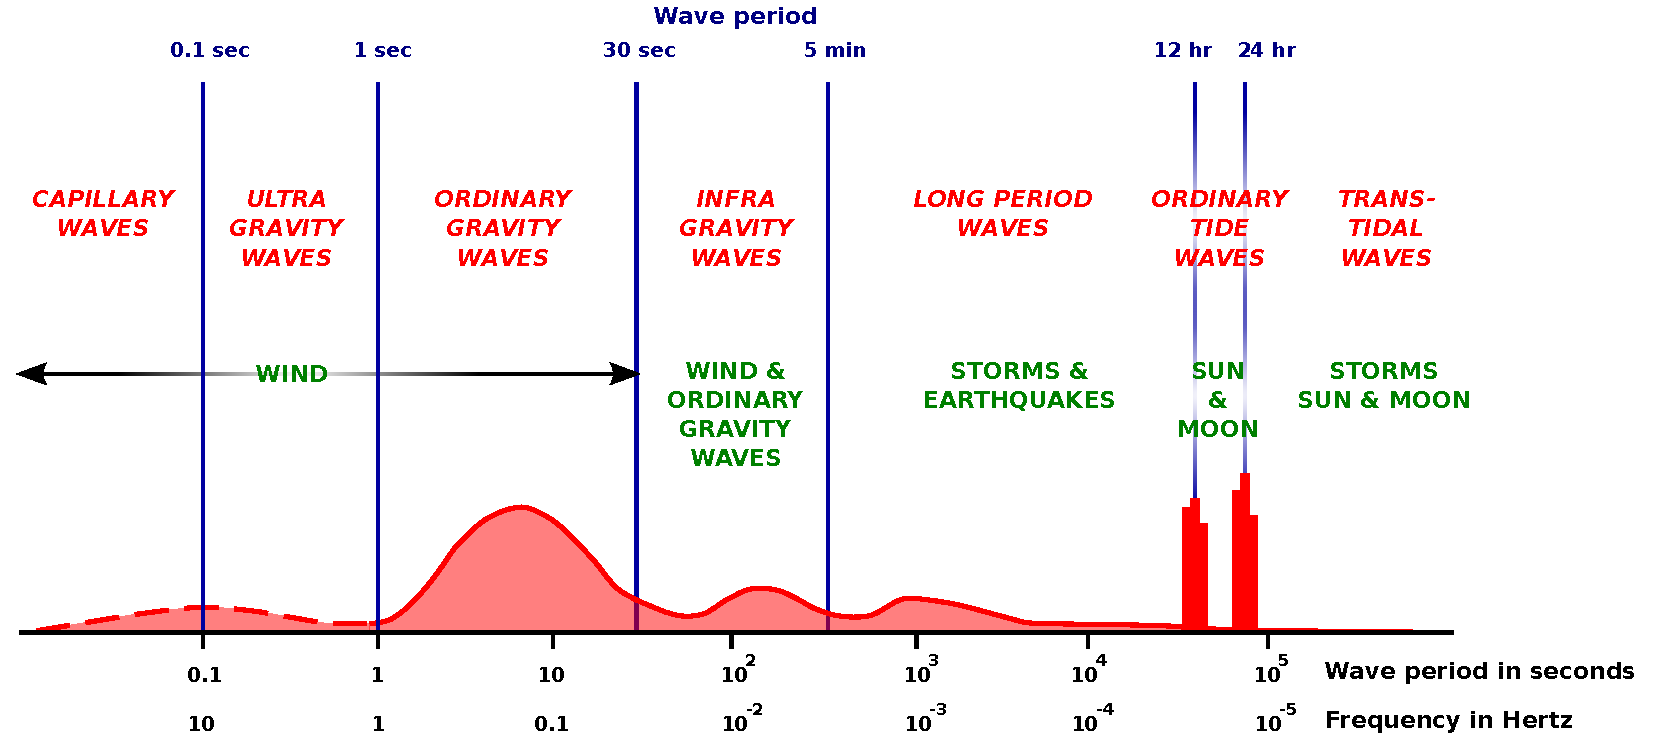
\includegraphics[width=\textwidth]{FIGS_CH_INTRO/Munk_ICCE_1950_Fig1.pdf}}
%\vspace{3.64in}
  \caption{Classification of ocean surface waves with usual names in red, as a function of wave periods (x-axis), with dominant forcing mechanisms in green. Adapted from \cite{Munk1950}.}
\label{fig:Munk1950}
\end{figure}
%%%%%%%%%%%%%%%%%%%%%%%%%%%%%%%%%%%%%%%%%%%%%%%%%%%%%%%%%%%%%%%%%%%%%%%%%
To be more precise, we need now to introduce some classification of the different wave motions. A simple classification, as proposed by 
\cite{Munk1950} and shown in figure \ref{fig:Munk1950}, is based on the typical time scales of between the passing of two crests. We shall call this time scale the wave period and denote it with the symbol $T$, even though the motion does not repeat itself exactly and is not mathematically speaking periodic. 

Figure \ref{fig:Munk1950} has boundaries between capillary waves, ultra gravity waves, ordinary gravity waves, infragravity waves and longer period waves (including tides) at periods of 0.1, 1, 30, and 300~s. Most of this book will focus on "ordinary gravity waves" with periods 1 to 30~s. As a physicist by training, I've never liked classifications with dimensional quantities that are often used in natural sciences: some of these distinctions are practically useful but they can be misleading.  Indeed, in some circumstances I would like to call "infragravity waves" some waves of periods around 10~s because they are generated by the same process as the "usual infragravity waves" with a period of 100~s. 

This period classification is closely related to a physical classification that distinguishes 
between the different  "restoring forces" which pulls back the surface towards a flat state, and the different generation processes for these waves. 
The two main restoring forces that we will consider are  \textbf{surface tension}, and \textbf{gravity}. Surface tension is mostly relevant for wave periods under 0.1~s, and will not be discussed much in the present book.

Once the restoring force is known, the next important things for any wave phenomenon are their
\begin{itemize}
          \item \textbf{generation},
          \item \textbf{propagation} 
          \item and \textbf{dissipation}.
         \end{itemize}
The goal of the present book is to describe and make understandable these 
three aspects, both qualitatively and quantitatively. 
This quantitative understanding allows an accurate forecast of local wave statistical properties, which we will 
call the sea state, as well as fluxes of energy and momentum between the atmosphere, ocean, sea ice, and solid Earth. 


In this book, we will restrict ourselves to waves which are more or less directly generated by the wind, leaving out 
tsunamis or ship wakes. But before leaving them out, let's say a few words about tsunamis. Tsunami propagation and dissipation properties 
are the same as the wind-waves described here, but whats sets them apart from wind-waves is their very large wavelength, 
which cannot be generated by wind in the same way as the usual wind-waves. Hence their generation mechanisms are specific, namely earthquakes, 
landslides, and meteorite 
impacts, which are all important but rare events, leading to very different statistical properties compared to the waves continuously 
generated by the wind. Another slightly more common source of meteo-tsunamis are abrupt changes in wind properties. 
All these generation events are transient, and typically cause a depression or bump of the sea surface that appears very fast but on a very 
large scale. This depression or bump then radiates a train of waves, with a period of the order of 10 minutes that is given by the size 
of the initial surface perturbation. These waves are strongly amplified in shallow water. The first perturbation to arrive on land can be a trough. 
If you see the sea retreating rapidly, this is it ... do not rush out to pick up crabs, but instead run to high ground, as a big crest will 
likely follow and flood what was the dry land. 

Instead of these transient wave trains, wind-generated waves are incessant and irregular.
The  time between the passing of two crests, which we define as the period $T$,  is typically less than 30~s. This limit is related 
to wind speeds, as explained in chapter \ref{ch_sourceterms}. 
These wind-waves also give rise to infra-gravity waves of periods 10~s to 10~minutes. For all these motions 
the average distance between two crests, which we shall call the mean wavelength $L_m$, increases with the mean period $T_m$. 
This wavelength goes from a few millimeters to about 1.2~km \citep{Ardhuin&al.2024}. For wave shorter than a few centimeters, the effect of surface 
tension must be taken into account, and these short waves are called gravity-capillary waves, and capillary waves when gravity can be neglected. 

Indeed, the \textbf{propagation} properties of waves is related to the balance of forces near the air-sea interface. If gravity or surface tension is the dominant force then the propagation is different.
Gravity fights against surface slopes, setting up a pressure gradient that tends to reduce the sea level slope and is the main force 
for large wavelengths. Surface tension, instead, fights against surface curvature:
it arises from the difference in thermodynamic properties of the interface between the two fluids, that are air and water. 
This difference gives an energy to their interface, which is proportional to the area of the interface: the more curved the surface the 
larger the surface energy. This surface energy is, for capillary waves, the equivalent of the gravitational potential energy. This force explains 
why water droplets are spherical: the sphere is the shape that minimizes the area (hence the energy) for a given volume. 
This surface tension also explains why short breaking waves are not energetic enough to generate bubbles and foam at the sea surface. 
The presence of a continuous layer of ice can also act like an elastic layer with an effect similar to surface tension. In this case
even long waves can be influenced by the elasticity of the ice layer, this influence depends on the ice thickness \citep[e.g.][]{Squire&al.1995}. 
Because curvature is the second derivative of the surface elevation, surface tension effects are much stronger than gravity for small scales. 

Whether gravity or surface tension is the main restoring force, the work of these forces produces a motion with an associated kinetic energy. 
The oscillations of the air-sea interface are thus maintained by an exchange between potential and kinetic energy, 
until this energy is \textbf{dissipated}. Our waves are thus surface gravity waves, gravity-capillary or capillary waves for the shortest. 

In the family of gravity waves, at the other extreme towards the large scales, the slow oscillations on time scales of several hours to several days 
are also influenced by 
the Coriolis force, caused by the rotation of the Earth, and the waves become inertial-gravity waves, also known as Kelvin and Poincar{\'e}
waves. The main \textbf{generation} forces for these are the wind and the difference in the gravitational pull exerted by the Moon and Sun on the 
center and the surface of the Earth. Kelvin waves share many properties of gravity waves.

%%%%%%%%%%%%%%%%%%%%%%%%%%%%%%%%%%%%%%%%%%%%%%%%%%%%%%%%%%%%%%%%%%%%%%
\begin{figure}
\centerline{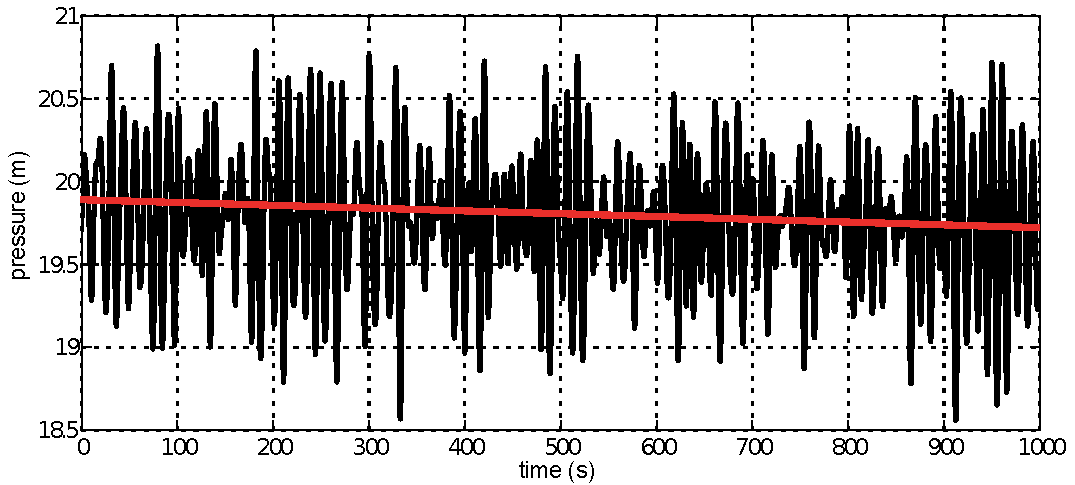
\includegraphics[width=\textwidth]{FIGS_CH_INTRO/p_at_berth1_en.pdf}}
%\vspace{3.64in}
  \caption{Example of the evolution of the bottom pressure in about 20~m of water 
 in Bertheaume bay, France, on January 31, 2004.}{The pressure in Pascals was converted here to an equivalent water height in meters
by dividing the absolute pressure 
recorded by a Nortek Vector %Seabird 26 
instrument, by the product $\rho_w g$ of water density $\rho_w \simeq 1026$kg/m$^3$, 
and gravity $g\simeq 9.81$m/s$^2$, after subtracting the atmospheric pressure recorded nearby, $p_a \simeq 10^5$Pa.  The 
fast oscillation caused by a swell of significant wave height $H_s=2.85$~m is superimposed on the tide 
that is gently falling, about 20~cm in 20~minutes, as shown by the red line.}
\label{pexemple}
\end{figure}
%%%%%%%%%%%%%%%%%%%%%%%%%%%%%%%%%%%%%%%%%%%%%%%%%%%%%%%%%%%%%%%%%%%%%%%%%

In practice, all these waves co-exist. Fortunately, it is often easy to sort them out and study them separately. 
Wind-waves and tides have very different periods and wavelengths, as illustrated by figure 
\ref{pexemple}. There is no such clear separation between capillary and gravity waves, except at low wind speeds 
when there is clear gap in the wave spectrum around the wavelength of 1.7~cm. For waves longer than 20~cm, 
we will ignore the effect of the surface tension which will greatly simplify our calculations. 
However, surface tension should not be ignored in general, in particular when considering 
wave dissipation by breaking and the effects of small scale surface roughness, both important for air-sea fluxes and remote sensing 
of the ocean surface.

The \textbf{propagation} of waves are generally well known thanks to the works of Laplace, Poisson, Stokes, Airy, Rayleigh and Boussinesq in 
the 18th and 19th centuries, with many later refinements. For a historical perspective, you may read the works of  \cite{Darrigol2003} and \cite{Craik2004}, and specific problems and questions are still open. The questions of  \textbf{generation} and \textbf{dissipation} are very active
research topics, with a fundamental problem posed by the multi-scale nature of real ocean waves: how short waves influence long waves and vice versa is 
very difficult to measure and analyze. Because of the strong demand for results, successful forecasting methods have been developed on more or less empirical grounds. 
Modern wave forecasting started with swell forecasts
for Morocco, in the 1920s \citep{Gain1918,Montagne1922}. This approach was generalized by 
\cite{Sverdrup&Munk1947} who considered the full life cycle of waves, from generation by the wind to dissipation 
in the middle of the ocean and on beaches. This latter work was 
motivated by the planning of the allied amphibious operation Torch in Morocco in 1942, which led to a method later applied to Normandy 
and many Pacific islands \citep{Bates1949}. Their British colleagues, forming the W group at the Admiralty, included Deacon, Darbyshire, Barber, Ursell and Longuet-Higgins  
who developed similar methods and introduced the spectral analysis of waves in 1945 \citep{Ursell1999}, paving the way for 
today's numerical wave models. The first numerical spectral wave model was developed by \cite{Gelci&al.1957}, the group that continued the Morocco wave forecasting effort in Casablanca.


Knowing and predicting the properties of waves is necessary for sea-going operations, the design of any marine structure such as 
a jetty, an offshore platform or a ship. Because waves are generated by the wind, there is an only tradition of telling the wind speed from the geometry of the waves, this is widely known as the Beaufort scale, reproduced in Table \ref{table_Beaufort} from \cite{Alcock&Morgan1978}. 

%%%%%%%%%%%%%%%%%%%%%%%%%%%%%%%%%%%%%%%%%%%%%%%%%%%%%%%%%%%%%%%%%%%%%%%%%%%%
\begin{table}
  \centering
  \begin{tabular}{|c|c|c|l|}
\hline
 Beaufort & descriptive     & wind speed  & specification for observation (open sea)  \\
 number   & term            &  (m/s)      &   \\
\hline
0               & Calm             &  0-1               & Sea like a mirror          \\
1               & Light air        &  1.5-2.5           & Ripples with the appearance of scales are formed \\
                &                  &                    & but without foam crests \\
2		& Light breeze     & 3 --4 		& Small wavelets still short but more pronounced; \\
                &                  &                    & crests have a glassy appearance and do not break \\
3               & Gentle breeze    & 4.5 --6            &  Large wavelets; crests begin to break;  foam of  \\
                &                  &                    & glassy appearance, perhaps scattered white horses \\
4		& Moderate breeze  & 6.5--8             &  Small waves becoming longer, fairly frequent white horses \\
5               & Fresh breeze     & 8.5-10.5           & Moderate waves, taking a more pronounced long form; \\
                &                  &                    & many white horses are formed (chance of some spray) \\
6               & Strong breeze    & 11--13.5           & Large waves begin to form; the white foam crests \\
                &                  &                    & are more extensive everywhere  (probably some spray)\\
7               &    Near gale     & 24--16.5           & Sea heaps up and white foam from breaking waves begins \\
                &                  &                    & to be blown in streaks along the direction of the wind \\
8               & Gale             & 17--20             & Moderately high waves of greater length; edges of crests \\
                &                 &                     & begin to break into the spindrift; the foam is blown in  \\
                &                &                    &  well-marked streaks along the direction of the wind  \\
9               & Strong gale     & 20.5--23.5         & High waves; dense streaks of foam along the direction of \\
                &                 &                    & the wind; crests of waves begin to topple, \\
                &                 &                    &tumble and roll over'; spray may affect visibility  \\
10              & Storm            & 24-27.5            & Very high waves with long overhanging crests; \\
                &                   &                  & the resulting foam, in great patches, is blown in dense \\
                &                  &                 & white streaks along the direction of the wind; on the whole \\
                &                  &                  & the surface of the sea takes on a white appearance; \\
                &                  &                  & the tumbling of the sea becomes heavy and shock-like; \\
                &                  &                  & visibility affected\\
11              & Violent storm    & 28--31.5           & Exceptionally high waves (small and medium-sized ships\\
                &                  &                    & might be for a time lost to view behind the waves); \\
                &                  &                    & the sea is completely covered with long white patches of \\
                &                  &                    & foam lying along the  direction of the wind; everywhere \\
                &                  &                    & the edges of the wave crests are blown into froth; \\
                &                  &                    &  visibility affected \\
12              & Hurricane        & 32 and over        &  The air is filled with foam and spray; sea completely \\
                &                  &                   &  white with driving spray; visibility very seriously affected  \\ 
\hline
\end{tabular}
\caption{The Beaufort scale for wind speed reproduced from \cite{Alcock&Morgan1978}. \label{table_Beaufort}}
\end{table}
%%%%%%%%%%%%%%%%%%%%%%%%%%%%%%%%%%%%%%%%%%%%%%%%%%%%%%%%%%%%%%%%%%%%%%%%%%%%

 Using the geometry of the waves and/or the properties of foam on the surface is still very much how we measure winds from satellite data, using scatterometers that measure the power of the radar echoes from the sea surface, or radiometers that measure the brightness temperature of the ocean surface. The relation between wind speed and those measurements
  is not unique because the waves may be at different stages of development. There is also a Beaufort scale for wave heights given in table \ref{table_seastate}, and clearly there is no one to one relationship between winds and waves. 


%%%%%%%%%%%%%%%%%%%%%%%%%%%%%%%%%%%%%%%%%%%%%%%%%%%%%%%%%%%%%%%%%%%%%%%%%%%%
\begin{table}
  \centering
  \begin{tabular}{|c|c|c|c|}
\hline
    \multicolumn{3}{|c|}{Wind sea} \\
 \hline
S code & descriptive term & wind sea wave height in meters (well developed)  \\
0 & calm (glassy)         & 0 \\
1 & calm (rippled)        & 0--0.1\\
2 & smooth (wavelets)     & 0.1--0.5 \\
3 & Slight                & 0.5--1.25  \\
4 & Moderate              & 1.25 --2.5  \\
5 & Rough                 & 2.5--4 \\
6 & Very Rough            & 4--6  \\
7 & High                  & 6--9 \\
8 & Very high             & 9--14  \\
9 & Phenomenal            & Over 14  \\
\hline
\end{tabular}
\caption{The Beaufort scale for sea states: source World Meteorological Organization, table 3700 \label{table_beaufort}}
\label{table_seastate}
\end{table}
%%%%%%%%%%%%%%%%%%%%%%%%%%%%%%%%%%%%%%%%%%%%%%%%%%%%%%%%%%%%%%%%%%%%%%%%%%%%


Waves modify the fluxes of momentum between the ocean and atmosphere and thus influence more or less directly the oceanic and 
atmospheric circulation. Waves are also an important agent in the pick-up and transport of sediments, and 
the main source of background seismic motions. 


Today, we can forecast with good confidence the main properties of the sea state and its consequences, including forces on a structure 
at sea, ship motions, working range of a radar... although the details of the generation and dissipation processes are not well known. 
This is a tribute to the flair of those who invented rules and equations to represent the complex and poorly known reality. 
However, given this empirical part, it is not surprising that the same models may not be accurate for secondary properties of the sea state, such as the distribution 
of the energy radiated in different directions or the statistics of short breaking waves. 


Going against the long-term specialization and separation of geosciencies in many sub-disciplines, 
there has been a strong interest since the late 1990s in the interaction of waves with the atmosphere, ocean currents, 
turbulence, sediment motion, from the scale of the global ocean to the small scale of any particular beach. This is motivated by 
integrated approaches for climate projections or the understanding of sediment transport from sources to sinks. 
These efforts should be continued to properly understand the interactions of waves and turbulence, and the multi-scale 
properties of the ocean surface. 
We hope that after reading the present book, that gives a broad view of what is known and tries to highlight what is still unclear,
the reader will gather the courage to continue the exploration of ocean waves after Stokes, Boussinesq, Munk, Longuet-Higgins,
Hasselmann, Zakharov, Katsaros, Phillips and many other less famous scientists who made today's knowledge possible. 

Courage, though, may not be enough, and some tools will be needed to start for this journey, including 
a working knowledge of calculus and fluid mechanics. 

The following books should be consulted for complements on different topics, 
\begin{itemize}
\item \cite{Kinsman1965} on general principles and wave measurements, in particular with arrays of sensors. Although a bit 
old, this book is very well written and easy to get into. 
\item \cite{Phillips1977} for a comprehensive view, although not up to date, of upper ocean processes (waves, internal waves, turbulence ...) 
\item \cite{Mei1989} for wave propagation, mass transport and wave-structure interactions
\item \cite{Dean&Dalrymple1991} gave a real textbook oriented towards engineering applications
\item \cite{WAMBook} gives the fundamental -- but not basic -- concepts of numerical wave prediction 
in the open ocean, this is not an easy read
\item \cite{Komar1998} wrote a nice textbook for coastal geomorphology, an excellent starting point for those 
who do not have a strong physics background
\item \cite{Young1999}  combined deep and shallow water waves, including also global wave climatology. 
\item the Coastal Engineering Manual \citep{USACE2002}, replaced the Shore Protection Manual. This book 
is edited by the U.S. Army Corps of Engineers, the body in charge of shoreline defenses and management of 
ports and waterways. This combines general principles with empirical formulas for coastal engineering. This is 
freely available on the web. 
\item \cite{Janssen2004} gives his perspective on wind and wave forecasting, with many theoretical details on wind-wave 
generation and nonlinear wave evolution. 
\item \cite{Holthuijsen2007} A very well illustrated textbook centered on numerical wave modelling, specifically for coastal 
environments, although a bit weak on physical processes, such as bottom friction.  
\end{itemize}
A lot of interesting material and teaching aids can be found on the web, from Tony Dalrymple's Java applets, to the UCAR Meted program 
targeted at meteorologists. A list of useful links will be proposed separately for each chapter. 

Let us now beg the tides and currents to stop their flow, so that we may study waves quietly. We will see later, in chapters \ref{ch_current} and 
\ref{ch_littoral} how waves interact with other oceanic motions. 

\section{Wave motion: some observations}
The random nature of ocean waves has long puzzled observers and made difficult all scientific investigations. 
Figure \ref{pexemple} gives a good example of a random sequence of high and low waves. Initially  
the forecasting of waves was formulated in terms of the highest wave. The notion of wave height distribution was only introduced after 1945, 
thanks to the development of wave recording devices, and the availability of computing power. Two types of methods have been developed to 
represent the random nature of the wave field. 
One of these is the spectral analysis, which will be heavily used in the following chapters. The other, is the wave-by-wave analysis, 
which we briefly describe here. More recent time-frequency analyses are a kind of hybrid of these two methods. 


Both methods are very useful and have their own limitations. Spectral analyses are well suited for the wave forecasting, in 
particular at large scales, because it explicitly represents the dispersion of waves that have different periods. 
Spectral analysis decomposes the sea surface in elementary sinusoidal waves, it is thus very important to know the properties of these 
sinusoidal waves. This is the topic of chapter \ref{ch1b}.
However, some sort of wave-by-wave analysis must be use to investigate localized 
events associated to the finite amplitude of the waves, such as breaking, as discussed in chapter \ref{ch_sourceterms}. 

%%%%%%%%%%%%%%%%%%%%%%%%%%%%%%%%%%%%%%%%%%%%%%%%%%%%%%%%%%%%%%%%%%%%%%%%%%%%%
\begin{figure} \label{FigWaveriderTSz}
\centerline{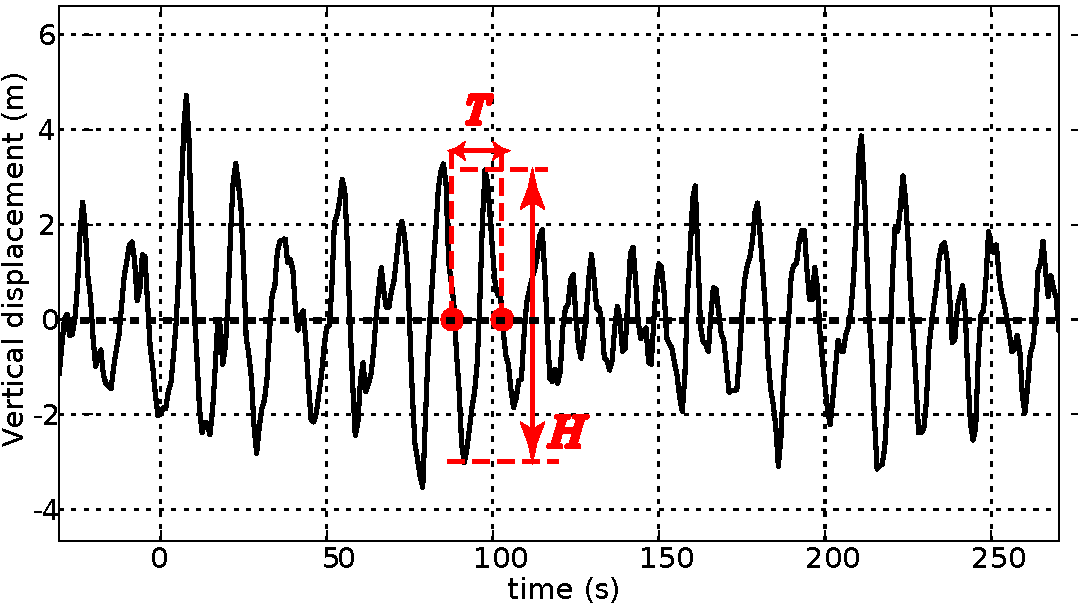
\includegraphics[width=0.8\textwidth]{FIGS_CH_INTRO/Exemple_DWIROISE2004_en.pdf}}
%\vspace{3.64in}
  \caption{Principle of wave by wave analysis: a series of elevation records is broken in individual waves of duration $T$. The separation from one 
wave to the next is the zero down-crossing of the vertical displacement. This example was obtained from a Datawell Waverider buoy deployed offshore 
of Crozon, France, in May 2004.}\label{fig:zero_crossing}
\end{figure}
%%%%%%%%%%%%%%%%%%%%%%%%%%%%%%%%%%%%%%%%%%%%%%%%%%%%%%%%%%%%%%%%%%%%%%%%%%%%%


\section{Wave-by-wave analysis\label{anavague}}
\subsection{Time series}
Time series are the most common type of measurement these days, let us see what we can learn about waves from time series. 
We shall work with series of sea surface elevation, but we could have used any other physical quantity such as the 
velocity or pressure in the water or in the air. 

We first define a single wave in time series by the time interval between two consecutive 
crossings of the mean sea level as the surface goes down, as illustrated in Fig. \ref{fig:zero_crossing}. 
The choice of 'down' instead of 'up' is fairly arbitrary but it 
keeps the forward face of the wave, which is usually  more interesting, within a single wave, whereas the rear face is split 
between two consecutive waves. 
For each wave we define a period $T$, which is the length of the time interval, and a height $H$, which is the 
difference between the maximum elevation (the crest) and the minimum elevation (the trough) during the perid. 



From a sequence of heights, we can define a probability density function (PDF) $dP$ as the limit, when $dH$ 
goes to zero, of the probability $P$ that a wave height is between $H$ and $H+dH$, divided by $dH$. 
For a statistically stationary sea state, the surface elevation is well approximated by the sum of  a large number 
of sine waves which are independent from one another. Applying the central limit theorem to this 
approximate model, we find that the surface elevation is a Gaussian process, with negative and positive anomalies around the mean sea level 
with statistics defined uniquely by the standard deviation of the sea surface elevation. As a result, and this was proven in the narrow frequency band limit 
by \cite{Rice1944} and \cite{Cartwright&Longuet-Higgins1956}, the heights follow a Rayleigh distribution, as shown on figure \ref{fig:Rayleigh}, 
 \begin{equation}
dP(H)=\frac{2H}{H_{\mathrm{rms}}^2}
\exp^{-{H^2}/{H_{\mathrm{rms}}^2}}.
\end{equation}
This PDF is normalized to give 
$\int_0^\infty dP dH =1$. The Rayleigh distribution is generally a good approximation for 98\% of the distribution, sometimes even more. 
For extreme values, a better approximation was given by \cite{Tayfun1980}, taking into account the correlations among wave components due to 
second-order nonlinearities. 
%%%%%%%%%%%%%%%%%%%%%%%%%%%%%%%%%%%%%%%%%%%%%%%%%%%%%%%%%%%%%%%%%%%%%%%%%%%%%
\begin{figure}
\centerline{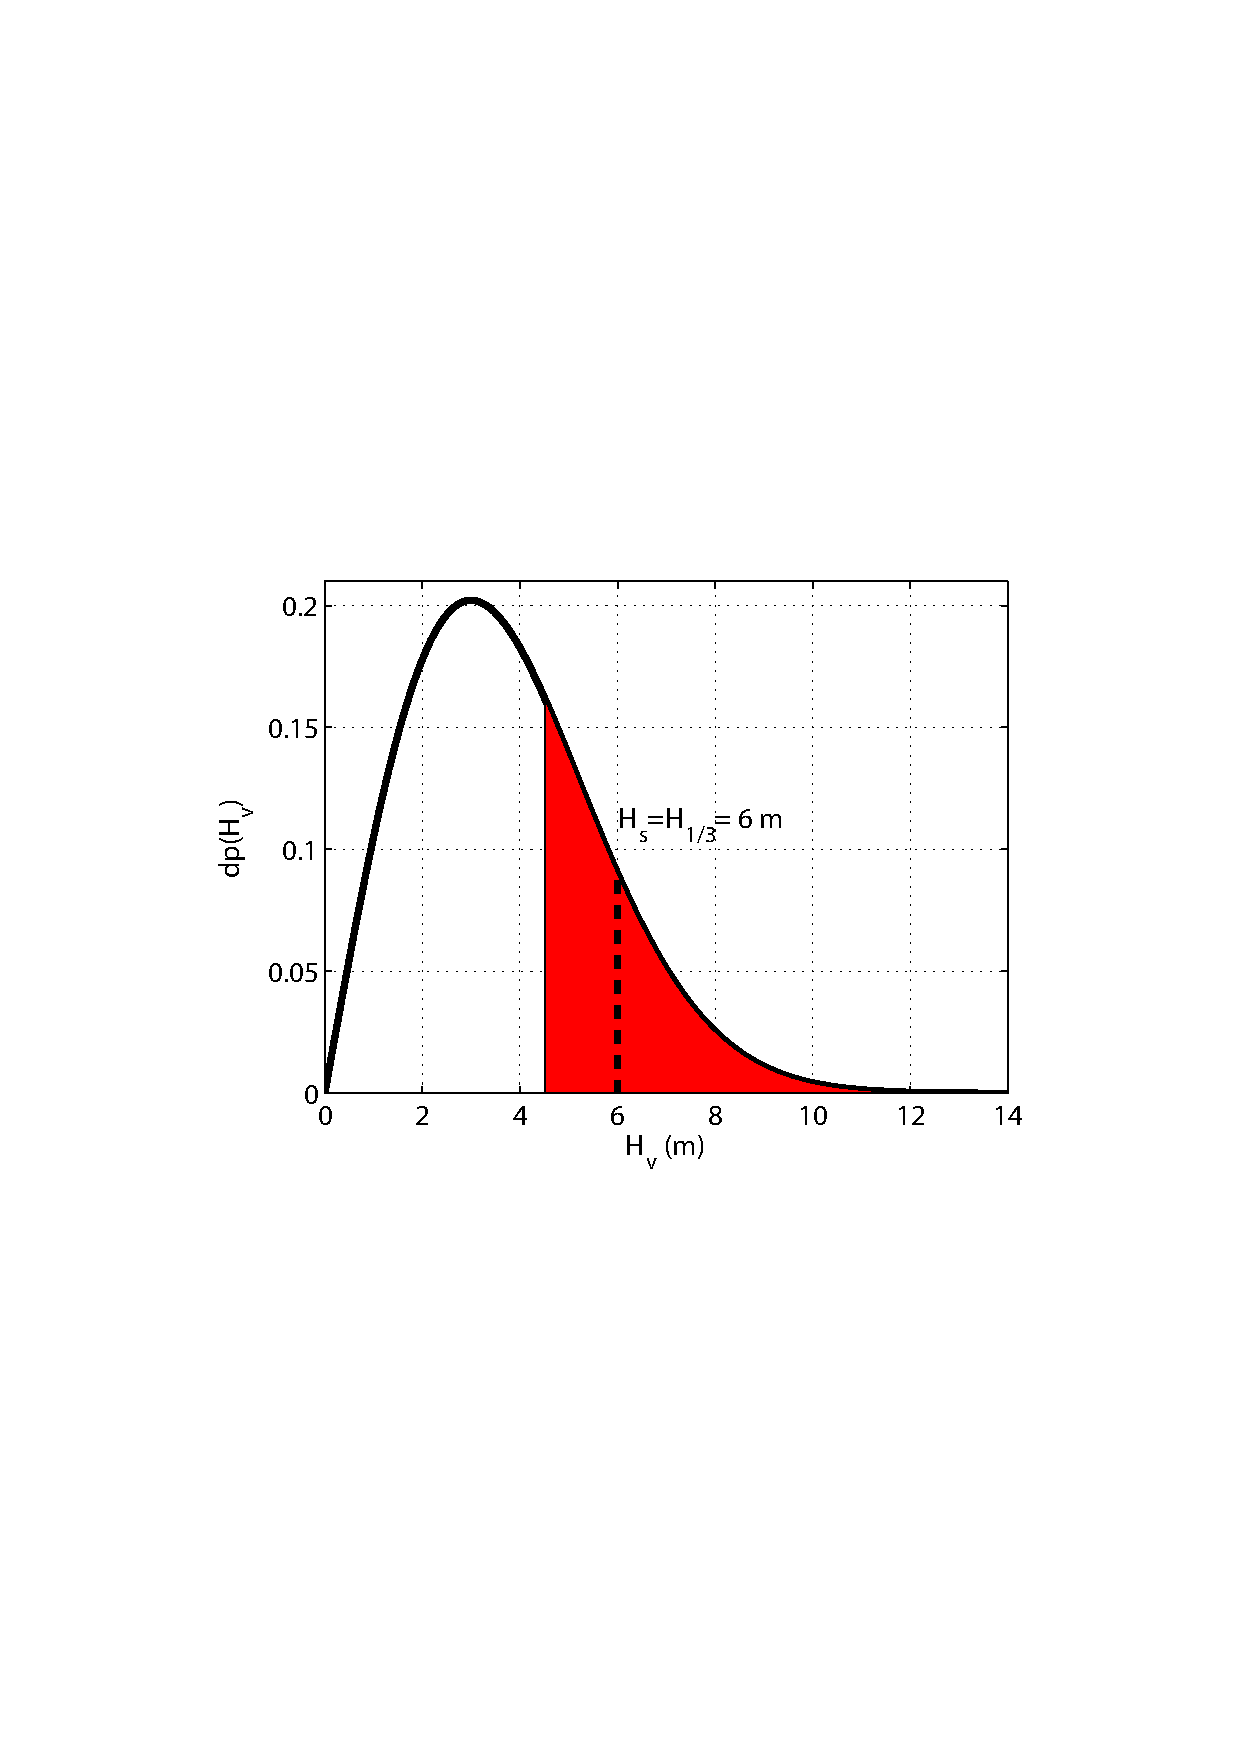
\includegraphics[width=0.6\textwidth]{FIGS_CH_INTRO/Rayleigh.pdf}}
%\vspace{3.64in}
  \caption{ Rayleigh distribution of wave heights}{$dp\times dH(H_v)$ is a probability for a single wave to have a height between  $H_v$ and $H_v+dH$. 
In red: the 1/3 of the highest waves in the distribution. The average height in this red part is $H_{1/3}$, which is one way to define the  significant wave height $H_s$. 
In the following chapters we will rather define $H_s$ as $H_{m0}$, equal to four times the standard deviation of the sea surface elevation. That other definition is 
recommended by the World Meteorological Organization and it gives a number 
very close to $H_{1/3}$.\label{fig:Rayleigh}}
\end{figure}
%%%%%%%%%%%%%%%%%%%%%%%%%%%%%%%%%%%%%%%%%%%%%%%%%%%%%%%%%%%%%%%%%%%%%%%%%%%%%

One useful result is that the probability that the height exceeds a given threshold $\widehat{H}$ 
is given by 
 \begin{equation}
P(H
>\widehat{H})=\er^{-\left(\widehat{H}/H_{\mathrm{rms}}\right)^2}\label{Hseuil}.
\end{equation}
This expression can be used to compute the height threshold $\widehat{H}$
associated to a fixed fraction of the wave population. For example 
$\widehat{H}_{1/3}$ is the height beyond which there are the highest 1/3 of the waves, and it is 
 $\widehat{H}_{1/3}=\left(\ln(3)\right)^{1/2}
H_{\mathrm{rms}}$ which is nearly 1.05$\times H_{\mathrm{rms}}$. 

A more commonly used scale for the wave heights is given by integrating 
 (\ref{Hseuil}) to get the average height of the 1/3 highest waves. This is one definition of 
the significant wave height, denoted $H_{1/3}$ or $H_s$. This scale roughly corresponds to the visual impression of wave heights, which was the most common source 
of measurements until the 1940s. 
More generally but still for a Rayleigh distribution, the average height of the $1/x$ fraction of the highest waves is, 
\begin{equation}
\left[\left(-\ln(1/x)\right)^{1/2} + \sqrt{\pi} \times
{\mathrm{erfc}}\left[\left(\ln(x)\right)^{1/2}\right]/2\right]
H_{\mathrm{rms}}
\end{equation}
 where erfc is the complementary error function.  For 
$x=1/3$, this gives $H_{1/3}=1.4157 \times H_{\mathrm{rms}}$.

From the definition, the full Rayleigh PDF $p(H)$ is determined by $H_{\mathrm{rms}}$. In practice the average $H_{1/3}$ is more 
commonly used, and there is also a lot of interest in the maximum height $H_{\mathrm{max}}$, but that one depends on the length of the 
record. When recording more waves,  $H_{\mathrm{max}}$ is likely to be higher. Waves that have a height
$H$ larger than $2.1 H_{1/3}$ are called freak waves or rogue waves. If we follow the Rayleigh statistics, 
this correspond to 1 in 5700 waves. In practice, they are a bit more frequent for conditions with large average steepnesses, as 
predicted by \cite{Tayfun1980}. Also, for real waves the spectrum is not always narrow and on average $H_{1/3} \simeq 3.8 \sqrt{m_0}$
instead of $H_{1/3} \approx 4.004 \sqrt{m_0}$, where $m_0$ is the variance of the surface elevation \citep{Goda1985}.

In the context of the design of coastal or oceanic structures,  there is a great interest in defining the 
maximum wave conditions that will occur over the expected lifetime of a structure, typically 50 to 100 years, 
or with a very low probability of occurrence to ensure maximum safety. For example, some sections of the Dutch dyke system
are required by law to resist waves that occur only once in 10,000 years. 
The material and size of the structure is then designed to withstand 
these extreme conditions. If the extreme wave height and period is overestimated, the cost of construction 
is higher than it could have been. If the conditions are underestimated, the structure is likely to fail in a time shorter
than the expected lifetime. This early failure happened for the first oil platforms built in the North Sea, in an age
when there were no routine wave measurements. 

For these extremes, the Rayleigh distribution does not hold, because the $H_s$ is itself a random variable on the 
scale of days to centuries. The extreme wave statistics on these long time scales are determined by the 
distribution of extreme meteorological event, or, in shallow water, the joint distribution of water levels (including 
the astronomical tide) with weather events. These long term statistics are clearly different from the short term statistics. 
For short term, the sea state was a superposition of many independent wave trains, and we could use the central limit theorem. 
For long terms, we first need to determine the distribution of the significant wave heights  $H_{s}$, and the probability 
that the height of a single wave exceeds $H_0$ is then the conditional 
probability $p(H > H_0  | H_s = H_{s0})$. The distribution of $H_s$ follows a generalized Pareto distribution, 
and the probability $p(H > H_0)$ is given by integrating the conditional probability over $H_{s0}$. 

Obviously, this requires stationary statistics. In some regions 
these statistics fluctuate with climatic patterns like the North Atlantic Oscillation, which particularly impacts
the wave heights on the European Atlantic coast, or the El Nino-Southern Oscillation  (ENSO) which has a strong 
impact on waves in the central Eastern Pacific or on the U.S. West coast \citep{Bromirski&al.2005}. 
As an example, Edward Thornton, a renown specialist of nearshore dynamics, was asked in 1996 to provide 
some consulting advice for the construction of a wastewater pipeline in Monterey Bay, Central California. 
Construction started in 1997 in the middle of a very strong El Nino, 
the hundred-year wave height, which had been properly evaluated by Ed Thornton, was exceeded 
and the half-ton rocks protecting the pipe were too small to stay in place and were dispersed by the waves. 
For such a strong El Nino event, the storm waves that caused the damage on the U.S. West Coast were normal. 
One should thus use statistics with caution. Defining extreme wave heights is also very challenging in tropical areas where
they are associated with hurricanes that have random tracks: a 20-year record of hurricane tracks generally does not contain 
all possible tracks, in particular the one of the next hurricane that will destroy this or that facility. 
Finally, there are also long-term trends associated with global change \citep[e.g.][]{Wang&Swail2002,Charles&al.2012}, 
especially in the Arctic where the trend in sea ice extent  is leading to higher wave heights and periods \citep{Stopa&al.2016b}. 

\subsection{Maps}
Wave statistics from time series cannot represent all wave properties. Some of these, such as the 
length of crests, are defined from the spatial 
patterns in the wave field. This parameter, although secondary to the wave height, gives information 
on the spatial coherence of wave-induced motions and is thus very important when navigating a seaway or designing 
a structure that may be wider than the crest length.
 
Just like we have defined heights and periods, heights and lengths $L$ can be defined 
in the case of waves propagating all in the same direction, say $x$. In that case, the crests are infinitely long in the other 
direction $y$. One important parameter is then the wave slope, defined from the ratio $H/L$. For sinusoidal waves, the maximum 
slope is $\pi H/ L$. 

Things get more complex when considering real waves that propagate in all directions. 
One can use the theory of random fields, developed by \cite{Adler1981}. In that theory, the crests are defined 
as subsets of the horizontal plane that are simply connected and that are above the mean sea level. Using this definition 
requires a bit of topology. In this context it becomes more difficult to associate a crest with a trough. 
There is a strong development of spatial statistics for ocean engineering and oceanography, thanks to the development 
of video measurement techniques \citep{Fedele&al.2009a}. 

\cleardoublepage
\chapter{Main properties of linear waves}\label{ch1b}
This chapter explains how and why water moves in waves, once the waves have been generated. 
A more logical sequence might have been to study the generation process of the waves first, but it is much more complex 
and can only be understood once one knows how the waves move. The properties exposed in this chapter
are independent of the generation mechanism, and thus common to all surface gravity waves, including tsunamis, ship wakes, and wind-generated waves. 

In order to make things simple, we consider a flat, non-deformable bottom 
located at $z=-h$, and periodic waves in both space and time. This may sound very restrictive, but waves at 
sea generally behave as if the bottom were locally flat, and the periodicity allows us to study elementary waves 
that are later superimposed thanks to the quasi-linear wave motion, with some possible non-linear corrections to better fit
the equations of motion. We will thus start with the linear wave theory of unidirectional and monochromatic 
waves that was first developed by  \cite{Airy1841}, and which is a good approximation for waves of small height in not-too-shallow water. 
These are the typical conditions found in swells for depths larger than 50~m or so. Swells are the waves generated by winds in remote storms. 
It is also instructive for the oceanographer to play the game of differences, and find the common traits and main differences 
between these swells, and the tidal waves in shallow water that take the form of  Kelvin waves. In fact, most 
of the wave properties derived here also apply to Kelvin waves. The main difference is the geostrophic balance along the crest of Kelvin waves 
that does not exist for shorter gravity waves for which the Coriolis force can be neglected for most properties. 


We will try here not to get carried away by mathematics, which are necessary to arrive at quantitative predictions.
Instead we will use the equations only as tools to help us reveal the wave motion in terms of forces, pressure and flow, which should 
help us navigate the many simplifying assumptions ot understand the role term. 

\section{Waves: a question of gravity, pressure, mass and vorticity}
Before jumping into equations, we should make a few mechanical remarks. 
There is a motion in and above waves because the crests and troughs of the sea surface, located at $z=\zeta(x,y,t)$, 
correspond to different weights of water, which 
creates a pressure difference. We can already note that these pressure variations 
are of the order of $\rho_w g \zeta$, with $\rho_w$ the water density and $g$ the vertical apparent\footnote{Apparent means that 
this is not just Newton's general gravitation but it also includes the centrifuge acceleration due to the Earth rotation, giving 
$g \simeq 9.81$m s$^{-2}$.} acceleration of gravity. With a 1~m difference in height from crest to trough, 
we get a pressure difference of 10 kPa. What is important for the motion is the pressure \emph{gradient}. With a wavelength 
of 200~m, this gives a crest-to-trough pressure gradient of the order of 100 Pa/m at the same level $z$, 
which drives a horizontal acceleration of 0.1~m/s$^2$. 

The water set in motion flows in an orderly way, following several principles. 
First, the mass of water is conserved, and for the slow velocities considered in this chapter, the flow is 
incompressible, hence non-divergent. We will also consider that the bottom does not deform under the waves. 
As a result, the horizontal convergence between a crest and the next trough must give 
rise to a vertical divergence. Besides, because the waves are generated by pressure forces, and propagated by pressure forces, 
the motion is, in a first approximation, irrotational. The vertical and horizontal velocities are thus strongly constrained by 
these two properties: \textbf{incompressibility} and \textbf{zero vorticity}.

In summary, the free surface position $\zeta$ and gravity determine the near-surface pressure $p$, which gives the horizontal velocity $u$. 
The vertical velocity $w$ is determined from the horizontal velocity using the 
zero divergence and vorticity conditions, and $w$ also modifies the pressure field. We thus can express 
the problem of wave mechanics as a set of four equations for the four unknowns that are $\zeta$, $p$, $u$ and $w$. 
%%%%%%%%%%%%%%%%%%%%%%%%%%%%%%%%%%%%%%%%%%%%%%%%%%%%%%%%%%%%%%%%%%%%%%%%%%%%%
\begin{figure}
\centerline{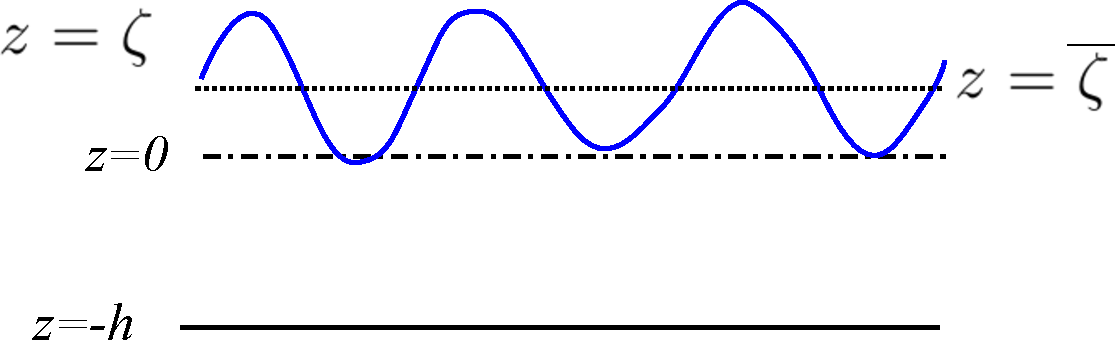
\includegraphics[width=0.5\textwidth]{FIGS_CH_AIRY/vertical_coord_def.pdf}}
%\vspace{3.64in}
  \caption{Definition of vertical levels: $\zeta$ is the sea level, $-h$ is the bottom, both defined relative to an arbitrary vertical datum $z=0$. As a result the
mean water depth is $D=h+\overline{\zeta}$.}
\label{fig:Dandh}
\end{figure}
%%%%%%%%%%%%%%%%%%%%%%%%%%%%%%%%%%%%%%%%%%%%%%%%%%%%%%%%%%%%%%%%%%%%%%%%%%%%%

\section{Wave mathematics}
We shall see that two important quantities, the wavelength $L$ and period $T$ are closely related 
for waves of small amplitude $a$. Here we define "small" to  mean that both the sea surface slope $ka$ and non-dimensional depth $a/D$ are small, 
where $k=2\upi/L$ is the wavenumber, and $D=h+\zb$, is the mean water depth. We remind the reader that $z=-h$
is the vertical position of the bottom, and $\zb$ is the mean sea surface elevation, both relative to an arbitrary datum 
$z=0$.

These small parameters $ka$ and $a/D$ will appear repeatedly in this book. Their ratio gives a third parameter, which is independent 
of the wave amplitude, and that will be very important for the wave kinematics, this is the 
\textbf{non-dimensional depth} $kD$.

We will now go into the details of the linear wave theory, first 
laid out by Airy in the 19th century. It has the great advantages of being  \textbf{linear}, hence any combination of the 
linear solution is also a solution of the equations of motion. More importantly, this linear model explains many of the waves properties, 
and is very accurate for swells in not-too-shallow water, and is not too far off for most wave properties, even for waves 
breaking in the surf zone.  

Let us make two final remarks before we get into the equations. 
First, the linear waves exist only on paper, as all monochromatic waves are unstable, with a development of this instability 
that is faster for higher waves. This aspect is discussed in more details in chapters \ref{ch_sourceterms} and Part 3. 
Monochromatic waves are an acceptable solution for short evolution times, at least a few periods, possibly much more. Second, 
the choice of the Eulerian framework for the equations of motion
is not a very good choice for the accuracy, as the linear Lagrangian theory 
is much more accurate than the Eulerian theory of Airy, because of the very simple balance between the pressure gradient and the 
fluid parcel acceleration.  
\cite{vonGerstner1809} did find an exact theory that exactly satisfies the condition $p=p_a$ at the free surface, 
but it has an non-zero vorticity, which must be compensated by a sheared current. 
The use of Lagrangian equations is unfortunately 
more complex, and this is the main reason why we do not use it here. It is interesting to note, that 
mass conservation is linear in an Eulerian framework, 
while momentum conservation is non-linear, but the opposite is true for a Lagrangian framework. 

\section{Eulerian equations for wave motion}
Our starting point is the conservation of mass and momentum applied to 
the ocean, with the former reduced to a zero divergence as we consider a constant density, which is 
true for the ocean within a few parts per thousand, and incompressible flow. 
The horizontal position is defined by the two-component vector 
${\mathbf x}=\left(x,y\right)$ and the vertical is $z$. The corresponding velocities are 
${\mathbf u}=\left(u,v\right)$ and $w$. Considering sea water as a perfect fluid, 
we apply the Navier-Stokes equations, 
\begin{equation}
    \frac{\partial {\mathbf u}}{\partial t}+{\mathbf u}\bcdot\bnabla{\mathbf u}
    + w \frac{\partial {\mathbf u}}{\partial z}
    =-\frac{1}{\rho_w} \bnabla p +
    \nu \left(\nabla^2 {\mathbf u}+\frac{\partial^2 u}{\partial z^2}\right),
    \label{NSxy}
\end{equation}
\begin{equation}
    \frac{\partial w}{\partial t}+{\mathbf u}\bcdot\bnabla w
    + w \frac{\partial w}{\partial z}
    =-g - \frac{1}{\rho_w} \frac{\partial p}{\partial z} +
    \nu \left(\nabla^2 w+\frac{\partial^2 w}{\partial z^2}\right),
    \label{NSz}
\end{equation}
\begin{equation}
\bnabla\bcdot{\mathbf u} + \frac{\partial w}{\partial z}=0,
\end{equation}
where $\bnabla$ is the horizontal gradient operator. We thus have \textbf{four scalar equations} since \ref{NSxy} has two horizontal components
for the \textbf{four unknowns} that are $u$, $v$,
 $w$ and $p$. Our problem will be well posed as soon as we define the boundary conditions, from the continuity of 
velocity and or stresses (pressure and shear stresses) and initial conditions. At the bottom, we only impose a free slip
 \begin{equation}
w=-{\mathbf u} \bcdot \bnabla h \quad \mbox{at} \quad
z=-h\left({\mathbf x}\right)
\end{equation}
which simplifies to $w=0$ because we chose $h$ to be constant

At the surface, we make the further hypothesis that for any horizontal position $\mathbf{x}$ there is only one value $z=\zeta$ 
of the free surface position (this excludes an overturning of the surface, as found in plunging breakers). 
The free surface is a material surface, which means that water parcels on the surface must stay on the surface. 
This can be expressed by the condition 
\begin{equation}
    \frac{\rm d}{dt}\left(z-\zeta\right)=
    w - {\mathbf u} \bcdot \bnabla \zeta -\frac{\partial \zeta }{\partial t}= 0
    \quad \mbox{at\ }\quad z=\zeta.\label{eq:skbc}
\end{equation}
An interpretation of this surface kinematic boundary condition 
is that the vertical motion 
${\partial \zeta }/{\partial t}$ is the combination of the vertical velocity 
$w$ and the horizontal advection of the water parcels sliding along the surface ${\mathbf u} \bcdot \bnabla \zeta$.

To that kinematic boundary condition we add the dynamic boundary condition that express the continuity of 
stresses at the air-sea interface. Neglecting the wind stress and surface tension, these reduce to a continuity of 
the pressure. In this chapter we will assume that the atmospheric pressure is takes the constant value  $p_a$,
\begin{equation}
    p=p_a\quad \mbox{at\ }\quad z=\zeta.
\end{equation}

We now assume irrotational motion, so that the velocity field 
is given by the gradient of a velocity potential 
$\phi$. Namely, $ {\mathbf u} = \bnabla \phi$ and $w={\partial
\phi}/{\partial z}$. In this and all our notations, the classical operators  (gradient
$\bnabla$, Laplacian $\Delta$ ...) are restricted to the horizontal 
plane, in order to simplify notations. This assumption of irrotational wave motion
is generally consistent with observations of real waves. Still, the vorticity can be 
very strong locally, for example in in the bottom and surface boundary layers
or just after a wave has broken. Also, in the presence of sheared currents, the wave motion always has 
some vorticity, and a weak vorticity also arises from the Earth rotation. 
%Il faut noter que cette condition n'est
%n\E9cessaire qu'\E0 un instant donn\E9: un mouvement initialement
%irrotationnel reste irrotationnel. 
We finally start off by neglecting the viscous terms in the Navier-Stokes equations. This is justified by the 
fact that any significant 
wave-induced motion has scales of velocity $U$ and length $L$ that are large enough to 
make the Reynolds number $UL/\nu$ of the order of  10$^4$ or more.

All the assumptions made above remove some real features in the wave motion. 
Real waves always have some vorticity, which is also linked to the viscosity 
effects in the boundary layers. A rigorous treatment of these effects is possible 
and will be discussed in other chapters. We are here looking for the most 
simple solution that will capture most of the important properties of real waves. 


Replacing velocities by gradients of $\phi$ in
(\ref{NSxy})--(\ref{NSz}) one arrives at
\begin{equation}
    \bnabla \left[\frac{\partial \phi}{\partial t}
    +\frac{1}{2}\left(
    \left|\bnabla \phi\right|^2
    +\left(\frac{\partial \phi}{\partial z}\right)^2
    \right)
    +\frac{p}{\rho_w}+gz \right]=0,
\end{equation}
and
\begin{equation}
    \frac{\partial}{\partial z} \left[\frac{\partial \phi}{\partial t}
    +\frac{1}{2}\left(
    \left|\bnabla \phi\right|^2
    +\left(\frac{\partial \phi}{\partial z}\right)^2
    \right)
    +\frac{p}{\rho_w}+gz \right]=0.\label{eq:NStoBer}
\end{equation}
These two equations establish that the term in brackets is not a function of position and can 
only be a function of time $\gamma(t)$, 
\begin{equation}
    \frac{\partial \phi}{\partial t}
    +\frac{1}{2}\left(
    \left|\bnabla \phi\right|^2
    +\left(\frac{\partial \phi}{\partial z}\right)^2
    \right)
    +\frac{p}{\rho_w}+gz =\gamma(t).\label{eq:Bernoulli}
\end{equation}

The other important equation given by the conservation of mass is linear, 
The mass conservation equation was already linear, 
\begin{equation}
\bnabla \bcdot {\mathbf u} + \frac{\partial w}{\partial z} =0
\end{equation}
and is equivalent to Laplace's equation for $\phi$
\begin{equation}
    \bnabla^2 \phi + \frac{\partial^2 \phi}{\partial z^2}=0,
    \quad \mbox{at\ }\quad -h\leq z \leq \zeta. \label{Laplace}
\end{equation}


\section{Small slope waves over a flat bottom: the Airy solution}
So far, we had only assumed an incompressible flow (assumption A1), zero viscosity (A2), 
irrotational motion (A3), a flat bottom (A4). 

% and a sinusoidal  et que
%le potentiel des vitesses varie spatialement comme une sinuso\EFde
%(H5). 

We shall now linearize the momentum equation (\ref{eq:Bernoulli}), assuming that the wave amplitude is small enough to 
neglect the non-linear terms. This is verified in chapter Part 3, provided that 
the wave amplitude $a$ is much less than the wavelength $L$ and $a$ is much less than the mean water depth $D$. 


This gives the linearized Bernoulli equation
\begin{equation}
    \frac{\partial \phi}{\partial t} \simeq 
       -\frac{p}{\rho_w}-g z + \gamma(t).\label{Bernoulli_lin}
\end{equation}
Assuming that waves are propagating \footnote{In the presence of standing waves, $\gamma(t)$ 
is an oscillating function of the order of $g a^2/L$, as derived by \cite{Miche1944d}.  \cite{Longuet-Higgins1950} further showed that this pressure field is actually an acoustic wave when the water compressibility is considered, which explains the generation of seismic and acoustic waves by ocean wind-generated waves.} at a speed $C$, the motion is periodic as a function of $x-C t$ and thus $\gamma(t)$ is a true constant, that can be determined from the dynamic boundary condition $p=\overline{p}_a$ at $z=\zeta$,
This gives the pressure as a function of the velocity potential, for $z< \zeta$, 
\begin{equation}
    p=\overline{p}_a -{\rho_w}g(z-\zeta) 
    -\rho_w \frac{\partial \phi}{\partial t}.\label{p_all}
\end{equation}
The Bernoulli equation states that the pressure is the hydrostatic pressure plus some correction 
due to the non-stationary motion. The static pressure term has been removed by the linearization. 

The linearized kinematic boundary condition, which expresses the continuity of velocities, reads
\begin{equation}
    w = \frac{\partial \phi }{\partial z} \simeq \frac{\partial \zeta}{\partial t}
    \quad \mbox{at\ }\quad z=\zeta,  \label{surface_lin}
\end{equation} which corresponds to a flat sea surface approximation. 
We can further approximate that the actual sea level is not too far from the mean sea level $z=\overline{\zeta}$. 


Finally, the bottom kinematic boundary condition becomes, 
\begin{equation}
    w=\frac{\partial \phi }{\partial z}=0 \quad \mbox{sur\ }\quad z=-h.  \label{bottom}
\end{equation}

Taking  $\partial (\ref{Bernoulli_lin} \textrm{~at z=}\zeta)/\partial t $
+$g\times$(\ref{surface_lin}) we eliminate the unknown $\zeta$, and obtain our 
wave equation 
\begin{equation}
  \frac{\partial^2{\phi}}{\partial{t^2}}+g\frac{\partial\phi}{\partial z}=0, \quad \mbox{at}
\quad  z=\overline{\zeta}. \label{surface 1}
\end{equation}

Equations (\ref{bottom})--(\ref{surface 1}) are the bottom and top boundary conditions for Laplace's equation. The 
set of equation  (\ref{Laplace})--(\ref{surface 1}) is
usually called the Euler equation. Its full non-linear form is given in Part 3. 
 
\subsection{Solution: Laplace equation and vertical profiles}
Since we have a linear wave equation, it is natural to solve it 
using the Fourier transform that gives us a full basis of solutions. Without loss of generality, 
we thus look for solutions of the form, 
\begin{equation}
    \phi=\Re \left(\widetilde{\phi}\left(z\right)
     \mathrm{e}^{\mathrm{i}{\mathbf k}\bcdot{\mathbf x} - \sigma t} \right),
    \label{phi1}
\end{equation}
where $\Re(x)$ is the real part of $x$. Replacing in Laplace's equation gives the Helmolz equation 
\begin{equation}
    -k^2 \widetilde{\phi}+\frac{\partial^2 \widetilde{\phi}}{\partial z^2}=0.
    \label{Helmholz}
\end{equation}
Any solution is thus the sum of two exponentials, which can be recombined in the form 
\begin{equation}
    \widetilde{\phi}(z)=A \cosh\left(kz+kh \right)
        + B \sinh\left(kz+kh \right).
\end{equation}
The bottom boundary condition imposes that $B=0$, and we thus only keep the first term,
\begin{equation}
    \widetilde{\phi}\left(z\right)=\Phi_0
    \frac{\cosh\left(kz+kh\right)}{\cosh\left(kD\right)}.
    \label{cosh}
\end{equation}

Considering that the amplitude of the vertical velocity $w=\partial \widetilde{\phi} / \partial z$ at the surface, where $z+h=D$,  is the radian frequency $\sigma$ times the elevation amplitude $a$, 
we have 
\begin{equation}
    | \Phi_0 |   k \sinh (kD) / \cosh (kD) = \sigma a.
\end{equation}
Hence, from Laplace's equation alone we get the orbital velocities. Wave motion has a maximum horizontal speed at the crest with a magnitude  $\sigma a / \tanh(kD)$, and in the direction 
of propagation. Because of the Laplace equation, when $kD >> 1$ the motion decays exponentially away from the surface over a typical distance that is $1/k=L/2\pi$.

%The only fact that the velocity potential is a solution to Laplace equation gives important analogies with many other waves but also other physical phenomena: electromagnetic waves are also surface waves with "skin effects" when considering high enough frequencies. 


\subsection{Solution: Momementum balance and dispersion relation}
Replacing $\phi$ by eq. (\ref{phi1}) using (\ref{cosh}) in the wave equation (\ref{surface 1}) gives  
\begin{equation}
    - \sigma^2 \Phi_0 +gk\tanh\left(kD\right)\Phi_0=0.
     \label{onde 1}
\end{equation}
This equation expresses the balance of forces between the horizontal pressure gradient which, just below the surface is 
is hydrostatic, with an amplitude  $\rho_w g a k$, and the horizontal acceleration, which has an amplitude  $\sigma^2 a / \tanh(kD)$. 
This is the dispersion relation for linear waves over a flat bottom, first given by \cite{Laplace1776}, 
\begin{equation}
    \sigma^2=g k \tanh\left(kD\right).
     \label{dispersion}
\end{equation}
As a result, where $D$ is reduced but $\sigma$ is constant, waves have a lower phase speed $C=\sigma/k$  for example near the shoreline. 
Contrary to a widespread misconception, this reduction of the phase speed has nothing to do with bottom friction.
in fact the wave orbital velocity increases, and in the Airy theory there is no dissipation of energy.




\subsection{Solution: polarization relations}
Having solved for the velocity potential, we can now link it back to the surface elevation using eq. (\ref{surface_lin}). 
Defining the phase of the free surface elevation, 
\begin{equation}
   \Theta={\mathbf
k}\bcdot{\mathbf x}-\sigma t+ \Theta_0, \label{eq:phase}
\end{equation}
 with $\Theta_0$ a constant between 0
et $2\pi$, eq. (\ref{surface_lin}) links the surface elevation amplitude $a$ and the amplitude $\Phi_{0}$ of the velocity potential at the surface 
\begin{equation}
    a={\mathrm i}\frac{\sigma}{g}\Phi_{0},\label{afromPhi0}
\end{equation}
the elevation, velocities and pressure of the \cite{Airy1841}\footnote{Although 
Laplace, Cauchy and Poisson gave all elements of this theory many years 
before Airy, the latter was the first to address the problem of a single propagating monochromatic 
wave train. Poisson solved several problems of greater complexity, including stationary waves 
and circular waves \citep{Craik2004}.} We thus have  the  following 
polarization relations that link the amplitudes and phase of all oscillating variables 
\begin{equation}
    \zeta-\overline{\zeta}=a \cos \Theta,\label{polzeta}
\end{equation}
and the velocity potential 
\begin{equation}
    \phi=  \frac{a}{k}\sigma
    \frac{\cosh\left(kz+kh\right)}{\sinh\left(kD\right)}
    \sin \Theta.
      \label{potentielcos}
\end{equation}
gives the velocity field
\begin{equation}
    \ub= a \frac{{\mathbf k}}{k}\sigma
    \frac{\cosh\left(kz+kh\right)}{\sinh\left(kD\right)}
    \cos \Theta,
      \label{vitesse}
\end{equation}
\begin{equation}
    w=a \sigma
    \frac{\sinh\left(kz+kh\right)}{\sinh\left(kD\right)}
    \sin \Theta. \label{eq:w}
\end{equation}
The pressure field is obtained from the linearized Bernoulli equation with the constant 
given by the dynamic surface boundary condition, as in eq. (\ref{p_all}), 
\begin{equation}
    p=\overline{p}^H+\rho_w g a
    \frac{\cosh\left(kz+kh\right)}{\cosh\left(kD\right)}
    \cos \Theta,
      \label{pression}
\end{equation}
where the hydrostatic pressure is $\overline{p}^H=-\rho_w g
(z-\zb)+\overline{p}_a$ with ${p}_a$ the atmospheric pressure. 
We also have




%et la fonction de courant
%\begin{equation}
%    \psi=  \frac{a}{k}\sigma
%    \frac{\sinh\left(kz+kH\right)}{\sinh\left(kD\right)}
%    \cos \left({\mathbf k}\bcdot{\mathbf x}-\sigma t + \Theta \right),
%      \label{vitesse}
%\end{equation}


We obtain the displacements of water particles by integrating the velocity field in 
time. To a first order of approximation (at first order in $\varepsilon=ka$),
we have the horizontal displacement
\begin{equation}
     \widetilde{\xi}_h = - a \frac{{\mathbf k}}{k}
    \frac{\cosh\left(kz+kh\right)}{\sinh\left(kD\right)}
    \sin \Theta,
      \label{xi1}
\end{equation} and the vertical displacement
\begin{equation}
    \widetilde{\xi}_3 =a
    \frac{\sinh\left(kz+kh\right)}{\sinh\left(kD\right)}
    \cos \Theta \label{xi3}.
\end{equation}
Because of the wave propagation, the water parcels spend more time under the crest, where the horizontal 
velocity is larger, than under the trough, where the velocity is weaker. As a result there is a net, order $(ka)^2$ drift in the direction 
of propagation, even for linear waves. This is a Stokes drift - it is also called the wave (pseudo)-momentum. Like the energy and the wave action, the Stokes 
drift is an intrinsic quadratic property 
of the wave field. This aspect is discussed in more details in chapter \ref{ch_momentum}. 

Eq. (\ref{dispersion})--(\ref{potentielcos}) are all approximate solutions corresponding to the Airy waves. \cite{Stokes1849} extended this Airy solution 
to take into account the non-linear terms of the full equation (see Part 3), which improves the agreement with observations.
In the deep ocean, all measurements confirm that waves are very nearly irrotational and well described
by the theories of Airy and Stokes
\citep[see for example ][]{Thornton&Kraphol1974,Herbers&al.1992}. The general solution can be expressed as a 
series in powers of 
$\varepsilon_1=ka$, which was shown to converge by \cite{Levi-Civita1925}. Many methods have been developed to 
obtain various numerical approximations of the exact solution.

\subsection{Physical interpretation}
The wave motion is maintained by the restoring force of gravity, which acts in quadrature to the velocity field, 
and thus always overshoots the equilibrium and creates crests where there were troughs. 
The acceleration induced by the pressure field feeds back into the pressure, and the motion \emph{is not} hydrostatic. 
Near the surface, the pressure is nearly hydrostatic (figure \ref{fig:puv1}). If the depth is large enough, 
at some level the vertical acceleration eventually cancels the pressure oscillations so that there is no 
significant motion at a depth much larger than the wavelength. This is typical of a surface wave, the motion decays exponentially 
from the surface, it is 'evanescent' or 'inhomogeneous'. 
%%%%%%%%%%%%%%%%%%%%%%%%%%%%%%%%%%%%%%%%%%%%%%%%%%%%%%%%%%%%%%%%%%%%%%%%%%%%%
\begin{figure}
\centerline{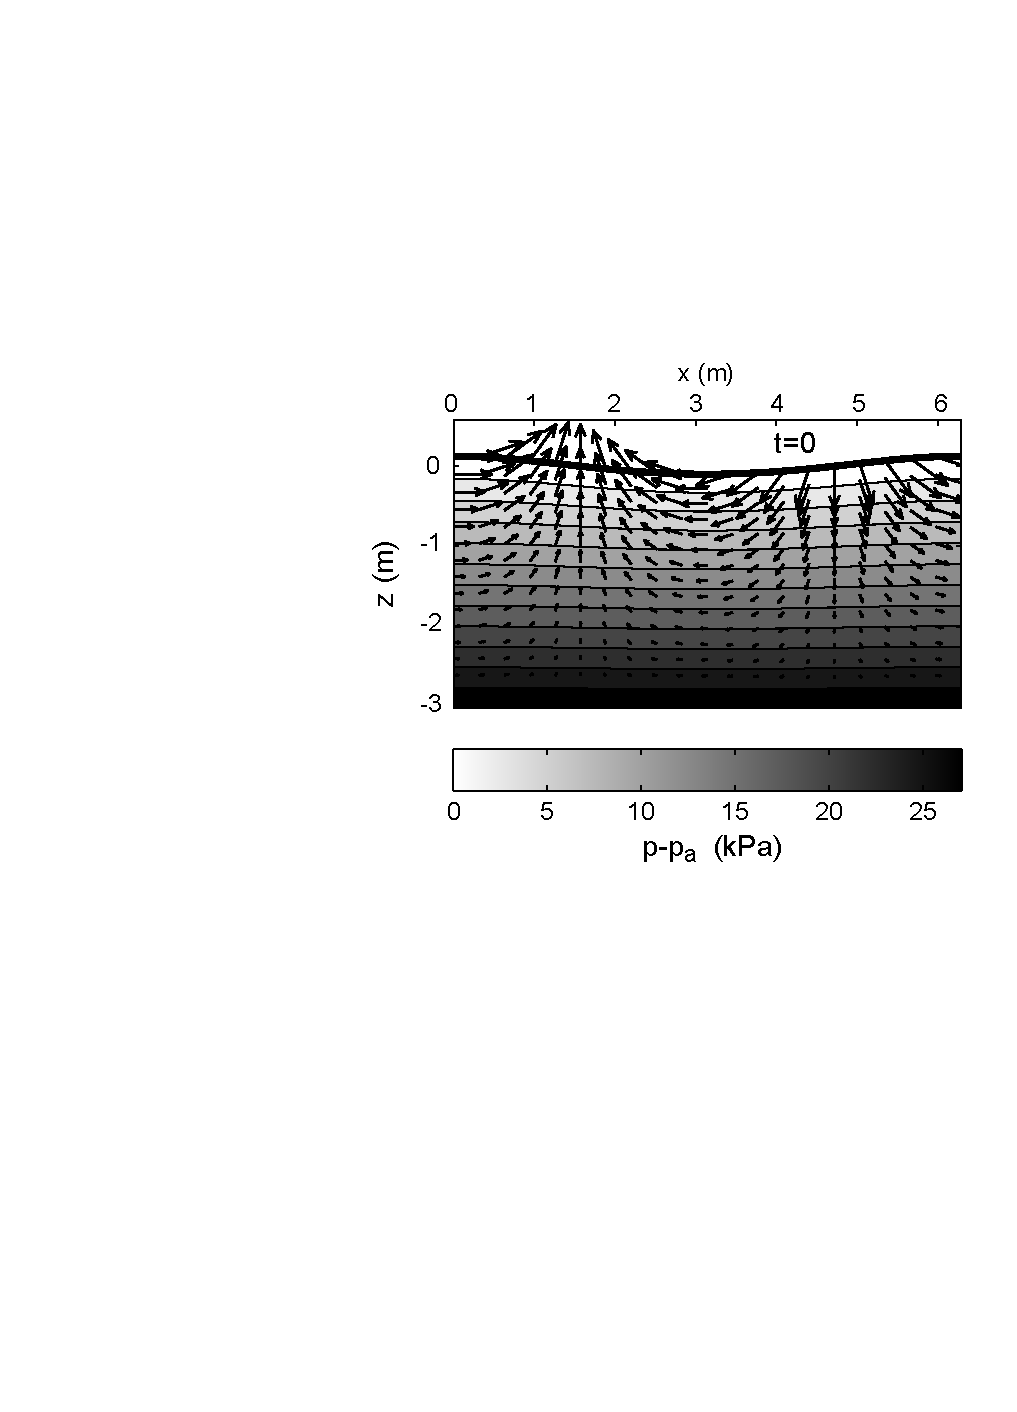
\includegraphics[width=0.6\textwidth]{FIGS_CH_AIRY/2sec_3mdepth_ppuv_1.pdf}}
%\vspace{3.64in}
  \caption{Pressure and velocity fields for a monochromatic wave of 
period $T=2$~s in a mean water depth of  $D=3$~m.}
\label{fig:puv1}
\end{figure}
%%%%%%%%%%%%%%%%%%%%%%%%%%%%%%%%%%%%%%%%%%%%%%%%%%%%%%%%%%%%%%%%%%%%%%%%%%%%%

The flow is better understood by looking at the pressure $p$ 
corrected for a hydrostatic pressure $p^H=p_a-\rho_w g (z-\overline{\zeta})$. This reveals a striking property, 
which is only true for $kD \gg 1$, the isobars of $p-p^H$ are also the streamlines. The streamfunction 
$\psi$ is such that $u=\partial \psi/\partial z$, which gives
\begin{equation}
    \psi=  \frac{a}{k}\sigma
    \frac{\sinh\left(kz+kD\right)}{\sinh\left(kD\right)}
    \cos \Theta,
      \label{potentiel}
\end{equation}
which is, for $kD\rightarrow \infty$ the pressure times $\rho_w g k$. 
This flow is in cyclostrophic equilibrium: the pressure gradient balances the 
centrifugal force of a water parcel turning around its circular orbit. 
%%%%%%%%%%%%%%%%%%%%%%%%%%%%%%%%%%%%%%%%%%%%%%%%%%%%%%%%%%%%%%%%%%%%%%%%%%%%%
\begin{figure}
\centerline{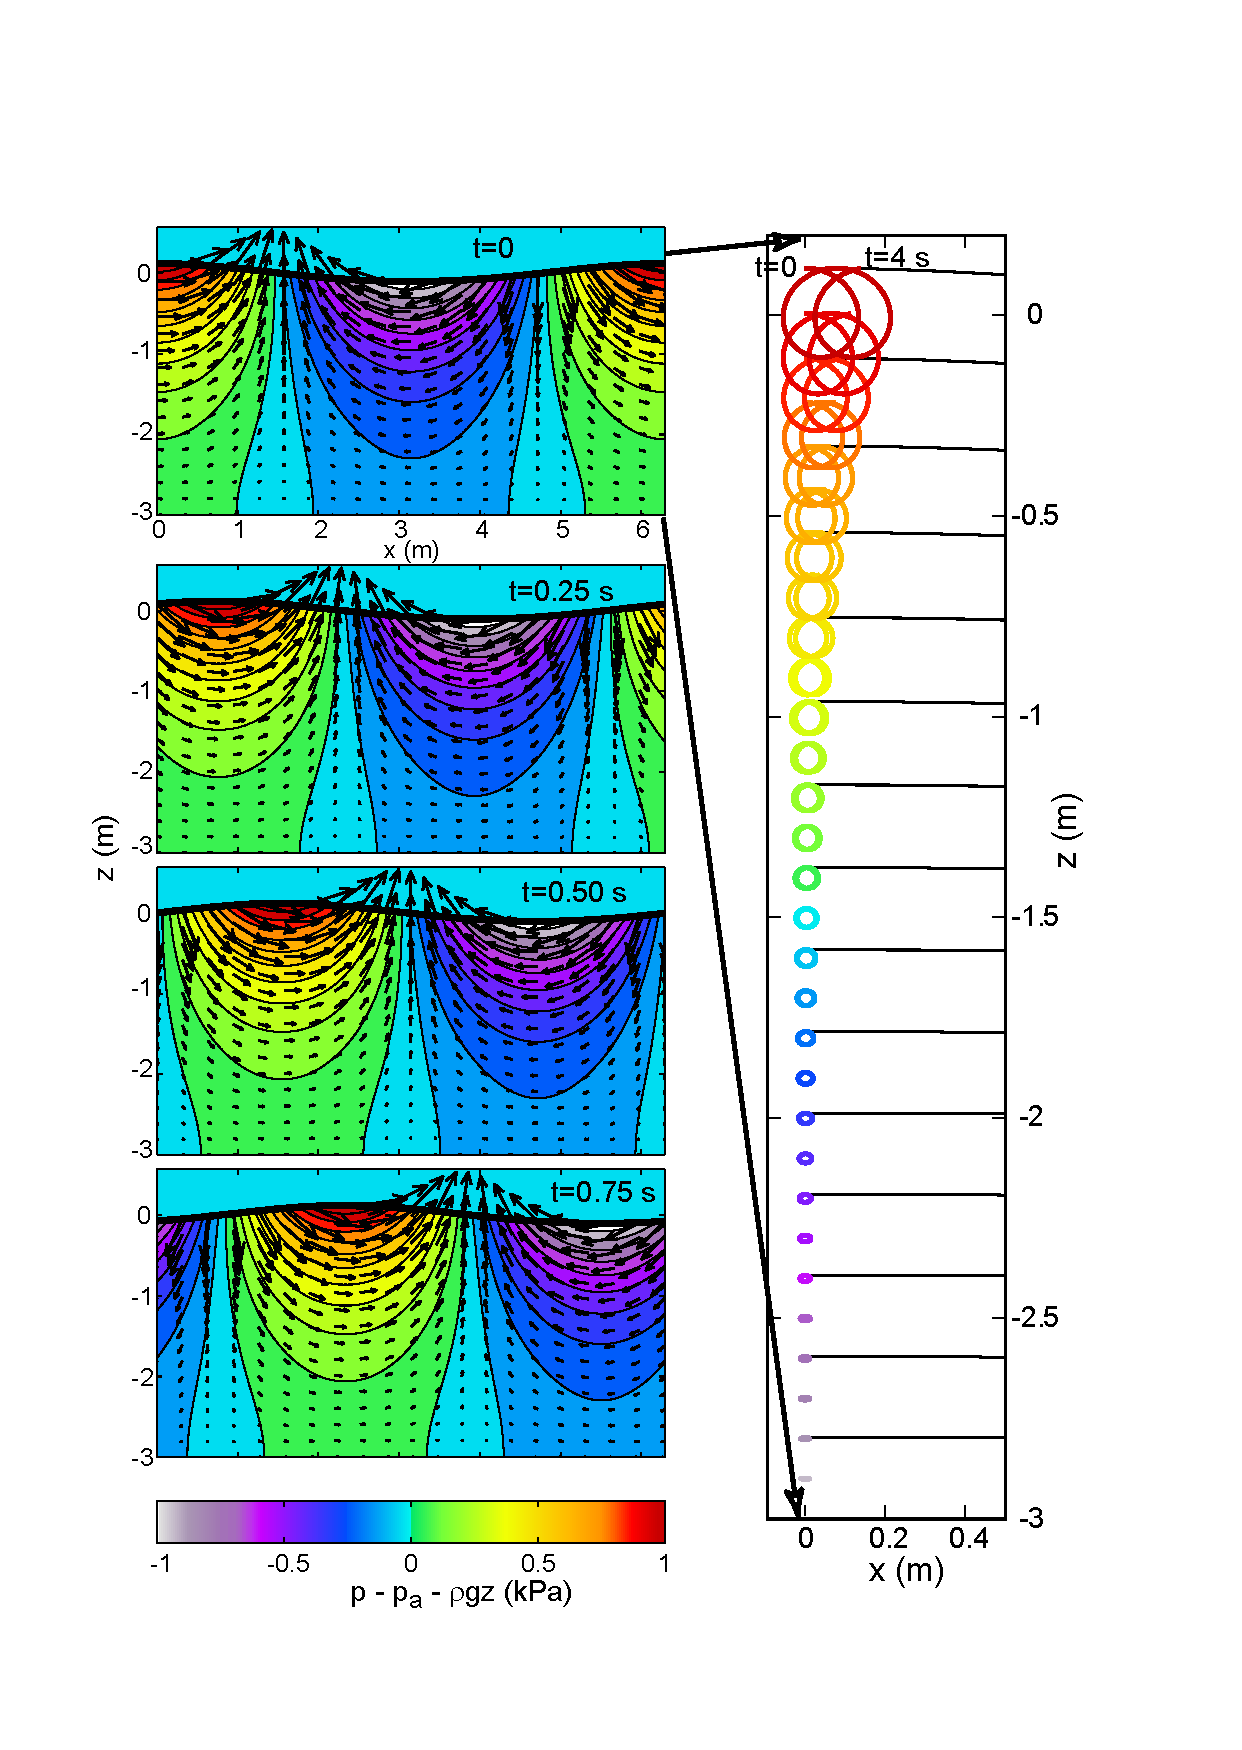
\includegraphics[width=0.9\textwidth]{FIGS_CH_AIRY/2sec_3mdepth_puv_drift.pdf}}
%\vspace{3.64in}
  \caption{Left, in colors: pressure anomaly $p-p^H$ and velocities at different phases 
of the propagation of 2~s period wave in 3~m water depth, going from left to right. 
Right: trajectories of water particles.}
\label{fig:puvdrift}
\end{figure}
%%%%%%%%%%%%%%%%%%%%%%%%%%%%%%%%%%%%%%%%%%%%%%%%%%%%%%%%%%%%%%%%%%%%%%%%%%%%%



%%%%%%%%%%%%%%%%%%%%%%%%%%%%%%%%%%%%%%%%%%%%%%%%%%%%%%%%%%%%%%%%%%%%%%%%%%%%%
\begin{figure}
\centerline{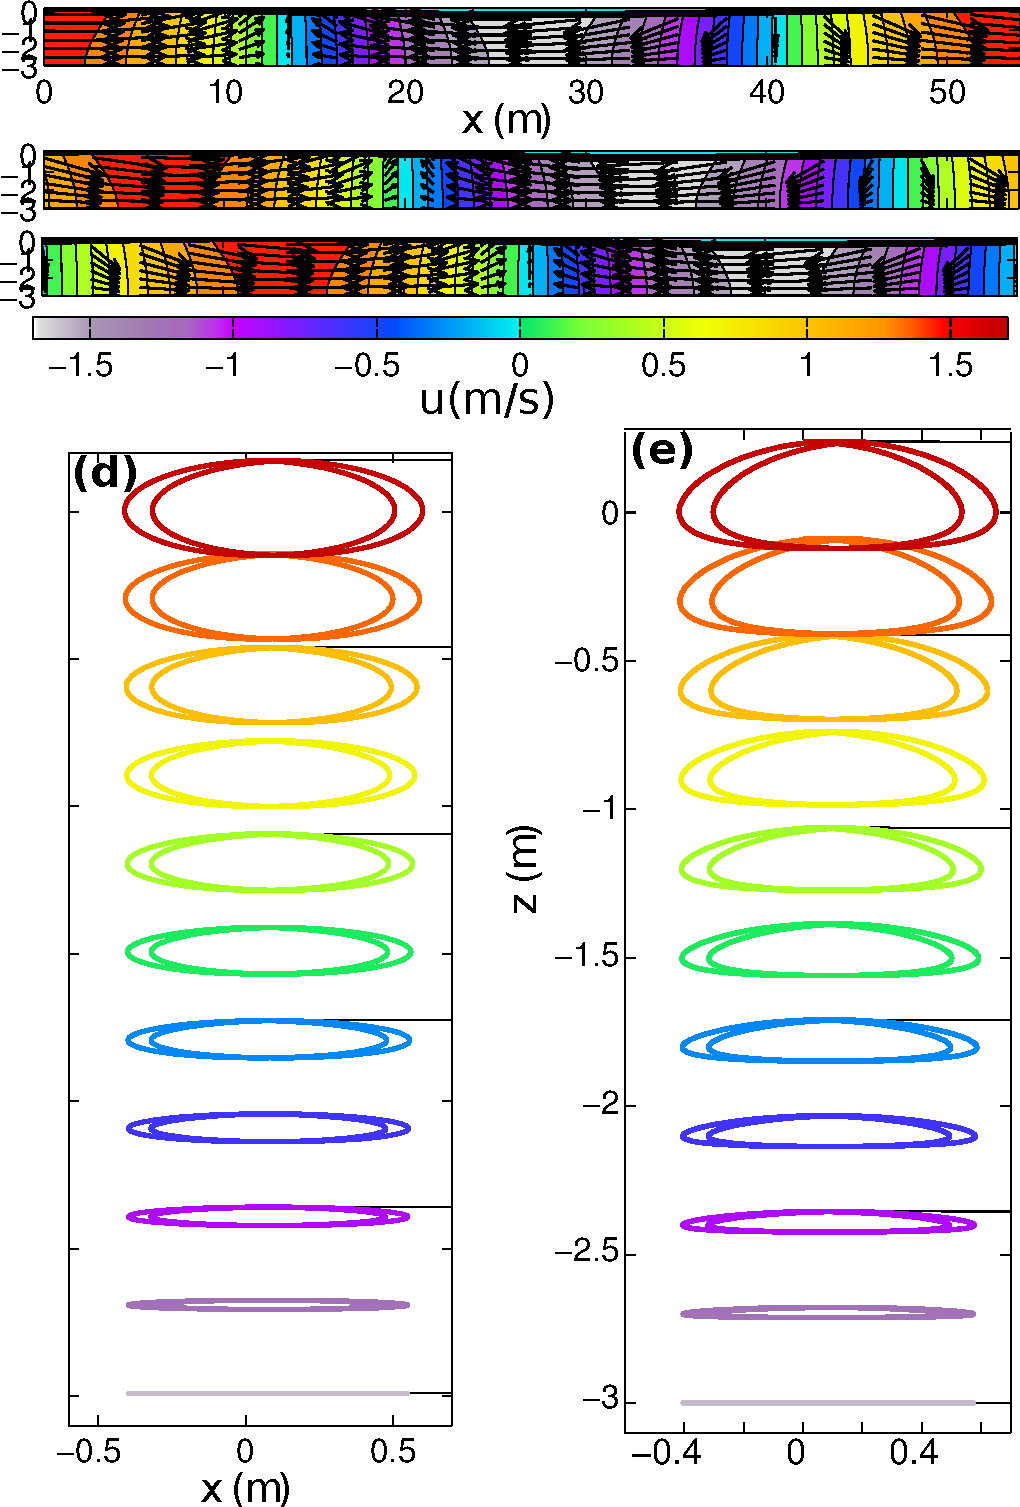
\includegraphics[width=0.7\textwidth]{FIGS_CH_AIRY/10sec_3mdepth_puv_drift.pdf}}
%\vspace{3.64in}
  \caption{Velocity field in water for a wave train of period 10~s, and amplitude 18~cm in 3~m of water. Snapshots are shown for 
(a) $T=0$, (b) 1.25 and (c) 2.5~s. 
The trajectories of water parcels are integrated over two Eulerian periods  (20~s) for (d) linear waves, and (e) nonlinear waves with the 
same period and height, using streamfunction theory (see part 3). For the height chosen here, $H/D=0.12$ and $H/L=0.0067$, so that 
linear theory gives a  fairly good approximation. }
\label{fig:uv2}
\end{figure}
%%%%%%%%%%%%%%%%%%%%%%%%%%%%%%%%%%%%%%%%%%%%%%%%%%%%%%%%%%%%%%%%%%%%%%%%%%%%%



\subsection{Kinematics: influence of the non-dimensional depth $kD$}
The changes in kinematics and dispersion from deep to shallow water are related to the hyperbolic functions $\cosh$, $\sinh$
and $\tanh$, which are plotted in figure \ref{coshsinh}.
%%%%%%%%%%%%%%%%%%%%%%%%%%%%%%%%%%%%%%%%%%%%%%%%%%%%%%%%%%%%%%%%%%%%%%%%%%%%%
\begin{figure}
\centerline{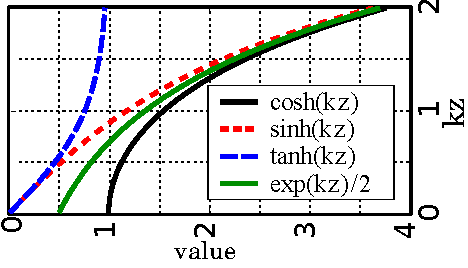
\includegraphics[width=0.5\textwidth]{FIGS_CH_AIRY/coshsinh_en.pdf}}
%\vspace{3.64in}
  \caption{The main hyperbolic functions, used again and again in ocean wave theory.}
\label{coshsinh}
\end{figure}
%%%%%%%%%%%%%%%%%%%%%%%%%%%%%%%%%%%%%%%%%%%%%%%%%%%%%%%%%%%%%%%%%%%%%%%%%%%%%


\subsubsection{Airy waves in deep water}
 A good number to remember is that, at a depth equal to half the
wavelength,  the motion amplitude is reduced by a factor $\exp(\pi) \simeq 25$ compared to the value at the surface.
As a result, waves such that $D > L/2$ which corresponds to $kD > \pi$, are generally considered to be 'deep water waves'.

The dispersion relation becomes, 
\begin{equation}
    \sigma^2 \simeq g k,
     \label{dispersion deep}
\end{equation}
the orbital velocities and pressures become
\begin{equation}
    \ub=a{\mathbf k}\frac{\sigma}{k}
    {\mathrm e}^{kz}    \cos \Theta
\end{equation}
\begin{equation}
    w=a \sigma
    {\mathrm e}^{kz}    \sin \Theta.
\end{equation}
\begin{equation}
    p=\overline{p}^H+ \rho_w g a
    {\mathrm e}^{kz}    \cos \Theta.
\end{equation}
and displacements (\ref{xi1})-(\ref{xi3}) are now
\begin{equation}
    \widetilde{\xi}_h=-a \frac{\mathbf k}{k}
    {\mathrm e}^{kz}  \sin \Theta,
\end{equation}
\begin{equation}
    \widetilde{\xi}_3= a {\mathrm e}^{kz}  \cos \Theta,
\end{equation}
which is the parametric equation of a circle of radius $a {\mathrm e}^{kz}$.
In first approximation, the water parcels follow circular orbits with diameters that vanish with deph. 
 
\subsubsection{Airy waves in intermediate water depth}
For smaller water depths, the orbital velocity is significant near the bottom 
and the trajectories are now ellipses with horizontal major axis measuring 
$2 a
{\cosh\left(kz+kh\right)}/{\sinh\left(kD\right)}$, and 
a vertical minor axis $2 a
{\sinh\left(kz+kh\right)}/{\sinh\left(kD\right)}$ that shrinks from $2a$ at the surface, 
to zero at the bottom where the motion is back and forth along the 
bottom.

In that range there is no asymptotic expression for the dispersion relation and one may use Table \ref{table_dispersion}. 

%%%%%%%%%%%%%%%%%%%%%%%%%%%%%%%%%%%%%%%%%
\begin{table}
  \centering
  \begin{tabular}{|cc  | cc | cc|}
\hline
    $Y=X\tanh(X)$ & $X$     & $Y=X\tanh(X)$ & $X$   & $Y=X\tanh(X)$ & $X$\\
 \hline
       0.05    &     0.2255   &     1.05 & 1.2414 &     2.05 & 2.1110	\\
       0.10    &     0.3216   &     1.10 & 1.2831 &     2.10 & 2.1570	\\
       0.15    &     0.3973   &     1.15 & 1.3249 &     2.15 & 2.2031	\\
       0.20    &     0.4627   &     1.20 & 1.3668 &     2.20 & 2.2495	\\
       0.25    &     0.5218   &     1.25 & 1.4088 &     2.25 & 2.2961	\\
       0.30    &     0.5767   &     1.30 & 1.4511 &     2.30 & 2.3428	\\
       0.35    &     0.6284   &     1.35 & 1.4934 &     2.35 & 2.3898	\\
       0.40    &     0.6778   &     1.40 & 1.5360 &     2.40 & 2.4370	\\
       0.45    &     0.7255   &     1.45 & 1.5788 &	2.45 & 2.4843	\\
       0.50    &     0.7717   &     1.50 & 1.6218 &	2.50 & 2.5318	\\
       0.55    &     0.8168   &     1.55 & 1.6651 &	2.55  &      2.5795   \\
       0.60    &     0.8611   &     1.60 & 1.7085 &	2.60  &      2.6273   \\
       0.65    &     0.9046   &     1.65 & 1.7523 &	2.65  &      2.6753   \\
       0.70    &     0.9476   &     1.70 & 1.7962 &	2.70  &      2.7234   \\
       0.75    &     0.9902   &     1.75 & 1.8405 &	2.75  &      2.7716   \\
       0.80    &     1.0324   &     1.80 & 1.8850 &	2.80  &      2.8200   \\
       0.85    &     1.0744   &     1.85 & 1.9297 &	2.85  &      2.8684   \\
       0.90    &     1.1163   &     1.90 & 1.9747 &	2.90  &      2.9170   \\
       0.95    &     1.1580   &     1.95 & 2.0199 &	2.95  &      2.9657   \\
       1.00    &     1.1997   &     2.00 & 2.0653 &	3.00  &      3.0145   \\
\hline
\end{tabular}
  \caption{Table of the inverse function of $X \tanh X$. Defining $Y=\sigma^2 D/g$ it gives $k=X/D$, 
which allows to invert the dispersion relation in the absence of current. 
For $Y< 0.05$ one should use $X=\sqrt{Y}$, and for $Y >3$ one should use $X=Y$. A more practical alternative is the Padé approxim}\label{table_dispersion}
\end{table}
%%%%%%%%%%%%%%%%%%%%%%%%%%%%%%%%%%%%


\subsubsection{Airy waves in shallow water}
For very shallow water  (say $kD < 0.1$), the dispersion relation 
becomes
\begin{equation}
    \sigma^2=g D  k^2,
     \label{dispersion shallow}
\end{equation}
and the velocities and pressure are 
\begin{equation}
    \ub=a{\mathbf k}\frac{\sigma}{k \sinh(k D)}
        \cos \Theta
\end{equation}
\begin{equation}
    w=a \sigma
    \frac{\left(kz+kh\right)}{\left(kD\right)}    \sin \Theta.
\end{equation}
\begin{equation}
    p=\overline{p}^H+ \rho_w g a     \cos \Theta = p^H.
\end{equation}
This last expression states that the pressure is hydrostatic, just like in 
tidal waves. Tsunamis also nearly follow this shallow water limit. 

 The orbital displacement (\ref{xi1})-(\ref{xi3})
are now
\begin{equation}
    \widetilde{\xi}_h=-a \frac{\mathbf k}{k \sinh(k D)}
    \sin \Theta,
\end{equation}
\begin{equation}
    \widetilde{\xi}_3= a \frac{\left(kz+kh\right)}{\left(kD\right)}  \cos \Theta,
\end{equation}

\subsection{And in the air?}
So far we have solved for the water motion. The same hypotheses of irrotational 
and incompressible flow will, in the air, produce the same equations and solutions. 
The only difference is that the bottom boundary condition is replaced by 
${\mathbf u}\rightarrow0$ as $z\rightarrow\infty$.
The air motion over waves is thus similar to the water motion in deep water waves. 
The air pressure oscillates, with an amplitude that decays exponentially 
with elevation. 
%%%%%%%%%%%%%%%%%%%%%%%%%%%%%%%%%%%%%%%%%%%%%%%%%%%%%%%%%%%%%%%%%%%%%%%%%%%%%
\begin{figure}
\centerline{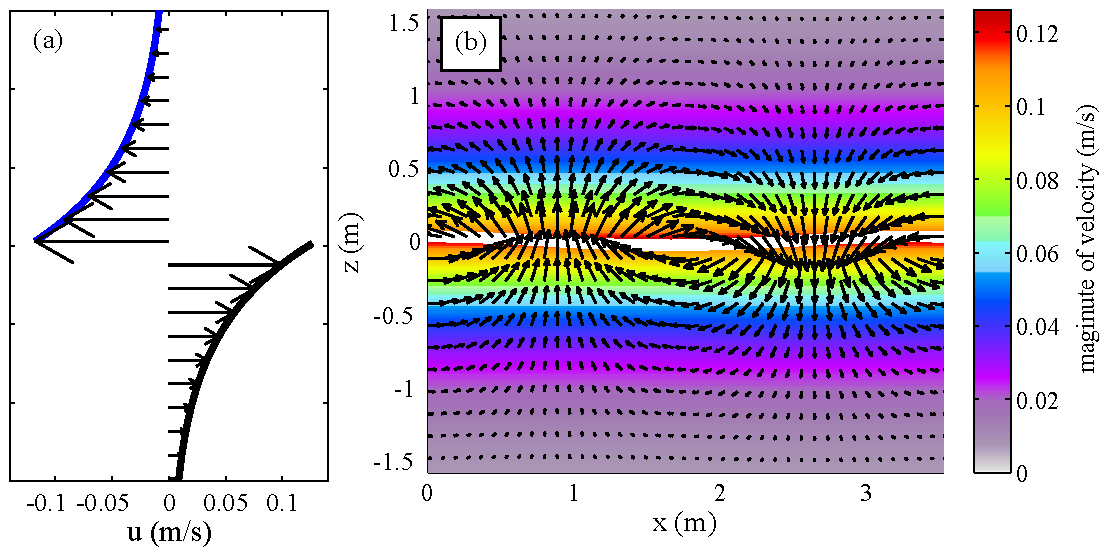
\includegraphics[width=\textwidth]{FIGS_CH_AIRY/vitesse_air_eau_en.pdf}}
%\vspace{3.64in}
  \caption{(a) Profile of the horizontal and vertical velocities on both sides 
of the sea surface at a wave crest ($x=0$), and (b) velocity field, with the white line indicating 
the position of the free surface. These velocities correspond to waves of amplitude $a=3$~cm, 
period $T=1.5$~s, in $D=3$~m water depth, which correspond to a wavelength 
$L=3.5$~m, and a non-dimensional water depth $kD=3.4$. }
\label{vitesse_air_eau}
\end{figure}
%%%%%%%%%%%%%%%%%%%%%%%%%%%%%%%%%%%%%%%%%%%%%%%%%%%%%%%%%%%%%%%%%%%%%%%%%%%%%

These results were confirmed by the measurements of \cite{Elliott1972a}, who 
found a vertical decay that is slightly faster than $\mathrm{e}^{-kz}$, due to 
the effect of the mean shear in the wind speed. When this shear is taken into account, the
Laplace equation is replaced by the Orr-Sommerfeld equation, as detailed in Part 3.
Besides, the velocity jump at the air-sea interface, gives rise to a boundary layer 
that is laminar for low wave heights and wind speeds \citep{Dore1978}, but becomes turbulent 
otherwise \citep{Perignon&al.2014}, probably leading to an important dissipation of long waves traveling across oceans that is 
discussed in Part 3.

\subsection{Dispersion}
The velocity at which the wave crests or trough propagate 
is called the phase speed and is given by $C=\sigma/k$ which is also equal to the ratio $L/T$. 
Using the dispersion relation (\ref{dispersion}), we can eliminate $\sigma$
\begin{equation}
    C= \frac{\sigma}{k}=\left[ \frac{g}{k}\tanh \left( kD\right)\right]^{1/2}.
\end{equation}
The phase speed is clearly a function of the wavelength, and thus waves are 
dispersive, meaning that wave packets that contain different components will 
spread over a larger space as they propagate, with the long waves traveling 
faster than the shorter waves. As a result, the waves arriving from a distant storm will 
always have a long period at the beginning and the average period will become shorter over time. 

This dispersion property disappears in shallow water  ($ kD << 1$)
where $C$ goes to $\left( gD\right)^{1/2}$, independently of $k$.
On figure \ref{disperlinLT}, this gives a constant slope, for example for $D=10$~m and $T>5$~s).
%%%%%%%%%%%%%%%%%%%%%%%%%%%%%%%%%%%%%%%%%%%%%%%%%%%%%%%%%%%%%%%%%%%%%%%%%%%%%
\begin{figure}
\centerline{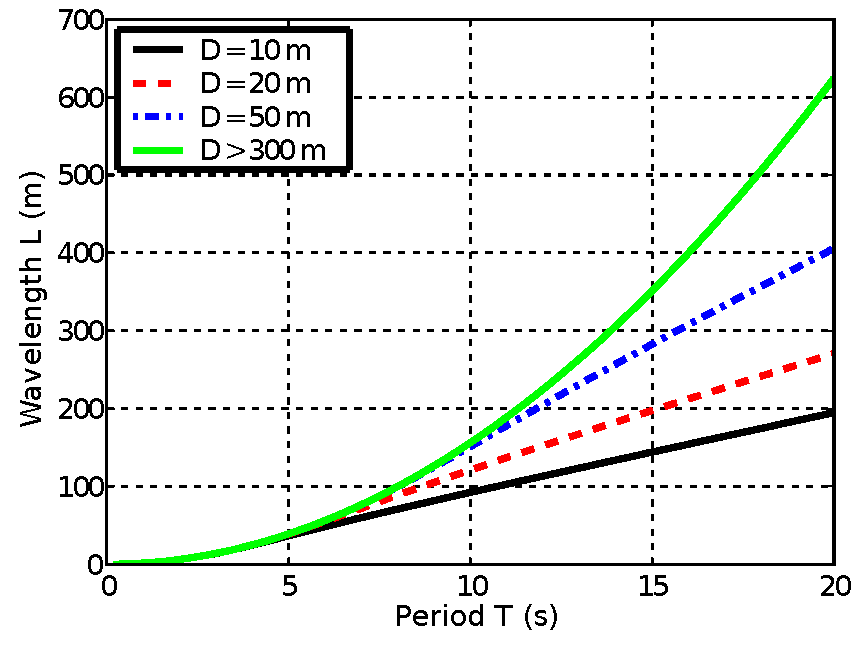
\includegraphics[width=0.8\textwidth]{FIGS_CH_AIRY/disperlinLT_en.pdf}}
%\vspace{3.64in}
  \caption{Wavelength as a function of the wave period and the water depth $D$, for linear waves in the 
absence of currents.}
\label{disperlinLT}
\end{figure}
%%%%%%%%%%%%%%%%%%%%%%%%%%%%%%%%%%%%%%%%%%%%%%%%%%%%%%%%%%%%%%%%%%%%%%%%%%%%%

We also note that, for a fixed period, the phase speed decreases 
with the water depth. This property is also true for a slowly varying water, 
in which case one can consider that the water depth is 'locally constant'. 
This variation of $C$ is the cause of refraction (see chapters \ref{ch_current} and \ref{ch5}). 


\subsection{Energy}
For any water particle, there is an oscillation of the kinetic and potential energies that are exchanged. 
Once integrated over the water depth and averaged over a wave period, that average is represented here by 
the overbar, the potential energy per unit horizontal surface is the vertical integral 
of the potential energy per unit volume $ \rho_w g z$. In practice, we ignore the constant energy between the 
bottom and the mean sea level $\overline{\zeta}$, and we set our reference level such that $\overline{\zeta}=0$,
\begin{eqnarray}
    E_p & = & \overline{ \int_{0}^{\zeta\left(\mathbf{x},t\right)} \rho_w g z {\mathrm d}z }
          = \rho_w g  \overline{ \frac{1}{2} \left(\zeta\right)^2 }   \nonumber\\
    & = & \frac{1}{2} \rho_w g a^2 \overline{ \cos^2\left({\mathbf k} \bcdot {\mathbf x}
    - \sigma t \right) } \nonumber\\
    & = & \frac{1}{4} \rho_w g a^2.
\end{eqnarray}
For the kinetic energy we integrate the kinetic energy per unit volume, $\left( \left|{\mathbf u}\right|^2 + w^2 \right)$ to obtain 
a kinetic energy per unit horizontal surface, 
\begin{eqnarray}
    E_c & = & \overline{  \int_{-h}^{\zeta\left(\mathbf{x},t\right)} \frac{1}{2} \rho_w
\left( \left|{\mathbf u}\right|^2 + w^2 \right) {\mathrm d}z } \nonumber\\
    & \approx & \frac{1}{2} \rho_w \left( \frac{a g k}{\sigma \cosh \left( kD \right)}
    \right)^2 \left[  \overline{ \cos^2 \Theta } \int_{-h}^{\zb} \cosh^2\left(kz+kh\right) {\mathrm d}z 
                   + \overline{ \sin^2 \Theta } \int_{-h}^{\zb} \sinh^2\left(kz+kh\right) {\mathrm d}z     \right] \nonumber\\
    & \approx & \frac{1}{4} \rho_w \left( \frac{a g k}{\sigma \cosh \left( kD \right)}
    \right)^2 \int_{-h}^{\zb} \cosh\left(2kz+2kh\right) {\mathrm d}z \nonumber \\
    & \approx & \frac{1}{4} \rho_w \left( \frac{a g k}{\sigma \cosh \left( kD \right)}
    \right)^2 \frac{\sinh 2kD}{2k}  \nonumber \\
    & \approx & \frac{1}{4} \rho_w g a^2,
\end{eqnarray}
\begin{equation}
    E_t= E_c+E_p= \frac{1}{2} \rho_w g a^2 = \rho_w g  E  ,\label{Etot}
\end{equation}
where $E$ is the variance of the sea surface elevation, here $E=a^2 /2$. 
We have thus found that, to a first order of approximation, the average kinetic and potential energy 
 $E_c$ and $E_p$ are equal. 

Wave propagation is associated to a flux of energy. This flux of energy is transmitted by pressure forces
from one water column to the next. This flux is the work 
of pressure forces given by eq. (\ref{pression}) with a velocity given by eq. (\ref{vitesse}). 
When integrated over the depth and averaged over a wave period, this gives the flux per unit crest length (i.e. per unit horizontal 
distance in the direction perpendicular to the propagation direction), 
\begin{eqnarray}
    W & = & \overline{ \int_{-h} ^{\zeta} p u \mathrm{d}z } \nonumber \\
        & = & \rho_w g a^2 \sigma
        \overline{ \cos^2\left({\mathbf k} \bcdot {\mathbf x} - \sigma t \right)  }
        \int_{-h} ^{\zeta} \frac{\cosh^2 \left(kz+kh \right)}{\sinh kD \cosh kD}
        ~ \mathrm{d}z \nonumber \\
        & = & E_t \frac{2  \sigma}{\sinh (2 kD)}
        \int_{-h}^{\zb} \frac{1}{2}\left[\cosh \left(2kz+2kh\right) +1 \right]
        \mathrm{d}z \nonumber \\
        & = & E_t \frac{2  \sigma}{\sinh (2 kD)}
        \left(\frac{\sinh 2kD}{4k}+\frac{D}{2} \right) \nonumber \\
        & = & C_g E_t \label{W}
\end{eqnarray}
where
\begin{equation}
C_g=\frac{\sigma}{k}
        \left(\frac{1}{2}+\frac{kD}{\sinh 2kD}\right)= C \left(\frac{1}{2}+\frac{kD}{\sinh 2kD}\right). \label{Cg}
\end{equation}
$W$ is a flux of energy per unit distance and $C_g$ the average speed at which the energy density $E_t$ is radiated, 
which defines the group speed. 

The full expression for the energy flux should also include the advective flux  $u \left[\rho_w g z + 0.5\left(u^2 +
w^2\right) \right]$, but that part is negligible in the absence of currents. 
%%%%%%%%%%%%%%%%%%%%%%%%%%%%%%%%%%%%%%%%%%%%%%%%%%%%%%%%%%%%%%%%%%%%%%%%%%%%%
\begin{figure}[htb]
\centerline{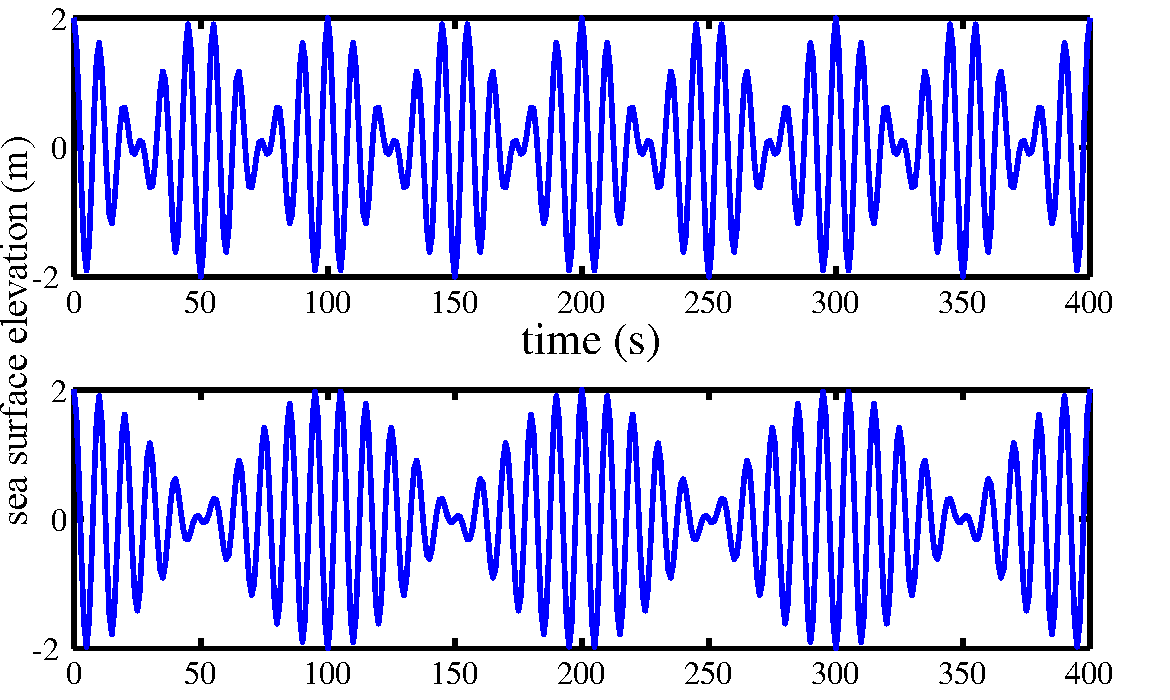
\includegraphics[width=0.7\textwidth]{FIGS_CH_AIRY/groups_5_10_en.pdf}}
%\vspace{3.64in}
  \caption{Wave groups produced by the superposition of two monochromatic waves. The top panel corresponds to  $\Delta \sigma/\sigma=0.2$, and the bottom panel
 $\Delta \sigma/\sigma=0.1$. The narrower the spectrum, the larger the number of waves in the group.}
\label{groupes}
\end{figure}
%%%%%%%%%%%%%%%%%%%%%%%%%%%%%%%%%%%%%%%%%%%%%%%%%%%%%%%%%%%%%%%%%%%%%%%%%%%%%

%%%%%%%%%%%%%%%%%%%%%%%%%%%%%%%%%%%%%%%%%%%%%%%%%%%%%%%%%%%%%%%%%%%%%%%%%%%%%
\begin{figure}
\centerline{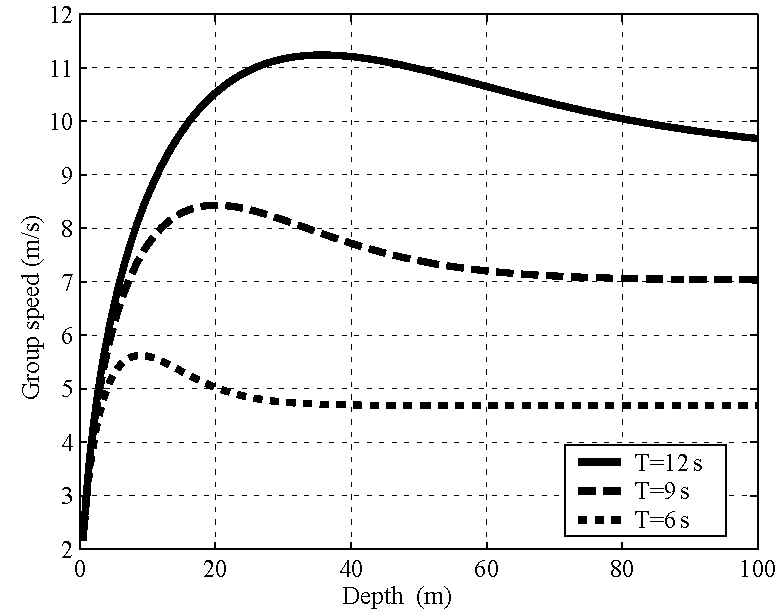
\includegraphics[width=0.55\textwidth]{FIGS_CH_AIRY/cg_en.pdf}}
%\vspace{3.64in}
  \caption{Group speed variation for different periods, as a function of the water depth.}
\label{Cgplot}
\end{figure}
%%%%%%%%%%%%%%%%%%%%%%%%%%%%%%%%%%%%%%%%%%%%%%%%%%%%%%%%%%%%%%%%%%%%%%%%%%%%%

This speed is called 'group speed' because it is indeed the speed at which a group of waves travels, because $C_g=\partial
\sigma/\partial k$. Indeed, the superposition of two monochromatic waves of equal amplitude and similar frequencies gives a surface elevation 
\begin{equation}
    \zeta=a  \cos \left[ \left(k - \Delta k \right) x - \left(\sigma-\Delta \sigma \right) t \right]
        + a  \cos \left[ \left(k + \Delta k \right) x - \left(\sigma+\Delta \sigma \right) t\right]  ,
\end{equation}
which writes
\begin{equation}
    \zeta=2 a \cos \left(\Delta k x -\Delta \sigma t\right)
    \cos \left( k x - \sigma t\right).
\end{equation}
The first factor is the envelope of the group, with a length  $2 \pi /
\Delta k $ and period $2\pi / \Delta \sigma$, that propagates at the speed 
$c'=\Delta \sigma /\Delta k $. This speed is, in the limit  $\Delta k \rightarrow 0$, equal to 
$C_g=\partial \sigma/\partial k$. Two examples are shown in figure 
\ref{groupes}.


We note that for $kD\rightarrow\infty$, equation (\ref{Cg}) gives
$C_g={\sigma}/({2k})=C/2$. Thus, in deep water the groups of waves travel at a speed that is half of the phase speed. 
Things are very different in shallow water ($kD
\ll 1$), where $C_g=C$. In that shallow water limit, waves of all frequencies travel at the same speed (they are not dispersive)
hence the groups also travel at that same speed. This is only true for linear waves. In part 3you may see that  phase and group speeds 
are also a function of the wave amplitude. 


\subsection{Energy and power}
Eq. (\ref{W}) gives the mean energy flux per unit crest length. 
For example, in the case of monochromatic waves with a height of 2~m, a period of 12~s and
a water depth of 15~m, this flux is 
$W\approx 50$~kW~m$^{-1}$. This means that if we take a surface facing the waves, 1 meter along the crest and the full water depth, there is 50~kW of mechanical power that goes through this surface. 
This is 5~MW for 100~m along the crests, which is the peak power of two  150~m high windmills. This number, for rather modest wave heights, 
shows the strong concentration of power in water waves. Unfortunately, this power is difficult to tap to produce electricity, in particular because it is very intermittent in most places.

\subsection{Summary}
We have obtained the main properties of regular linear waves,  summarized in table 
(\ref{table_theory}). Because these Airy waves are solutions of the linearized equations of motion, 
they can be combined to obtain the general solution. Hence the surface elevation, velocities and pressure 
are given by the sum of monochromatic waves, each proportional to their amplitude $a$. We will see in the next chapter that it is also possible to add up the quadratic properties 
that are the energy and Stokes drift, which are  proportional to the surface elevation variance
$E=a^2/2$.
%%%%%%%%%%%%%%%%%%%%%%%%%%%%%%%%%%%%%%%%%%%
\begin{table}
  \centering
  \begin{tabular}{lccc}
\hline
  Water depth: & general case       & $kD \gg 1$  & $kD \ll 1$  \\
\hline
  dispersion relation  &   $\sigma^2=g k \tanh (kD)  $               & $ \sigma^2=g k$ & $\sigma^2=g D k^2 $ \\
  phase speed & $C= {\sigma}/{k}=\left[g  \tanh (kD)/ k\right]^{1/2}$         & $C=\left(g / k\right)^{1/2} ={g}/{\sigma}  $   & $ C = \sqrt{gD}^{1/2}$ \\
  group speed  &  $C_g=C \left(0.5+\frac{kD}{\sinh(2kD)}\right)  $               & $C_g=C/2 $&
  $C_g=C$\\
\hline
  Linear properties  ($z<\zeta$) &    &  & \\
\hline
  horizontal velocity & $\ub =   a \frac{{\mathbf k}}{k}\sigma
    \frac{\cosh\left(kz+kh\right)}{\sinh\left(kD\right)}
    \cos \Theta $         &  $\ub=\frac{a \kb \sigma}{k} \er^{kz}    \cos \Theta$ & $\ub=\frac{a \kb \sigma}{k^2 D}
        \cos \Theta $\\
  vertical velocity & $w =   a \sigma
    \frac{\sinh\left(kz+kh\right)}{\sinh\left(kD\right)}
    \sin \Theta $         &  $w =a \sigma \er^{kz}    \sin \Theta$ & $w=\frac{z+h}{h}{a \sigma} \sin \Theta $\\
\hline
  Quadratic properties &    &  & \\
\hline
 Mean energy per unit surface & $E_t =  \rho_w g E = \rho_w g a^2 /2$  & $E_t =  \rho_w g  a^2 /2$ & $E_t =  \rho_w g  a^2 /2$ \\
 Stokes drift & ${\mathbf U}_s=\sigma \kb E \frac{\cosh(2kz+2kh)}{\sinh^2(kD)}$  & ${\mathbf U}_s=2 \sigma \kb E \er^{2kz} $ & ${\mathbf U}_s=\sigma \kb E /(kD)^2$ \\
\hline
\end{tabular}
  \caption{Main results of Airy wave theory with deep and shallow water limites.  We remind that the phase is  $\Theta={\mathbf
k}\bcdot{\mathbf x}-\sigma t+ \Theta_0$.
}\label{table_theory}
\end{table}
%%%%%%%%%%%%%%%%%%%%%%%%%%%%%%%%%%%%
These properties come from a series of assumptions, listed in table \ref{table_H} and that will be discussed or removed in 
the following chapters that extend Airy theory, giving access to all sorts of corrections and allowing to determine the 
evolution of Airy waves caused by different forcing and dissipation processes. Indeed, we have determined here the 
eigenvectors of the linearized equations of motion: these are free waves that can exist without forcing. In practice, the forcing 
is necessary to generate these waves in the first place, and this forcing is balanced by dissipation when long time scales and large 
spatial scales are considered. That dissipation requires to include vorticity and viscous effects. 
%%%%%%%%%%%%%%%%%%%%%%%%%%%%%%%%%%%%%%%%%%%
\begin{table}
  \centering
  \begin{tabular}{lcc}
\hline
 Assumption          & justification                                  & consequences  \\
\hline
 A1. incompressible &   $u \ll \alpha_w $             & $\bnabla \bcdot \ub + \partial w/\partial z=0$ \\
 A2. rigid bottom   & bottom motion $\ll$ water motion & $w=-\ub \bcdot \bnabla h$ at $z=-h$ \\
 A3. inviscid       & high Reynolds number                    & viscous stresses are zero \\
 A4. irrotational   & motion driven by pressure forces + (A3)   & $\ub=\bnabla \phi$, $w=\partial \phi/\partial z$\\
 A5. flat bottom    & bottom slopes usually $\ll$ 1 & with A2, $w=0$ at $z=-h$ \\
 A6. sine wave      & basis function of the Fourier transform & $\phi(z) \propto
 \cosh(kz+kh)$ \\
 A7. $p_a$ constant on $z=\zeta$ & $\rho_a \ll \rho_w$         &  no wave generation by the wind \\
 A8. no surface tension & $\gamma \ll g/k^2$ for $L \gg 0.1$~m (in clean water) & no capillary waves \\
 A9. $\varepsilon_1=ka \ll 1$ & $\varepsilon_1 <0.44$ for periodic waves & with A10, gives linear equations \\
 A10. $\varepsilon_2=a/D \ll 1$ & because it makes equations simpler & ... but beware for  $kD < 1$! \\
 A11. no mean current & most often $U \ll C$  for dominant waves & simple dispersion  $\sigma^2 = gk \tanh(kD)$ \\
 A12. constant density & $\rho'/\rho_w < 0.03$ for sea water   & no internal waves\\
 A13. no Earth rotation  & $f_3 \ll \sigma $          & \\
 \hline
\end{tabular}
  \caption{Assumptions needed to derive Airy's theory. $ \alpha_w$ is the sound speed in water, of the order of 
1500~m~s$^{-1}$ (in the absence of air bubbles), and $U$ is the mean current velocity. Finally $\rho'$ 
is a scale for density perturbations relative to the mean $\rho_w$, and 
 $\gamma$ is the surface tension, such that $\gamma \rho_w (R_1+R_2)$ is the additional pressure under a surface with radii of 
curvature $R_1$ et $R_2$, counted positive for a surface that is convex on the air-side, e.g. a crest.}\label{table_H}
\end{table}
%%%%%%%%%%%%%%%%%%%%%%%%%%%%%%%%%%%%

\subsection{Extending Airy wave theory}
What happens when we do not make one of the assumptions A1 to A13? In which conditions should we do this? 
\begin{itemize}
  \item A1. Except when considering acoustic and seismic noise generated by ocean waves, as in part 3, we can 
safely ignore compressibility effects. \vspace{0.3cm}
  \item A2. Bottom deformations are relevant when considering acoustic and seismic noise generation. In fact, the bottom 
deformation should be considered for all acoustic wave propagation in the ocean.  \vspace{0.3cm}
  \item A3. In the boundary layers at the sea surface, and more importantly at the sea bottom, 
we will need molecular viscosity and turbulence effects (which can often be represented by an eddy viscosity). 
However, these layers are very thin, with a thickness of the order of 
  $\delta=(\nu/\sigma)^{1/2}$, which is typically less than a millimeter for the kinematic viscosity of water 
$\nu \simeq 4\times 10^{-6}$~m$^2$~s$^{-1}$, and wave periods 
   $T > 1$~s, which is consistent with measurements of the water-side surface boundary layer by \cite{Banner&Peirson1998}. At the bottom, 
turbulence effects are important but the wave boundary layer is only a few centimeters thick.\vspace{0.3cm}
  \item A4. For a viscous flow, the vorticity from the top and bottom boundary layers diffuses in the water column 
and in the air \citep{Longuet-Higgins1953,Weber&Forland1990}. Besides, there is also a weak vorticity caused by the 
Earth rotation, see A13 below. \vspace{0.3cm}
  \item A5. The bottom boundary condition becomes $-\bnabla \phi \bcdot \bnabla h = \partial \phi/\partial z$ (inviscid case), 
and is only satisfied exactly in the presence of at least two wave trains, one incident and one reflected. The incident wave train 
is also modified by diffraction effects.
  For small slopes, diffraction and reflection are generally weak, 
and the wave motion is well approximated by a "WKBJ" approximation: replacing the phase  $\Theta$ by a function  $S(\xb,t)$ 
with $\kb=\bnabla S$ and $\sigma=-\partial S/\partial t$ (see chapter 
  \ref{ch5}). In this context \emph{small} means that refraction or diffraction effects do not produce of significant variation 
of the wave amplitude at the scale of one wavelength. A more accurate approximation of the dispersion relation 
over a sloping bottom was given by 
   \cite{Ehrenmark2005}, in the form 
   $\sigma^2=gk \tanh(kh \beta /\tan \beta)$, where $\beta$ is the angle between the bottom and the horizontal. This correction is 
weak, only 4\% for a slope $\beta=10^\circ$. For steep slopes, reflection becomes important and the separation of the 
variables $\xb$ and $z$ becomes meaningless. The velocity potential can be obtained numerically 
  \citep[e.g.][]{Athanassoulis&Belibassakis1999,Belibassakis&al.2001}.\vspace{0.3cm}
  \item A6. For a flat bottom this is not an assumption: we have the right to decompose the waves into sine waves because these 
are a complete basis. For small bottom slopes, the wave train is only \emph{locally} equivalent to a sine wave. 
For steep slopes, the wave train can suffer strong distortions at the scale of one wavelength \citep[e.g.][]{Magne&al.2007}.\vspace{0.3cm}
  \item A7. An atmospheric pressure oscillation on the scale of the wavelength can produce an amplification or attenuation of the waves, depending 
on its phase relative to the waves. This aspect is discussed in detail in chapters \ref{ch_sourceterms} and Part 3. \vspace{0.3cm}
  \item A8. Due to surface tension, the pressure under the surface is increased by  $-\gamma \left(\partial^2 \zeta/\partial x^2+\partial^2 \zeta/\partial
  y^2\right)$. This added pressure modifies the dispersion relation to give $\sigma^2=\left(gk+\gamma k^3\right) \tanh(kD)$. 
  This modification is negligible for wavelengths larger than a few centimeters. The presence of a layer of ice at the sea surface 
has a similar effect on the waves, with added terms due to bending and inertia, and is significant for periods of 10~s and 
less \citep{Liu&MolloChristensen1988} in the case of an ice layer thickness of one meter or more, and  thicker layers have an influence on longer waves.
  \item A9. Non-linear effects associated to $\varepsilon_1 \neq 0$ are fairly complex and will be 
discussed in chapters \ref{ch_sourceterms} and part 3. 
One particular consequence is that a monochromatic wave train is generally 
unstable \citep{Benjamin&Feir1967}. For waves in one dimension, as produced in the laboratory, 
this can create very high (freak) waves. Another consequence is that different wave trains interact, 
exchanging energy an momentum.\vspace{0.3cm}
 \item A10. Non-linear effects associated to  $\varepsilon_2 \neq 0$ are important for $kD<1$ even if the wave height is small. 
This is particularly true near the shoreline, and the shape of waves can be strongly modified, as discussed in chapters \ref{ch_surf} and 
part 3.\vspace{0.3cm}
 \item A11. Since the laws of physics are unchanged by a change of Galilean reference frame, 
a uniform current $\Ub$ in the absence of bottom friction only introduces a Doppler frequency shift, 
and all results established here remain valid, replacing 
$\Theta$ by $\Theta_D=\Theta+\kb \bcdot
 \Ub$. One can define an absolute frequency, as measured in the reference frame attached to the bottom, 
 \begin{equation}
    \omega=\sigma+\kb \bcdot \Ub =\kb \bcdot \Ub + \left[g k \tanh\left(kD\right)\right]^{1/2}.
     \label{dispersionD}
\end{equation}
For a current   $\Ub(z)$ that varies only in the vertical, and in the limit  $\varepsilon_1 \ll 1$  and $\varepsilon_2 \ll 1$, 
this dispersion relation generalizes to the form,
 \begin{equation}
    \omega\equiv\sigma+\kb \bcdot \Ub_A      \label{dispersionD2}
\end{equation}
with the advection speed given by \cite{Kirby&Chen1989}, 
 \begin{equation}
 \Ub_A   = \kb \bcdot \int_{-h}^{\zb} \Ub(z) \frac{2  k
\cosh\left[2k(z+h)\right]}{\sinh(2kD)} \dr z. \label{dispersionD3}
\end{equation}
Finally, when $\Ub$ also varies horizontally, the phase speed varies horizontally, so that refraction and diffraction effects 
appear, just like they do on a sloping bottom. These questions are addressed  in  chapter \ref{ch_current}.\vspace{0.3cm}
\item A12. When the ocean is stratified, due to a vertical variation of temperature and/or salinity, the Airy waves are the 'external mode' in a family of waves that also include internal waves. 
Because the equations of motion are weakly nonlinear, these different modes are coupled, with an exchange of energy between surface waves and internal waves 
\citep{Thorpe1966}. This aspect is still relatively unexplored  \citep{Osborne&Burch1980,Kudryavtsev1994}. This stratification can also be due to the 
presence of air bubbles near the surface or sediments near the bottom, with important consequences for the bottom boundary layer and wave dissipation. 
\citep[e.g.][]{Winterwerp2007,Styles&Glenn2000}.\vspace{0.3cm}
\item A13. Taking into account the Earth rotation with a vertical Coriolis parameter $f_3$, a very weak transversal velocity component $v$ appears, 
of the order  $f_3 u /\sigma$ and in phase with $w$.  This transversal component is important for the surface drift current
 \citep{Hasselmann1970,Xu&Bowen1994,Ardhuin&al.2004b,Rascle&Ardhuin2009}. In the case of wind-generated waves, 
  $f_3/\sigma$ is typically of the order of 10$^{-4}$, so that the effect on the wave kinematics and dispersion is not measurable. 
There is also a very weak deviation of the propagation direction of the waves \citep{Backus1962}. This is still true for tsunamis 
which have much larger periods than wind-waves, typically a few minutes up to 30 minutes. Airy wave theory thus also applies to tsunamis, as long as non-linear effects are 
weak. On the contrary, for motions with longer periods, such as tides, the Earth rotation must be taken into account. This is why these waves are called inertia-gravity waves. 
\end{itemize}



\cleardoublepage
\chapter{Wave heights and spectra: theory and measurement}\label{ch2}
A detailed knowledge of the wave motion in any location is often not required, 
one may rather be interested in the evolution of some wave properties on distances 
much larger than the wavelength.  A statistical approach is therefore preferred.
Note also, that even in a wave tank, waves are never strictly monochromatic.

The most common method to represent the random nature of waves is the spectral analysis. 
It owes its success to the dispersive nature of waves (different components travel at different speeds), and it was made practical by the 
development of computer sciences in the 1960s and to the elegant 
Fast Fourier Transform (FFT) algorithm.  Those curious to know how a spectrum can be calculated without a computer can read the amazing account 
of the rotating system  invented by  \cite{Barber&al.1946} with variable speed to read off different spectral components off a wave record printed on paper .

With the Fourier method, a record of wave elevation $\zeta(t)$ is decomposed into 
a superposition of sine waves, each with a particular period. If the record has the three dimensions, $\zeta(x,y,t)$ this decomposition can be 
done in frequency, wavelength and propagation direction. 
The phases of theses sine waves are generally random, namely, the phase of one component 
in one record and the next record are not correlated at all. The only slowly varying quantity 
is the spectral density, defined as the amount of elevation variance per unit spectral bandwidth. 
The procedure can be applied to other variables, not just the elevation: pressure, velocity ... 
This slow variation of the spectrum allows a numerical prediction of ocean wave spectra. 

\section{Frequency spectrum}
The spectral analysis that is applied to wave measurements is fairly different from the harmonic 
analysis which is used for studying tides. Tides are described as a sum of discrete components whose frequencies are very well known as 
they are associated with astronomical motions. For tides we thus have a finite set of frequencies at which the amplitude and phase 
can be determined with great accuracy. Waves are described as a the sum of a 
 many components with energy at \emph{all} frequencies. There is no gap in the wave spectrum, and the phases are completely random, uniformly 
distributed between 0 and $2 \pi$ while the amplitudes 
also have random fluctuations. The result of the spectral analysis is a wave spectrum that describes
the wave energy distribution as a function of frequency. The practical method used to compute wave 
spectra from time series of surface elevation or pressure is detailed in Chapter \ref{ch_anaspec}. 

%%%%%%%%%%%%%%%%%%%%%%%%%%%%%%%%%%%%%%%%%%%%%%%%%%%%%%%  % FIGS_CH_MEASUREMENTS
\begin{figure}[htb]
\centerline{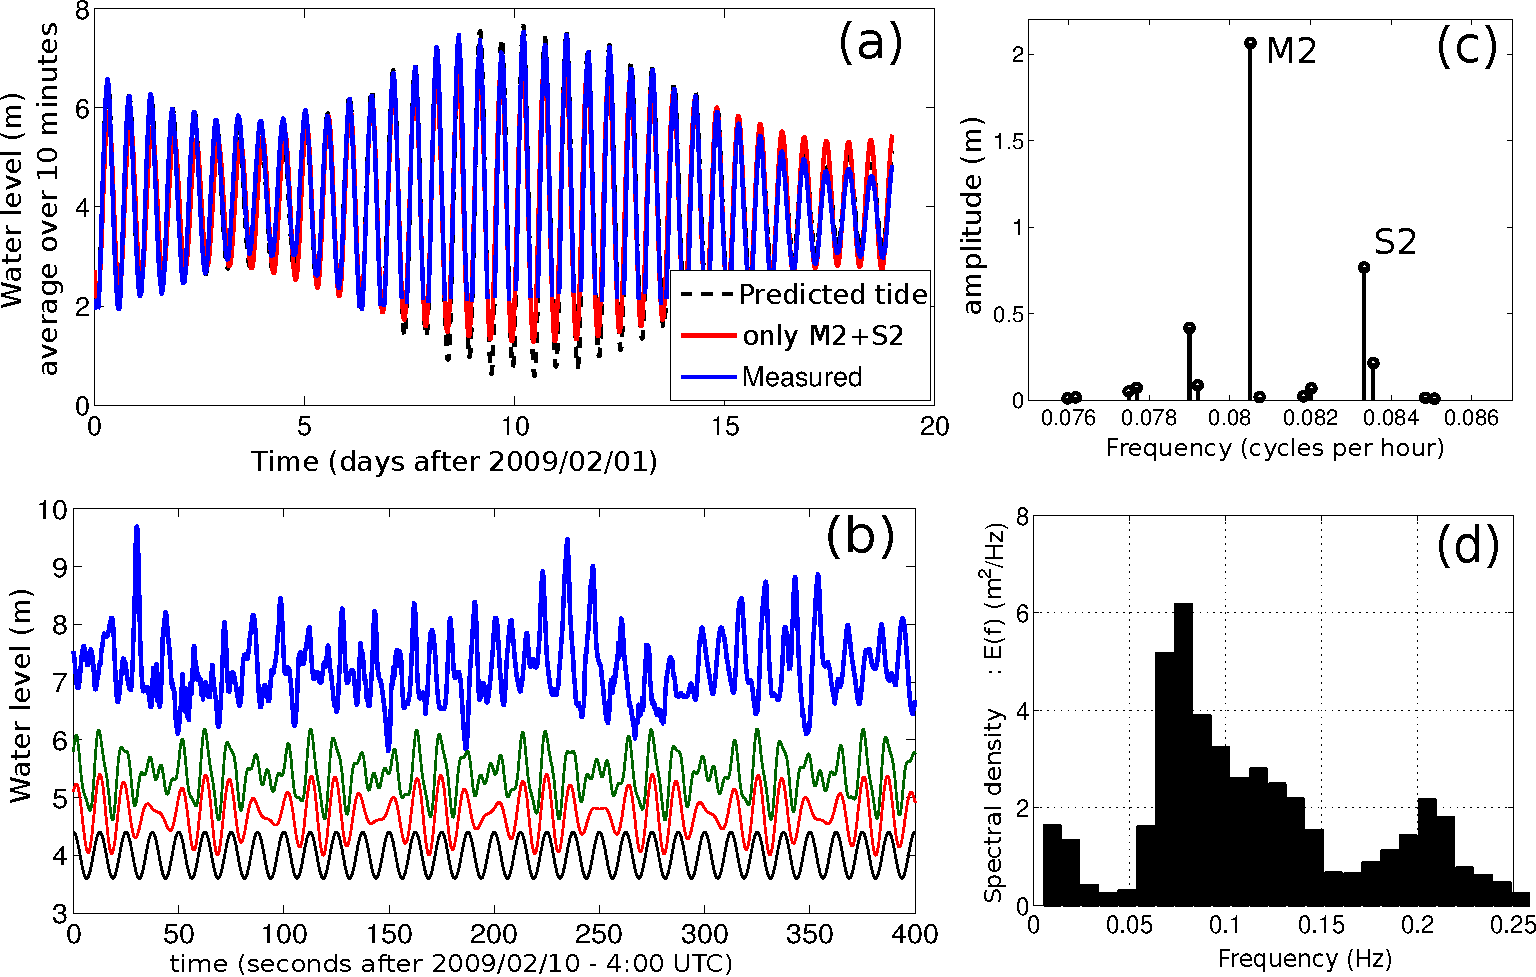
\includegraphics[width=\textwidth]{FIGS_CH_MEASUREMENTS/spectres_maree_vagues_en.pdf}}
%\vspace{3.64in}
  \caption{
Example of  surface elevation time series (a and b) deduced from pressure measurements collected 
as the foot of Western cliff of Banneg Island, Molene Archipelago. The corresponding spectra 
for the high and low frequency part illustrate the difference between a tide spectrum, 
presented as a function of amplitude and a wave spectrum. Below: a sample of the initial 
elevation signal and one, then two, then three sine waves are combined to approximate 
the initial signal. In the case of tides, the fit is already good with 2 components. In the case of 
waves, the detailed shape of the elevation cannot be reproduced without many components.}
\label{fig:maree_vagues}
\end{figure}
%%%%%%%%%%%%%%%%%%%%%%%%%%%%%%%%%%%%%%%%%%%%%%%%%%%%%%%%%%%%%%%%%%%%%%%%%
Figure \ref{fig:maree_vagues} shows how a tide elevation signal is already quite well 
reproduced by the superposition of only two sine waves (these two waves are called S2 and M2). 
On the contrary for the high frequency signal, dominated by waves, one, two or three sines 
waves (black, red and green) are far from sufficient for representing the initial signal (blue). 
Indeed, to reconstruct the wave signal a great number of sine waves with relatively close 
frequencies are required. For simplicity, let us start with one realization $m$ of an elevation 
time series, that can be expressed in terms of a Fourier series,
\begin{equation}
\zeta_{m}(t)=\sum_{i=1}^{N}a_{m,i}\cos(2\pi f_{i}t+ \Theta_{0,m,i})
\label{eq3.1}
\end{equation} 
Where $a_{m,i}$, $f_i$ and $\Theta_{0,m,i}$ are the Fourier amplitudes, frequencies and phases of 
the Fourier mode $i$, found for the realization $m$ of the sea state. As explained above, 
$N$ must be a large number. In practice the phases are nearly random and uniformly 
distributed over [$0,2\pi$] \footnote{The phases are not exactly random for an actual sea state, waves are 
slightly asymmetric, the front face being steeper than the back, and the crests sharper 
than troughs (e.g. \cite{Agnon&al.2005}). For most applications, these effects can be neglected.}. 
The ensemble mean of the Fourier amplitudes, expressed as function of the frequencies, 
 $A(f_i)= \left\langle a_{m,i}\right\rangle$ is called the amplitude spectrum.  For waves, 
identical sea state realizations can only be obtained in controlled laboratory experiments. 
Instead, the sea state is assumed stationary and the ergodicity theorem is evoked to replace the 
ensemble mean by a temporal mean. In practice, $M$ samples of a given (stationary) wave record simulate $M$ 
realizations of the sea state and provide an equivalent ensemble mean. 

For such random signals, the 'power' spectrum is preferred to the amplitude spectrum. 
As demonstrated in the previous chapter, the mechanical wave energy per unit surface of ocean, 
for an sine wave of amplitude $a$ is $\rho_w g a^2/2$. As a consequence, the energy spectrum is
\begin{equation}
\left\langle\frac{1}{2}a_{m,i}^{2}\right\rangle =\frac{1}{M}\sum_{m=1}^{M}\frac{1}{2}a_{m,i}^{2},
\label{eq3.2}
\end{equation}

With this definition, the values taken by the spectrum decrease proportionally to the spectral resolution $\Delta f$ that is the inverse of the length of time 
over which the spectral analysis is performed.  In order to avoid this dependency on the record length, it is customary to work with a power spectral density (PSD for short),
\begin{equation}
E(f_i)=\frac{1}{\Delta f} \left\langle \frac{1}{2} a_{m,i}^{2}\right\rangle. 
\label{eq3.3}
\end{equation}

In the limit of large record lengths, the frequency interval $\Delta f$ tends towards zero, and we obtain the continuous
wave energy frequency spectrum,
\begin{equation}
E(f)=\lim_{\Delta f\to 0}\frac{1}{\Delta f} \left\langle \frac{1}{2} a_{i}^{2}\right\rangle.
\label{eq3.4}
\end{equation}
 
While wave are irregular, the spectrum is relatively smooth, evolving slowly in space and time, with a typical time scale of a few hours. This regularity 
that contrasts with the apparent irregular motion of the sea surface, allows for a predictive numerical modeling. Note further, that
for convenience we continue to call (abusively) 'energy' the elevation variance $E$ which has units of length squared. 
The true energy, in Joules per unit surface, is in fact $\rho_w g E$. 

 This approach can be generalized to waves travelling in all directions. The Fourier representation of the sea surface elevation becomes,  
\begin{equation}
\zeta_m(x,y,t)=\sum_{i=1}^{N} \sum_{j=1}^{M}a_{m,i,j}\cos(2\pi f_{i}t- k_{i}\cos(\theta_{j}) x - k_{i}\sin(\theta_{j}) y + \Theta_{0,m,i,j}),
\label{eq3.5}
\end{equation}
as illustrated by figure \ref{fig:sumofsinewaves}
 %%%%%%%%%%%%%%%%%%%%%%%%%%%%%%%%%%%%%%%%%%%%%%%%%%%%%%%%%%%%%%%%%%%%%%%%%%%%%
\begin{figure}[!htbp]
\centerline{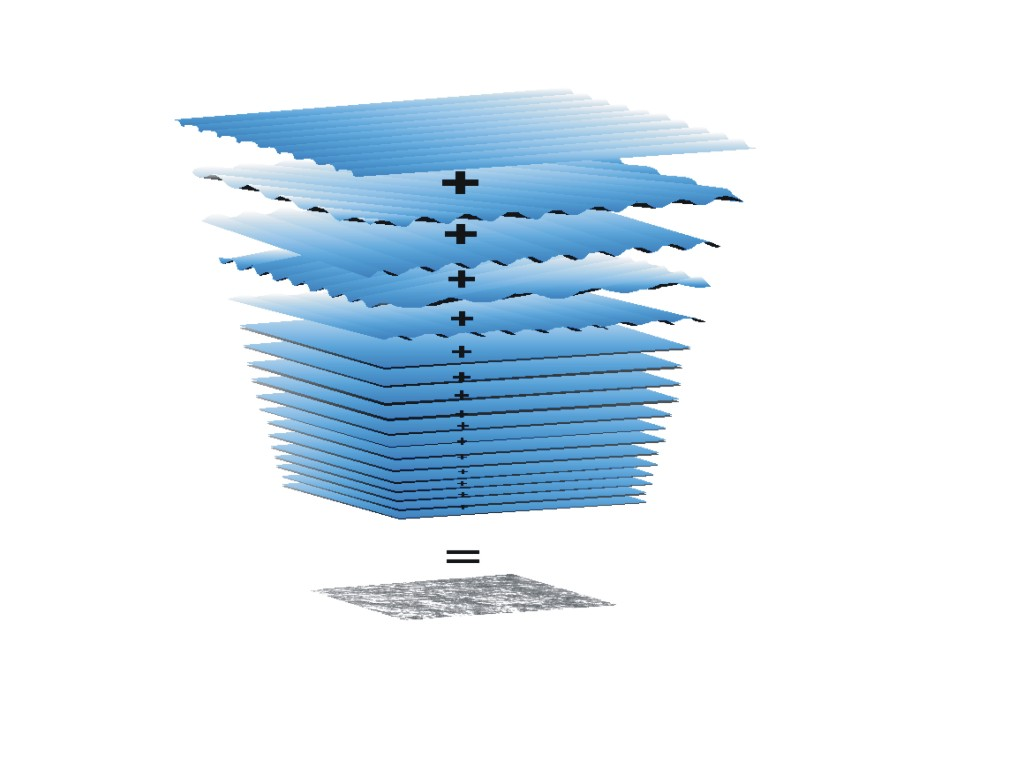
\includegraphics[width=0.8\textwidth]{FIGS_CH_MEASUREMENTS/Pierson1952.jpg}}
\caption{Reconstruction of a given sea state from the superposition of a great number of plane waves each with a particular direction and wavelength. Illustration of equation \ref{eq3.5}. 
After \cite{Pierson&al.1955}.\label{fig:sumofsinewaves}}
\end{figure}
 %%%%%%%%%%%%%%%%%%%%%%%%%%%%%%%%%%%%%%%%%%%%%%%%%%%%%%%%%%%%%%%%%%%%%%%%%%%%%

In this expression $k_{i}$ and $f_i$ are related by the linear dispersion relation and $\theta_{j}$ is the direction of
propagation of the Fourier mode ($i$,$j$). In the same fashion as for the frequency, the continuous frequency-direction wave energy
density spectrum, 
\begin{equation}
E(f,\theta)=\lim_{\Delta f\to 0}\lim_{\Delta \theta\to 0}\frac{1}{\Delta f \Delta \theta} \left\langle \frac{1}{2} \rho_w g a_{i,j}^{2}\right\rangle .
\label{eq3.6}
\end{equation}

Obviously, $E(f,\theta)$ is just a redistribution of $E(f)$ on the different wave directions and we recover the heave spectrum by summing on these directions, 
\begin{equation}
E(f) = \int_{0}^{2\pi}  E(f,\theta)d\theta.
\label{eq3.16}
\end{equation}

Keeping only the wave energy and its distribution reduces the   representation of the waves properties to a manageable amount of information, 
but some information is lost in the 
process. Indeed, it is not possible to reconstruct the sea surface from the spectrum, especially because the phases  are not conserved. 
In practice, the phase couplings are often negligible, and any reconstructed sea surface with 
random phases is statistically similar to the initial wave field. In this sense, for a Gaussian sea surface elevation, the spectrum contains 
the full statistics of the sea surface.

 \subsection{Wavenumber or frequency?}
 Depending on the measurement method, the numerical model or the application, one may want to perform the spectral analysis in the wavenumber or
 frequency space. The following relations between the frequency and wavenumber spaces, assume that waves follow the linear
 dispersion relation. The rule is simple, the variance of a given quantity does not depend on the coordinates in spectral space. 
The  variance is the spectral density times the spectral width, hence,
 \begin{equation}
E(f,\theta)d\theta df = E(k,\theta)d\theta dk 
\label{eq:Eftheta_Ektheta1}
\end{equation}
 which yields
 \begin{equation}
E(f,\theta)=\frac{\partial k}{\partial f} E(k,\theta) = \frac{2\pi}{C_g} E(k,\theta)
\label{eq:Eftheta_Ektheta}
\end{equation}

 In the same manner, 
 \begin{equation}
E(f,\theta)= \frac{2\pi}{C_g} E(k,\theta)= \frac{2\pi}{C_g}k E(k_{x},k_{y}) %=k\cos(f,k_{y})  CORRECT THIS !!!
\label{eq:Eftheta_Ekxky}
\end{equation}

The relationship must be used with caution for the high frequency part of the spectrum, because of nonlinear harmonics. This is significant at frequencies higher than three times the wind sea peak frequency \citep{Leckler&al.2015,Peureux&al.2018}. 
Finally, and we shall see why in chapter \ref{ch_courant}, when the effects of currents on  waves are included, numerical models 
usually work with the action spectrum instead of the energy spectrum. This action spectrum is usually defined as 
 \begin{equation}
A(k,\theta)=\frac{1}{\sigma}E(k,\theta)=\frac{1}{\sigma}E(k_{x},k_{y})
\label{eq3.10}
\end{equation}
For instance, the numerical model WAVEWATCH III \citep{Tolman&Booij1998} calculates the evolution of $A(k,\theta)$ discretized over
 $N$ frequencies and $M$ directions, through the variable ASPEC(I,J) with $1 \leq I \leq N $ and $1 \leq J \leq M $. However, 
the model output is transformed back to $E(f,\theta)$.
 

%  \subsection{Some spectra}
 The spectrum is the primary variable of wave forecasting model, and, as such, it is important to be familiar with its physical meaning. 
 Figure \ref{fig:spectres101}
 illustrates the relation between the sea surface and spectrum shapes.
%%%%%%%%%%%%%%%%%%%%%%%%%%%%%%%%%%%%%%%%%%%%%%%%%%%%%%%%%%%%%%%%%%%%%%%%%%%%%
\begin{figure}[!htbp]
\centerline{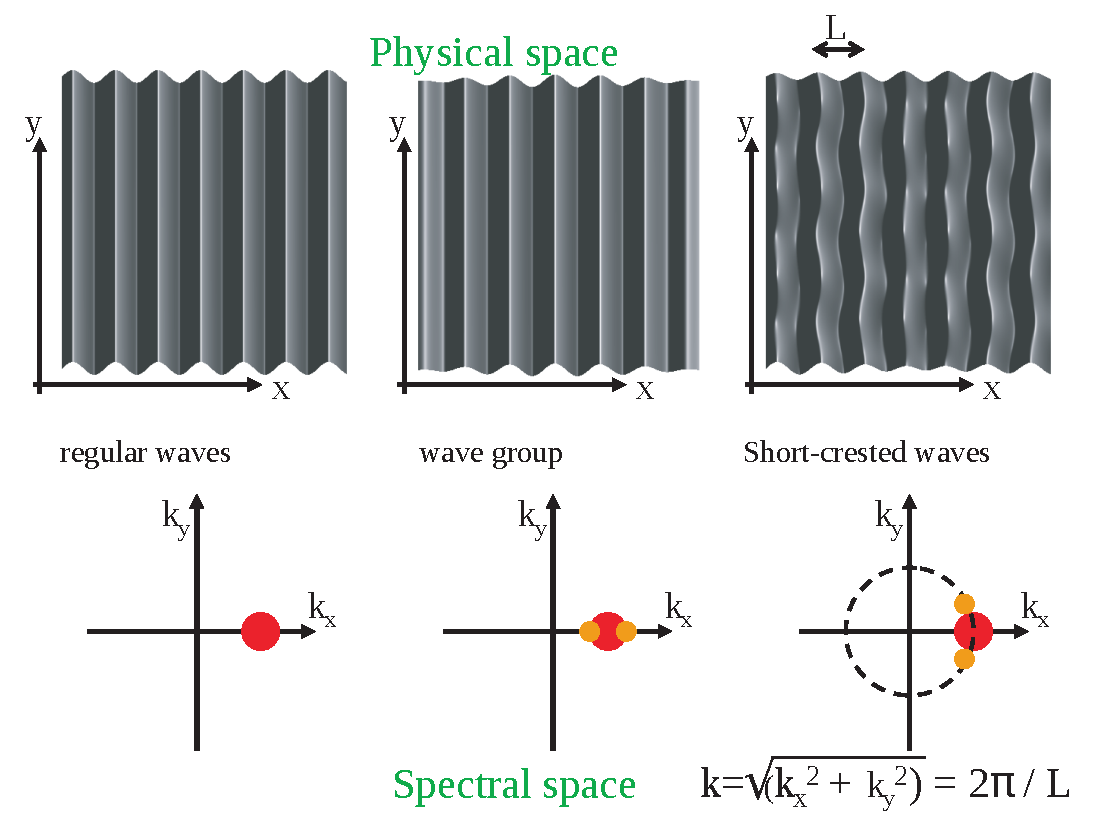
\includegraphics[width=0.8\textwidth]{FIGS_CH_MEASUREMENTS/spectres101_en.pdf}}
\caption{Relation between spectral and physical spaces. Schematic spectra of monochromatic waves (left panel) and modulated in terms 
of wavenumber or direction. For the last two cases, the surface is composed of three components.\label{fig:spectres101}}
\end{figure}
%%%%%%%%%%%%%%%%%%%%%%%%%%%%%%%%%%%%%%%%%%%%%%%%%%%%%%%%%%%%%%%%%%%%%%%%%%%%%
The reader is invited to try to recomposed a sea surface in the physical space from the spectrum produced by a numerical model,
\begin{equation}
\zeta(x,y,t)=\sum_{m}^{M}\sum_{n}^{N}\sqrt{2E(f_m,\theta_n)\Delta_f \Delta_\theta} \cos\left[ k_m \cos \theta_n x +k_m \sin \theta_n  y- \sigma_m + \Theta_0(m,n)\right],
\label{eq3.11}
\end{equation}
where $\Delta_f$ and $\Delta_\theta$ are the spectral resolutions, and $M$ and $N$ are the number of frequencies and directions used to discretize the spectrum.  
Rigorously, $M$ and $N$ should be taken infinite, but we may start with the typical resolution of  a 
spectral wave model, of the order of 30 frequencies and 24 directions, with a significant level of energy in maybe only 20 components. If you want to get a more realistic surface it is best to interpolate the spectrum on a fine spectral grid, before taking the inverse Fourier transform. 

The component amplitude $\sqrt{2E(f_m,\theta_n)\Delta_f \Delta_\theta}$  is consistent with the fact that the total variance 
elevation is the sum of the amplitudes squared divided by two, or the spectrum integral over the entire spectral domain. 
The phase $\Theta_0(m,n)$ can be taken randomly distributed over [0,2$\pi$]. The resulting surface will look smoother than 
an actual sea state, and the observed crest-trough asymmetry will not be reproduced. This is due to the random phase assumption 
that disregards the phases coupling between spectral components. You may add some nonlinear effects with the "choppy" method, shifting your elevation map using an estimate of horizontal displacement, giving more realistic wave crest shapes \citep{Nouguier&al.2009}.  %These issues are further addressed in \S\ref{random_harmonics}.

\section{Using spectra}
Skipping here the technical details necessary for a practical estimation of the spectrum  (see chapter \ref{ch_anaspec}), we now have a spectrum. Very nice, but what 
can we do with it? 

\subsection{Transfer function}\label{sub:transfer}
Depending on the application, one can transform the elevation variance spectrum. For a variable $A$ (for instance the bottom pressure), related to the  
surface elevation through a linear relation:
\begin{equation}
A=M\zeta,
\label{eq3.12}
\end{equation}
where $M$ is a complex number that takes values in the spectral space, the variance spectral density of $A$, $E_A$ is 
\begin{equation}
E_{A}(k_{x},k_{y})=|M|^{2}E(k_{x},k_{y})~\mathrm{or}~ E_{A}(f,\theta)=|M|^{2}E(f,\theta)
\label{eq:transfert}
\end{equation}
or any other equivalent expression in other spectral coordinates. For instance, the bottom velocity variance will be given from the polarization relation (\ref{polzeta})--(\ref{xi3}), that yield 
$M=\sigma \cos(\theta)/\sinh(kD)$, with $\theta$ the angle between the $x$-axis and the wave direction of propagation. We hence 
get the spectrum of the $x$-component of the bottom velocity.

Two of the most commonly used transfer functions are $M=\sigma$ for getting the surface orbital velocity magnitude in deep water, hence $M^2=4\pi^2 f^2$, and $M^2=\rho_w g/C_g=\rho_w g/(4 \pi f)$ for getting the energy flux in deep water. Using these transfer functions you get the surface orbital velocity variance 
\begin{equation}
<u^2+v^2>_{z=\overline{\zeta}}   =4\pi^2  \int_{0}^{\infty}  f^{2} E(f) {\mathrm d}f = 4\pi^2 m_2
\label{eq:moment_def}
\end{equation}
where $m_2$ is the second moment of the spectrum, and in general the  \textit{p-th} moment of the spectrum is defined as,
\begin{equation}
m_{p} = \int_{0}^{\infty}\int_{0}^{2\pi} f^{p} E(f,\theta)d\theta df
\label{eq:moment_def}
\end{equation}
Now, you may wonder why somebody would like to know the variance of the orbital velocity, well, it comes up, for example in Morison's equation that is the most widely used equation in offshore engineering to estimate forces on a structure \citep{Boccotti2000}, and other variances will matter for other applications. 

\subsection{Spectral and integral parameters: $H_s$, $T_p$ ...}\label{sub:param}
It can
be inconvenient  to describe a sea state by a two-variable function. Even when it is discretized into a numerical model,  typically 
over 30 frequencies and 24 directions meaning 720 spectral components, which is a lot of numbers to describe a sea state. This information can be 
summarized into a few meaningful parameters.

As the spectrum is a decomposition of sea surface variance, the most important parameter is certainly the variance $E$, often abusively called
energy. From the elevation variance $E$, we get a length scale  $\sqrt{E}$. Going back to sine waves, the variance is $a^2/2$ with $a$ the wave amplitude. Hence $\sqrt{2 E}$
is an equivalent amplitude  for random waves. More precisely, it is 
the root mean square amplitude. The root mean square wave height for a random wave is thus twice this amplitude
$H_{\mathrm{rms}}=2 \sqrt{2E}$.

For practical applications, the most widely used height scale is the \textit{significant wave height} $H_s$ that corresponds to the visual 
feeling given by the sea. From the wave height distribution we can define $H_{1/3}$ (see chapter \ref{ch1}). From the spectrum we define,
\begin{equation}
H_s \equiv H_{m0}\equiv 4 \sqrt{E} = 4 \sqrt{\int_{0}^{\infty} E(f) {\mathrm d}f}
\label{eq3.14}
\end{equation}
In practice $H_{m0} \simeq H_{1/3}$, this property can be demonstrated in the limit of a narrow spectrum \citep{Longuet-Higgins1952}. Following the recommendations of 
the World Meteorological Organization, 
we shall consider $H_{m0}$ to be \emph{the} definition of the significant wave height $H_s$. The "$m0$" index indicates that it is based on the zeroth moment of the spectrum. 


In many cases, the directional information is not available, and we only have the frequency spectrum $E(f)$. 
This distribution of the energy as a function of frequency contains information on the typical time scales of the signal. $E(f)$ generally exhibits 
a sharp maximum around the frequency $f_p$, $E(f_{p})=E_{\max}$. $f_p$ is the peak frequency, corresponding to the peak period $T_{p}=1/f_p$.  
This peak period can be noisy in the presence of several peaks, as in Fig. \ref{fig:Hawaii_spectrum}.
The frequency distribution can also be characterized from the spectral moments, $m_p$, 
\begin{equation}
T_{m0,p} =  \left[m_p/m_0\right]^{-1/p} \simeq \left[\left(\int_{0}^{f_{\max}} f^{p} E(f) df\right)/\left({\int_{0}^{f_{\max}} E(f) {\mathrm d}f}\right)\right]^{-1/p}.
\label{eq3.17}
\end{equation}
The most widely used periods are $T_{m0,-1}$, $T_{m0,1}$, $T_{m0,2}$. Each of these has a more or less weight on low frequency part of the spectrum.
If one is interested in an effect proportional to $f^2$, as is  the case of the wave forces exerted on a structure, it is reasonable to use $T_{m0,2}$.
Besides, $T_{m0,2}$ is very close to the mean period $T_z$ given by  wave-by-wave analysis. Note however that in practical calculations, $T_{m0,2}$ depends on the choice
of $f_{\max}$. The values of the different periods for a typical spectrum are shown in figure 
\ref{fig:Hawaii_spectrum}.
%%%%%%%%%%%%%%%%%%%%%%%%%%%%%%%%%%%%%%%%%%%%%%%%%%%%%%%%%%%%%%%%%%%%%%%%%%%%%%%%%%%%%
\begin{figure}[htb]
\centerline{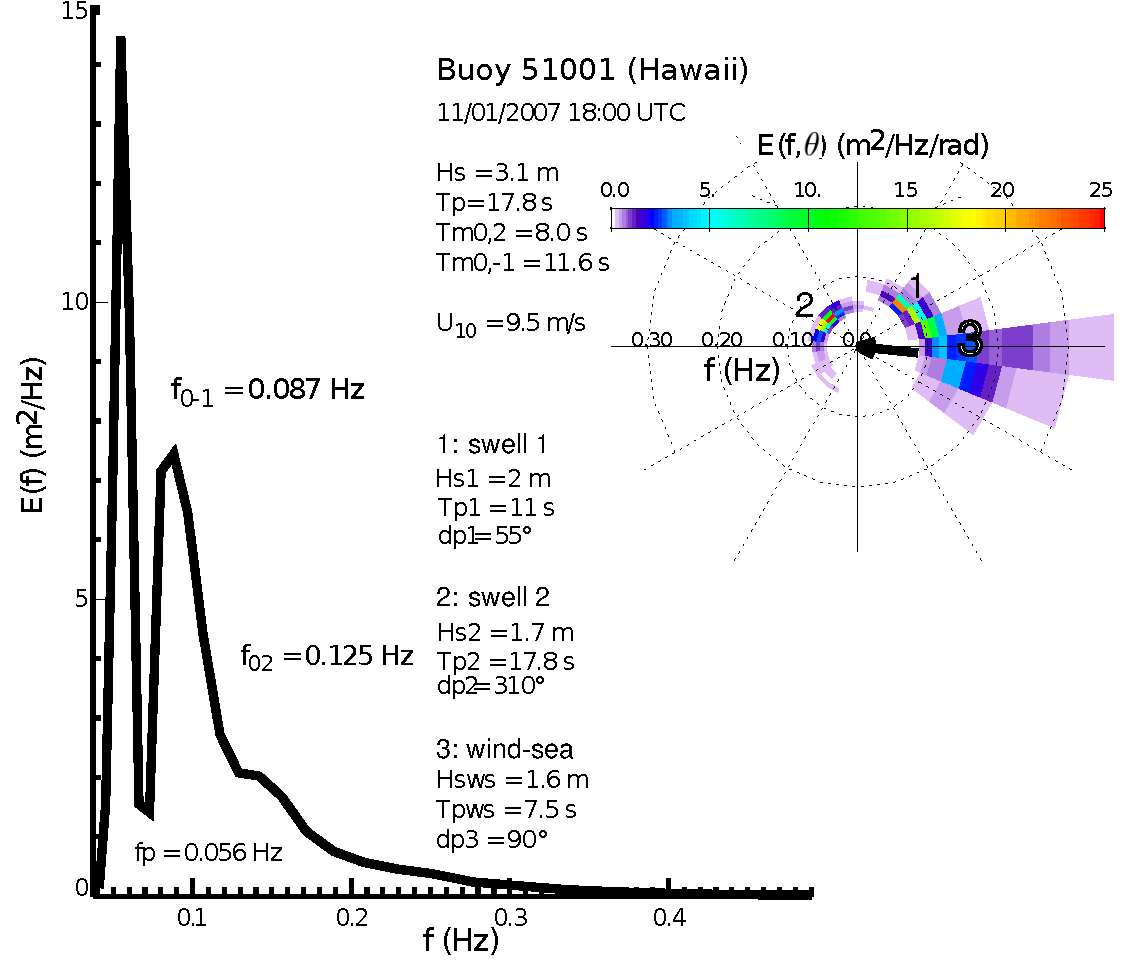
\includegraphics[width=0.7\textwidth]{FIGS_CH_MEASUREMENTS/exemple_spectre_Hawaii.pdf}}
\caption{
Typical example of a oceanic spectra in tropical area, measured by buoy 51001, moored 350 km North West of Kauai island, on January 11, 2007. 
The different peak and mean periods are indicated along with the parameters produced by a decomposition of the spectrum into a primary
swell, secondary swell and wind sea. This analysis is generally not possible without directional information. Note that the wind sea only appears 
as a soft "shoulder" to the right of the secondary swell, while it comes from a different direction. This shows the possible difficulty of 
separating swell and wind sea from a frequency spectrum. Also note that the significant 
wave height $H_s$ is less than the sum of $H_{s1}$, $H_{s2}$, $H_{sws}$, of the three systems: the energy can be summed but the wave heights cannot.
Namely $H_s=\sqrt{H_{s1}^2+H_{s2}^2+H_{sws}^2}$.}
\label{fig:Hawaii_spectrum}
\end{figure}
%%%%%%%%%%%%%%%%%%%%%%%%%%%%%%%%%%%%%%%%%%%%%%%%%%%%%%%%%%%%%%%%%%%%%%%%%%%%%%%%%%%%%%%%%%%


Finally, we define, 
\begin{eqnarray}
a_{1}(f) & = &\int_{0}^{2\pi} \cos{\theta} E(f,\theta)d\theta /\int_{0}^{2\pi} E(f,\theta)d\theta, \label{a1def} \\
b_{1}(f) & = & \int_{0}^{2\pi} \sin{\theta} E(f,\theta)d\theta /\int_{0}^{2\pi} E(f,\theta)d\theta ,\label{b1def} \\
\end{eqnarray}
that can be estimated from the elevation spectrum $E(f)$ and the elevation-horizontal displacements
co-spectra, $E_{xz}$ and  $E_{yz}$, as detailed in chapter \ref{ch_anaspec},   eqs. (\ref{Exz})--(\ref{Eyz}). 

The mean wave direction at frequency $f$ is, 
\begin{equation}
\theta_{m}(f)=\arctan(a_{1}(f)/b_{1}(f)),
\label{eq3.20}
\end{equation}
and the directional spreading, as defined by \cite{Kuik&al.1988} is the standard deviation (in radians) of the spectral width
in the limit of a narrow spectrum,
\begin{equation}
\sigma_{\theta}(f)=\left[2(1-(a_{1}^{2}(f)+b_{1}^{2}(f))^{1/2}) \right]^{1/2}.
\label{eq3.21}
\end{equation}
For equal energies in opposite directions, $\sigma_{\theta}$ is maximum at 
$\sqrt{2}$ radians, which is $81\,^{\circ}$. 

The directional wave properties of the dominant waves, can also be characterized with the 
mean direction and directional spreading of the spectral peak: $\theta_{m}(f_{p})$ and $\sigma_{\theta}(f_{p})$. 
$\theta_{m}(f_{p})$ is often referred to as "main direction", while the mean direction would rather be an average
over the entire spectrum,
\begin{equation}
\theta_{M}(f)=\arctan \left(\int_{0}^{\infty} b_{1}(f) E(f)df/\int_{0}^{\infty} a_{1}(f) E(f)df\right)
\label{eq3.22}
\end{equation}
With all these directions, one must be careful with the directional convention. The directions are usually counted
from North (direction 0), progressing clockwise (90 east, 180 south, 270 West). However, depending on the authors, the direction convention is either meteorological (direction
from where the waves or wind are coming, this is the convention used in the present manuscript) or oceanographic convention
(direction toward which the waves or currents are moving). Be careful!

 

 \section{Random waves \textit{in situ} observations}
 The most common usage of wave time series is the determination of the frequency spectrum $E(f)$ and, when more than 
 one variable are measured, the directional wave spectrum $E(f,\theta)$ may be estimated. Details of this processing 
 given in chapter \ref{ch_anaspec}. In practice, the most common in situ 
 instruments for wave measurements are surface-following buoys or bottom-mounted pressure gauges or ADCPs.  
 
 \subsection{Wave gauges}
 These are reference sensors that directly measures the free surface elevation $\zeta(x,y,t)$ at a fixed horizontal position $(x,y)$. 
 The measure is done through the 
electrical resistance or capacity of one (or two) conducting wires forming a loop closed by the sea surface. This type of sensor is widely 
used in the laboratory, but it is not so common at sea because this requires a fixed  platform
 and the wires are susceptible to damage by small floating debris. Also, the large wave heights encountered in the field require long 
 enough gauges. These wave 
gauges can also be mounted on a buoy that filters out the long waves through its motion \citep{Graber&al.2000}. Wave gauges are most often 
associated in an array (see below) of several gauges synchronized and mounted on a single platform so as to 
provide a wave direction estimation \citep{Cavaleri&al.1981}.

The direct measurement of surface elevation can also be performed by radar and LIDAR systems, which determine the  
distance to the sea surface from the travel time of an electromagnetic or sound wave, and that can likewise be arranged in an fixed array or integrated 
in a scanning system.


  \subsection{Wave buoys}
    Buoys measure either the successive positions and velocities, determined by a global navigation satellite system (such as the Global Positioning System - GPS) or 
    vertical acceleration recorded by a buoy floating at the free surface that give after a double integration in time, 
  a surface elevation signal $\zeta(x,y,t)$. Depending on the type of instrument and on the presence of currents, the horizontal position $(x,y)$ is not fixed but 
  nearly follows the wave orbital 
motion. This later property may be annoying for purists of the wave profile, as it partly filters out the free surface nonlinearity (the linear 
Lagrangian motion involves a part of the nonlinear Eulerian motion). In addition to the heave measurement, that was for long the most common, the wave 
direction can be determined by measuring the horizontal accelerations that yields, through double integration, the horizontal displacement $x$ 
and $y$ (figure \ref{Datawell_xyz}). 
\begin{figure}
\centerline{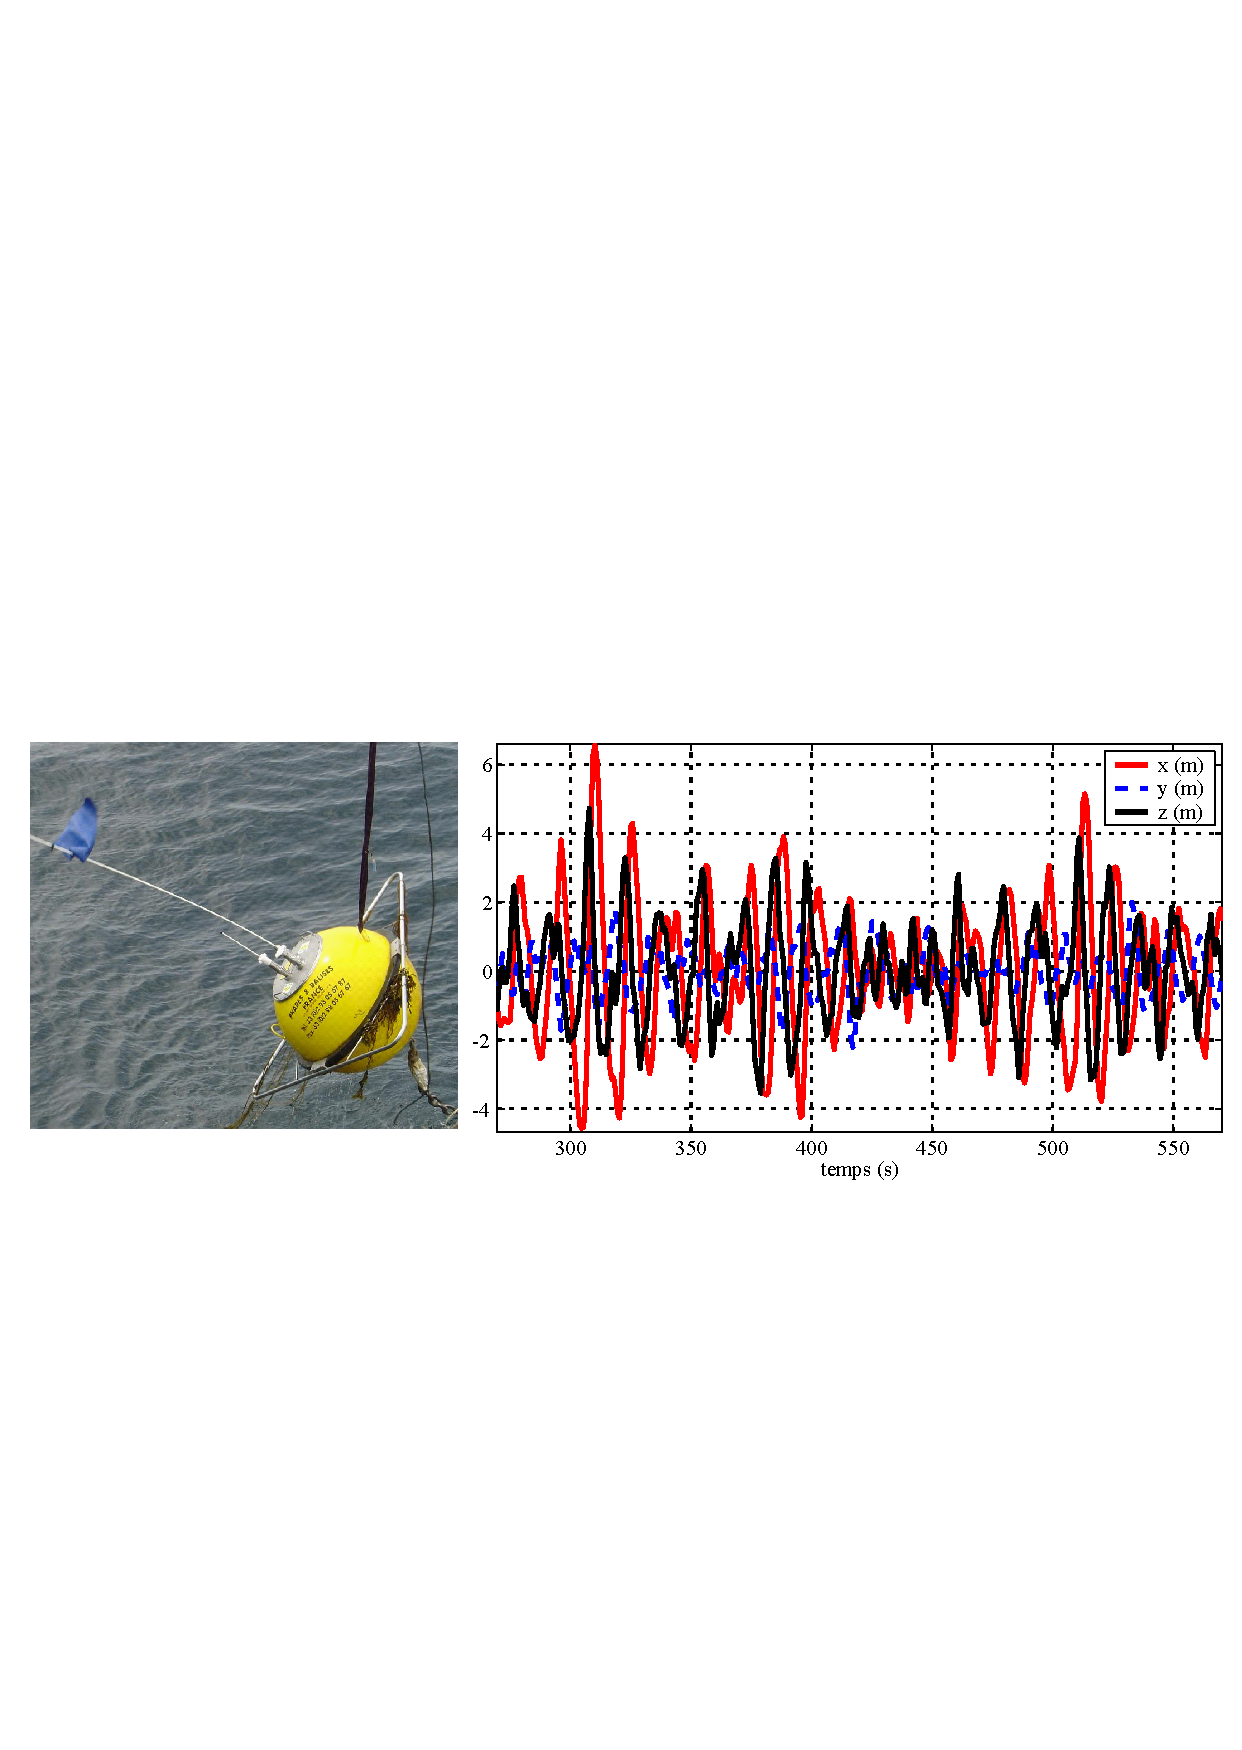
\includegraphics[width=\textwidth]{FIGS_CH_MEASUREMENTS/Exemple_DWIROISE2004all_plus.pdf}}
\label{Datawell_xyz}
\caption{Left panel: Deployment of a  Datawel Waverider buoy, 0.9 m of diameter, equipped with a (long) HF radio antenna and 
with a (short) Orbcomm satellite antenna for data transfer. Right panel: examples of displacements measured by this buoy offshore Crozon in May 2004. 
(same time series as in figure \ref{FigWaveriderTSz}). Of course, the 10~m high waves were not measured by the times of the buoy deployment.}
\end{figure}
 The use of  precise satellite positioning now allows a direct measure of the 3-component position and velocity, the latter being generally more accurate \citep{Herbers&al.2012}. Many companies have commercialized such buoys.

The largest buoys generally use a measurement of the components $\partial \zeta /\partial x$ and $\partial \zeta/ \partial y$ and of the local free 
surface slope: pitch and roll as the first prototypes of \cite{Longuet-Higgins&al.1963} and \cite{Cartwright&Smith1964}. This is the case of the US 
National Data Buoy Center (NDBC) 3-m diameter buoys.
Details of buoy processing are given in chapter \ref{ch_anaspec}. Both methods, acceleration and pitch-roll allow, thanks to the three signal covariance, 
the determination of the first four Fourier coefficients 
of the angular distribution, also known as angular moments,
\begin{itemize}
  \item  $a_1$ and $b_1$, defined by (\ref{a1def})--(\ref{b1def}) and calculated from the co-spectra $E_{xz}$ and $E_{yz}$ (equations \ref{Exz}--\ref{Eyz})
\item $a_2$ and $b_2$, defined as $a_1$ andf $b_1$ but with $\cos \theta$ and $\sin \theta$ replaced by $\cos 2 \theta$ and $\sin 2 \theta$, respectively.
\end{itemize}

A more complete measure of the directional spectra from floating buoys has been developed but has not been as successful as expected: the cloverleaf buoy that consists in three 
pitch-roll buoy linked to each other \citep{Mitsuyasu&al.1975}. In principle this layout provides a measure of the surface curvature and the Fourier coefficient up to $a_8$ and $b_8$.
From a conventional buoy, one has to infer the function $S(f,\theta)$ from only the four independent number $a_1$, $b_1$, $a_2$ and $b_2$. This is not so much a 
measurement problem, but rather one of choosing a statistical estimator. There are many method for this. Among these, the Maximum Entropy Method \citep[MEM][]{Lygre&Krogstad1986}, 
has the advantage of conserving the angular moment  $a_1$, $b_1$, $a_2$ and $b_2$. The MEM method tends however to 
to give a bimodal shape (two-peak spectra), which is often \citep{Ewans1998} but not always realistic \citep{Benoit&al.1997}.

Other recent analysis techniques aim at increasing the the directional resolution of this kind of measurements. For instance, \cite{Donelan&al.1996}, 
have proposed an interesting method based on a wavelet transform. Unfortunately their method assumes that for any given frequency 
the wave field is dominated by waves coming for one single direction, which is not the case. This analysis yields a very high directional resolution, and can be interesting 
to detect the presence of waves from a given direction, but it cannot be interpreted as a directional spectrum as it leads to a low bias in the directional spreading. Other methods can be biased and 
should be avoided. This is 
the case of the maximum likelihood method (MLM) which yields output spectra that are systematically too broad and have moments $a_1$, $b_1$, $a_2$ and $b_2$ that 
are different from the input parameters.
 
 \subsection{Pressure gauges}
 When surface elevation measurements are too expensive or not possible, which may be due to strong currents incompatible with mooring lines, breaking waves in the surf zone, a usually good alternative is the measurement from bottom-mounted sensors. The most common and robust are pressure gauges that can be used to measure 
 tidal elevations at the same time. To recover the surface elevation from the pressure signal, we can invert the linear transfer function given by eq. (\ref{pression}), 
 namely, for a sensor at a height $h_d$ over the bottom,  $M=\rho_w g \cosh(kh_d)/\cosh(kD)$, with $k$ estimate from the frequency $f$ of each spectral component of the time series, using the Airy wave dispersion relation. In shallow water and for waves of large amplitudes, this method often underestimates the wave height because the linear dispersion is not very accurate \citep{Filipot&al.2010,Bonneton&Lannes2017}. The water depth $D$ is also given by the measurement of 
 the mean pressure once it is corrected for the atmospheric pressure. Because the elevation to pressure transfer function $M$ decreases when  $k$ increases, it is usually impossible to recover  wave elevations for frequencies above a cut-off value $f_c$. That value $f_c$ is a function of water
 depth, instrument noise, background noise (usually due to currents), but also of the directional wave spectrum. Indeed, figure \ref{fig:pressure_with_2ndorder}
 shows an example of data recorded in 100~m depth, in which the second order pressure is larger than the linear pressure for frequencies above 0.13~Hz. As discussed in part 3, 
 this second order spectrum is a function of the frequency spectrum $E(f)$ but also of the directional wave distribution. In that case, it is not possible 
 to recover $E(f)$ for frequencies above 0.12~Hz. For example, on day 4, the yellow-orange sloping line at frequencies 0.05 to 0.1 Hz is 
 a due to swell waves arriving from a distance of about 4000~km (see explanations in chapter \ref{ch3}, eq. (\ref{prev lin1})). 
 At the same time, there is a fainter blueish line at twice these frequencies which is caused by the 
 second order effect. The vertical blue stripes above 0.13~Hz are caused by the tidal current effects on the directional wave spectrum \citep{Ardhuin&al.2013}.
 %%%%%%%%%%%%% figure
\begin{figure}[htb]
\centerline{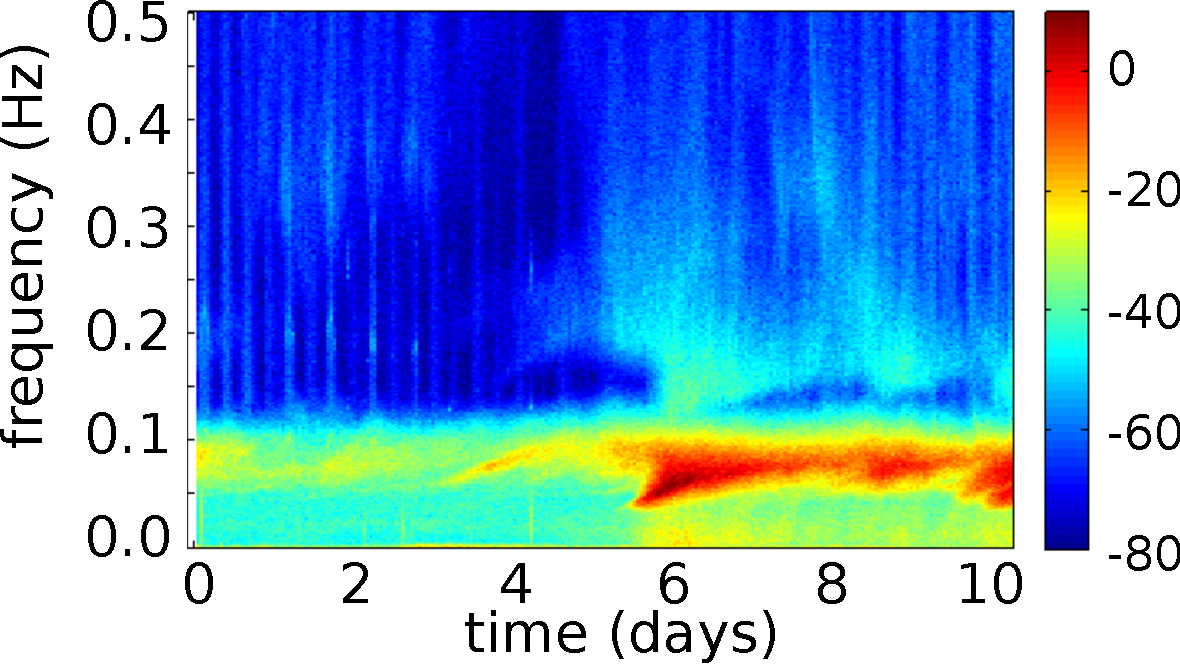
\includegraphics[width=0.7\textwidth]{FIGS_CH_MEASUREMENTS/pressure_with_2ndorder.pdf}}
%\vspace{3.64in}
  \caption{Bottom pressure spectra}
    {Time-frequency diagram of the pressure recorded over 11 days in 100~m depth off the French Atlantic coast in October 2015.  The colors show the pressure level in dB relative 
    to 1~m$^2$/Hz times $\rho_w^2 g^2$. These measurements were performed by a very sensitive Paroscientific piezo-electric sensor, included in a RBR-duo 
    system, with a noise level below -80 dB. At our depth of 100~m, the usual linear pressure signal, with a level between -40 to 10 dB, can be used to recover 
    the surface elevation spectrum for frequencies below 0.12~Hz. At higher frequencies, the pressure is dominated by a second order effect due 
    to waves in opposite directions \citep[e.g.][]{Miche1944b,Ardhuin&al.2013}. That effect has very important consequences for seismology, as discussed in part 3.} \label{fig:pressure_with_2ndorder}
\end{figure}
%%%%%%%%%%%%% end of figure

 
\subsection{P-U-V sensors}
As indicated by its name, this sensor measures the pressure $p$ and the two horizontal components of the velocity, $u$ and $v$. It is indeed the 
combination of two instruments: a current meter (acoustic, electromagnetic because a high sampling rate is required) and a pressure sensor, often 
piezo-electric. This instrument is of particular interest as it is designed to be installed on the sea bottom. It is the simplest mooring you may imagine, if one 
is not too worried about fishermen, for instance. Of course, it is difficult ut not impossible to recover real time data (cables, acoustical modems with surface buoys...).

We have seen in Chapter 2 that the fluid pressure and velocities exponentially decay from the surface to the bottom with a typical scale which correspond 
to the wave length 2$\pi/k$. The "P-U-V" sensor is thus perfect if one wish to measure the agitation at the bottom. To measure the wave heights one may use
the theory that provide transfer functions between pressure, velocities, elevation, etc (equation \ref{eq:transfert}). In this situation, the closer to 
the surface, the more reliable will be the measurement (e.g. an instrument mounted on a floating of fixed platform).

 \subsection{Sensor arrays and ADCPs}
A set of wave gauge can be combined to record more covariances between the measurements. This kind of 
measure allowed to get the first accurate spectra \citep{Donelan&al.1985} and is particularly used for the air-sea interaction studies, 
for which the short waves spectrum is crucial \citep{Graber&al.2000, Pettersson&al.2003}. It is essential to synchronize the sensors with 
an accuracy that is small compared to the measured wave period. Similar techniques are employed in RADAR and SONAR technologies to determine the sources of echoes. The original array processing algorithms 
used for waves were actually developed for seismology.

 These techniques have been largely applied to pressure sensors arrays with a number of statistical methods for the spectrum estimation 
 \citep[e.g.][]{Davis&Regier1977, Long&Hasselmann1979, Pawka1983, Herbers&Guza1990}. An example of a spectrum is given in Figure \ref{wave spectra} 
determined from a coherent array of pressure sensors deployed in 8m depth on the site of the US Army Corps Field Research at Duck, North Carolina. 
For large arrays, the underwater instruments positioning much be very accurate. An acoustical positioning is generally used.
%%%%%%%%%%%%% figure
\begin{figure}
\centerline{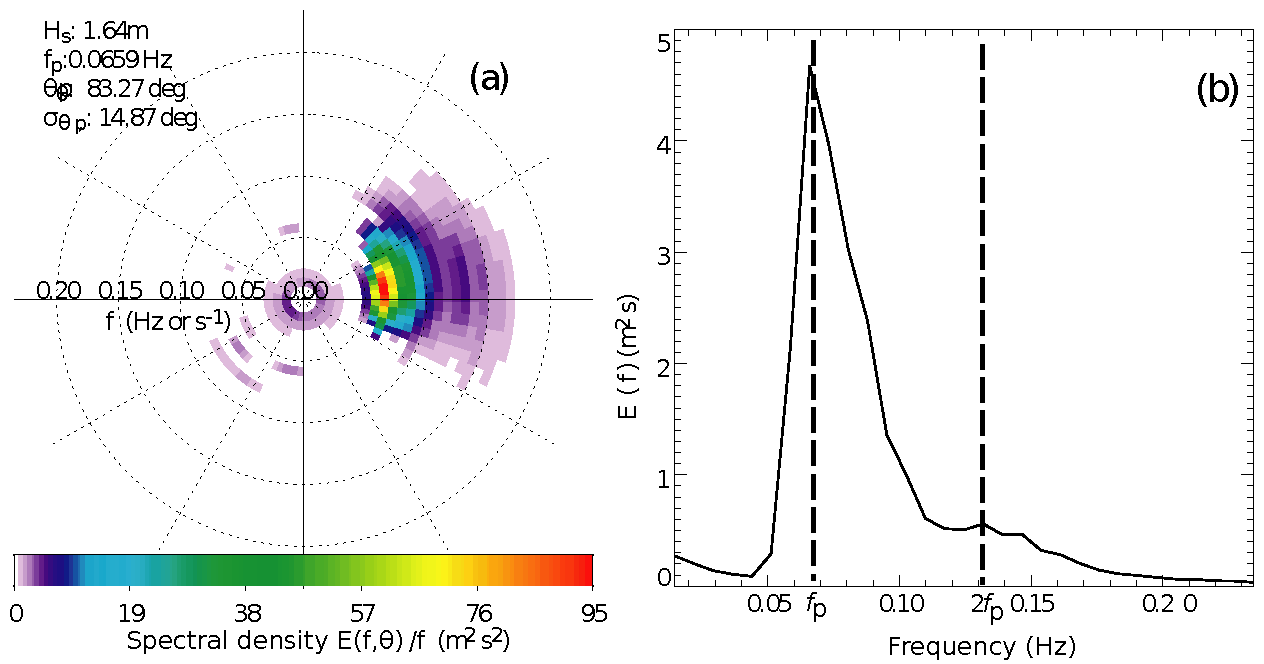
\includegraphics[width=0.6758\textwidth]{FIGS_CH_MEASUREMENTS/introduction_fig1.pdf}}
\caption{(a) Example of frequency-direction wave spectra, divided by frequency, computed from 8m depth pressure measurements in Duck, NC, October 
19, 1994, 7:00 (EST). (b) Corresponding Frequency spectra whose secondary peak matches the first harmonic of the spectral peak 
($f=2f_p$), and which is likely due to the effect of nonlinear interactions that are of great importance in shallow water.}
\label{wave spectra}
\end{figure}
%%%%%%%%%%%%% end of figure
  The directional resolving power of the array generally increases with the number of sensors in the array \citep[see][]{Kinsman1965}. 
  Arrays of pressure sensors are excellent reference instruments for measuring the spectra of dominant waves,  but they 
are relatively expensive to deploy and maintain. \cite{OReilly&al.1996} used such an array for the validation of directional properties of two different types of 
buoys. %However, comparisons have shown that for the parameters estimated from the the moments  $a_1$, $b_1$, $a_2$ and $b_2$, 
%the Datawell wave buoy, for instance, gives excellent results \citep{OReilly&al.1996}. Sensors arrays get useful only when further details on the 
%wave spectra are required (separation of incident and reflected waves, or of different wave systems, etc...). 

A recent and convenient alternative is the use of current profilers (ADCP).  The combination of the velocities measured by different acoustic beams, 
allows, in principle, for an interesting measure of the directional spectra. However, the typical noise of up-looking ADCPs does not allow a 
higher angular resolution than that of a simple P-U-V \citep{Herbers&Lentz2010}. The main benefit of ADCPs, however, is the use of measurements close to the sea surface, 
where the wave motion is less attenuated than at the bottom. 

\section{Optical measurements}
Waves are usually the first thing that you see when looking at the sea. But turning beautiful pictures into numbers for scientific analysis is 
not so easy. We will not discuss here the techniques that are mostly used in the laboratory (e.g. light refraction across the air-sea interface), but 
instead we present the main methods in use for application to real ocean waves. 
\subsection{From stereo-photography to stereo-video}
The first methods used to measure wave shapes were based on stereo-photography: pairs of photographs taken at the exact same time can be analyzed to 
produce a 3D map of the sea surface \citep{Schumacher1939}. The basic principle is to determine the $(x,y,z=\zeta(x,y))$ coordinates of points that have been 
identified in both images. This identification can be done using automatic correlation analysis. The pair of pictures can be obtained from a single platform to cover a modest area and reveal interesting 
details about the wave shapes \citep{Banner&al.1989}, typically less than 30 by 30~m, 
or from a pair of aircraft to get a view of a much broader region \citep{Cote&al.1960,Holthuijsen1983b} and produce a full directional 
wave spectrum. 
%%%%%%%%%%%%%%%%%%%%%%%%%%%%%%%%%%%%%%%%%%%%%%%%%%%%%%%%%%%%%%%%%%%%%
\begin{figure}[htb]
  \center{\noindent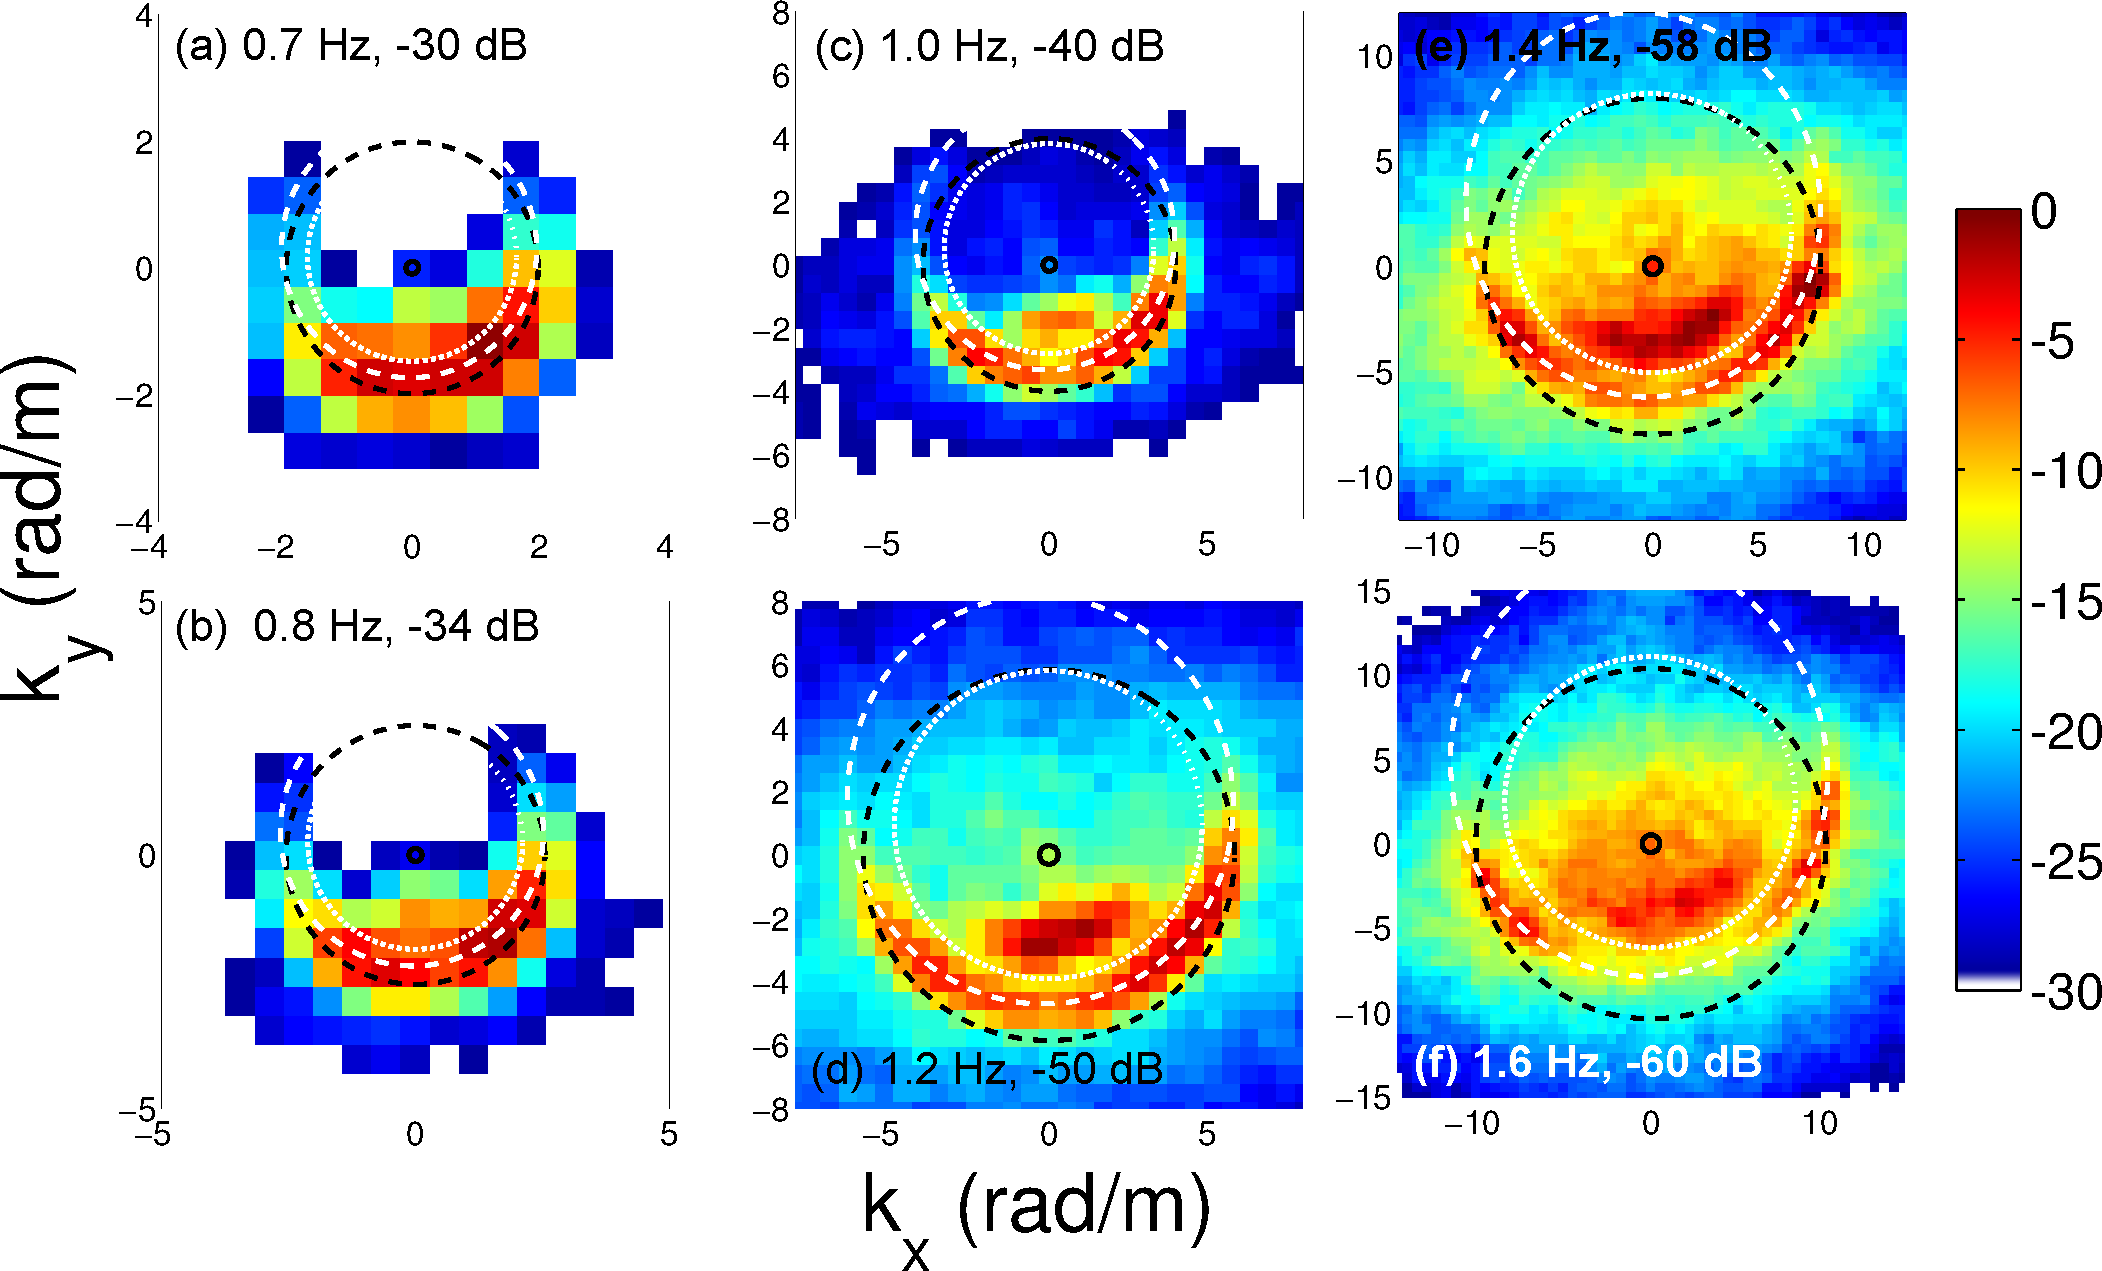
\includegraphics[width=0.8\linewidth,angle=0]{FIGS_CH_MEASUREMENTS/kxky_spec1_nosmooth.pdf}}\\
  \caption{Slices of the double-sided spectrum for positive apparent frequencies 0.7, 0.8, 1.0, 1.2, 1.4 and 1.6 Hz. The energy appears in the direction from 
           where it is coming. For each panel the color scale spans 30 dB with the dark red corresponding to the power indicated on 
the figure (e.g. -30 dB) relative to 1~m$^4$/Hz. Note that 1.4 and 1.6 Hz are twice 0.7 and 0.8 Hz, so that the first harmonic of the components in (a) and (b) 
           appear at approximately twice the wavenumbers in panels (e) and (f). In each panel, the linear dispersion relation without current is plotted in black, and the  white dashed line gives the linear dispersion with a uniform current $U= 0.15$ m/s oriented towards the trigonometric angle 99 degrees. The white dotted  line marks approximately the separation between 
the linear part of the spectrum and the faster non-linear components (Adapted from Leckler et al. 2015). } \label{fig:kxky}
\end{figure}
%%%%%%%%%%%%%%%%%%%%%%%%%%%%%%%%%%%%%%%%%%%%%%%%%%%%%%%%%%%%%%%%%%%%%
Now that everyone is carrying a digital camera around, and that stereo processing is much more common, there are many opportunities 
to measure the full evolution  of the sea surface in space and time $\zeta(x,y,t)$. Recent efforts by \cite{Benetazzo2006} and \cite{Gallego&al.2011} 
have demonstrated the capabilities of stereo processing, leading to new applications \citep{Fedele&al.2013,Leckler&al.2015}. Latest developments include  
auto-calibration and the proper motion corrections needed for ship deployments. A general issue that remains is that not all light conditions are favorable. Alternatively, the use of 
more expensive infrared cameras or polarization cameras is a very interesting extension for overcoming the variability of lighting conditions and 
the lack of texture at small scale 
for a correlation analysis \citep{Sutherland&Melville2013,Laxague&al.2015}.

The great advantage of having the full surface $\zeta(x,y,t)$, is that we can now measure a 3D spectrum, without the need to use linear wave theory. 
This is most important for the short wave components, for which nonlinear contributions are important. Figure \ref{fig:kxky} shows slices of the 3D spectrum 
at a constant frequency. These are obtained from a stereo-video system installed 11~m above the water in a platform in the Black Sea. The image processing 
uses the epipolar method: the position of the sea surface is obtained only by a knowledge of the geometry of the camera system.
This record from October 4, 2011, was acquired when the wind speed was 14~/s and the wave  peak frequency is $f_p=0.33$~Hz \citep{Leckler&al.2015}. The 
Non-linear contributions to the frequency spectrum dominate for $f > 4 f_p$. For example at $f=1.2$~Hz, there is more energy in the peak located near $(k_x=0,k_y=-3)$ 
than along the linear dispersion relation shown wit the white dashed line. 
Such non-linear effects are also important for the statistics of extreme wave heights, as shown by \cite{Fedele&al.2013} and \cite{Benetazzo&al.2017}.



\subsection{Using polarization and/or light intensity}
Such a stereo system has difficulties in measuring waves with frequencies higher than 1.4~Hz that have small heights. Other measurement techniques that 
are directly sensitive to slopes are better suited for these shorter components: these include polarimetry \citep{Zappa&al.2008} or a measurement of 
the radiance that can also be combined with the epipolar method \citep{Gallego&al.2011,Yurovskaya&al.2013}. 

Such a technique can also be applied to high resolution airborne or satellite imagery (with pixel sizes less than 30~m in order to resolve waves). 
\cite{Kudryavtsev&al.2017} have particularly taken advantage of the O(1~s) time lag in the acquisition of the different color channels of the Multi Spectral Instrument 
on board Sentinel-2. Clouds or haze obviously limit the application of optical methods, which is why radar is often preferred for wave remote sensing. 



\subsection{Surface wave radar}
An extreme case of grazing angle occurs when the radar waves propagate along the surface. This kind of propagation is possible
in the HF-VHF range (from 2 to 50 MHz). This surface wave allows indeed to get information beyond the horizon. 

%%%%%%%%%%%%% figure
\begin{figure}[htb]
\centerline{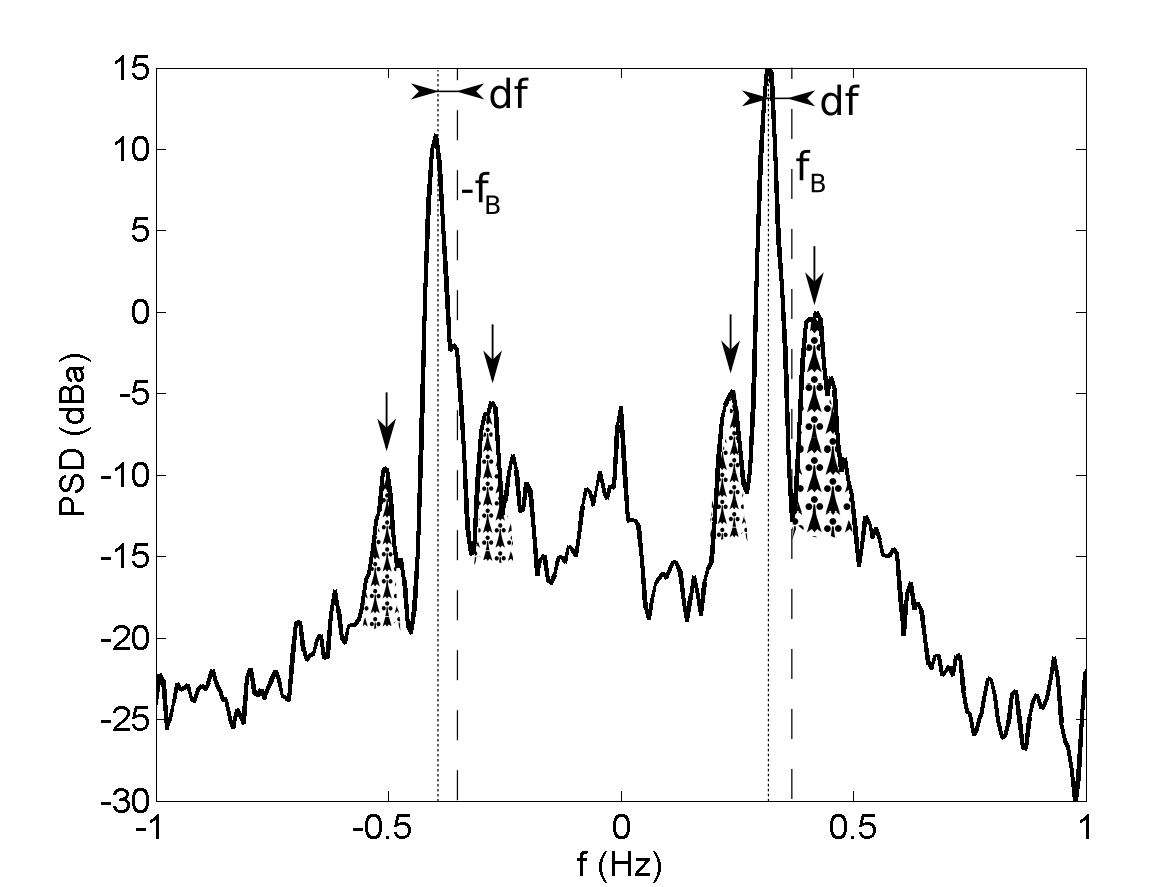
\includegraphics[width=0.5\textwidth]{FIGS_CH_MEASUREMENTS/Spectre_bin_10_touch.png}}
%\vspace{3.64in}
  \caption{Example of Doppler spectrum from a HF radar.}{This measured spectrum comes from the Porspoder radar (Finistere, France). 
The radar frequency is 12.4~MHz, corresponding to a wavelength $L_e=2 \pi/k_e=24$~m. The main echoes is due to Bragg scattering, 
which selects the ocean waves with a wavelength $L_e/2=12$~m that propagate towards ($f > 0$)  or away from the radar ($f<0$). 
Multiple scattering by waves with wavenumbers  $\kb_1$ and $\kb_2$, such that $2 \kb_e = \kb_1 + \kb_2$
gives the 'second order echoes'. At first order, i.e. for linear waves, the waves of wavenumber $k_w=2 k_e$ 
have a frequency $f_B=\pm \sqrt{g 2 k_e} =\pm 0.36$~Hz  in deep water. The anomaly $df$ of the two highest peaks in the Doppler spectrum 
indicate that the phase speed $2 \pi f / k$ is different from the linear wave theory without current. 
the main reason for that difference is usually the presence of a current, with a velocity $U_r=2 \pi df / (2 k_e)$ in the direction of the radar. }\label{HFspectrum}
\end{figure}
%%%%%%%%%%%%% end of figure

The radar reflection is well explained by Bragg theory, with the maximum backscatter power at the Doppler frequency $f_D$ occuring for 
electromagnetic incident and reflected wave numbers vectors $\kb_i$ and $\kb_r$ that match with the wavenumber $\kb_w = \pm \kb_i \mp \kb_r$ 
and and the wave frequency $f_D=f$, where $f$ and $\kb_w$ are related by the linear dispersion relation. 
In the monostatic configuration where the receiving and transmitting antenna are almost at the same place, we have $\kb_i = \kb_e$,  $\kb_r= - \kb_e$, 
and $\kb_w = 2 \kb_2$. 

The observed Doppler spectrum can be
interpreted as the superposition of simple reflections (or first order reflections) and multiple reflections. 
The extraction of sea state spectra is possible from the second order that is a convolution of the spectrum 
\citep[see for instance][]{Wyatt2000}. These second order echoes are weaker than first order echoes at Bragg frequencies. The main echoes are used for currents measurement. Their frequency provides a measurement of the Bragg wave phase velocity. The deviation 
of this phase velocity from the expected linear wave phase speed can be interpreted as a surface drift current \citep{Ardhuin&al.2009b}. 
This current includes non-linear corrections to the phase velocity, which is like a filtered Stokes drift \citep{Stewart&Joy1974,Broche&al.1983,Ardhuin&al.2009}.
The secondary peaks are caused by either the multiple reflection of radar waves, or the single reflection off nonlinear wave components. 
In some cases a peak can be seen at the frequency $\sqrt{2}f_B$ which corresponds to the reflection from the first harmonic of waves with wavenumber 
$\kb = \pm \kb_e$, which have a frequency, $2\sqrt{g k_e}$ in deep water. Because different wave components have different sensitivities to the current profile, 
it is possible to use that peak to measure the vertical shear of the current \citep{Ivonin&al.2004}. 


%\section{The limitations to the usual wave spectrum}
%The spectrum gives the full statistical properties of waves, provided the components are effectively independent. Yet, this is not exactly true as waves are slightly nonlinear. Two main relations exist between components: the presence of harmonics and modulations. The first effects comes from the fact that a single nonlinear wave train corresponds to several spectral components whose wave number and frequency are multiple of that of the carrier wave. Rigorously speaking, one needs the 3D spectrum $E(f, \mathbf{k})$ to discern these harmonic waves that do not follow the linear dispersion  (Figure \ref{fig:kxky}). The 3D spectrum estimation requires specific instruments, mapping the surface in space and time. The link between the  3D spectrum and the linear part of the spectrum is the topic of ongoing research. The calculation technique of dressed and undressed spectrum presented by  \cite{Elfouhaily&al.2003}  is a possible approach: the undressed spectrum corresponds to the linear part and the dressed part to the nonlinear spectral contents. To lowest order, however, the full spectrum  can be obtained by the second order correction \citep{Janssen2009,Leckler&al.2015}. 

%The modulation effect is a bit more complex. Typically, short waves in the presence of much longer waves see their environment modified. In particular, the apparent gravity felt by short waves is the standard gravity plus the vertical acceleration induced by the longer waves motion. In the same fashion, the long waves orbital velocities acts as a variable current on the short waves.  These effects are one of the likely causes of the higher breaking rate of short  waves at the crest of long waves \citep{Dulov&al.2002,Guimaraes2018}. The short wave spectra is hence modulated by the long waves. In practice, for the wind sea, such effects are weak for waves with frequency less that three times the peak frequency \citep{Banner&al.1989}. This factor 3 on the frequency corresponds to a factor 10 on the wavelength (in deep water).

%Modulations can be caused by other effects than the presence of other waves. In particular, if the medium in which the wave propagate is not homogeneous, then the wave field will contain wavelengths that are interferences between the medium and the waves, and that do not correspond to the linear dispersion relation.  These non-homogeneities can be variations in water depth, current, gravity, surface tension ... 

%If these modulations occur  at scales similar to the wavelength, besides the local effect on the waves there is also a scattering of the waves with the generation of waves in other directions, frequencies, or other types of waves, such as the Bragg scattering  caused by underwater topography that is described in chapter \ref{ch5}, or the generation of seismic waves over a sloping bottom in  chapter \ref{chsismo}. These scattering effects result in an evolution of the spectrum in space and time. 

%If the scales are shorter than the wavelength, then the medium is a 'meta-meterial', which 
%can exhibit funny properties like negative refraction indices and can be used to create 'invisibility shields'. Although 
%these effects can be created in the laboratory, they may not be relevant for ocean waves, due to 
%the random nature of waves and the generally irregular patters in geophysical 
%contexts.

\cleardoublepage
\chapter{Practical estimation of the wave spectrum}\label{ch_anaspec}
\section{General properties of discrete Fourier transforms}
 Time series can be obtained from many sensors, for example; a pressure gauge in the water at at fixed depth, a range measurement from a laser or radar mounted on 
 a platform or ship, velocity from 
  underwater acoustic or electromagnetic systems, accelerometer in a floating system.  In the laboratory, it is common to measure 
  the surface elevation with resistive or capacitive wave gauges.  These times series thus consist of a signal $\zeta(t)$ or $p(t)$ sampled 
  at a fixed frequency  $f_s$, typically $1<f_s< 4$~Hz in the ocean,
and $f_s \sim  10~Hz$ or more in the laboratory because laboratory waves are generally  shorter and also, in the laboratory,  the internal memory and 
power consumption of instruments is less of an issue: either they are directly cabled to the acquisition system or the experiment is short enough.  
In general, it is very important that $f_s$ is at least 4 times the expected frequency of the signal of interest. Indeed, 
representing a cosine wave with only 4 points is already relatively coarse. As a result, some of the signal (the very short waves) is not resolved. 


Assuming we have such a series of discrete surface elevations
$\zeta(n)$ with $1\leq n\leq M$. The duration of the recording is 
$(M-1)/f_s$. All data processing softwares have a discrete Fourier transformation routine that will provide 
\begin{equation}
    Z_m= \frac{1}{M}\sum_{n=1}^{M} \zeta(n)  \mathrm{e}^{-2\mathrm{i}\pi
    (m-1)(n-1)/M}.\label{eq:Zm_def}
\end{equation}
\subsection{Spectral resolution}
For any frequency index $m$, the complex amplitude $Z_m$ is large when the signal $\zeta$ actually contains fluctuations at the frequency $f_m =(m-1)/M f_s$. The complex amplitudes contain both amplitude and phase information, i.e. $Z_m=|Z_m| \exp[\mathrm{i} \arg({Z_m})]$. The Fourier transform is simply a projection of the signal onto the elementary functions that are the complex exponentials, or if you prefer sines and cosines, with all frequencies $f_m =(m-1)/M f_s$ where $m$ goes from 1 to M. We note that the difference between frequencies $f_m$ and $f_{m+1}$ is the spectral resolution $df = f_s / M$. Because $f_s$ is the inverse of the sampling interval $dt$, we have $df = 1/(M dt)$, which is the inverse of the record duration. Namely, the frequency resolution is the same as the lowest frequency which is at $m=2$, and it such that the lowest period equals the record duration.  We recall that $m=1$ gives the average value of the signal. 




\subsection{Nyquist frequency}
The decomposition of a discretized real signal with $M$ pieces of information into $M$ frequencies cannot produce $M$ amplitudes and frequencies that are independent, that would be $2M$ pieces of information. Indeed, the frequencies from $M/2 f_s$ to $M f_s$ do contain the same information as those between $0$ $(M/2-1) f_s$, as shown in figure \ref{fig:anaspec:spectreDFT}.
%%%%%%%%%%%%%%%%%%%%%%%%%%%%%%%%%%%%%%%%%%%%%%%%%%%%%%%%%%%%%%%%%%%%%%%%%%%%
\begin{figure}
\centerline{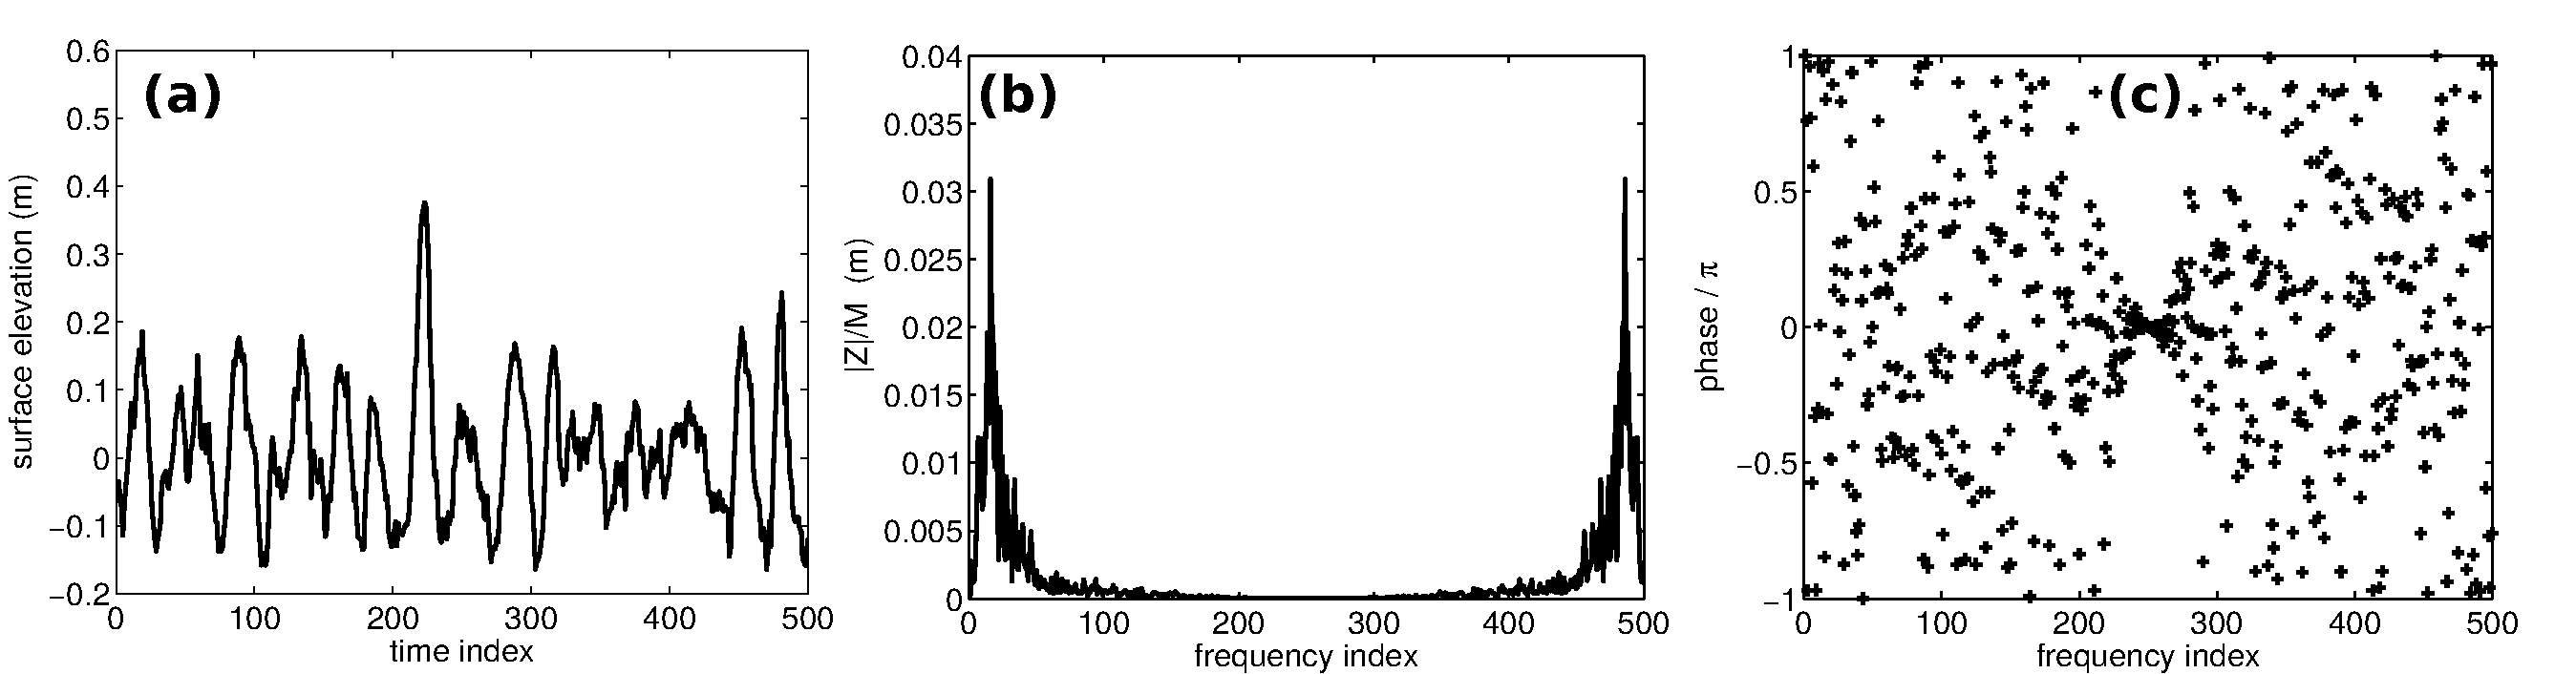
\includegraphics[width=0.9\textwidth]{FIGURES/spectra_DFT.pdf}}
%\vspace{3.64in}
\caption{(a) Example of surface elevation time series sampled at 12~Hz, (b) Discrete Fourier transform amplitude of the signal, and (c) phase of the same signal.} \label{fig:anaspec:spectreDFT}
\end{figure}
%%%%%%%%%%%%%%%%%%%%%%%%%%%%%%%%%%%%%%%%%%%%%%%%%%%%%%%%%%%%%%%%%%%%%%%%%%%%

With the definition given by eq. (\ref{eq:Zm_def}),  $Z_m=
\overline{Z_{M+2-m}}$, where the overbar is the complex conjugate, so that the modululs of the spectrum is symmetric around  $m=M/2$. This index $M/2$ corresponds to the Nyquist frequency 
$f_N=f_s/2 = M/2 df$. The symmetry means that above $f_N$ there is no new information. In other words, $f_N$ is the highest resolvable frequency. At this Nyquist frequency, a cosine wave is only represented by 2 points over a period. 

%We note that for stationary random variables that are quadratically integrable, i.e. all practical physical signals, the ratio $dZ(m) \overline{dZ(m)} / df$ goes to %$F(f)$ when $M$ goes 
%to infinity, i.e.  $f_s$ goes to zero, provided that  we keep constant 
%$f=(m-1)f_s/N$.  The increment
%$df=f_s/(N-1)$ is the spectral resolution, namely the frequency difference that can be resolved. The inverse of this resolution 
%$1/df$ is equal to the length of the recorded signal.

The continuous spectral density   $F(f)$ is obtained in the limit when the spectral resolution $df$ goes to zero of the following expression
\begin{equation}
    F(f=(m-1)f_s/M)  = 2  \frac{Z_m \overline{Z_m}}{df}.
\end{equation}
The factor 2 comes from the combination of positive and negative frequencies in the interval  $[0,  f_N]$. That definition is 
called the  single-sided spectrum. For some applications it may be convenient to keep the double-sided spectrum defined without this factor 2, 
for $f$ in the range $[0 , 2 f_N]$ or $[-f_N ,  f_N]$. 
In practice, the zero spectral resolution is never achieved because it corresponds to an infinitely long record. We are therefore stuck to finite 
spectral resolutions $df$, and thus a discrete spectrum sampled at $df$, corresponding to record lengths over which the random variable of interest is stationary. 


\subsection{Co-spectra}
In the same manner, we can  define the co-spectrum of two variables $a$ and $b$ having Fourier transforms $dA$ and $dB$, 
\begin{equation}
    C_{ab}(f=(m-1)f_s/M)  = \frac{A_m \overline{B_m}}{df} = P(f) +\mathrm{i}Q(f),
\end{equation}
where $P$ and $Q$ are real numbers, the co-spectra in phase and quadrature. 

We note that the product of two Fourier transforms is the Fourier transform of the convolution of the two functions. When these two functions are the same,
this result tells us that the spectrum is the Fourier transform of the auto-correlation function. When the two functions are different, the co-spectrum
is the Fourier transform of the correlation function. 

\section{Spectra from time series}
\subsection{Filtering of data and aliasing}
For any physical
parameter, the complex amplitude at a frequency above $f_N$ is the complex conjugate of the amplitude at a frequency below $f_N$: $dZ(N-m)=\overline{dZ(m)}$. 
In other words, the energy above the Nyquist frequency is aliased at  lower frequencies. This is one reason for applying a low-pass filter before the Fourier transform, in order to remove signals that would otherwise be aliased. 


%Il faut toujours bien r�fl�chir � la mani�re dont les donn�es sont filtr�es avant leur 
%�chantillonnage. Quand on mesure des vitesses toutes les dix minutes, est-ce une mesure instantan�e 
%une moyenne sur une, deux ou dix minutes? En effet les vitesses mesur�es contiendront alors 
%le courant moyen (par exemple caus� par la mar�e) mais aussi, si aucune moyenne n'est faite, les 
%fluctuations associ�es aux vagues et qu'il peut �tre tr�s d�licat de supprimer a post�riori. 

For example, a signal of period 1~s sampled every second ($f_s = 1$~Hz) is constant.  In general, any signal with frequency higher 
than the Nyquist frequency gives an apparent frequency in the range 
$[0 f_s/2]$, with a value obtained by folding back the spectrum along a vertical line at  $f=f_s/2$ or $f=0$ as many times as necessary, until 
 falling in $[0 f_s/2]$. Figure \ref{aliasing} shows an example of a true signal (in red) with frequency at  9/10 which gives  1-9/10=1/10 by aliasing. 
This is well known problem in oceanography in the case of the measurement of tides from satellite data. 
In the case of ocean waves, it is really necessary to measure waves with a sampling frequency that is at least 4 times the dominant frequency.  
%%%%%%%%%%%%%%%%%%%%%%%%%%%%%%%%%%%%%%%%%%%%%%%%%%%%%%%%%%%%%%%%%%%%%%%%%%%%
\begin{figure}[htb]
\centerline{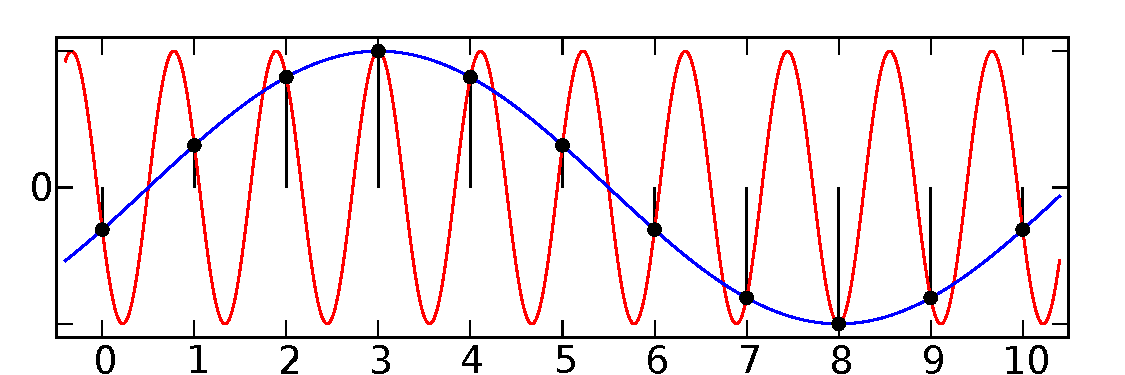
\includegraphics[width=0.5\textwidth]{FIGURES/AliasingSines.pdf}}
%\vspace{3.64in}
\caption{Example of spectral aliasing. A signal with period 10/9, in red, and sampled with a step of 1 (black dots) 
gives an apparent period of  10, in blue. (Moxfyre, wikimedia commons).} \label{aliasing}
\end{figure}
%%%%%%%%%%%%%%%%%%%%%%%%%%%%%%%%%%%%%%%%%%%%%%%%%%%%%%%%%%%%%%%%%%%%%%%%%%%%

In practice the high frequency roll-off of the wave spectrum, for $f > f_p$ in particular for pressure or velocity at the ocean floor, means that this 
filtering may not be necessary for the surface elevation. 
Figure \ref{fig:anaspec:timeseries} shows an example of the filtering of a surface elevation record and its impact on the spectrum. Here the filter helps in reducing 
the noise associated with the measurement method. 
%%%%%%%%%%%%%%%%%%%%%%%%%%%%%%%%%%%%%%%%%%%%%%%%%%%%%%%%%%%%%%%%%%%%%%%%%%%%
\begin{figure}[htb]
\centerline{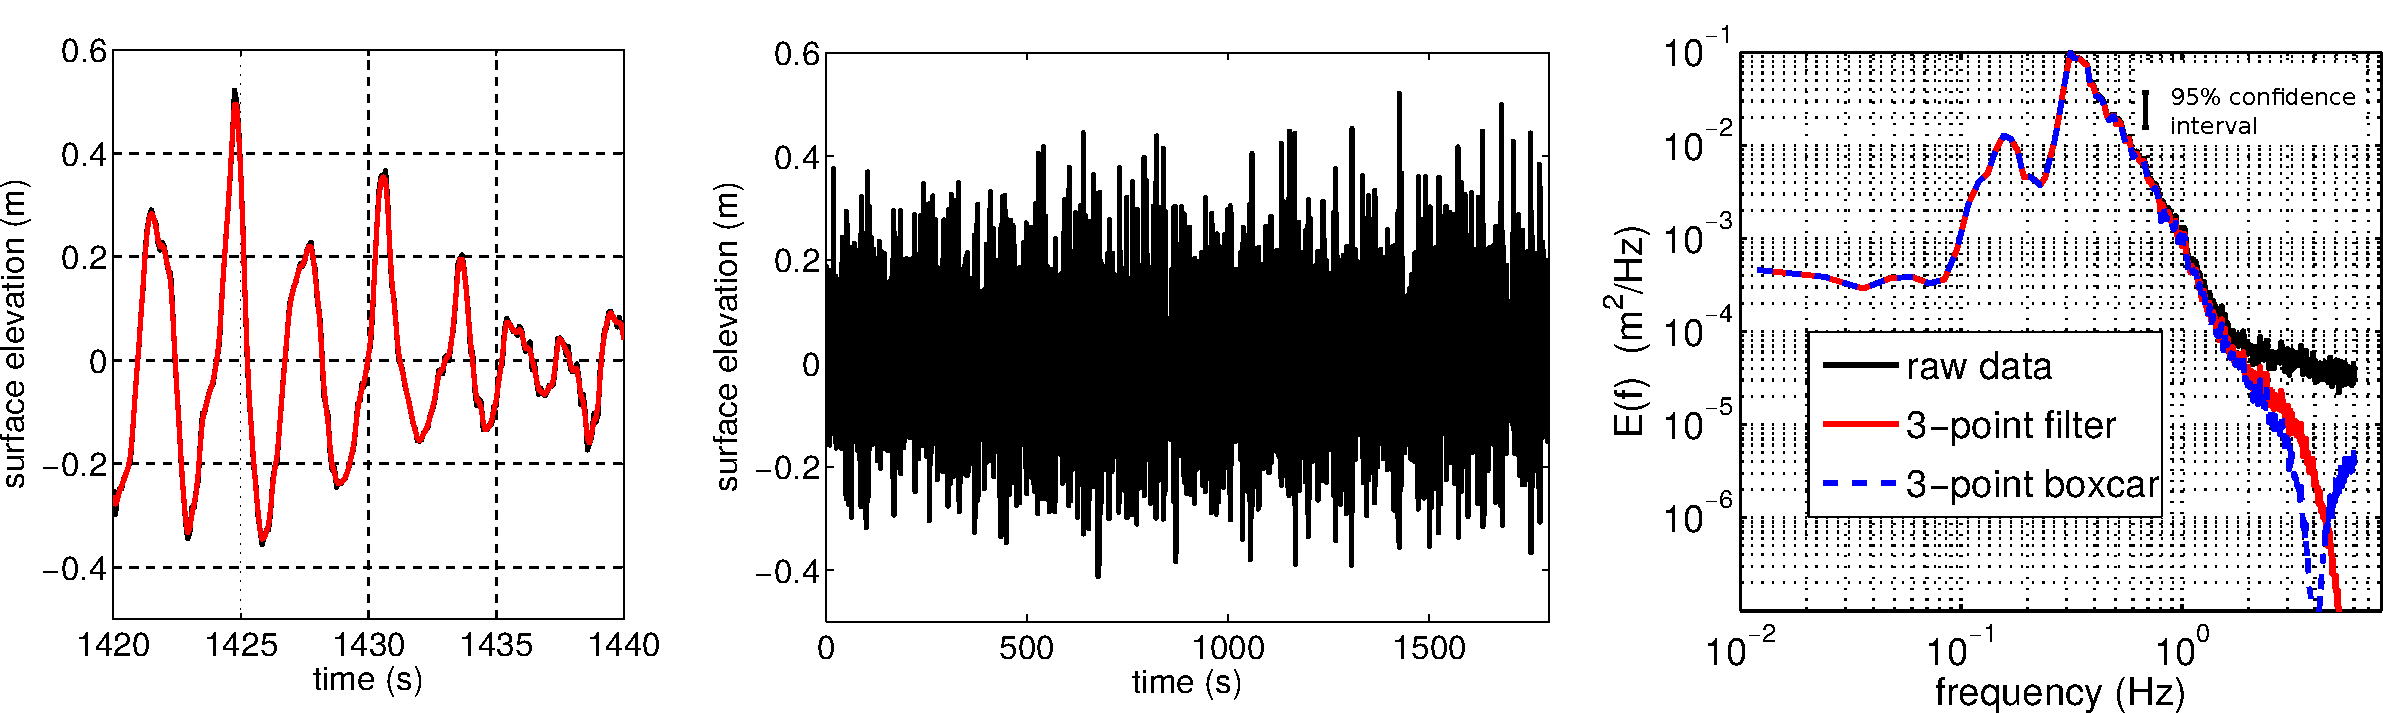
\includegraphics[width=\textwidth]{FIGURES/timeseries.pdf}}
%\vspace{3.64in}
\caption{Example of surface elevation measured by stereo-video from the Katsiveli platform, in 20~m depth, on Octoebr 4, 2011 \citep[see][for further detailed analysis of this dataset]{Leckler&al.2015,Aubourg&al.2017}.  (a) small piece of record around $t= 1430~s$ with (red) and without (black) a 3-point smoothing filter  (b) full record (1780~s) (c) spectra of the time series with different filters applied.} \label{fig:anaspec:timeseries}
\end{figure}
%%%%%%%%%%%%%%%%%%%%%%%%%%%%%%%%%%%%%%%%%%%%%%%%%%%%%%%%%%%%%%%%%%%%%%%%%%%%
The worst filter is clearly the boxcar (or moving average) filter with equal weight given to the consecutive data values, this does not suppress very well the shortest components.  


\subsection{Windows, Gibbs phenomenon and averaging}
The discrete Fourier transform of signal $\zeta$ that takes values at locations 1 to N, corresponds to the Fourier transform of a periodic signal that would 
repeat itself with $\zeta(n+m M) = \zeta (n)$ for any $n$ and $m$. If 
$\zeta(1)\neq \zeta(M)$, then this periodic function has a sharp jump from $\zeta(M)$ to $\zeta(M+1)$. Such a jump 
can give a strong spectral signature, all across the spectrum. 


This artifact is known as the Gibbs phenomenon, and it 
is generally removed by multiplying the signal  $\zeta(n)$ by a window function $W(n)$ which goes to zero or very small values for both 
$n=1$ and $n=N$. Obviously the spectrum of $\zeta(n) \times W(n)$ is different from the spectrum of $\zeta(n)$. The first obvious effect is that 
the variance of the signal has been reduced by a factor that is the average of $W^2$. That is easily corrected for.




Let use the time series shown in figure \ref{fig:anaspec:timeseries}.b. We first start with a small piece of only 1000 points. The original time series, in black 
in figure \ref{fig:anaspec:spectre1}.a gives the power spectral density in figure {fig:anaspec:spectre1}.b. If the time series is brought to zero at both ends (in red) by multiplying with a Hann window, then the spectrum is transformed. However, because of the random fluctuations of the spectral estimates this is not obvious.
Indeed waves are random and the surface elevation is nearly-Gaussian. As a result, the complex Fourier amplitudes are also random and Gaussian, so that they modulus, which is the power spectral density has the shape of a  $\chi^2_n$ distribution with $n=2$ degrees of freedom. Because the $\chi^2_n$ distribution has a mean of $n$, the distribution of estimates $\widehat{E}(f)$ of the spectrum, once normalized by the mean spectrum $E(f)$ follows the rescaled $\chi^2_n$ disitribution, with a mean equal to 1. 

%%%%%%%%%%%%%%%%%%%%%%%%%%%%%%%%%%%%%%%%%%%%%%%%%%%%%%%%%%%%%%%%%%%%%%%%%%%%
\begin{figure}[htb]
\centerline{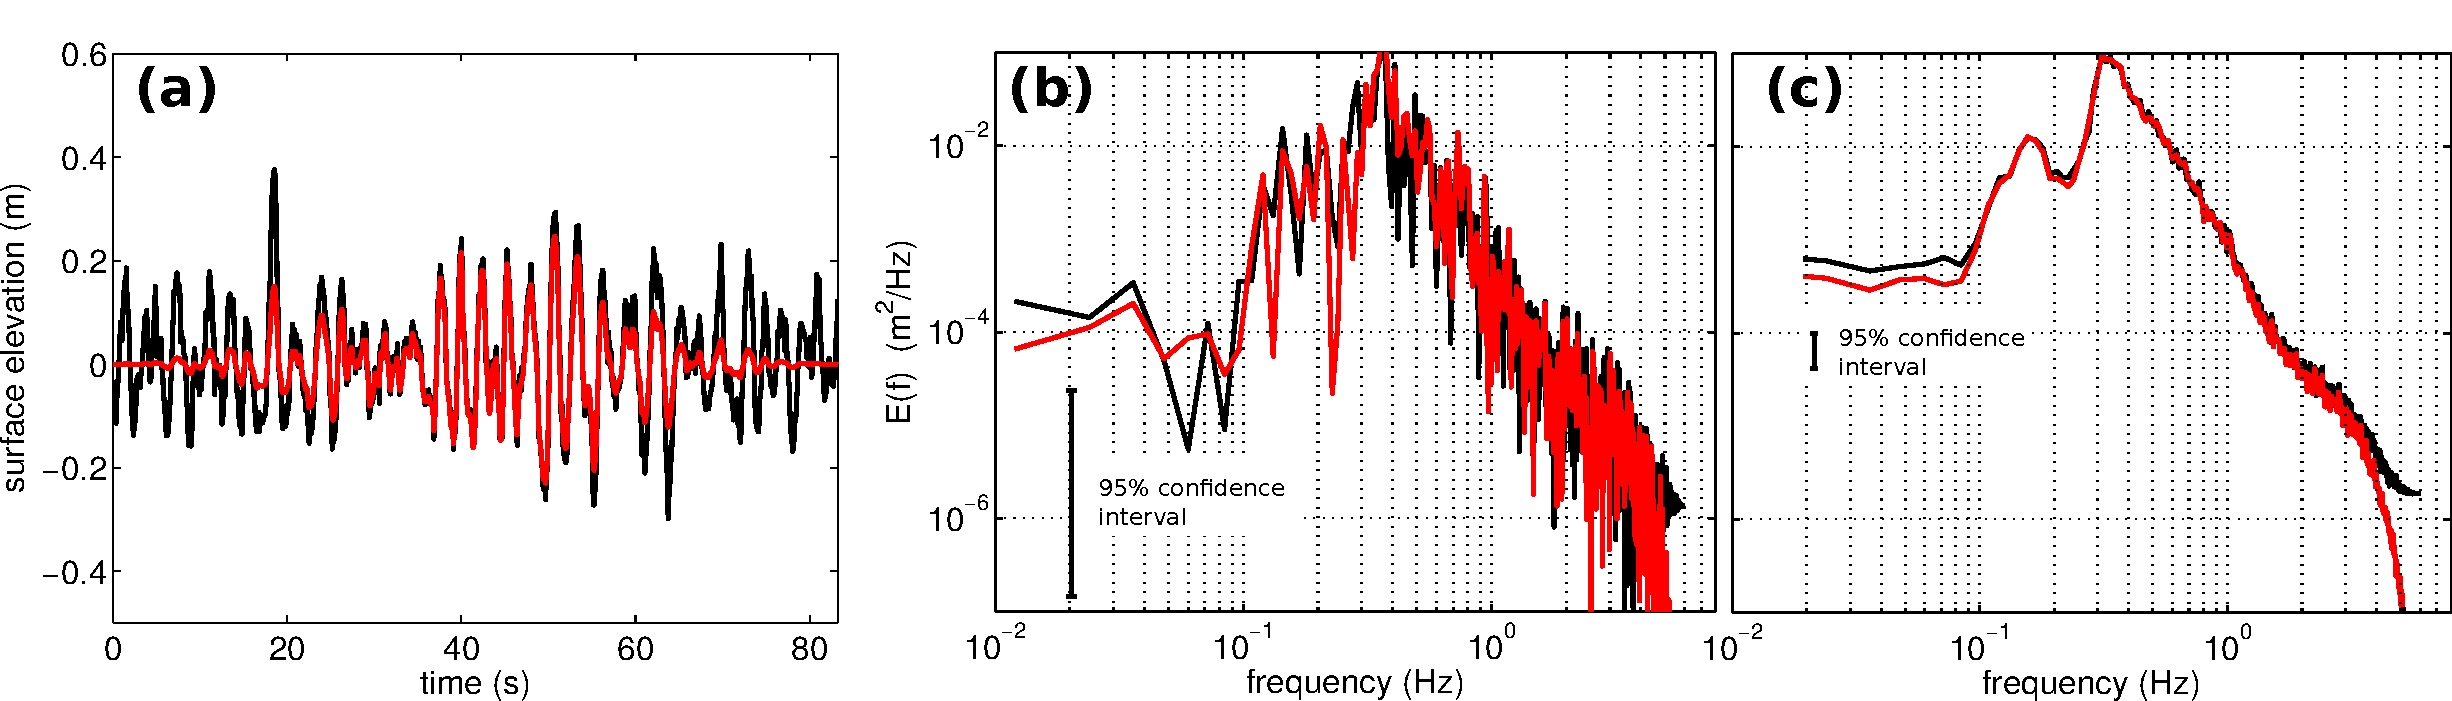
\includegraphics[width=\textwidth]{FIGURES/spectra1.pdf}}
%\vspace{3.64in}
\caption{(a) First 1000 points of time series shown in  (\ref{fig:anaspec:timeseries}).b, with (red) and without (black) multiplication by a Hann window. 
(b) Resulting spectra (c) Average spectra using Welch's method with 21 independent windows and thus 42 degrees of freedom.} \label{fig:anaspec:spectre1}
\end{figure}
%%%%%%%%%%%%%%%%%%%%%%%%%%%%%%%%%%%%%%%%%%%%%%%%%%%%%%%%%%%%%%%%%%%%%%%%%%%%
 Using figure \ref{table_chi2}, we find that the expected ratio of the lower and upper bound of a 95$\%$ confidence interval is 146. This number is the ratio of  $\chi^2_{2,0.975}$�and  $\chi^2_{2,0.025}$, that give the probabilities that $\chi^2_{n} > \chi^2_{n,\alpha}$ is equal to the acceptance threshold $\alpha$. 
%%%%%%%%%%%%%%%%%%%%%%%%%%%%%%%%%%%%%%%%%%%%%%%%%%%%%%%%%%%%%%%%%%%%%%%%%%%%
\begin{figure}
\centerline{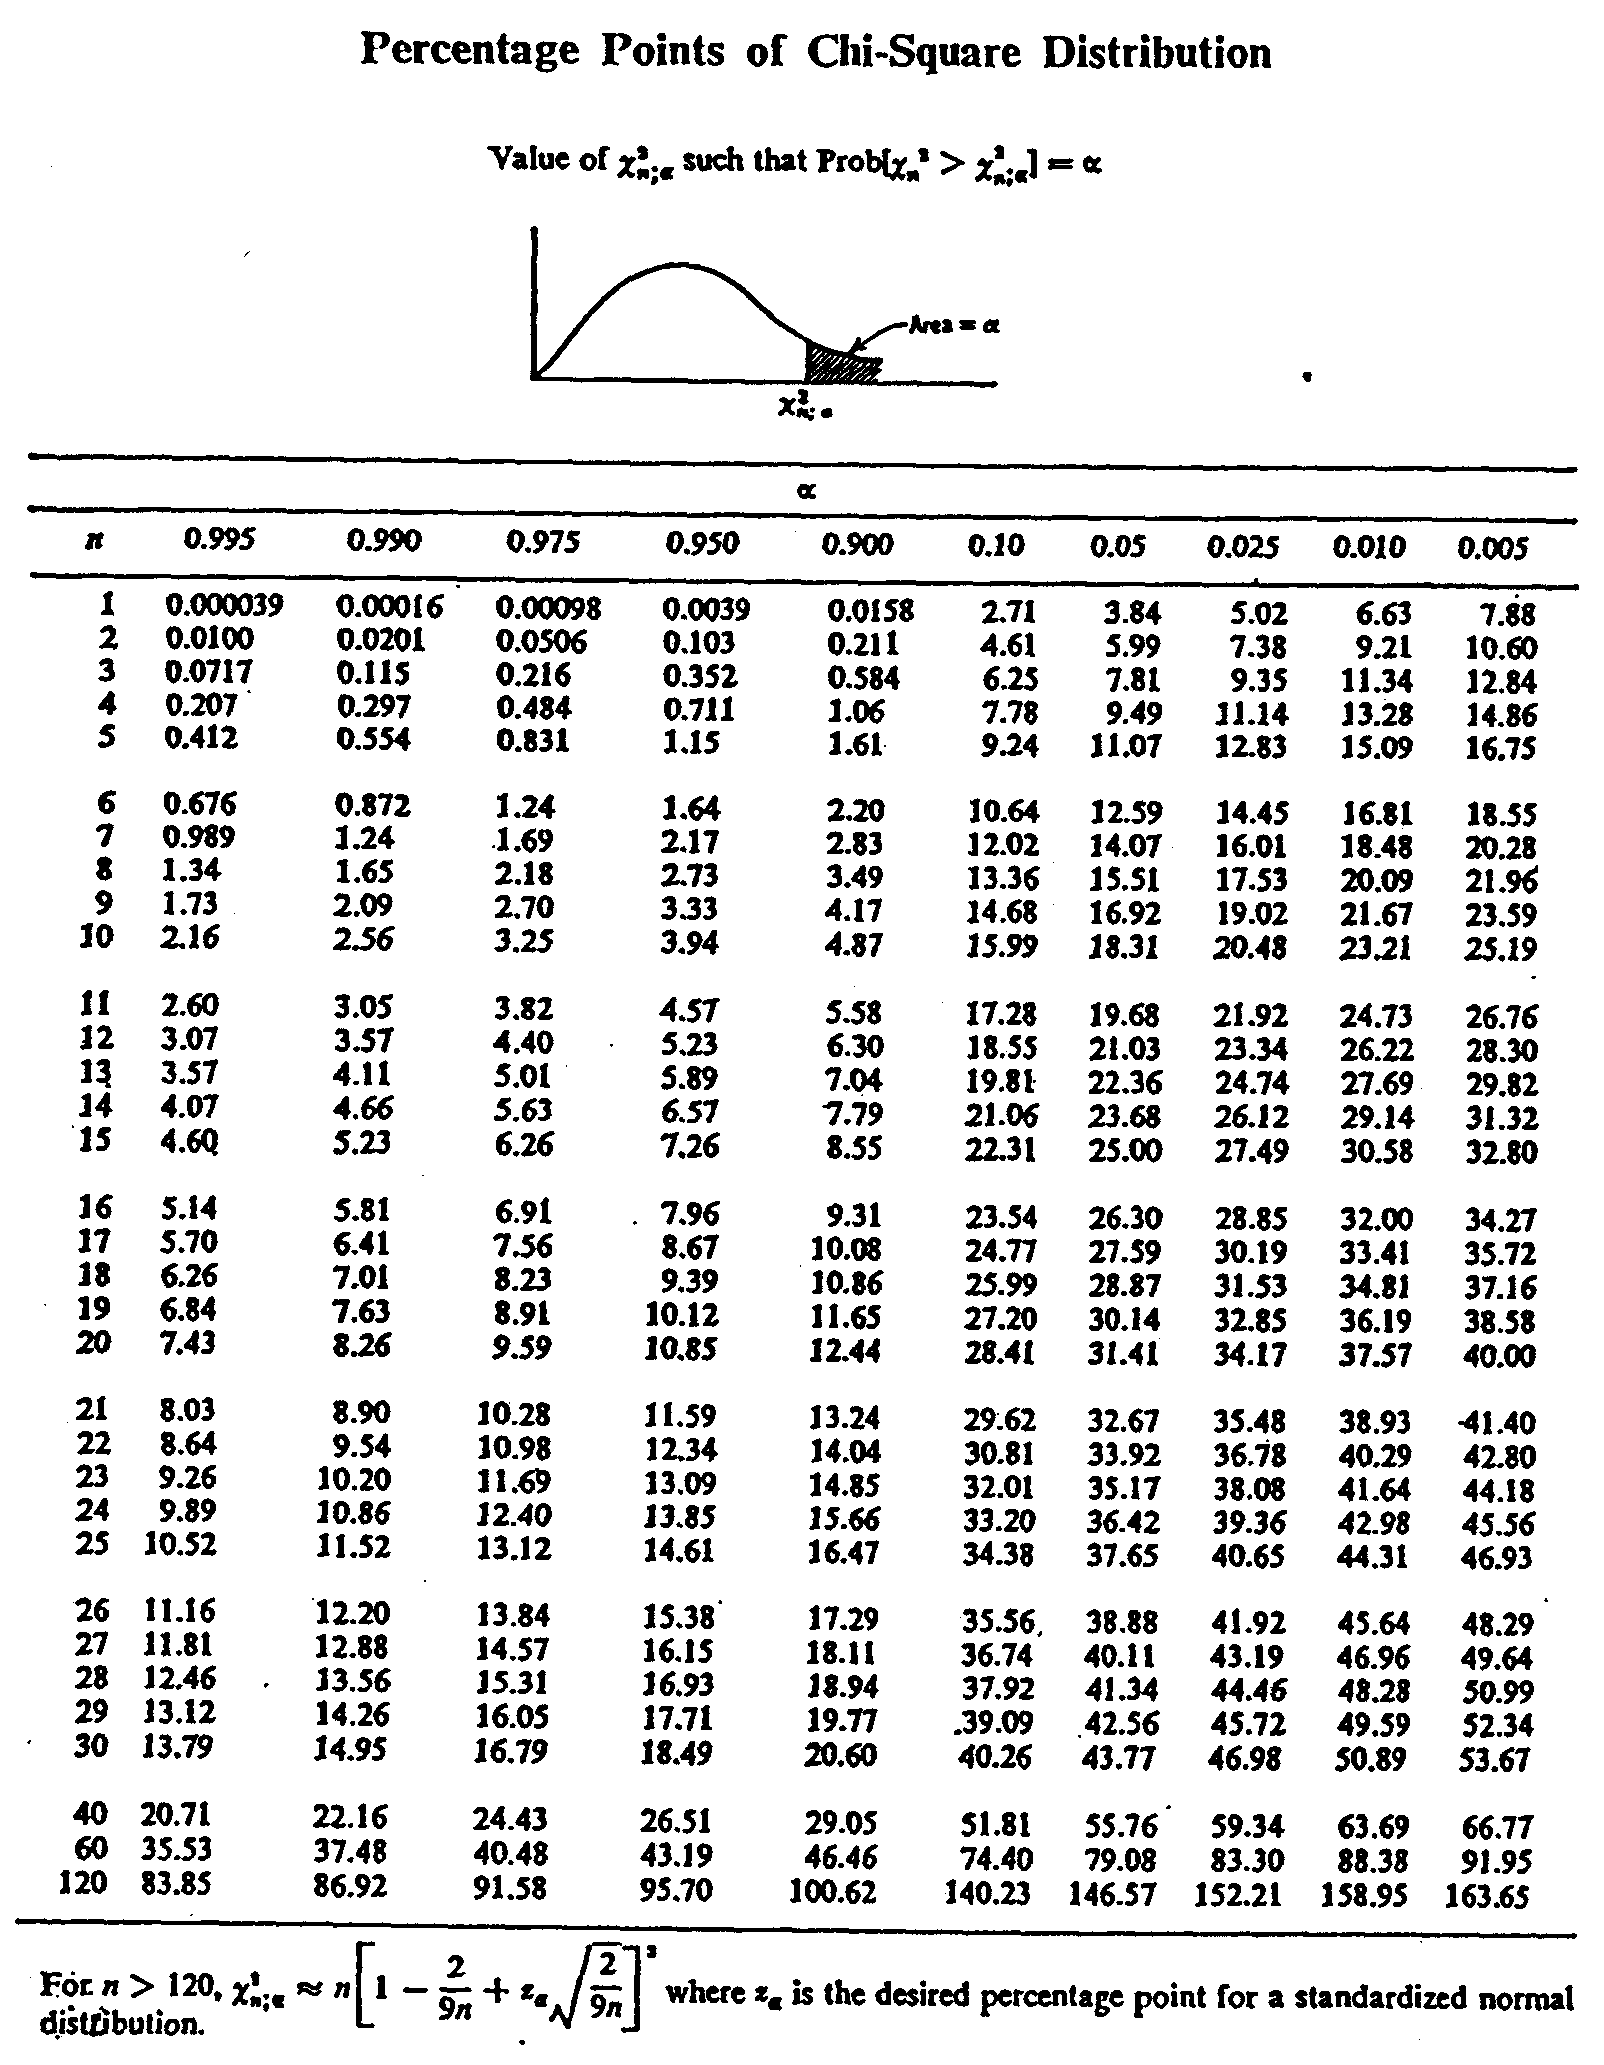
\includegraphics[width=\textwidth]{FIGURES/table_chi2.png}}
%\vspace{3.64in}
\caption{Table of $\chi^2$ distributions. This table gives the confidence intervals
for the estimation of spectra with 
$n=2 N$ degrees of freedom, where $N$ is the number of independent spectra used.} \label{table_chi2}
\end{figure}
%%%%%%%%%%%%%%%%%%%%%%%%%%%%%%%%%%%%%%%%%%%%%%%%%%%%%%%%%%%%%%%%%%%%%%%%%%%%


For an expected value  $\widehat{E}$, the  Gaussian statistics theory predicts a 95\% probability that the estimate of $E(f)$ is in the range $[E_1, E_2]$ with $E_1=\widehat{E} \times 0.0506/2 $ and  $E_2=\widehat{E} \times 7.38/2$, where 0.0506 and 7.38 are the values for which the $\chi^2$ cumulative probability function for 2 degrees of freedom is $\alpha=0.975$ and $\alpha=0.025$, respectively as given \ref{table_chi2}. In other words, the random fluctuations of the spectrum estimated by a single Fourier transform spans more than two orders of magnitude. 

That is fairly annoying. There are two ways to reduce this uncertainty: the first, which is most easily done in the laboratory is to run more experiments, repeating the same conditions, with random wave phases, and average the results. For measurements in the field, this is the same as processing a longer time series, but it only makes sense if the conditions are stationary: same wind, same wave age, same current, etc. In practice, this stationarity constraints limits the length of records from half an hour to a few hours. As we average $N$ spectra together, the number of degrees of freedom increases to $2N$. Here we have used 21 independent spectra, and we get an uncertainty that narrows like $1/\sqrt{N}$ for large $N$. For 20 spectra, the ratio $E_2/E_1$ is $59.34/34.43\simeq 1.7$. As $N$ increases, the spectral resolution becomes coarser.

Because the Hann window practically removes part of the data, \cite{Welch1967} has defined a method in which the windows are shifted by half their length, as shown in figure \ref{fig:anaspec:spectre31}.a. The lower panel shows the 21+20 spectra estimated, and the average result.  
%%%%%%%%%%%%%%%%%%%%%%%%%%%%%%%%%%%%%%%%%%%%%%%%%%%%%%%%%%%%%%%%%%%%%%%%%%%%
\begin{figure}
\centerline{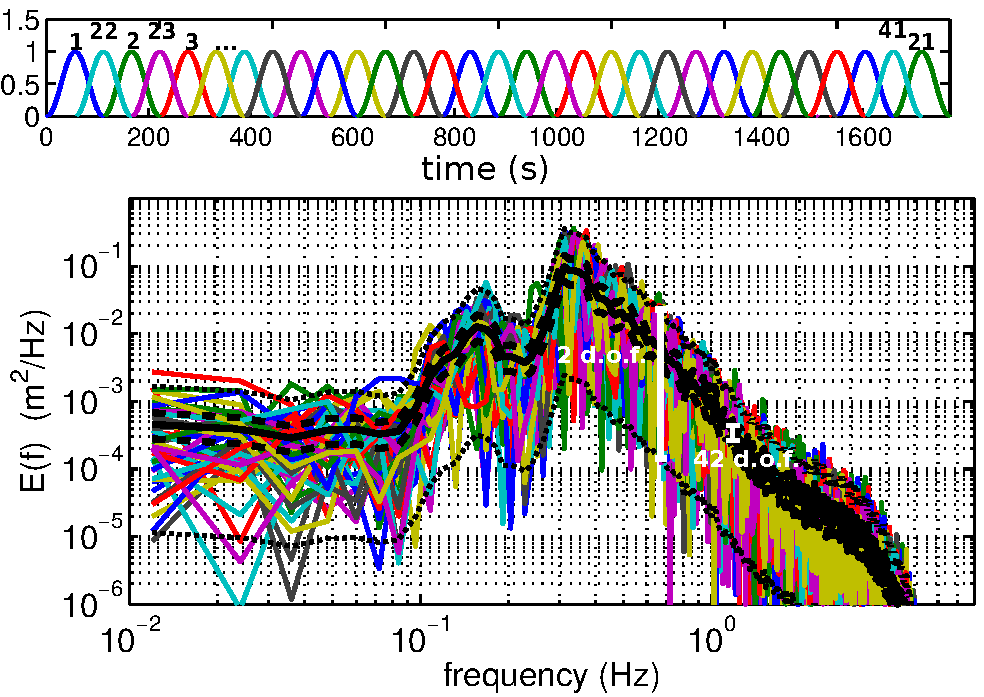
\includegraphics[width=0.9\textwidth]{FIGURES/spectra_31.pdf}}
%\vspace{3.64in}
\caption{(a) Succession of the Hann windows applied to the data, with 21 independent windows and 20 overlapping windows, from number 22 to 41. The solid line is the mean spectrum and the dotted and dashed line show the expected 95\% confidence intervals for 2 and 42 degrees of freedom. 
� 95\%.} \label{fig:anaspec:spectre31}
\end{figure}
%%%%%%%%%%%%%%%%%%%%%%%%%%%%%%%%%%%%%%%%%%%%%%%%%%%%%%%%%%%%%%%%%%%%%%%%%%%%

Another method that is almost equivalent to Welch's is the smoothing of the spectrum, also known as band-averaging. Because the Fourier transform of a shorter 
window has a coarser resolution, both methods effectively trade off the spectrum accuracy against the spectral resolution. An extension of such methods is the use of wavelet transforms \citep[e.g.][]{Liu&Babanin2004} which aims at localizing events in both time and frequency. 

Whatever the choice of method, without any prior knowledge on the signal, the product of the spectra uncertainty and the square root of the frequency uncertainty remains constant. Thus the optimal choice of $df$ is up to the user. For wind seas, the typical relative width of the spectrum is 0.1, and for a typical peak period of 0.1~Hz, resolving the peak requires $df < 0.01$~Hz. For swells one may like to have an even narrower frequency resolution.  In the example above, $df=0.012$~Hz is 
enough for the relatively short wind sea found in the Black Sea. 

\subsection{Interpretations and further developments}
The general idea of spectral analysis is to decompose a signal into its basic constituents. If waves were indeed linear, the Fourier components would be truly independent and the spectrum would give the energy of different wave components. In practice, there is a significant level of nonlinearity, which actually dominates the frequency spectrum $E(f)$ at frequencies above 3 to 4 times the wind sea peak \citep[e.g.][]{Leckler&al.2015}. As a result, the interpretation of these high frequencies ($f > 1$~Hz in the example above) as the energy of linear waves is wrong. Several methods have been developed to try to separate linear and non-linear components, including higher order analysis \citep{Hasselmann&al.1963} which is illustrated in chapter \ref{ch_surf}. This question has inspired other nonlinear methods, such as the Empirical Mode Decomposition method by \cite{Huang&al.1998}.


\section{Spectral analysis of directional buoy data}
\subsection{Case of 3-axis displacements or accelerations}
We have seen in section  \ref{sub:transfer} that the spectrum of $x$-component velocity  at the ocean bottom 
is given from the surface elevation spectrum multiplied by a transfer function,
\begin{equation}
    E_{Ux} \left( f,\theta \right)  = \frac{\sigma^2 \cos^2 \theta}{\sinh^2 (kD)} E\left( f,\theta
    \right)\label{EUX }.
\end{equation}
%et le module moyen de la vitesse (en moyenne quadratique) pr�s du fond vaut,
%\begin{equation}
%    U_{\mathrm{b,rms}} = \left[\int_0^{\infty} \int_0^{2 \upi} \frac{\sigma^2}{\sinh^2
%    (kD)} E\left( f,\theta \right){\mathrm d}\theta
%    {\mathrm d}f \right]^{1/2}
%\end{equation}

The same method applies to spectra of displacements, velocity and slopes at the sea surface. 
For a water particle at the surface, the spectra of displacement in the three directions are given by  (\ref{xi3}),
\begin{eqnarray}
    E_{x} ( f)  & = &  \frac{1}{\tanh^2(kD)} \int_0^{2 \upi} E\left( f,\theta \right)\cos^2 \theta {\mathrm
    d}\theta \\
    E_{y} ( f)  & = &  \frac{1}{\tanh^2(kD)} \int_0^{2 \upi} E\left( f,\theta \right)\sin^2 \theta {\mathrm
    d}\theta \\
   E_{z} ( f)  & = &  \int_0^{2 \upi} E\left( f,\theta \right) {\mathrm
    d}\theta.
\end{eqnarray}
We note that this last spectrum is the usual elevation spectrum $E(f)$, also called heave spectrum, with a minor modification due to the fact that it is not 
obtained at a fixed position $(x,y)$ but at a positions that moves with $x$ and $y$. As a result, the shape of the waves and the shape of the spectrum are modified, with a strong reduction in the contribution of nonlinear harmonics: a surface buoy signal looks much more linear than a wave staff or stereo video record. 

The co-spectra of horizontal and vertical displacements are 
\begin{eqnarray}
    C_{xz} ( f)  & = &  \frac{\mathrm i}{\tanh(kD)} \int_0^{2 \upi} E\left( f,\theta \right)\cos \theta {\mathrm
    d}\theta, \label{Exz}\\
    C_{yz} ( f)  & = &  \frac{\mathrm i}{\tanh(kD)} \int_0^{2 \upi} E\left( f,\theta \right)\sin \theta {\mathrm
    d}\theta .\label{Eyz} \\
    C_{xy} ( f)  & = &  \frac{1}{\tanh^2(kD)} \int_0^{2 \upi} E\left( f,\theta \right)\sin \theta \cos \theta {\mathrm
    d}\theta .\label{Exy}
\end{eqnarray}
These co-spectra are thus related to the mean direction and directional spread, through the directional moments introduced in section  \ref{sub:param}
\begin{eqnarray}
    a_1 ( f)  & = &  \int_0^{2 \upi} E\left( f,\theta \right)\cos \theta {\mathrm
    d}\theta, \\
    b_1 ( f)  & = &   \int_0^{2 \upi} E\left( f,\theta \right)\sin \theta {\mathrm
    d}\theta,  \\
    a_2 ( f)  & = &  \int_0^{2 \upi} E\left( f,\theta \right)\cos (2\theta) {\mathrm
    d}\theta, \\
    b_2 ( f)  & = &   \int_0^{2 \upi} E\left( f,\theta \right)\sin (2 \theta) {\mathrm
    d}\theta.
\end{eqnarray}


To summarize, starting from the displacement time series  $x(t)$, $y(t))$ and $z(t)$ one obtains the 
spectra and co-spectra  $C_{xx}(f)$,  $C_{yy}(f)$,  $C_{zz}(f)$,  $C_{xz}(f)$, $C_{yz}(f)$ , $C_{xy}(f)$.
Using $\cos(2 \theta)=\cos^2(\theta) - \sin^2(\theta)$ and $\sin(2 \theta)=2 \sin \theta \cos\theta$, they give the following directional moments, in which $\Im $ stands for the imaginary part, 
\begin{eqnarray}
  a_1 ( f) &=&-\Im (C_{xz}(f))/\left[C_{zz}(f) \left(C_{xx}(f)+C_{yy}(f)\right)\right] \\
  b_1 ( f) &=&-\Im (C_{xy}(f))/\left[C_{zz}(f) \left(C_{xx}(f)+C_{yy}(f)\right)\right] \\
  a_2 ( f) &=&(C_{xx}(f)-C_{yy}(f))/(C_{xx}(f)+C_{yy}(f)) \\
  b_2 ( f) &=&2 C_{xy}(f) /(C_{xx}(f)+C_{yy}(f))  \\
\end{eqnarray}
from which we get directional parameters, with $\mod$ the modulo operator, 
\begin{eqnarray}
  \theta_{1}(f) &=&  \mod( 270.- \mathrm{atan2}(b1,a1)\times 180/\pi, 360)\\
  \sigma_{1}(f)&=&\left[2\left(1 - \sqrt{a_1^2(f) + b_1^2(f)} \right)\right]^{0.5}\times 180/\pi \\
  \theta_{2}(f) &=&  \mod( 270.- 0.5 \mathrm{atan2}(b2,a2)\times 180/\pi, 360)\\
  \sigma_{2}(f)&=&\left[0.5\left(1 - \sqrt{a_2^2(f) + b_2^2(f)} \right)\right]^{0.5}\times 180/\pi
\end{eqnarray}


These 4 parameters can be used in statistical estimators to obtain the directional spectrum $E(f,\theta)$. A commonly used estimator 
is the Maximum Entropy Method of \cite{Lygre&Krogstad1986}. See also the review by \cite{Benoit&al.1997}.

\subsection{Case of other systems with 3 variables or more}
in the above method, we can replace $x$ and $y$ by the slopes $\partial \zeta / \partial x$  and $\partial \zeta / \partial y$ as done in the pitch-and-roll buoys 
developed by \cite{Cartwright&Smith1964} and still widely used. For example, most of the 3-m discuss buoys operated by the U.S. National Data Buoy Center are based 
on this measurement \citep{Steele&al.1992}. Also, the horizontal 
velocities at any given level, $(u,v)$. These give access to the heave spectrum $E(f)$ and the same directional moments $a_1$, $b_1$, $a_2$ and $b_2$. 

In order to go beyond these first 5 parameters, one can built an array of instruments. The cloverleaf buoy of \cite{Mitsuyasu&al.1975} was such an attempt, and arrays of pressure gages or lasers have been routinely used. Today's optical techniques \citep{Benetazzo2006,Fedele&al.2013,Laxague&al.2015} are other ways to get to more details about the sea surface.


\section{Some links between spectral and wave-by-wave analysis}
The spectrum $E(f)$ gives the distribution of the surface elevation variance as a function of time scales. As discussed in chapter \ref{ch1}, one can also chop the 
signal in individual waves and study the statistics of their properties. 
A model for the sea surface elevation could be a signal of constant amplitude with a random frequency modulation. In that case, \cite{Woodward1952}'s theorem 
tells us that the spectrum of the signal is the distribution of its frequencies $P_f(f-f_c)$ where $f_c$ is the carrier frequency,
\begin{equation}
    E(f) = \frac{a^2}{2}P_f(f-f_c).
\end{equation}

Extension of that theorem by \cite{Blachman&McAlpine1969} with an additional amplitude modulation makes it applicable to ocean waves.  As  shown by  \cite{Elfouhaily&al.2003} the spectrum is then given by the joint probability distribution of wave heights and periods $P(a,f)$ with $a=H/2$ and $f=1/T$. 
Separating linear (naked) and full (dressed) spectra, \cite{Elfouhaily&al.2003} showed that the peak region is dominated by linear components 
\begin{equation}
    E_{\mathrm bare}(f) = \frac{1}{2}\int a^2 P(a,f) da.
\end{equation}

At high frequency the nonlinear contributions dominate the spectrum which can be interpreted as fast modulations of the short components. Taking into account that 
effect leads to asymetries $\alpha$ et $\beta$
(see figure \ref{Asymetrie_Elf}), and the dressed spectrum
\begin{equation}
    E_{\mathrm{dressed}}(f) =  E_{\mathrm nu}(f) +\frac{1}{2}\left[ \int \alpha^2 P(\alpha,f/2)
    da+ \int \beta^2 P(\beta,f/2) da\right] \simeq E(f)
\end{equation}
%%%%%%%%%%%%%%%%%%%%%%%%%%%%%%%%%%%%%%%%%%%%%%%%%%%%%%%%%%%%%%%%%%%%%%%%%%%%%%%%%%%%%
\begin{figure}
\centerline{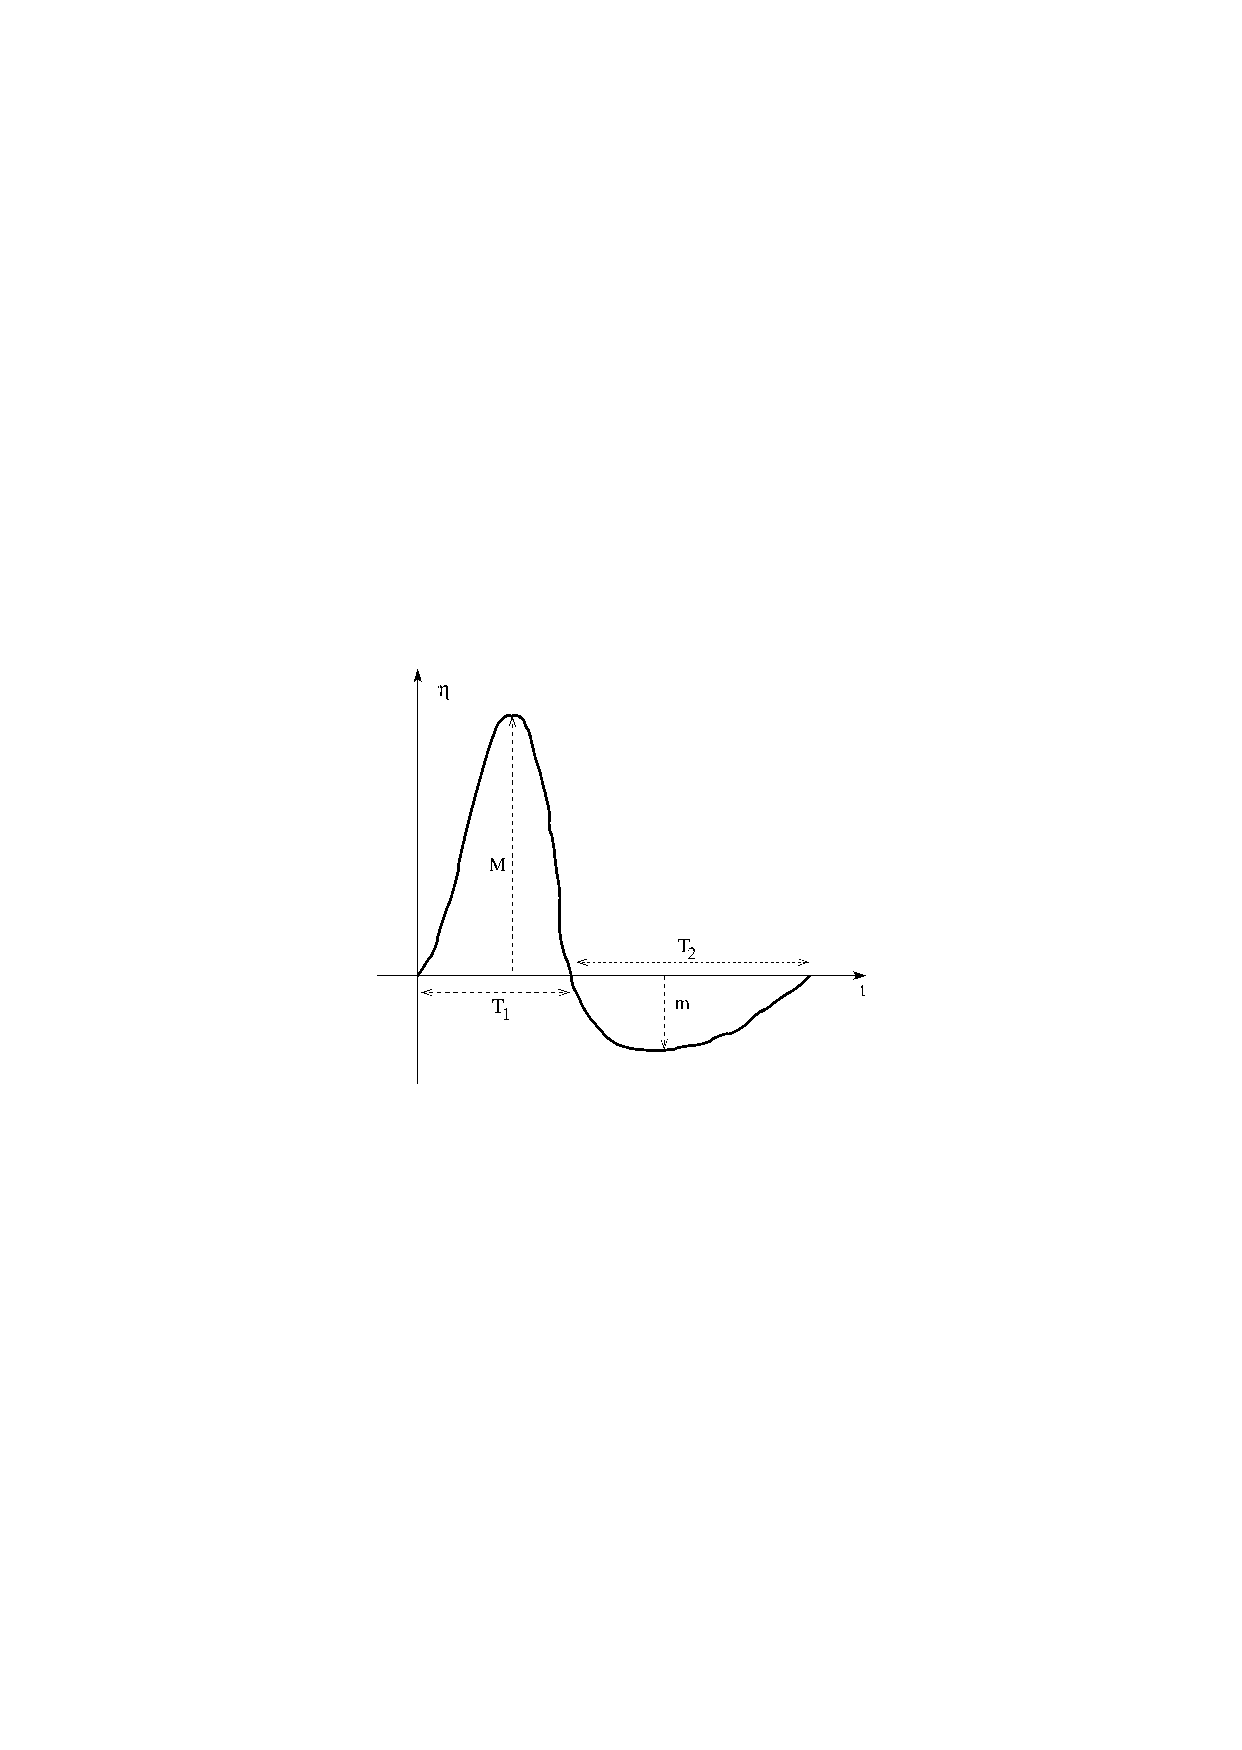
\includegraphics[width=0.6\textwidth]{FIGURES/Asymetrie_Elf.pdf}}
%\vspace{3.64in}
  \caption{Definition of parameters $M$ ,$m$, $T_1$ et $T_2$ used to estimate the amplitude  $a=(M-m)/2$, period $T=T_1+T_2$, vertical asymetry  $\alpha=(M+m)/2$  and horizontal asymetry $a\pi(T_1-T_2)/(T_1+T_2)/2$ (from \cite{Elfouhaily&al.2003}, \copyright Elsevier).
   Here $m<0$, because $m$ is defined as the trough level between two up-crossing zeros that define the start and end of the wave.} \label{Asymetrie_Elf}
\end{figure}
%%%%%%%%%%%%%%%%%%%%%%%%%%%%%%%%%%%%%%%%%%%%%%%%%%%%%%%%%%%%%%%%%%%%%%%%%%%%%%%%%%%%%%%%%%%



\cleardoublepage
\chapter{Wave groups and fluctuations of wave parameters}\label{ch_groups}
Before we look at the evolution of the wave field over tens of kilometers and hours time scale, it is 
worth looking at consequences of the shape of the wave spectrum 
on fluctuations in wave properties at the scale of few minutes and kilometers.
Indeed, the fact that waves are random introduces small scale variations. Most early work 
was focused on defining the statistics of series of high waves \citep{Arhan&Ezraty1978,Masson&Chandler1993}, which can be useful for example when catching 
waves on a surfboard, avoid the high waves when navigating a landing craft through the surf zone, or landing a helicopter on a ship. In this 
chapter we will start with another application which has become prominent as we are 
starting to look at smaller and smaller scale details in the wave field: estimating the expected 
fluctuations associated with groups \citep{DeCarlo&al.2023}, so that we may separate it from other effects, including 
refraction induced by currents and water depth, wave breaking, etc, which will be discussed in the 
following chapters. This investigation will also allow us to estimate lower bounds for uncertainties 
of wave measurements that will be defined from the time and space footprint of t{he measurements. The full uncertainty also contains instrument noise and measurement noise effects.

\section{Wave envelope, local amplitudes and their statistics}

Let $\zeta_c$ be the complex number such that $\zeta = \mathrm{Re}(\zeta_c)$ is the free surface, $\zeta_c$  is usally called the analytic signal. The envelope $\eta$ of the signal is defined by  $\eta = |\zeta_c|$, with an example shown in Fig. \ref{fig:groups1D}, using bottom pressure $p(z=-h)$ instead of surface elevation $\zeta$. 
%%%%%%%%%%%%%%%%%%%%%%%%%%%%%%%%%%%%%%%%%%%%%%%%%%%%%%%
\begin{figure}[htb]
\centerline{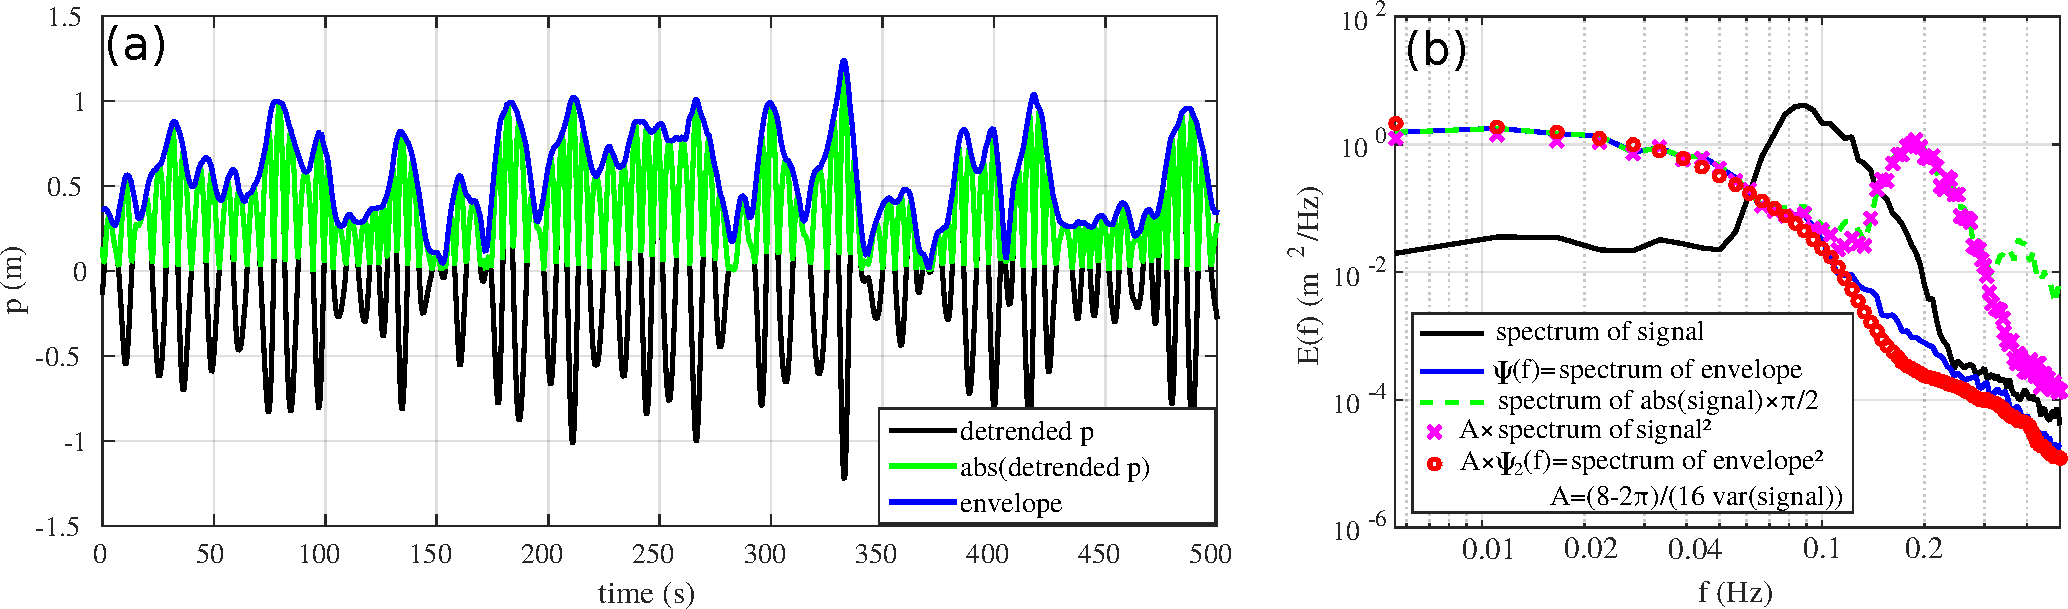
\includegraphics[width=\textwidth]{FIGS_CH_GROUPS/envelope_1D.pdf}}
%\vspace{3.64in}
  \caption{(a) time series of a signal, here the detrended ocean bottom pressure in Berthaume on January 31st 2004 (same data as in Figure 1.2), absolute value of the signal and signal envelope. (b) Spectra of the signal, the envelope, the rectified signal, and the approximate spectrum $\Psi_2$ obtained from a spectral convolution.}
\label{fig:groups1D}
\end{figure}
%%%%%%%%%%%%%%%%%%%%%%%%%%%%%%%%%%%%%%%%%%%%%%%%%%%%%%%
This defines a local amplitude of the signal that is continously defined everywhere. One interesting property of the envelope is that it does not contain the small scale crest-to-trough (positive to negative) variations of the original surface, so that its spectrum actually contains only longer components (larger periods in the case of time series). It is interesting to note that a similar operation is obtained by \emph{rectifying} the signal, i.e. taking its absolute value. This was particularly studied for electric signals by \cite{Rice1944} and the \emph{rectifier} in that case is a simple diode bridge. In the case of ocean waves, an important application is that of forces on moored ships, and you can think of the mooring line as a kind of rectifier, which will thus endure low-frequency forces. 

In fact it is easy to show that the signal and the rectified signal have the same mean squared value (i.e. the same integral of the spectrum including $f=0$), but they have very different spectra: the mean squared of the rectified signal is actually split half and half between sub-harmonics (very low frequencies) and super harmonics (higher than the peak frequency). Because the mean envelope squared is twice the mean rectified signal squared (if it is not obvious, think about it), then the envelope spectrum happens to be 4 times the spectrum of the rectified signal at low frequencies. 

The spectrum of the envelope turns out to be a pretty important quantity for many applications. Indeed, any non-linear effect will typically give the same kind of sub-harmonic and super-harmonic. In particular, any measurement device that is weakly non-linear will produce  spurious large scale fluctuations: this is the case of mooring lines for floating buoys, it is also the case of the KaRIN radar on board the SWOT satellite \citep{Peral&al.2015}. Separating the spurious signal from the real signal can involve the spectrum of the envelope. So you may be pleased to know that we can compute the spectrum of the envelope from the wave spectrum itself using the following approximation \citep{Tayfun&Lo1989}
\begin{equation}
    \Psi \simeq \frac{8 - 2\pi}{H_s^2}  \Psi_{2},
\label{eq:TayfunetLo}
\end{equation}
where $\Psi_2$ is the spectrum of the envelope squared and is obtain by convolving the wave spectrum with itself. This expression is valid for the surface elevation envelope. For any other quantity (orbital velocity, Stokes drift ...), just replace $H_s$ by 4 times the standard deviation of the quantity of interest. And before you complain that this is only an approximation, you may note that we have an exact equation for the spectrum of the envelope squared: if you enjoy the satifying beauty of exact equations please consider studying the fluctuations of the variances instead of the fluctuations of the amplitudes, and things will be very nice. 

We will now use this envelope spectrum to compute the expected fluctuations of wave measurements when estimated from a short record or a small area: here "short" or "small" is relative to the size of a few wave groups in time and space. The concept is the same when working with time series or two-dimensional maps, so we will treat both situations, starting with time series. 

\subsection{Time series}
From a time series $\zeta(t)$, the envelope can also be defined using the  Hilbert transform $\cal{H}(\zeta)$ of the time series, 
\begin{equation}
   \eta  = \left| \zeta + \cal{H}(\zeta) \right|.
   \label{eq:env_Hilbert}
\end{equation}
A practical calculation of the Hilbert transform is obtained using Fourier and inverse Fourier transforms. 


\subsubsection{Definition of a local wave height}
From the envelope $\eta$ we define the wave height $H_{r}$ as an average over a time segment of "radius" $\tau$
\begin{equation}
    H_{\tau}(t) = 4\sqrt{\frac{2}{\pi}} (\eta \otimes g_{\tau})(t)
   \label{eq:relation_Hs_eta}
\end{equation}
where $\otimes$ is the convolution operator and $g_{\tau}$ is a filtering kernel of radius $\tau$, more explicitly 
\begin{equation}
    H_{\tau}(t) = 4\sqrt{\frac{2}{\pi}} \int_{-\tau}^\tau \eta(t+u)   g_{\tau}(u) {\mathrm d}u
   \label{eq:relation_Hs_eta}
\end{equation}

Under the Gaussian approximation for the distribution of sea surface elevations this time average actually converges to the usual significant wave height $H_s$: the factor $\sqrt{{2}/{\pi}}$ is there simply to correct for the fact that the envelope is always above the rectified signal. 

Now, you may think of this filter $g_\tau$ as your "observation operator". I know, for time series it sounds a bit silly but there is always some kind of filter in the instrument, which can be the sensor itself or the effect of the structure that it is mounted on. If we consider the most simple case, our filter will be a box-car, taking the constant value $1/2\tau$ between $-\tau$ and $\tau$ and zero otherwise. What if we estimated the significant wave height as  $\widehat{H}_\tau$, with $\tau=64$~s? Some of these estimates would occur when a group of large waves is present, giving a large value, and others would give a lower value. In general, we may expect a variability, quantified by a variance $   \mathrm{var}(H_\tau)$. 

We can estimate this variance from the spectrum of the envelope $\Psi (f)$, by summing all the contributions from scales longer than $4 \tau$, i.e. frequencies lower than $1/(4 \tau)$, 
\begin{equation}
   \mathrm{var}(H_\tau) = \frac{32}{\pi} \int_0^{1/(4 \tau)} \Psi (f) {\mathrm d} f.
   \label{eq:relation_Hs_eta}
\end{equation}
We may also use the fact that the (single-sided) spectrum of the envelope squared  $\Psi_2(f)$ is the convolution of the spectrum of the single-sided
surface elevation spectrum $E(f)$ by itself,
\begin{equation}
    \Psi_{2}(f) = 8 \int_0^\infty E(u)E(u+f)\mathrm{d}u. 
\label{eq:psi2_1sided}
\end{equation}
 In practice people have rather studied the variations of $H_s$ and not that of $H_s^2$, 
 Although the details of the theory are more complex, the important result is that, for low frequencies, the spectrum of the envelope $\Psi(f)$ has the same shape as the spectrum of the envelope squared $\Psi_2(f)$ \citep{Rice1944}. More specifically, \cite{Tayfun&Lo1989} have showed that a good approximation for $\Psi$ is given by eq. (\ref{eq:TayfunetLo}). 

If $\tau$ is large enough, then the frequency $1/(2 \tau)$ will fall in the region where $\Psi(f) \simeq \Psi(f=0)$. For the case shown in Fig. \ref{fig:groups1D}, that cand be up to 0.02 or even 0.04~Hz. We can use this approximation to estimate the  variance of $\widehat{H}_\tau$ as
\begin{equation}
   \mathrm{var}(H_\tau)\simeq \frac{32}{\pi} \frac{\Psi (f=0)}{4 \tau} \simeq \frac{16(16 - 4 \pi) }{4 \pi \tau H_s^2} 8 \int_0^\infty (E(f))^2 {\mathrm d}f =  \frac{4 -  \pi }{ 2 \pi  \tau }  H_s^2 Q_f^2 
   \label{eq:groups_var_1D}
\end{equation}
with the frequency peakedness defined as the reciprocal of the frequency bandwidth \citep{Saulnier&al.2012}, 
\begin{equation} 
   Q_f^2 = \frac{  \int_{0}^\infty E^2(f)\mathrm{d}f}{\left(\int_{0}^\infty E(f)\mathrm{d}f\right)^2}. \label{eq:Qf}
\end{equation}
$Q_f$ is a parameter that characterizes the shape of the frequency spectrum, and that is generally well correlated with the period $T_{m0,-1}$. 

We note that almost the same result for the uncertainty of estimates $H_\tau$ can be obtained by starting from the result shown in the previous chapter that  
spectral densities are randomly distributed with a $\chi^2$ distribution. \cite{Young1986} noted that the surface elevation variance $E$ is the sum of all spectral components, and thus the sum of $\chi^2$ distributed random variables. Mathematics tell us that $E$ must also be $\chi^2$ distributed, and thus, like any $\chi^2$-distributed random variable, its number of degrees of freedom is 
\begin{equation}
\nu_{f,H}=2 (\mathrm{mean}(E))^2/\mathrm{var}(E).\label{eq:nu_from_ratio}
\end{equation} 

The mean value of $E$ is estimated from the sum of all spectral components, $E= \sum E(f) df$, and the variance of $E$ is simply the sum of the variances of each spectral component, as we can assume they are independent. Since each spectral component is $\chi^2$ distributed we can also link its variance to its mean value and its number of degrees of freedom, namely, for a double-sided spectrum estimated from a single Fourier transform window, it has 2 degrees of freedom, and $\nu=2 n$ degrees of freedom if the spectrum is an average of $n$ independent estimates.  We can thus rewrite eq. (\ref{eq:nu_from_ratio}) as 
\begin{equation}
\nu_{f,H}=\frac{2 E^2}{\sum 2 ( E (f)\mathrm{d}f)^2 / (2n)}=\frac{2n}{ Q_f^2 df}=\frac{4 \tau}{ Q_f^2} \label{eq:nuf}
\end{equation}
 where $df$ is the frequency resolution of the spectral analysis, corresponding to $df=n/(2 \tau)$. 
 
 Now we can go back to wave heights. The wave height estimate $H_\tau=4\sqrt{E}$ is thus a $\chi$-distributed random variable with its variance and mean given by  functions of $\nu_{f,H}$ and a ratio 
 \begin{equation}
%\frac{\mathrm{std}(H_\tau)}{\mathrm{mean}(H_\tau)} =\sqrt{\frac{\Gamma^2(\nu_{f,H}/2) \nu_{f,H}}{2 \Gamma^2((\nu_{f,H}+1)/2)}-1}.
\frac{\mathrm{std}(H_\tau)}{\mathrm{mean}(H_\tau)} =\sqrt{\frac{\nu_{f,H}\Gamma^2(\nu_{f,H}/2)-2 \Gamma^2((\nu_{f,H}+1)/2) }{2 \Gamma^2((\nu_{f,H}+1)/2)}} \simeq \sqrt{\frac{1}{2 \nu_{f,H}}},
   \label{eq:groups_var_nu}
\end{equation}
 where $\Gamma$ is Euler's function and  approximation is valid for a large number of degrees of freedom. 
For most practical applications, t we can use
\begin{equation}
\frac{\mathrm{std}(H_\tau)}{\mathrm{mean}(H_\tau)} \simeq  Q_f / \sqrt{ 8  \tau }.
   \label{eq:groups_var_1DY}
\end{equation}


%%%%%%%%%%%%%%%%%%%%%%%%%%%%%%%%%%%%%%%%%%%%%%%%%%%%%%%
\begin{figure}[htb]
\centerline{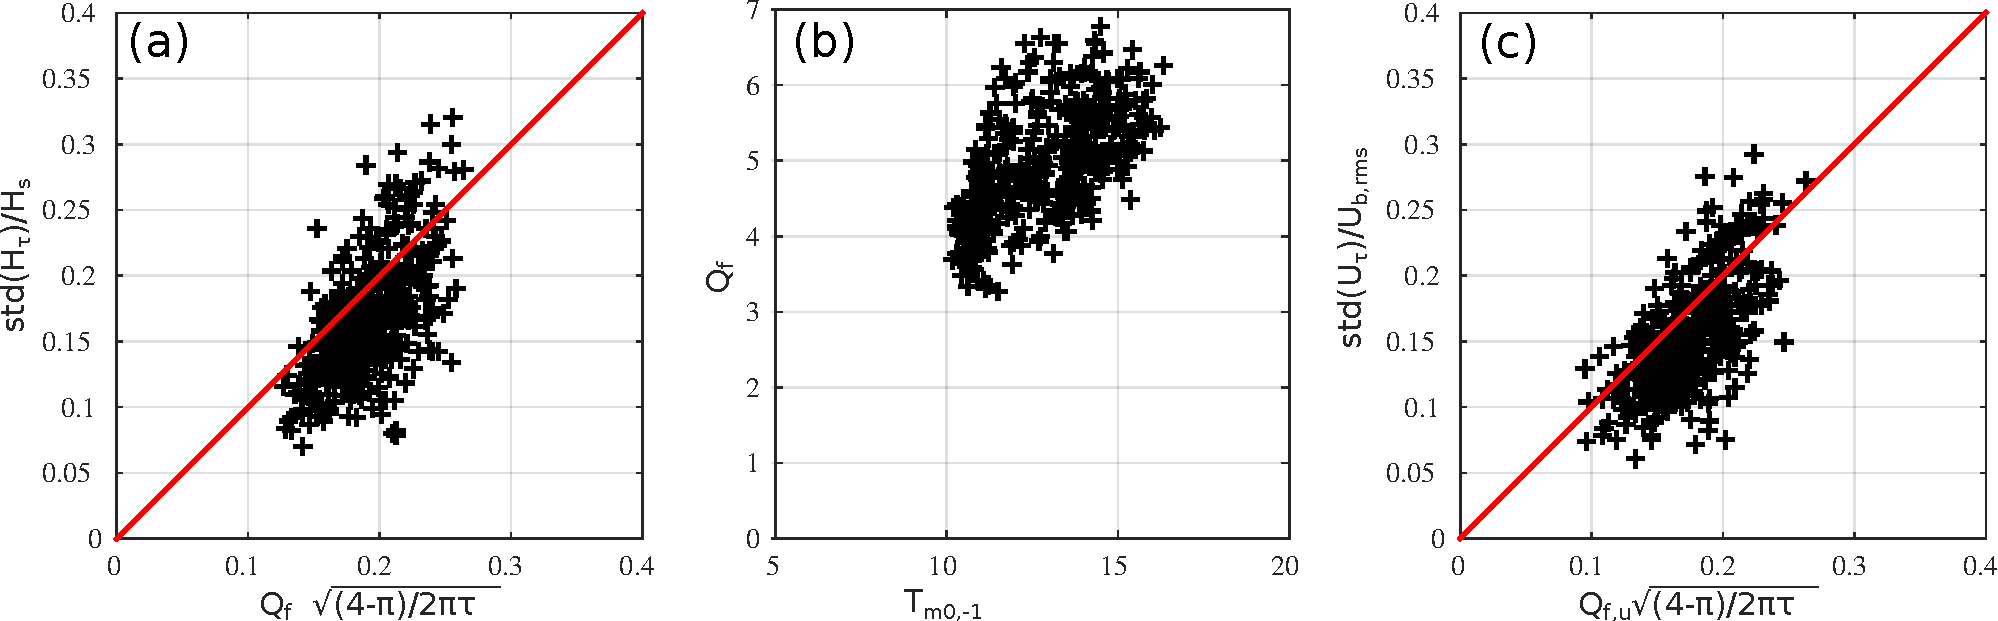
\includegraphics[width=\textwidth]{FIGS_CH_GROUPS/Qf_test.pdf}}
%\vspace{3.64in}
  \caption{Variability of measured parameters over 21 days of measurements in Bertheaume bay, January 2004 using $\tau=180$~s and each symbol corresponds to 1 hour of data: (a) Standard deviation of $H_{\tau}$ normalized by $H_s$ as a function  of the predicted variability using $Q_f$ (b) correlation of $Q_f$ and the mean period $T_{m0,-1}$, (c) variability of bottom orbital velocity amplitude $U_{b,\mathrm{rms}}$ against the relevant $Q_{f,u}$ peakedness parameter.}
\label{fig:groupsQf}
\end{figure}
%%%%%%%%%%%%%%%%%%%%%%%%%%%%%%%%%%%%%%%%%%%%%%%%%%%%%%%
Figure \ref{fig:groupsQf}.a shows that the predicted variability is not exactly like the estimated variability, but it provides a useful order of magnitude, with the "noise" on wave height estimate decreasing like $\sqrt{1/\tau}$, which is why wave records are normally taken over 20 minutes. In the present case, using $2\tau = 20$ minutes averaging instead of averaging over $2\tau = 3$~minutes reduces statistical uncertainties by a factor $\sqrt{20/3}=2.6$, giving a mean value of $\mathrm{std}(H_\tau)/ H_s=6.4\%$, which is of the same order of magnitude as the 5\% relative uncertainty for buoy data for wave heights around 2~m  that is estimated from triple-collocation techniques \citep{Dodet&al.2022}. This suggests that sampling errors caused by wave groups are a large part of the uncertainty in buoy data.

It is always possible to average over longer times but at some point one loses the time resolution that may be needed to investigate how the wave height varies during the tidal cycle or due to other fast evolving phenomena. We also note that quantities that involve higher frequency moments of order $n$ such as the orbital velocity with $n=2$ are less "groupy", their spectrum shape given by $E(f)f^n$ are broader than $E(f)$,  and we can compute a similar $Q_f$ for these parameters that will be lower, as shown in  \ref{fig:groupsQf}.c, using the bottom orbital velocity data from the Nortek Vector instrument. I used pressure and velocity at the ocean bottom in Figure \ref{fig:groupsQf}.a and \ref{fig:groupsQf}.c, and these are already filtered by the water depth, so that the difference between these  $Q_f$  and  $Q_{f,u}$ is not as large as it would be if one used surface elevation and surface velocity.  


\subsection{Spatial maps}
Following the same steps we took for time series, we may imagine that an instrument provides a wave height  $H_{L}$ from a spatial average over a 
square of side $L$ \citep{Lenain&al.2023,Ardhuin&al.2024}. The wave height estimate $H_L$ is  again a $\chi$-distributed random variable with its variance and mean given by  functions of the number of 
degrees of freedom, and their ratio given by eq. (\ref{eq:groups_var_nu}). The only difference is that now  $\nu_{f,H}$ is replaced by 
\begin{equation} 
\nu_{\mathrm{kk},H}=1/ Q_{\mathrm{kk},H}^2 dk_x dk_y \label{eq:nukk}
\end{equation}

 where $dk_x dk_y$ is the spectral resolution of the spectral analysis, corresponding to $dk_x dk_y=(2 \pi)^2/(2 L)^2$, with 
\begin{equation} 
   Q_{\mathrm{kk}}^2 = \frac{  \int_{-\infty}^\infty \int_{-\infty}^\infty E^2(k_x,k_y)\mathrm{d}k_x \mathrm{d}k_y }{\left( \int_{-\infty}^\infty \int_{-\infty}^\infty E(k_x,k_y)\mathrm{d}k_x \mathrm{d}k_y  \right)^2} \label{eq:Qkk},
\end{equation}
where  $E(k_x,k_y)$ is the centrally symmetric double-sided spectrum. If one uses the single-sided spectrum instead, as we did for frequency spectra in eq. (\ref{eq:Qf}), the numerator of eq. (\ref{eq:nukk}) should be 2, as in  eq. (\ref{eq:nuf}). 

This expression is easily verified by taking a wave spectrum $E(k_x,k_y)$, simulating the ocean surface map $\zeta(x,y)$ using random phases, and computing the variance over square tiles of side $L$, as illustrated in Fig. \ref{fig:groups_maps}. The theory, combining eq. (\ref{eq:nukk}) and eq. (\ref{eq:groups_var_nu}) gives 
\begin{equation} 
 \frac{\mathrm{std}(H_L)}{\mathrm{mean}(H_L)} \simeq \pi \sqrt{2}  Q_{\mathrm{kk}} /  L,
   \label{eq:groups_var_2DY}
\end{equation}
which a good approximation in cases where $L$ is much larger than the dominant wavelength. 
%%%%%%%%%%%%%%%%%%%%%%%%%%%%%%%%%%%%%%%%%%%%%%%%%%%%%%%
\begin{figure}[htb]
\centerline{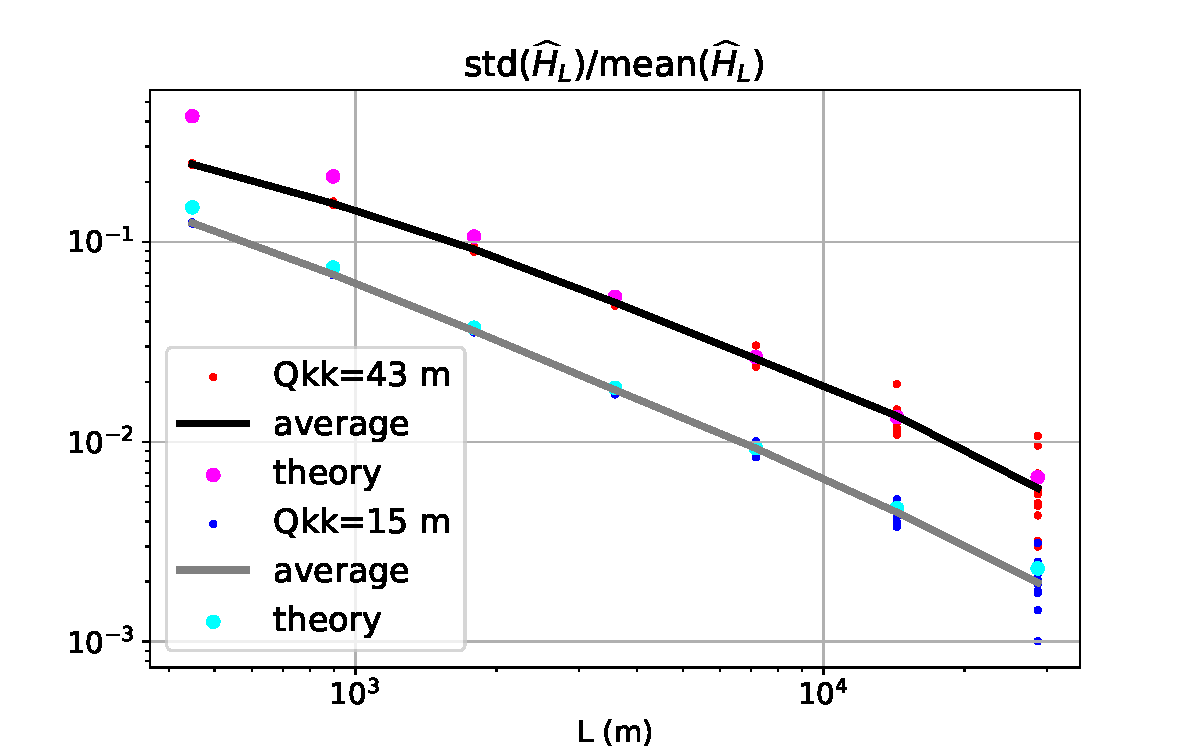
\includegraphics[width=0.9\textwidth]{FIGS_CH_GROUPS/std_maps.pdf}}
%\vspace{3.64in}
  \caption{Variability of $H_L$ in simulated surfaces from 2 different wave spectra, one with $Q_{\mathrm{kk}}=43$~m and the other with $Q_{\mathrm{kk}}=15$~m. These two spectra are shown below in Fig. \ref{figure:groups_storm2}. for each spectrum, 10 surface realisations were generated using random phases, and the average standard deviation is compared to the 
  theoretical value from eq. (\ref{eq:groups_var_2DY}). The notebook that generated this figure is available on \href{https://github.com/ardhuin/waves_in_geosciences/blob/main/NOTEBOOKS/chapter_groups_figure_Qkk_stdH_2D_maps.ipynb}{github}.}
\label{fig:groups_maps}
\end{figure}
%%%%%%%%%%%%%%%%%%%%%%%%%%%%%%%%%%%%%%%%%%%%%%%%%%%%%%%


\subsection{Along-track variability in altimeter data}
A practical important application of the result for spatial maps is the interpretation of the most common measurement of wave heights from space, usinbg satellite altimeters. Looking at data from storm Dennis in the North Atlantic in 2020, as illustrated in Fig. \ref{figure:groups_storm1}, \cite{DeCarlo&al.2023} were surprised to find that for the same mean wave height of 9.3~m, the CFOSAT altimeter beam gave a very small variability on the north side, and a twice larger variability on the south side. What is this variability telling us about the sea state? 
%%%%%%%%%%%%%%%%%%%%%%%%%%%%%%%
\begin{figure}[h!]
\centerline{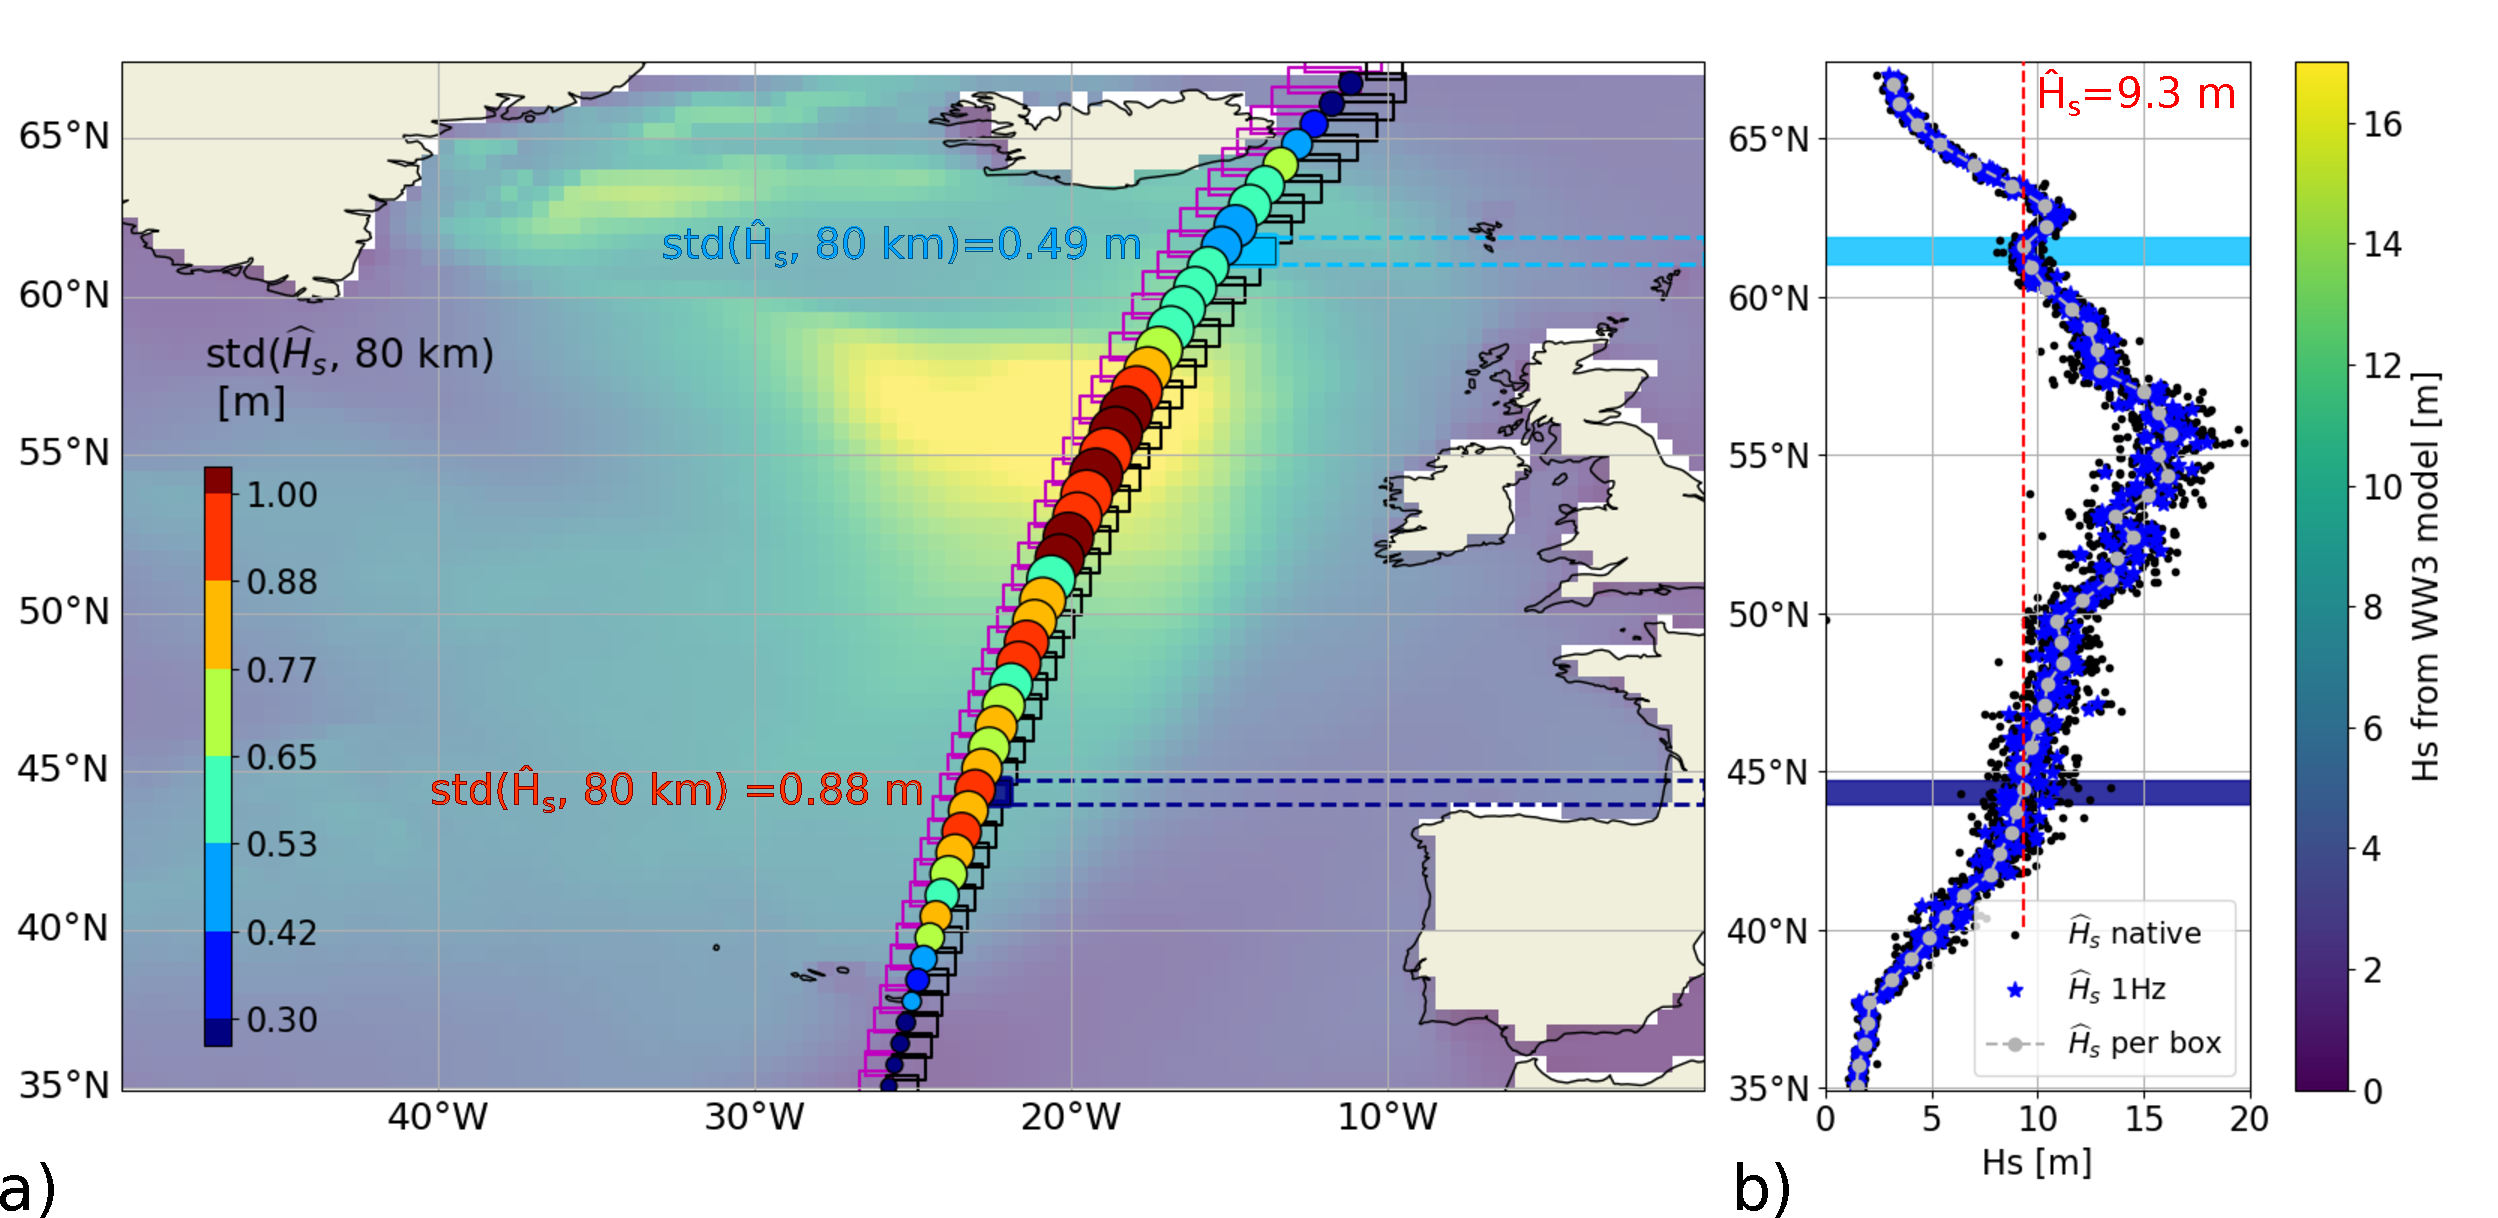
\includegraphics[width=\textwidth]{FIGS_CH_GROUPS/DeCarlo_fig1.pdf}}
    \caption{a) Map of wave heights in the North Atlantic at 09:00 on 14 February 2020, as provided by the model hindcast of \cite{Alday&al.2021}, overlaid with circles located at the center of SWIM box estimates for the L2-CWWIC wave spectra. Circles are sized by the L2-CWWIC $H_s$ estimate and color corresponds to $\mathrm{std}(Hs)$; b) corresponding measured $H_s$ values as a function of latitude (y-axis) : black small dots represent native measurements at 4.5 Hz, blue stars represent the 1~Hz averaged and grey circles represent the $H_s$ averaged over a box. Two boxes are selected for the case study: box A - highlighted in light blue - is at 62$^\circ$N, and box B - in dark blue - is at 44$^\circ$N.} 
   \label{figure:groups_storm1}
\end{figure}
%%%%%%%%%%%%%%%%%%%%%%%%%%%%%%%

The great thing with CFOSAT is that it is the first satellite that combines an altimeter with a wave scatterometer (which provides a measurement of the directional wave spectrum) in the same instrument called SWIM \citep{Hauser&al.2021}. We can thus use the measured wave spectra to understand details in the altimeter data.  In particular we can use the directional spectrum to compute $\Psi$, the spectrum of the envelope. %The maximum value of $H_s$ reported by CFOSAT in the storm was estimated at 17.9~m when using a the average over one measurement cycle (there are 4.5 such measurements per second), or 17.9~m when averaged over 1 s. More interesting to us was, 
Taking the measured wave spectra and simulating the surface and its envelope, as done in Fig. \ref{figure:groups_storm2} makes it easier to visualize the importance of the spectral shape for the defining the spatial variability of wave heights $H_r$. Both panels (c) and (d) correspond to spatially homogeneous sea states with a uniform $H_s$. However, any measurement of waves will be sensitive to the "lumps" of high values and low values that are best seen in the envelope map of Fig. \ref{figure:groups_storm2}.f. The only way to remove this effect of wave groups in the measurements would be to average in time as these groups propagate fast and randomly appear and disappear. 

%%%%%%%%%%%%%%%%%%%%%%%%%%%%%%%
\begin{figure}[hbt!]
\centerline{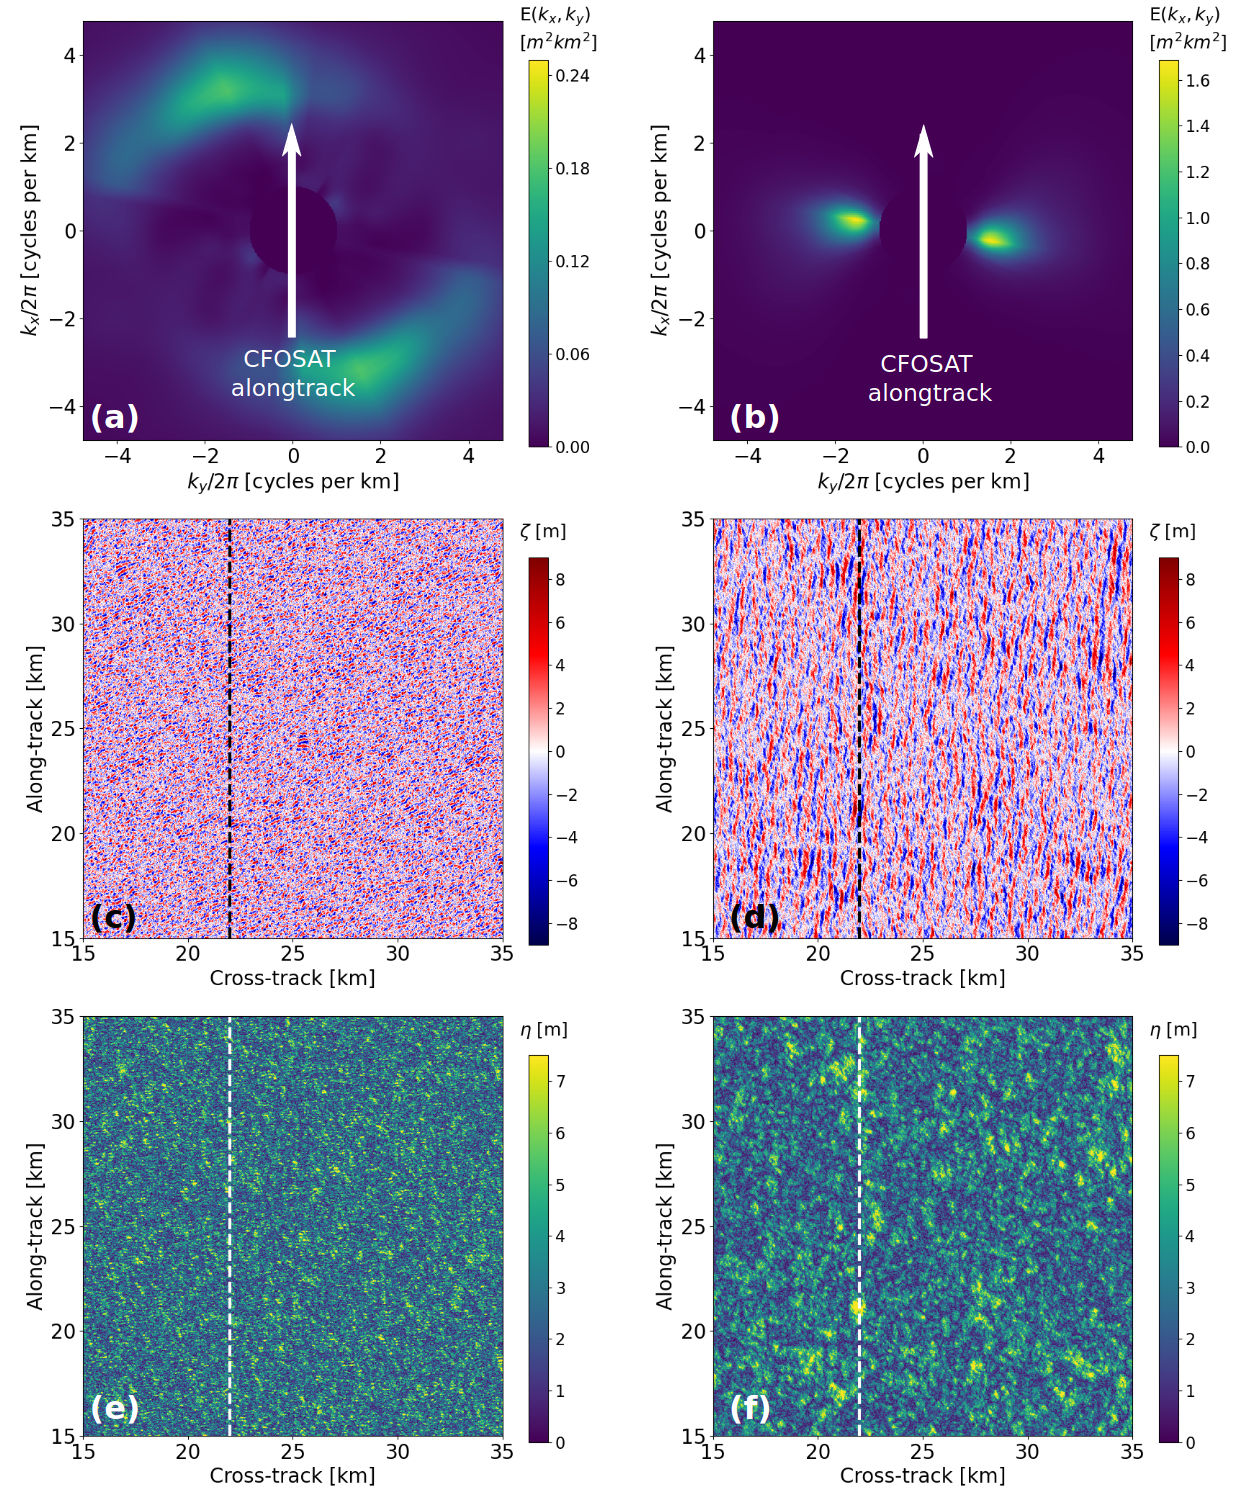
\includegraphics[width=\textwidth]{FIGS_CH_GROUPS/DeCarlo_fig2.jpg}}
    \caption{From wave spectra (top) to surface elevation envelope (bottom): the surface elevations maps in the middle line are simulated using the CFOSAT-derived spectra (these are L2S product corrected to give the same wave height as the nadir beam), with random phases. Combining the real and imaginary parts of the simulated surface gives the envelope. The left column is for a broad wave spectrum with a lower peak period. The right column has the same wave height but a long peak period and narrower spectrum. } 
   \label{figure:groups_storm2}
\end{figure}
%%%%%%%%%%%%%%%%%%%%%%%%%%%%%%%


Although the details will be given only in the next chapter, we may guess that an altimeter samples the ocean with some filtering function that not a square boxcar but some sort of disc of radius $r$, and  we can imagine that the local height is some convolution of the envelope
\begin{equation}
    H_{r}(x,y) = 4\sqrt{\frac{2}{\pi}} (\eta \otimes g_{r})(x,y).
   \label{eq:relation_Hs_eta}
\end{equation}
In practice a single altimeter gives estimates along a single track in the $(x,y)$ plane and the filter function $g_r$ can be a little complicated. For Delay-only altimeters the detailed form of $g_r$ was derived in \cite{DeCarlo&al.2023}, and for our purpose a good approximation is a Gaussian filter of radius $r_a=r_C/4.5$, giving a filter $G_{r_a}=\exp{(-k^2 r_a^2)}$ for the power spectrum in Fourier space, with $r_C$ given by \cite{Chelton&al.1989} as the radius of the region of the ocean surface that may contribute to the measured signal (again, details will follow in the next chapter), 
\begin{equation}
    r_C =\sqrt{\frac{ 2 h_o H_s+ 2 \delta_R}{1+h_o/R_E}} \label{eq:rC}
\end{equation}
where $h_o$ is the satellite orbit height above the ocean, $R_E$ is the Earth radius and $\delta_R$ is the range resolution of the altimeter.  
 
 
Using the double-sided wave spectrum $E(k_x,k_y)$ of the surface elevation, defined for $(k_x,k_y)$ in the entire wavenumber plane and centrally symmetric, the region of the envelope spectrum for $k \ll k_p$, with $k_p$ the wavenumber peak, is 
proportional to
\begin{equation}
    \Psi_{2}(k_x,k_y) = 8 \int_{-\infty}^\infty 
    \int_{-\infty}^\infty
E(u,v)E(u+k_x,v+k_y)\mathrm{d}u \mathrm{d}v,
\end{equation}
in which $\Psi_{2}$ is also double-sided. From  eq.~(\ref{eq:relation_Hs_eta}), the spectrum of $H_r$ is
\begin{eqnarray}
\Psi_{H_r}(k_x,k_y) &= & \frac{32}{\pi}  \Psi(k)  G_{r}(k_x,k_y) =  \underbrace{\frac{32}{\pi} \frac{8 - 2\pi}{H_s^2}   \Psi_2(k_x,k_y)}_{\Psi_{H_0}(k_x,k_y)}  G_{r}(k_x,k_y)\label{eq:eq2_inFourier}
\end{eqnarray}
with $H_s$ the usual significant wave height and $G_{r}=G_{r_a}$ when considering a single altimeter measurement.

We will now average data along the track, at least over 0.05~s corresponding to the 20~Hz rawest data downlinked for most instruments, and corresponding to 350~m distance along the track. For delay-only measurements, these data are fairly noisy and most users typically use at least 1~Hz data (averaged over 7~km) or longer time averages. For simplicity we take the satellite track along the $x$-axis, and we consider an averaging length $d_1$. 
Integrating $\Psi$ for $k_x > k_1$, amounts to integrating $\Psi_{H_r}(k_x,k_y)$ to get the expected variance up to the  cut-off wavenumber along $k_x$, $k_1\simeq \pi / d_1 $, giving $\mathrm{var}(H_{r},d_1)$, the group-induced fluctuations of $\widehat{H}_s$ 
\begin{equation}
\mathrm{var}(H_{r}, d_1) = \int_{-\infty}^{\infty} \int_{k_x > |k_1| } \Psi_{H_0}(k_x,k_y)  G_{r}(k_x,k_y) \mathrm{d}k_x \mathrm{d}k_y. \label{eq:varfromspec2D}
\end{equation}
% pi/2 * (2/ra^2 - 4 k1 / sqrt(pi) ra) = pi * ka^2 - 2 ka*2k1  ka = 
Here again, if the filter $G_{r}$ is zero outside of a very small range of wavenumbers, we can approximate $\Psi_{H_0}(k_x,k_y) \simeq \Psi_{H_0}(k_x=0,k_y=0)$ and take this value out of the integral, and the integral is related to the effective area of the filter in the wavenumber plane which we approximate as a disk of radius $1/r_a$, with an area $\pi /r_a^2$, given by the integral of $G_{r}$ over the entire wavenumber plane, and we remove a band of width $2 k_1$ and length $2/r_a$ because we are only averaging over $d_1$ so that wavelengths longer than $2 d_1$ cannot contribute to our signal and must be excluded. This gives,  
\begin{eqnarray}
    \mathrm{var}(H_{r},d_1) &\simeq&  \Psi_{H_0}(0,0)   \int_{-\infty}^{\infty} \int_{k_x > |k_1| } G_{r}(k_x,k_y) \mathrm{d}k_x \mathrm{d}k_y \nonumber \\
    &\simeq&  \Psi_{H_0}(0,0)  \pi\left(1 / {r_a}^2 - 4 k_1/ r_a \right) \nonumber\\
    &\simeq&  \frac{32}{\pi} \frac{8 - 2\pi}{H_s^2}   \Psi_2(0,0)   \pi  \left(1 / {r_a}^2 - 4 k_1/ r_a \right) \nonumber\\
    &\simeq&   Q_{kk}^2 H_s^2(8 - 2 \pi) \left(1 / {r_a}^2 - 4 k_1/ r_a \right)  , 
\end{eqnarray}
where we have defined 
a two-dimensional spectral peakedness $Q_{kk}$ which is measured in meters,
\begin{equation}
    Q_{kk}^2 = \frac{\iint_{} E^2(k_x,k_y)\mathrm{d}k_x\mathrm{d}k_y}{\left(\iint_{}E(k_x,k_y) \mathrm{d}k_x\mathrm{d}k_y\right)^2} = \frac{32 \Psi_2(k_x=0,k_y=0)}{H_s^4}.
\label{eq:bandwith_2D}
\end{equation}


This expression gives the approximate value for the standard deviation,
\begin{equation}
    \mathrm{std}(H_{r},d_1) \simeq  H_s   Q_{kk}  \sqrt{ (4-\pi) \left[2/r_a^2 -  8 k_1 / r_a\right] }.\label{eq:std_Hs_from_Qkk}
\end{equation}

{This variability of $H_{r_a}$, which we have defined as the contribution of wave groups to the variability of "measured" wave heights $\widehat{H}_s$ is thus the product of three factors: the significant wave height $H_s$, the shape of the wave spectrum as quantified by $Q_{kk}$, and the effective range of spatial scales over which the variance is integrated. That last factor is a function of the smoothing effect of the altimeter, represented by the filtering scale $r_a$, and the distance $d_1=2\pi / k_1$ over which  we consider the variability.


%%%%%%%%%%%%%%%%%%%%%%%%%%%%%%%
\begin{figure}[ht!]
\centerline{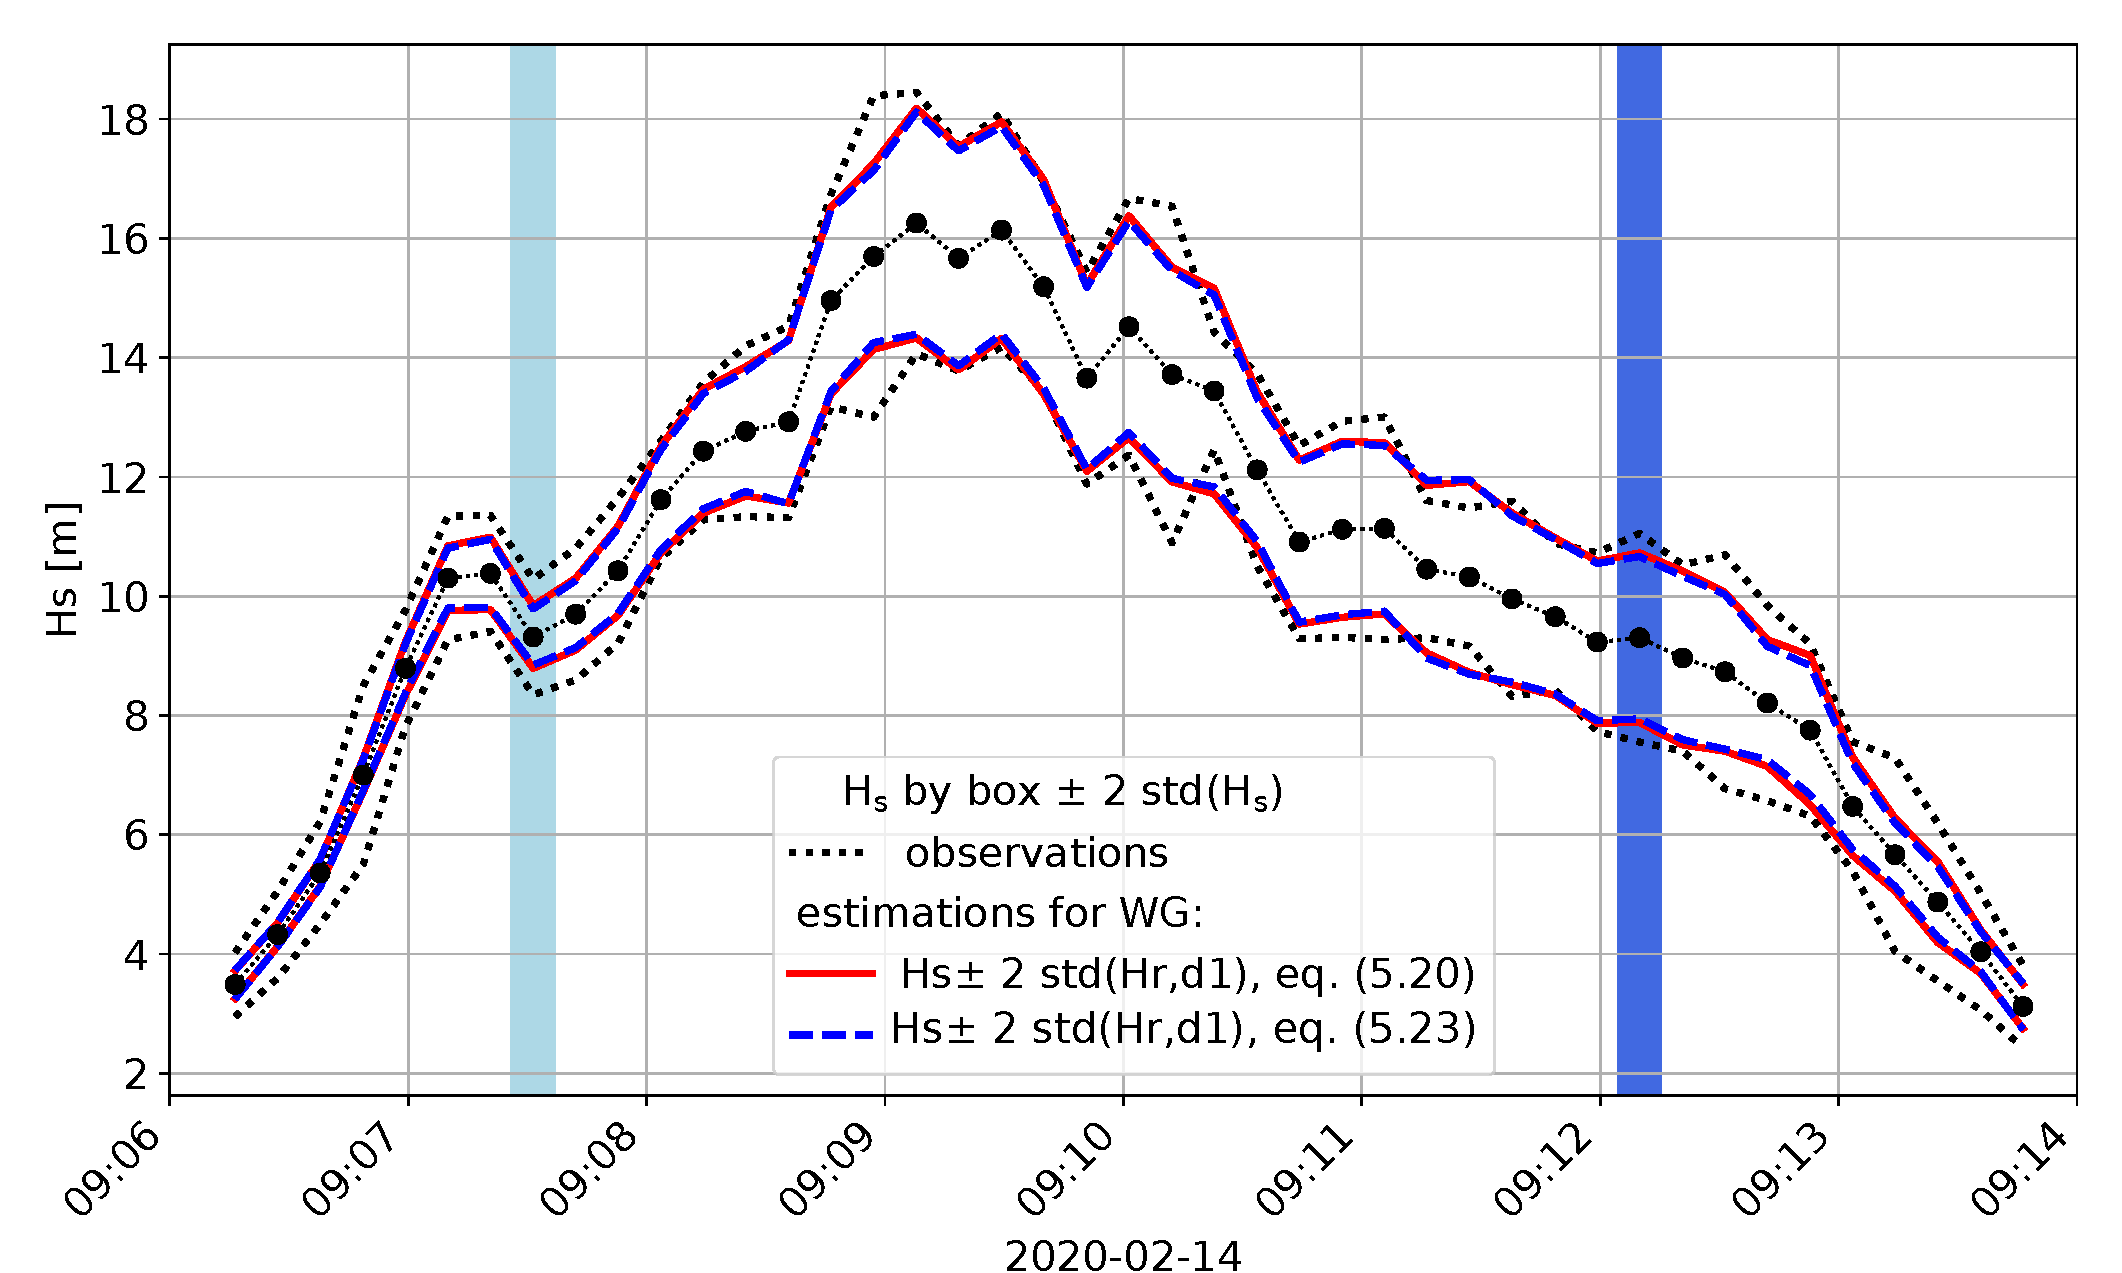
\includegraphics[width=0.75\textwidth]{FIGS_CH_GROUPS/groups_Storm_Dennis_2023_fig3.pdf}}
    \caption{Values of measured $H_s$, averaged over 80~km - black circles - ,  and corresponding $\mathrm{std}(Hs)$ - black dash-dotted lines - in the satellite data, for the CFOSAT track shown in Fig.~\ref{figure:groups_storm1}. Estimations of $\mathrm{std}(H_r,d_1)$ are also represented - in red and blue.} 
   \label{figure:groups_storm3}
\end{figure}
%%%%%%%%%%%%%%%%%%%%%%%%%%%%%%%
We can use our theory to verify that in the case of narrow spectra, the expected effect of wave groups gives a standard deviatin of the estimates of wave heights $H_r$ that is similar to the standard deviation of the measurement over a 80~km segment along the satellite track (Fig. \ref{figure:groups_storm3}). 

On the contrary, for the broader wave spectrum, the effect of wave groups is much smaller than in the measurements: it is possible that the data contains true gradients of the underlying $H_s$, and we also know that measurement noise (known as speckle) is often the dominant source of variability in the measured values. This is one of the main reason for the development of Delay-Doppler altimetry which has a much lower level of speckle noise due to the averaging of different indepedent Doppler "looks" for the same measurement. 

Using eq. (\ref{eq:std_Hs_from_Qkk}) we can remove the expected contribution of groups and study the influence on other factors on the variability of $H_s$. Figure \ref{fig:groups_global1}, shows that the relative fluctuations in significant wave height is clearly associated with regions of strong mesoscale currents, as we will see in chapter \ref{ch_current}. However, in order to be able to transpose these results to other satellites, we now have to go back to these assumptions about how altimeters actually work, and do a little bit of theory about these instruments and what they actually measure: nadir altimeter do not measure wave height or sea level, they measure waveforms from which wave height and sea level are estimated. 


%%%%%%%%%%%%%%%%%%%%%%%%%%%%%%%
\begin{figure} [ht!]
   \centerline{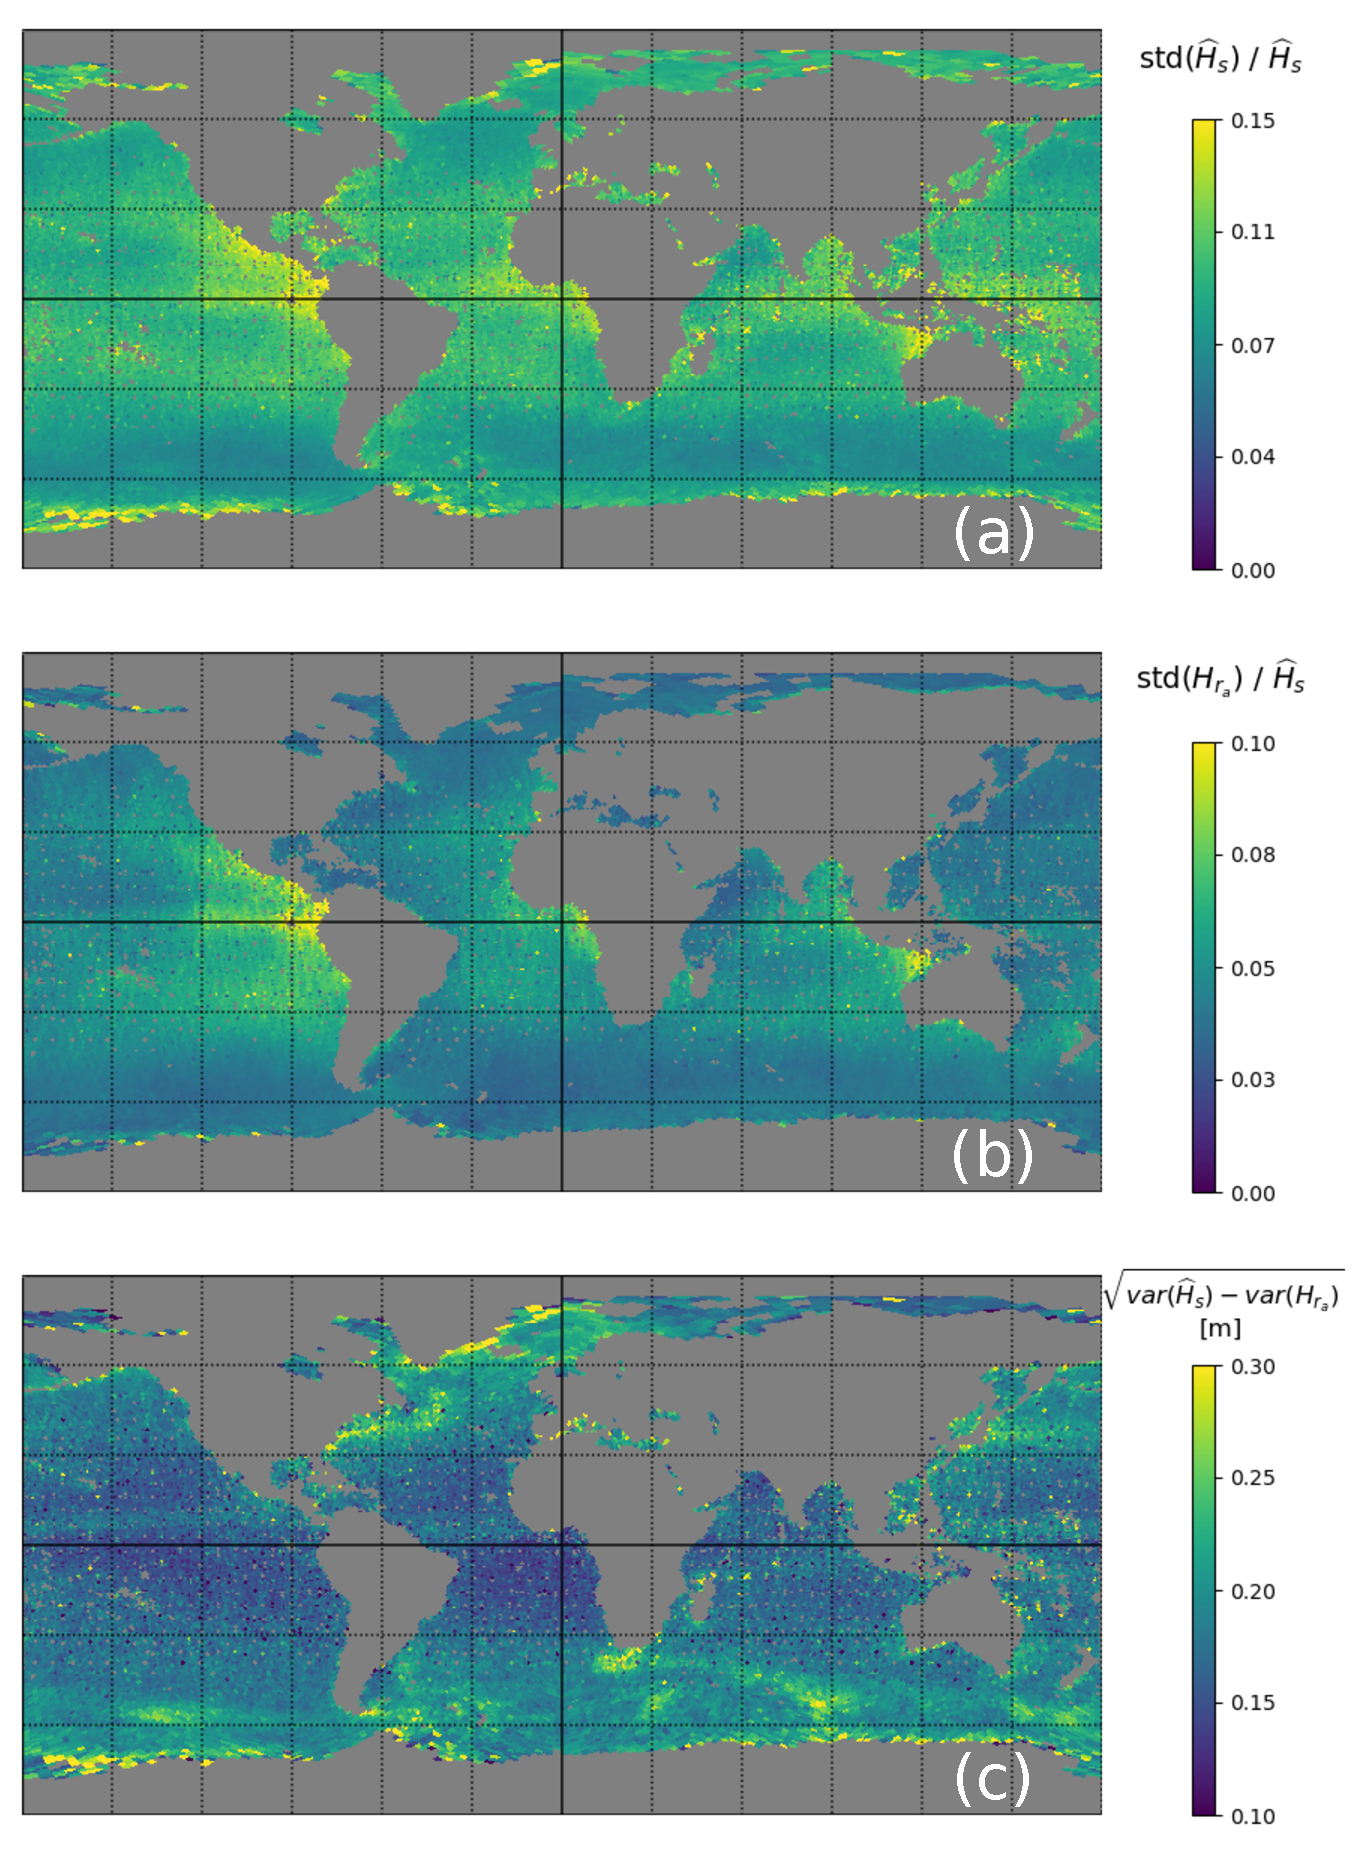
\includegraphics[width=\linewidth]{FIGS_CH_GROUPS/Fig8_map_stdHs_byHs_nadir_vs_L2S.pdf}}
    \caption{Map of the average of a) $\mathrm{std}(\widehat{H}_s)/\mathrm{mean}(\widehat{H}_s)$ - upper panel -, b) $\mathrm{std}(H_s)_\mathrm{{wg}}/\mathrm{mean}(H_s)$ -middle panel - and c) residual standard deviation of $H_s$, in meters, after removing the effect expected
from wave groups - lower panel -, for the years 2020 and 2021 for all the SWIM L2-IWWOC boxes with a $H_s$ above 1.5 m. With the wave group contribution $\mathrm{std}(H_s)_\mathrm{{wg}}$ estimated from SWIM L2S spectra.  reproduced from \cite{DeCarlo&al.2023}.} 
   \label{fig:groups_global1}
\end{figure}
%%%%%%%%%%%%%%%%%%%%%%%%%%%%%%%



\cleardoublepage
\chapter{Wave data from satellites: Skylab (1975) to SWOT (2025)}\label{ch_sat}

It is not possible to cover in a single chapter all the technical development in radar instruments and their processing over the last 50 years. We will thus focus mostly on nadir radar altimeters with some discussion of complementary measurements from Synthetic Aperture Radar (SAR) and wave spectrometer systems. Hopefully more chapters will pop up in Part 3 to go beyond 
this presentation. 

\section{General considerations about radar remote sensing}
Since the invention of radar, the sea was found to be an important source of echoes, at all radar frequencies (from decametric to micro waves). 
This is due to the dielectric properties of sea water. An active radar measures the electromagnetic power received by its antenna. Using the radar equation, this power (in Watts)
is normalized by the antenna-target distance, the antenna size, and the emitted power. This gives the normalized radar cross section (NRCS), a quantity without dimensions that is often represented 
by the symbol $\sigma_0$. 
$\sigma_0$ depends on the surface geometry but it also varies with the radar frequency and polarization,  and observation direction (azimuth and incidence angles). %In particular, $\sigma_0$ highly depends on the radar wavelength and of the wave radar incidence angle relative to the surface.
The phase properties of the signal can also be used to estimate velocities at the ocean surface: current and wave orbital velocities \citep{Nouguier&al.2018,Rodriguez2018}. 

%A down-looking (nadir) radar will measure a high $\sigma_0$ for a smooth sea surface. If waves are present, the surface echoes may be considered as the incoherent superposition of the facet echoes. 
%%%%%%%%%%%%% figure
\begin{figure}[htb]
\centerline{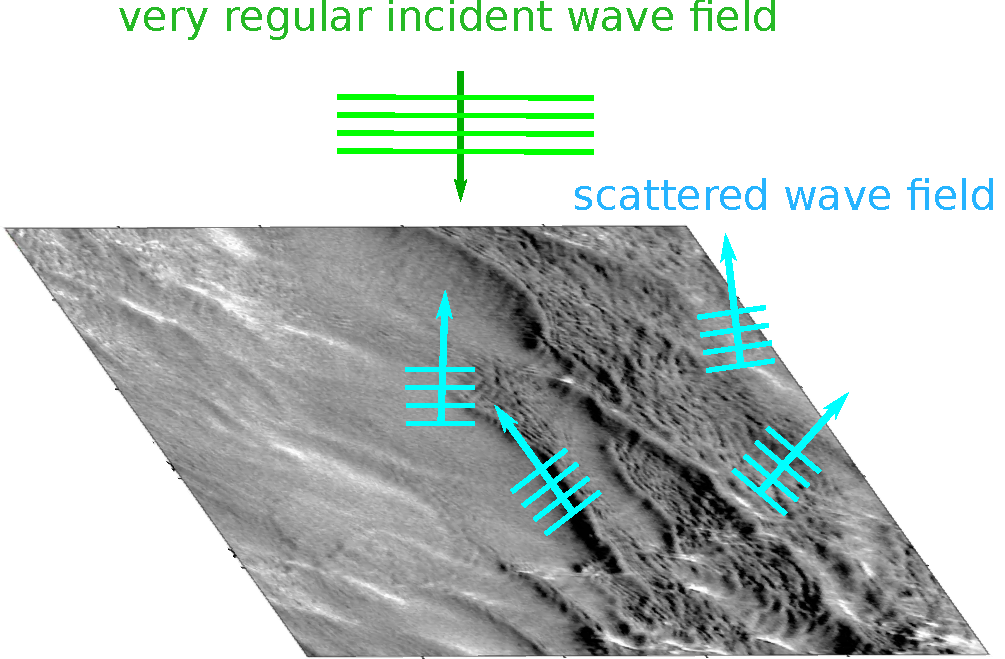
\includegraphics[width=0.7\textwidth]{FIGS_CH_SAT/scatter.pdf}}
%\vspace{3.64in}
  \caption{Conceptual schematic of microwave radar waves scattering at the sea surface. The grey shades are an example of a map of surface slopes estimated from a polarimetric system and covering a region of about 1 by 1 meter \citep{Laxague&al.2018}.}\label{fig:scatter}
\end{figure}
%%%%%%%%%%%%% end of figure
Now, before we look at radar power of phase, one should realize a few important facts 
\begin{itemize}
\item within the radar field of view, the echoes recieved by the radar are coming from only a very small fraction of the surface: where the ocean is smooth (at the scale of the radar wavelength) only those pieces of the ocean surface that are facing the radar will contribute to the measured reflected signal, where the surface is curved, there will be a very weak scattering in all directions. 
\item the many sources of the echoes on the sea surface have randomly distributed distances (and velocities) relative to the radar, so that  the relative phase of all the echoes is randomly distributed and the sum of the electric fields from all these random sources will have highly fluctuating amplitudes within a few milliseconds as the ocean surface moves: this effect is called "Rayleigh fading" and it introduces speckle noise in the radar measurements. This is very similar to the presence of wave groups in narrow-banded wave spectra. 
\end{itemize}


%\subsection{Satellite radar altimeters}
The choice of the radar frequency is dictated by 
a number of considerations, including atmospheric absorption -- we want to be able to measure a returning echo from the sea surface -- and the 
size of the antenna -- low frequencies give large wavelength that require a proportionally large antenna to have a narrow beam. The radar wavelength 
and frequency are related by the speed of light $c$, namely $f_r = c / \lambda_r$. Different frequency bands have been reserved for Earth remote sensing, although they can be contaminated by military radars and other 
systems. Note that telecommunication systems (FM radio, TV channels, GSM networks, GPS/Galileo positionning systems ...) use different bands  also in the microwave range, and remote sensing may use these 
sources of opportunity for signals that reflect off the sea surface  \citep[e.g.][]{Lowe&al.2002}.


%%%%%%%%%%%%%%%%%%%%%%%%%%%%%%%%%%%%%%%%%%%%%%%%%%%%%%%%%%%%%%%%%%%%%%%%%%%%
\begin{table}[hb]
  \centering
  \begin{tabular}{|c|c|c|c| c |}
 \hline
band name & frequency & wavelenghth & example instrument & satellite  carrying the instrument  \\
 \hline
W  & 94 GHz  & 0.3 cm & CPR & Cloudsat  \\
Ka & 30 GHz  & 0.8 cm & AltiKa or KaRIN & SARAL or SWOT  \\
Ku & 15 GHz  & 2.2 cm & Poseidon 3 & Jason 3  \\
X &  9.6 GHz & 3.1 cm & & TerraSAR-X  \\
C & 6 GHz   & 5 cm & Poseidon 3 or ASCAT & Jason 3 or MetOp \\
S & 3 GHz   & 12 cm & S-SAR &  NISAR \\
L & 1.5 GHz  & 24 cm & SMAP  & SMAP \\
P & 435 MHz  & 70 cm & P-SAR & Biomass (launch  in 2024 or 2025) \\
\hline
\end{tabular}
\caption{Typical average frequencies and wavelengths used for ocean remote sensing in the different radar microwave bands. The actual frequency usually varies during a radar pulse with a bandwidth $B$ that defines 
the range resolution of the instrument. \label{table_radars}}
\label{table_bands}
\end{table}
%%%%%%%%%%%%%%%%%%%%%%%%%%%%%%%%%%%%%%%%%%%%%%%%%%%%%%%%%%%%%%%%%%%%%%%%%%%%

Ocean waves have been monitored from space continuously since the lauch of ERS-1 using altimeters and SARs, as summarized in figure \ref{fig:satellite}
%%%%%%%%%%%%% figure
\begin{figure}[htb]
\centerline{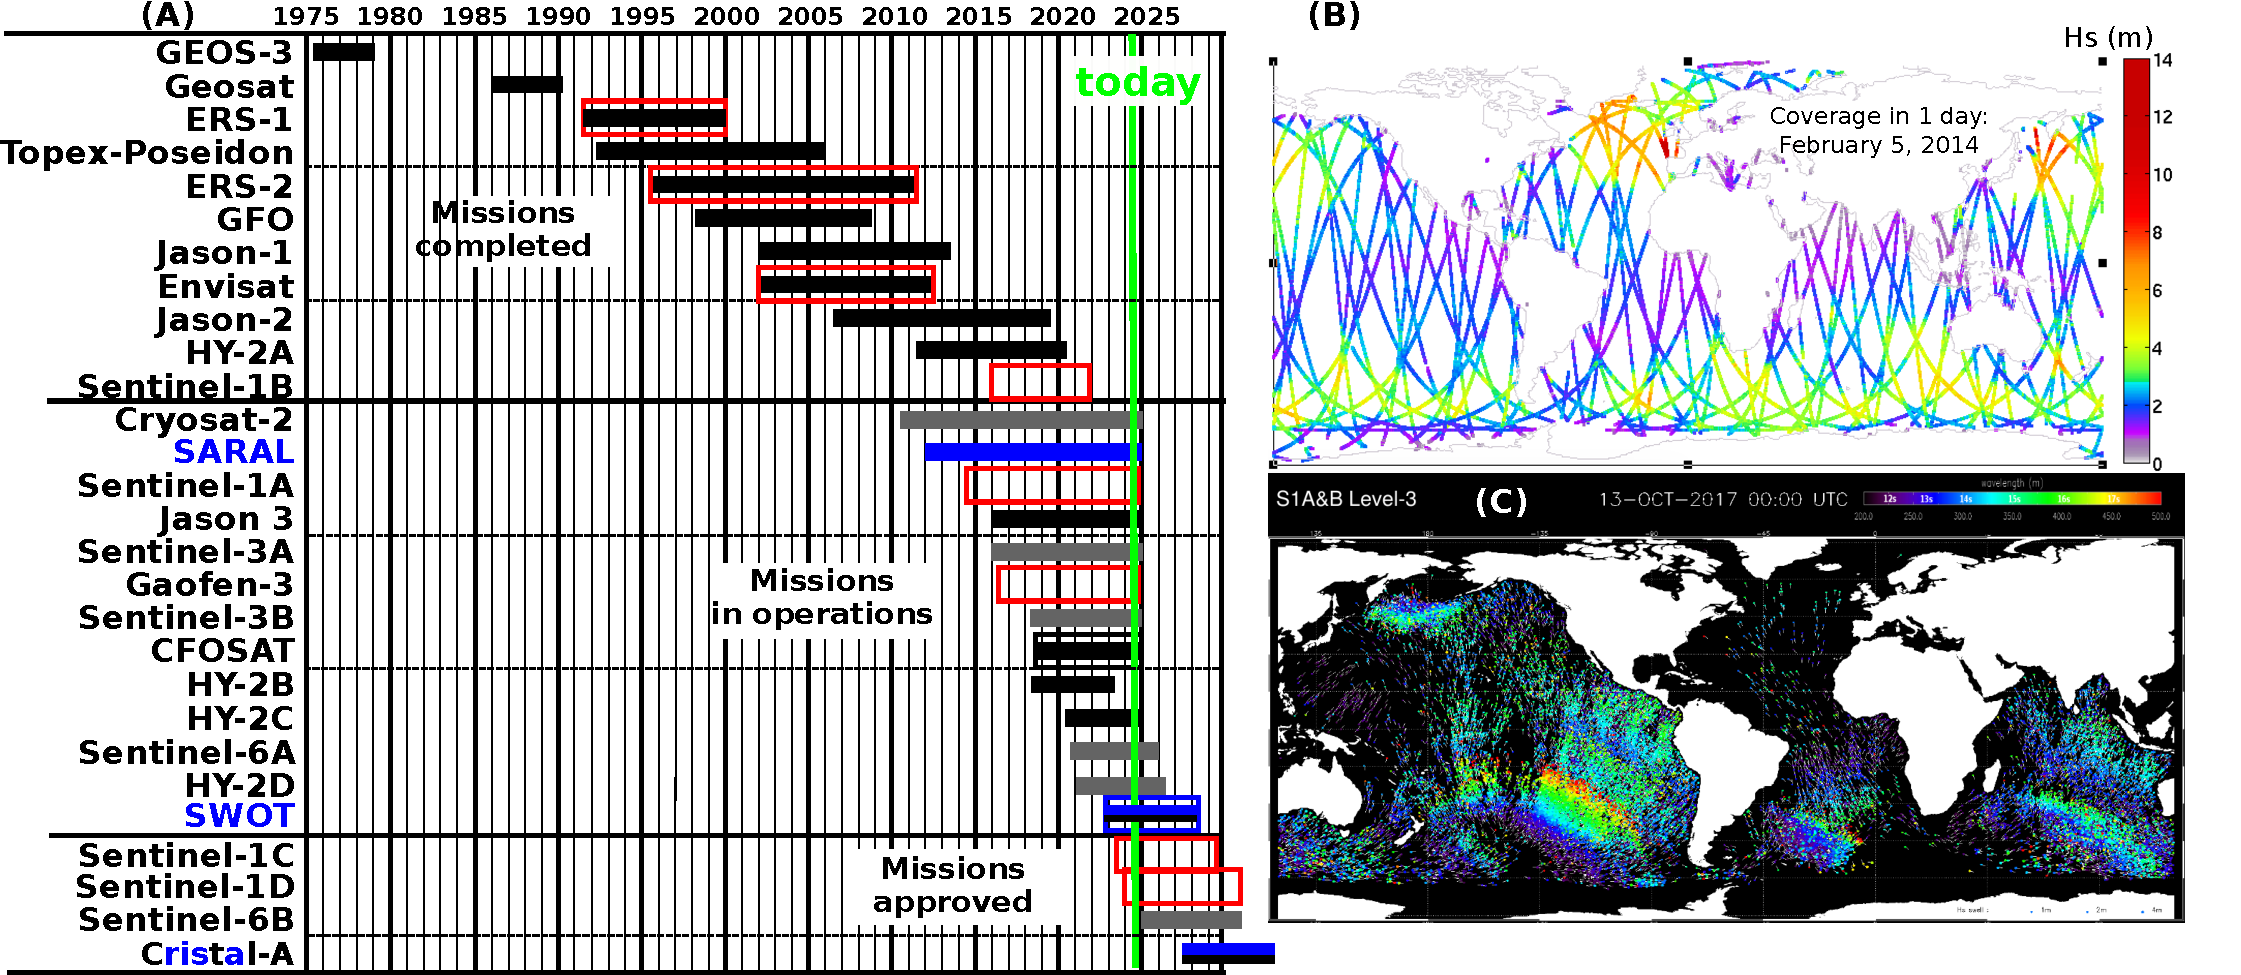
\includegraphics[width=\textwidth]{FIGS_CH_SAT/missions.pdf}}
%\vspace{3.64in}
  \caption{Satellite missions with sea state monitoring objectives.}
    {Time coverage of satellite missions from 1985 to 2030, including nadir and near-nadir altimeters (solid bars), and missions monitoring ocean wave spectra (open boxes) using C-band Synthetic Aperture Radars (red), and real aperture radars in Ku-band (black) or Ka-band (blue). The lighter color (grey and blue) bars correspond to altimeters using Delay-Doppler processing. Source: CEOS database
    \url{http://database.eohandbook.com/}). (B) example of 1-day coverage for Hs measurements with 4 satellite altimeters 
    (C) snapshot of a 'fireworks' plot, the showing the height (size of symbols) peak periods (colors), and directions (barbs) of 
    swell partitions derived from Sentinel-1A and Sentinel-1B wave mode data. Such plots are produced routinely by CMEMS.}\label{fig:satellite}
\end{figure}
%%%%%%%%%%%%% end of figure

\section{Radar altimeters and the The Brown-Hayes model: echoes from a spatially uniform ocean}
Radar altimeter data are, the source of measurements of $H_s$  available at global scale and used for operational wave forecasting
through data assimilation. Contrary to other observation systems, $H_s$ is directly estimated, without the use of a spectral analysis. The usual 
arrangement is a radar antenna looking straight down - at the nadir - on the the sea surface. 

\subsection{Conventional or `delay' altimetry}\label{delay}
%%%%%%%%%%%%% figure
\begin{figure}[htb]
\centerline{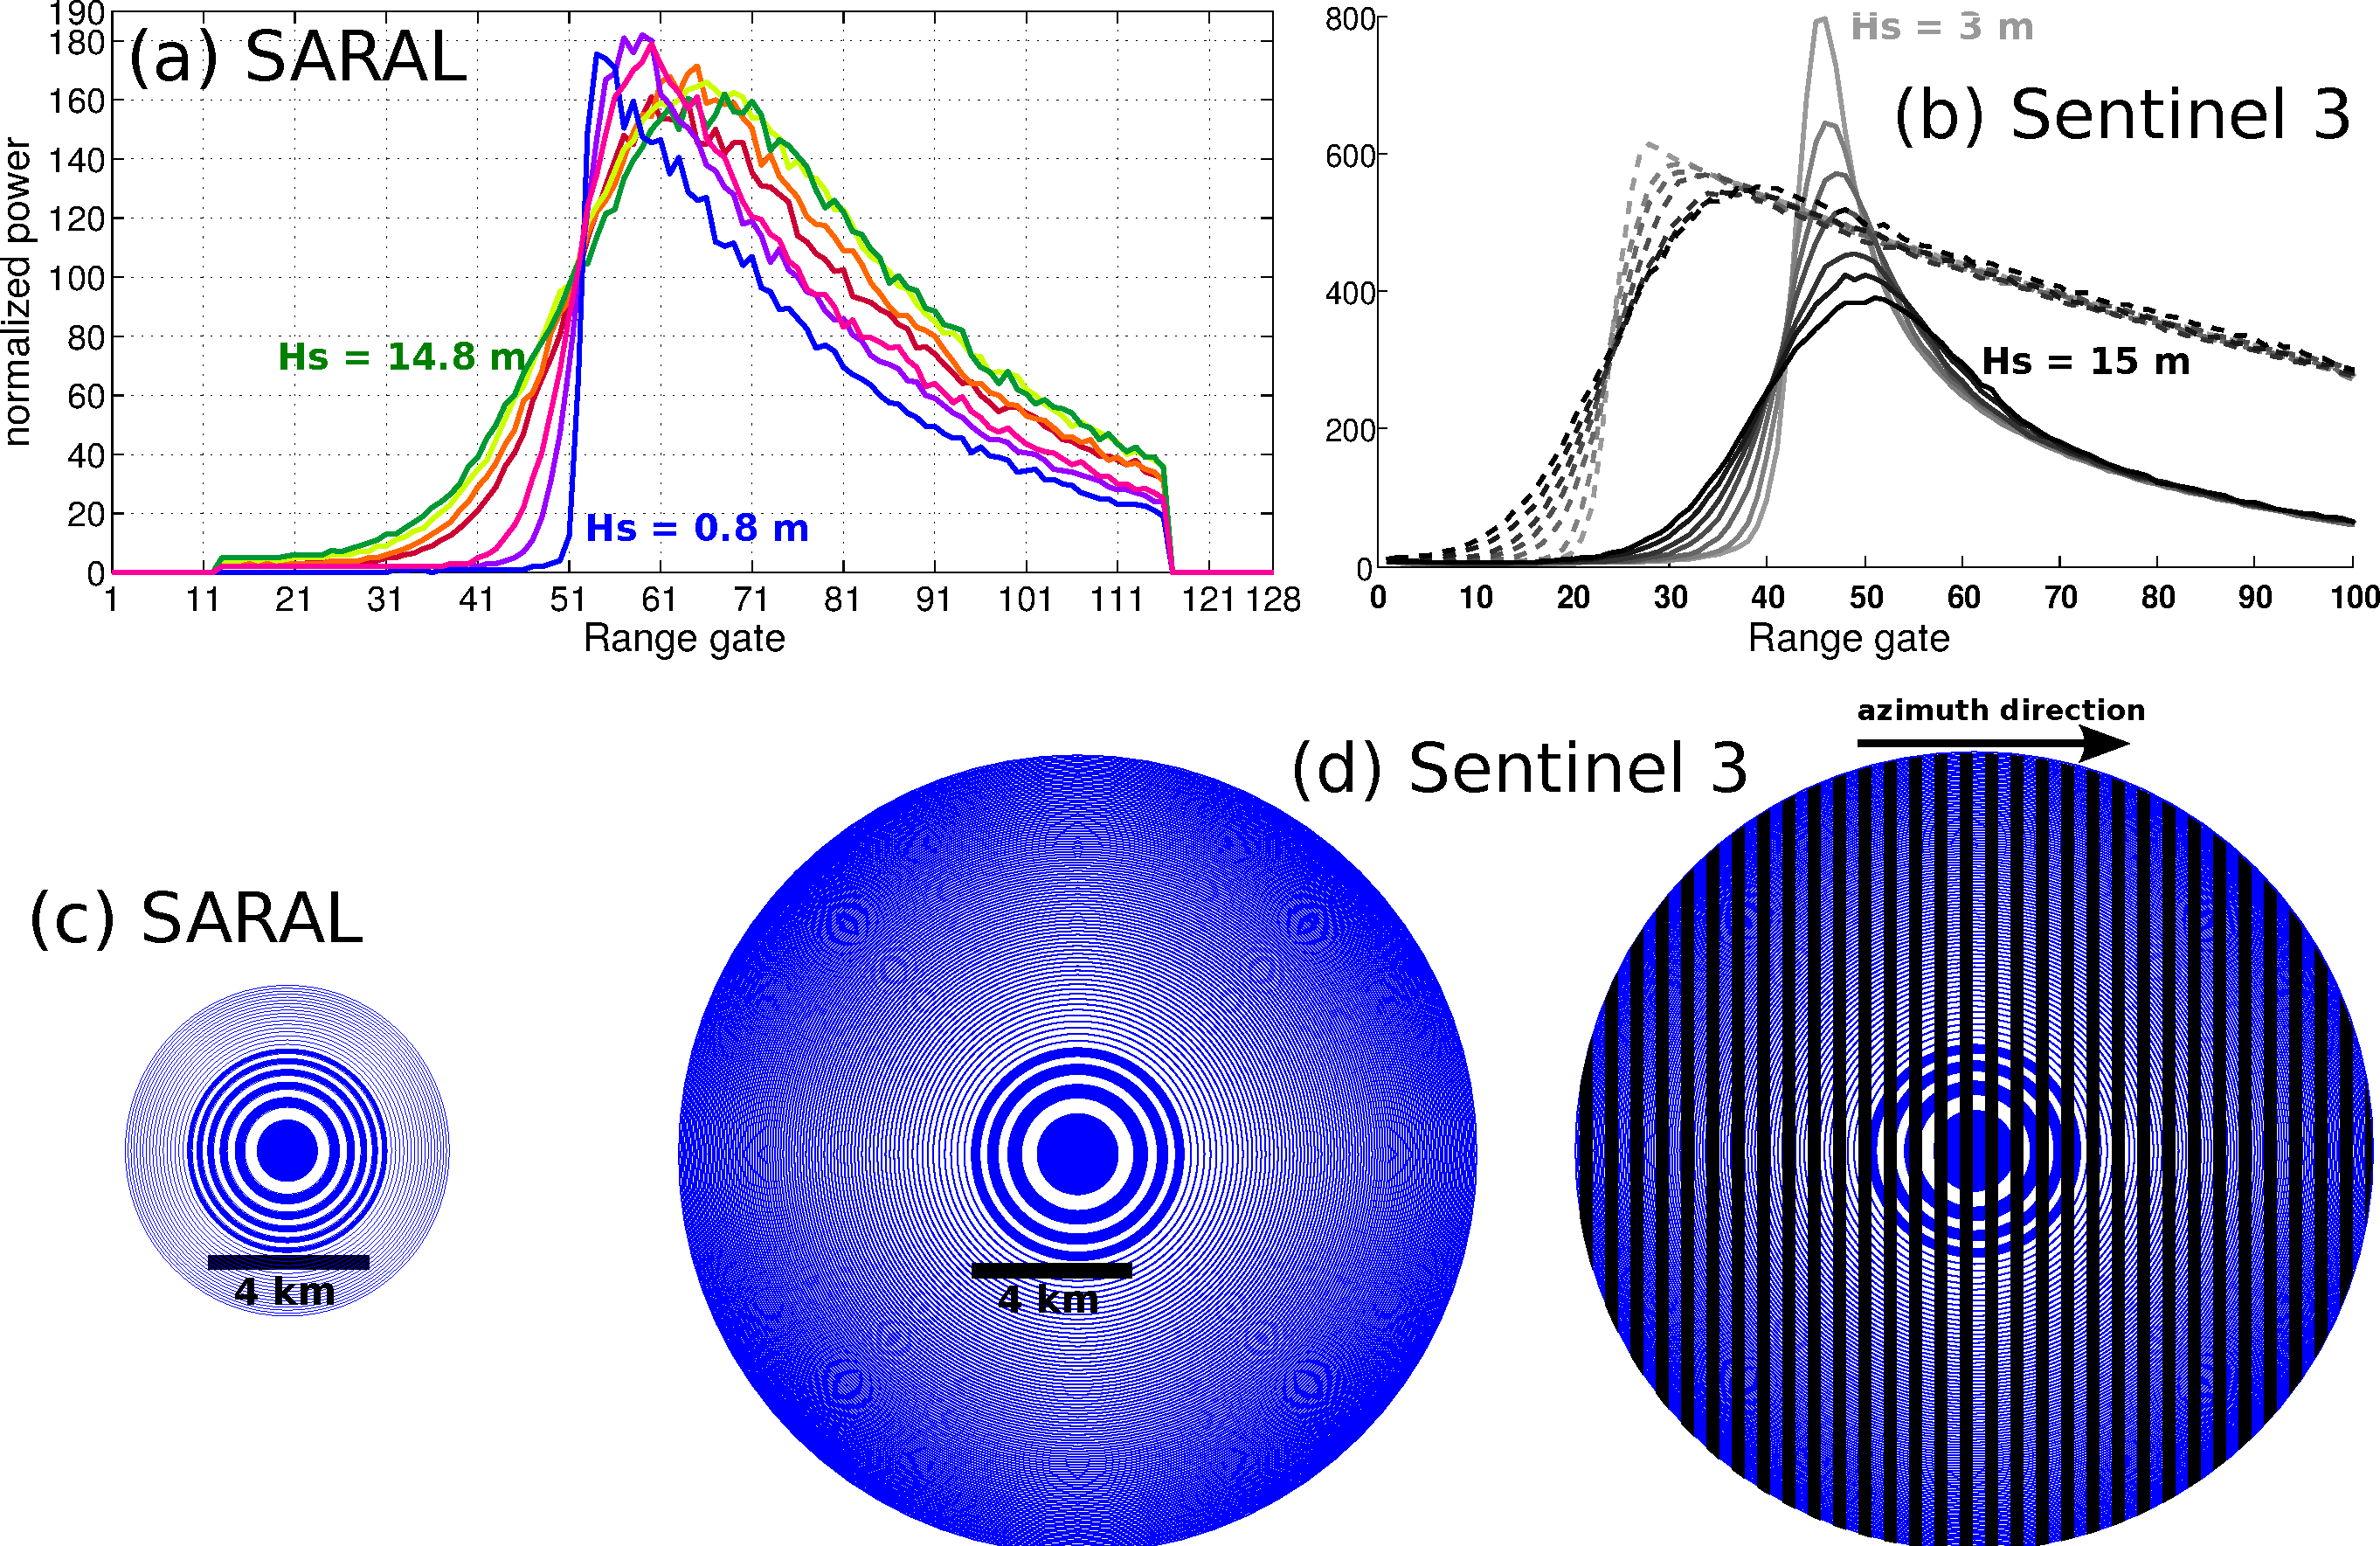
\includegraphics[width=0.9\textwidth]{FIGS_CH_SAT/dessin_footprint.pdf}}
%\vspace{3.64in}
  \caption{Altimeter waveforms and footprints}
    {Example of altimeter waveforms for different wave heights.}
    {(a) These waveforms were selected along the ascending track of SARAL/AltiKa on February 5, 2014, 
    beteen 05:29:49 and 06:20:07 UTC. Each waveform shows the the power measured by the radar as a function of time: 
    time is discretized with intervals of $2 \times 10^{-9}$~s corresponding to 
30~cm range intervals usually called `range gates'. The corresponding wave heights are 0.8, 3.2, 4.6, 9.7, 10.7, 13.2, and 14.8 m. 
Data is available from CNES/Aviso ftp. Each waveform shown here was obtained for 1~s of data, 
 as the median of 40 conscutive waveforms. (b) Similar waveforms from Sentinel 3 using delay-only (dashed) and delay-doppler (solid) for Hs = 3,5,7,9,11,13
and 15 m, for cycle 23 orbit 349, on 25 October 2017 in the Pacific. (c) Spatial coverage of footprints corresponding to the 3-dB antenna lobe pattern, for an 
unrealistic flat sea surface with a uniform roughness, with the first 11 range gates painted alternatively blue and white, 
starting from center. (d) Footprint for Sentinel 3, with the 7 seven range gates colored blue and white, with the azimuth resolution of the Doppler processing indicated by the grey stripes.
} \label{waveform}
\end{figure}
%%%%%%%%%%%%% end of figure
The first main principle of the analysis of the radar echoes is the determination  of the distance, usually called range, based on 
the delay of a radar pulse 
to travel from the transmitting antenna to the target and back to the receiving antenna. Usually the two antennas are the same piece of hardware 
and this is called a `monostatic system'. Because the radar pulse has a finite duration which limits the resolution of the time measurement, 
it is customary to use a varying transmitted carrier frequency $f_t$ that is modulated as chirps: $f_t$ is increased linearly between $f_0$ and $f_0$+$B$ during a radar pulse. As a result, the carrier frequency of the received signal $f_r$ can be used to determine the precise travel time of the received pulse, with each frequency associated to a different range $r$, with a resolution in range $dr$ that is determined by the frequency bandwidth $B$, with $dr=c /(2B)$. The actual signal at frequency $f_r$ combines echos from all ranges convoluted by the point target response \citep[e.g.][]{Halimi2013}.  

for all types of radars, it is thus better to use a larger bandwidth, 
but this is usually limited by atmospheric absorption windows or telecommunication regulations. Hence, for satellite altimeters, $B$ for the Jason altimeters is 320~MHz  
giving $dr=48$~cm. SARAL/Altika used a wider bandwidth of  
500~MHz  giving $dr=30$~cm. Because of issues with rain attenuation, all altimeters since GEOS-3 (1975-1979) have used Ku-band, except for the ongoing SARAL/AltiKa mission which uses only Ka-band.

Each radar pulse emitted by the radar antenna is reflected by an ocean area that expands with time, starting from the blue disk in the middle of figure \ref{waveform}.c, and 
expanding to the outer rings. The shape of the blue disk is only correct for a flat sea surface, and is distorted by waves as the crests give a shorter range and the troughs give a higher range. 
the radar receives echoes from wave crests firsts and wave troughs later: this difference in travel time between crests and troughs  
spreads the echoes over time. \cite{Brown1977} showed how the shape of the `waveform',  i.e. the received power return, under a number 
of simplfiying assumptions, is a convolution 
of the radar antenna pattern and the distribution of the surface elevation $\zeta$. As a result, 
the slope of the `wave form leading edge' is proportional to  $H_s$.  Because 
the rise-time typically spans a few range gates, the wave height typically comes from a region of the ocean that is between 4 and 7~km in diameter. 
In the case of the largest sea state in figure \ref{waveform}.a, the return 
power spreads over about 35 range gates, from number 26 to number 61, i.e. a distance of 10.5~m, close to the root mean square wave height
 $H_{\mathrm{rms}} \approx  H_{s}/1.4$. The power in range gates beyond 50 comes from the sea surface that is not directly 
 under the satellite but on a circle around it, and is still illuminated by the radar beam.  

Classical altimeter estimates of $H_s$ are fairly noisy when the wave height is low becase in that case $H_s$ is determined by only very few range gates, and the power in each rage gate as a random noise, also called speckle noise, caused by Rayleigh fading of ocean echoes that are coming from ranges spread over a distance much greater than the electromagnetic wavelength hence with random phases that randomy cancel \citep{Quartly&al.2001}. 
\cite{DeCarlo&al.2023} showed that wave groups introduce fluctuations in the estimated values $\widehat{H}_s$ that are proportional to $H_s$ and the spectral peakedness parameter $Q_{kk}$, these fluctuations can be dominant for the largest wave heights. 



Another interesting parameter that can be derived from the waveforms is the mean square slope (mss). Indeed, 
the backscattered power $\sigma_0$ is nearly inversely proportional to the mss \citep{Vandemark&al.2002}. 
For display purposes the waveforms shown in figure \ref{waveform} have been scaled: you can see that the noise level (power in gates 11 to 21) which should be nearly the same for 
all sea states is scaled to lower values for lower sea states that generally have low values of both $H_s$ and mss.  
Because the mss is not a very common parameter in applications, many authors have derived empirical estimates of peak or mean  periods from $H_s$ and $\sigma_0$. Also, the mss is a good proxy for the wind speed \citep{Cox&Munk1954}.



It should be noted that the main application of the altimeters was the mapping of the sea surface height (SSH) for the determination of the geoid, tides and dynamical topography. The measured
 SSH can be much more precise than $dr$, thanks to averaging. Waves play an important role in the estimation of the SSH because of a range bias induced by wave non-linearities that induce a correlation between the surface slope (and this its brightness for the radar) and the surface elevation. This is known as 
 the sea state bias, and on average it is of the order of
 3~\% of Hs \citep[e.g.][]{Minster&al.1992}. 
 
 Also, because $H_s$ and SSH are estimated jointly using a parametric fit to the waveform, there are important correlated errors in the two parameters \citep[e.g.][]{Dibarboure&al.2014,DeCarlo&al.2023}. 
 As a result, without any particular editing or fitting of the waveforms, the variability of $H_s$ at scales shorter than 80~km is 
 expected to be mostly due to the error in the fitting procedure that can be associated to non-uniform radar backscatter and other effects. Recent methods have been developed to reduce that noise and filter it \citep{Passaro&al.2015,Quilfen&Chapron2019}.
 %%%%%%%%%%%%% figure
\begin{figure}[htb]
\centerline{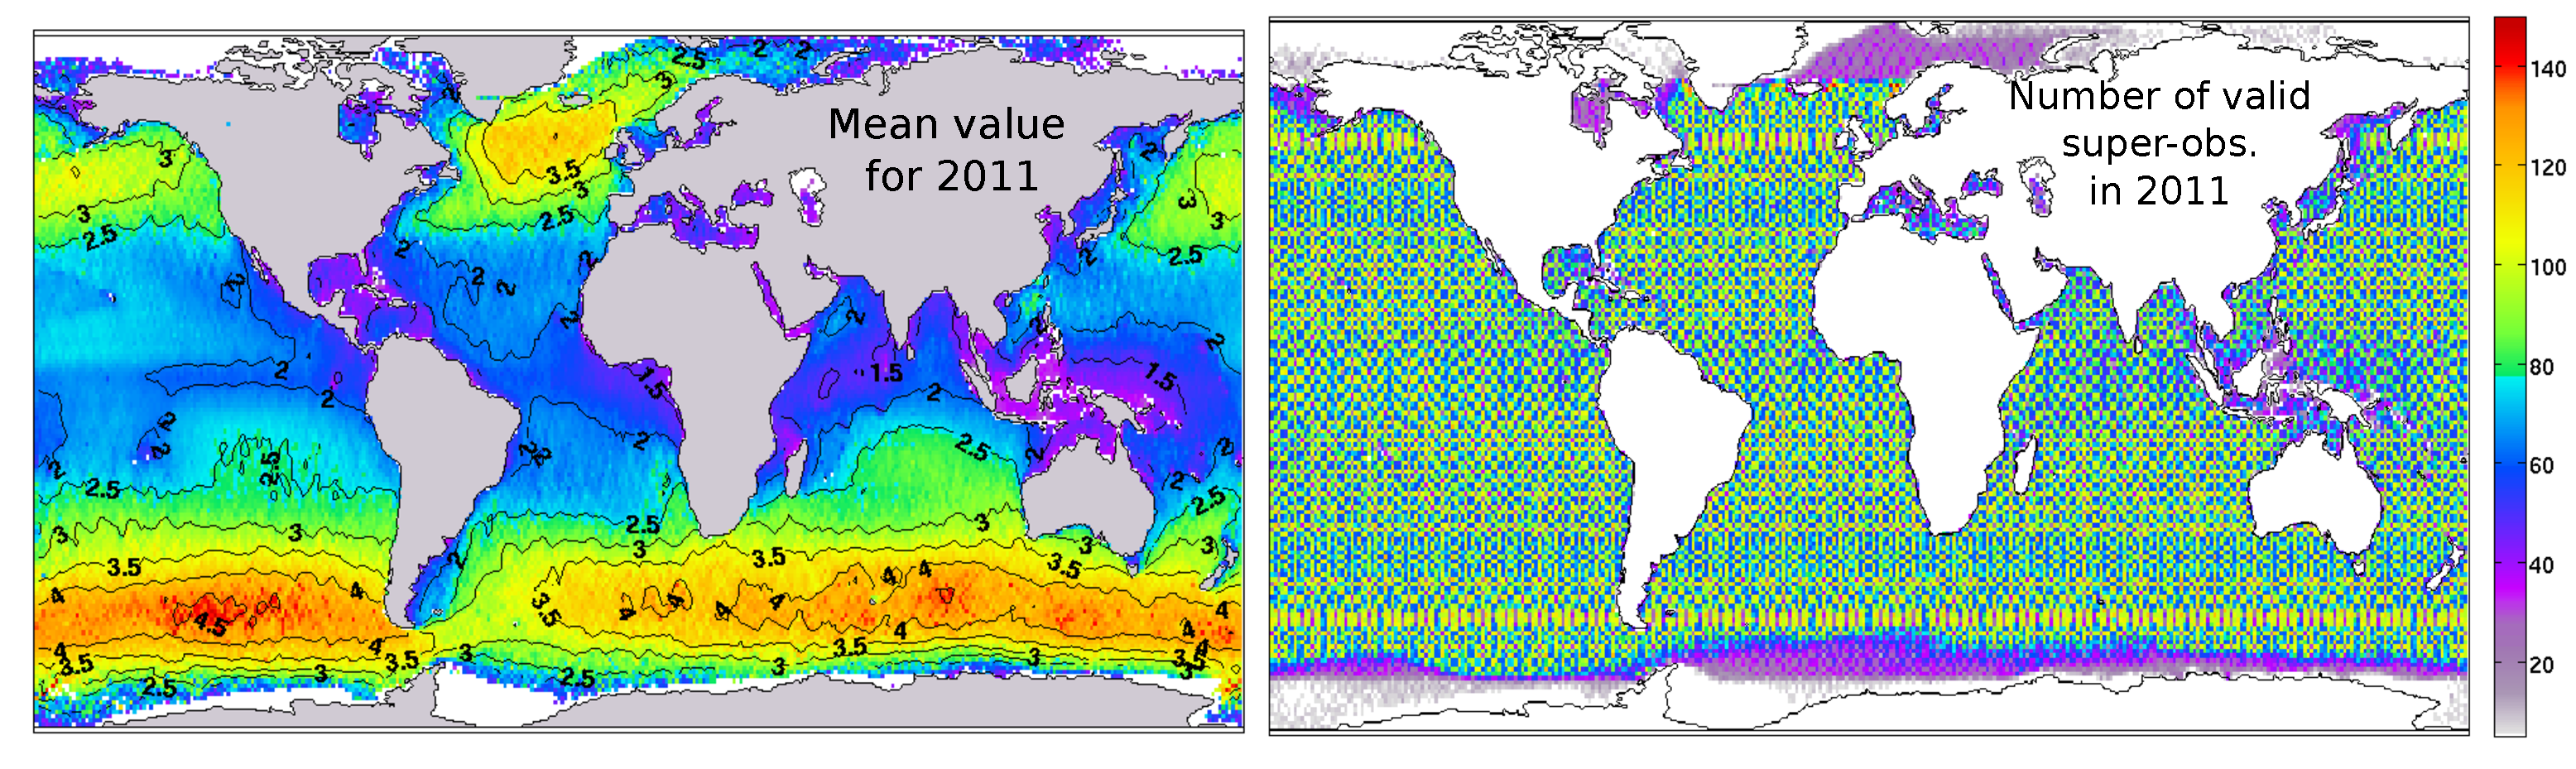
\includegraphics[width=\textwidth]{FIGS_CH_SAT/altimetre_cartes2011.pdf}}
%\vspace{3.64in}
  \caption{Global coverage of satellite altimeters}
    {Over one day, the 3 satellites Jason 2, Cryosat 2 and SARAL/AltiKa covered all the oceans and seas with a density high enough to capture all the 
important storms. In a year, the full ocean is covered at a resolution of 1 degree in latitude and longitude.  
 Data provided by ESA and CNES and processed by Ifremer. The spatial 
cover depends on the orbits shape. The number of tracks per 1 degree x 1 degree box (bottom panel) varies
from 20 to 160 over a year: the coverage is less frequent close to the pole because Jason 2 has a more oblique orbit that does not cover the 
latitudes beyond 66 degrees. Also, sea ice  produces echoes that differ from those of water and prevent the estimation of the wave height.} 
\label{fig:altimeter_coverage}
\end{figure}
%%%%%%%%%%%%% end of figure

Details will vary with different instruments, and here we will use the most simple case of radar altimeters. It was shown by \cite{Chelton&al.1989} that the sea echoes that contribute to the rising part of the waveforms, as shown on Fig. \ref{waveform}, are within a radius $r_C$ of the nadir, the point on the sea surface that is vertically below the satellite, with 
\begin{equation}
    r_C =\sqrt{\frac{ 2 h_o H_s+ 2 \delta_R}{1+h_o/R_E}} \label{eq:rC}
\end{equation}
where $h_o$ is the satellite orbit height above the ground, $R_E$ is the Earth radius and $\delta_R$ is the range resolution of the altimeter.  

\subsection{delay-Doppler altimetry}\label{section:delay-Doppler}
Another principle that can be used to refine the position and/or to measure the velocity of targets along the satellite flight path is the Doppler effect: fixed targets ahead of the radar are moving towards it, and hence have a higher frequency, while fixed targets that are behind along the satellite path 
are moving away, giving a lower radar frequency. Typical low Earth orbits give a satellite velocity around $V=7$~km/s. Hence, a Ka-band system at 36~GHz frequency will see a Doppler shift
of the order of $V f_r/c = 840$~kHz, which is further reduced by the incidence angle $\theta_r$. For a 0.5$^\circ$  antenna aperture, $\theta_r$ will 
normally vary between 0 and 0.5$^\circ$,  and the Doppler will be limited to 7.3~kHz.  

The main benefit of Delay-Doppler altimetry is the increase of the number of "independent looks" of the sea surface, which helps reduce Speckle noise, but cannot do anything about the true geophysical variability induced by wave groups. Delay-Doppler altimetry has also been developed to separate echoes along the track, which is particularly useful for measuring sea ice freeboard at the edges of sea ice leads, hence its first implementation on Cryosat-2. 


A slicing of the radar echoes according to their Doppler shift allows a high-resolution mapping of the surface along the satellite track. 
This principle is used on  Cryosat-2, Sentinel-3, and Sentinel-6 (Mike Freilich) with a standard processing giving 300~m resolution along the track, as shown on figure \ref{waveform}.d. In that case the basic 
data has now one extra dimension, making a `stack' of waveforms. For practical purposes, this stack is converted to a single `SAR mode' waveform, such as the solid lines 
shown in figure \ref{waveform}.b. 
At such a  resolution, the surface elevation due to  very long swells propagating along the track can be resolved. 
A natural limit to this along-track resolving power is the fact that the sea surface is moving up and down with the waves. Indeed, an orbital velocity 
of $w=2$~m/s gives a $u f_r / c=$ Doppler shift that can be mis-interpreted as a difference in incidence angle $\theta_r$ such that  
$(u f_r / c)=(V \sin\theta_r  f_r/c)$, this corresponds to a horizontal displacement $u H_r/V \simeq 200$~m for a radar altitude 
$H_r = 800$~km. 


%\subsubsection{Interferometric systems}



 \subsection{Synthetic Aperture Radars (SARs)}
As  explained, in section \ref{delay}, the separation of echoes in the range direction is easily achieved by combining the delay and frequency modulation of 
the chirped radar signal, with a resolution in distance that is thus controled by the frequency bandwidth. 
In the other direction (azimuth), the simultaneous echoes can be separated by their Doppler shift. 
This is perfect if targets are fixed relative to the ground, and a 
very good resolution can be obtained, both in the range and azimuth directions (about 10~m for Envisat, 5~m for Sentinel 1 in wave mode and 1~m in spotlight mode for TerraSAR-X). This processing 
produces a  map of the surface 
backscatter in delay-Doppler coordinates. Unfortunately these positions are distorted from  true geographic positions when the surface is moving toward the 
radar. With a vertical velocity $w$, targets are displaced by $\delta=w \cos \theta_i  R/V$ along the azimuth direction. With a Sentinel-1 altitude $H_r = 693$~km  and a typical speed over ground $V=7.5$~km/s, when looking at an incidence angle of 23$^\circ$ the distance $R$ is close to\footnote{That approximation assumes a locally flat Earth. The exact value is obtained from the law of cosines in the triangle made of the satellite position, the target position and the center of the Earth, i.e. $R^2 + 2 R R_e \cos \theta_i +R_e^2 - (H_r +R_e)^2=0$, where $R_e$ is the radius of the Earth.} $H_r/\cos \theta_i$ and the 
factor $H_r/V$ is about 92~s$^{-1}$, i.e. a very small velocity  $w= 10$~cm/s gives a displacement in azimuth of $\delta=9.2$~m. 
A high speed train traveling at 100 m/s along tracks at $45^\circ$ with the range direction at an azimuth angle of 23$^\circ$ has a radial velocity of 28~m/s, would be displaced 2.7~km in the azimuth direction, at a location that is 2~km \textit{away} from the tracks!
%Figure \ref{fig:SAR_cars} shows an example of targets displaced from their true locations according to their azimutal speed. 
%
%
%%%%%%%%%%%%% figure
%\begin{figure}[htb]
%\centerline{\includegraphics[width=0.7\textwidth]{FIGURES/SAR_cars.pdf}}
%  \caption{Where is the fast car? it is in the optical picture, but out of the SAR `image'!}
%    {Images of cars with different velocities along an airport runway in a nominally processed radar image (left) and 
%a reference optical image (right), adapted from \cite{Palubinskas&al.2005}. The SAR acquisition was made from a Do-228 aircraft 
%flying at only 88 m/s and altitude 3.94~km, giving a ratio $H_r/V=44$~s$^{-1}$.} 
%\label{fig:SAR_cars}
%\end{figure}
%%%%%%%%%%%%%% end of figure


%%%%%%%%%%%%% figure
\begin{figure}[htb]
\centerline{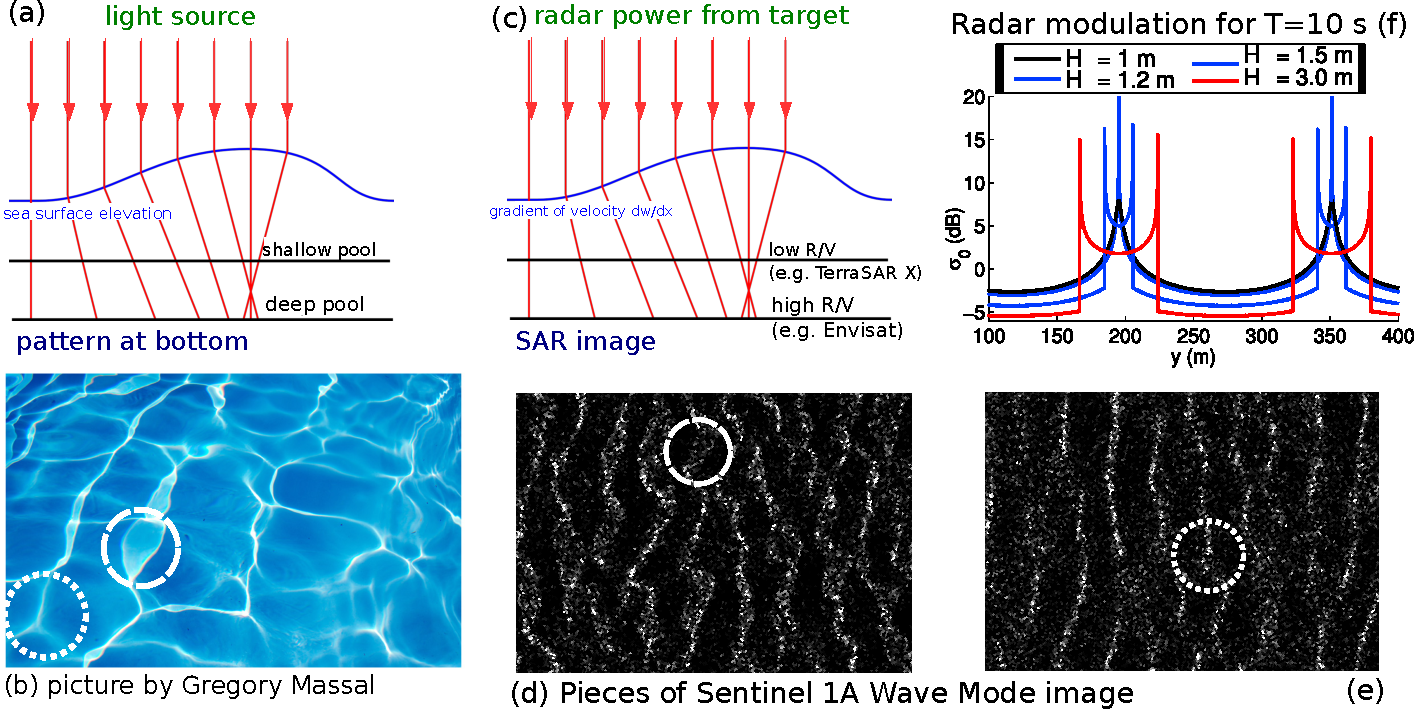
\includegraphics[width=0.8\textwidth]{FIGS_CH_SAT/dessin_fig1_landscape.pdf}}
%\vspace{3.64in}
  \caption{Patterns in SAR images}
    {Analogy between (a,b) light patterns at the bottom of a shallow pool, and (c,d,e) velocity bunching effects
in SAR images of ocean waves. (d) and (e) are taken from a wave mode Sentinel 1A image, acquired on 9 September 2014 at 04:48:16 UTC, 
at 10 and 35~km inside of the sea ice. In (d), almost all crests are doubled, for example in the region within the dashed circle. 
In (e) the lines are less bright and not doubled (for example within the dotted circle). This is easily simulated, as shown in (f), with the variations of image intensity
expected from a sinusoidal monochromatic wave of wavelength 156~m \citep[Adapted from ][]{Ardhuin&al.2017}.} 
\label{fig:SAR_pool}
\end{figure}
%%%%%%%%%%%%% end of figure
In the case of  waves motion a velocity bunching effect appears, the echoes on the image are shifted from their actual
position depending on the surface velocity towards the satellite creating a pattern of brighter areas, where the displaced targets are `bunched 
together', and darker regions. This mechanism is often the main cause of the wave-induced $\sigma_0$ modulation in the open ocean. 
In ice-covered water, this is probably the only mechanism present that creates wave patterns in SAR images. This bunching in the azimuth direction is very 
similar to the light patterns at the bottom of a shallow pool that are caused by light refraction, as illustrated in figure \ref{fig:SAR_pool}. 

%%%%%%%%%%%%%%%%%%%%%%%%%%%%%%%%%%%%%%%%%%%%%%%
%\begin{figure}[htb]
%\centering
%\includegraphics[width=\linewidth]{FIGURES/Nov1_for_book.pdf}
%\caption{Context of the  Sentinel-1A image acquired on November 1st, 2015, at 17:23 UTC, and available in situ data. The full image at 
%full resolution can be viewed at \href{http://bit.ly/22JFruo}{http://bit.ly/22JFruo}. (a) SAR-derived
%roughness (gray scale) showing open water between the Alaska shoreline, to the West of Barrow, and the measurement locations in the red box. 
%(b) Location of the R/V Sikuliaq and some of the measurement buoys. Note that buoy S15 is in open water. 
%(c) piece of the SAR image around the buoys S13 to W3. (d)  Directional spectrum estimated from S15 data using the Maximum Entropy Method.
%(e) Comparison of spectra derived from in situ data and the SAR image around buoy S13 and buoy W3. In each panel the spectrum at the offshore buoy S15 is 
%indicated for reference. The 'cut-off' effect is the reduction of wave spectrum according to eq. (\ref{eq:cutoff}). Adapted from \cite{Ardhuin&al.2017}.}
%\label{fig:nov1}
%\end{figure}
%%%%%%%%%%%%%%%%%%%%%%%%%%%%%%%%%%%%%%%%%%%%%%%
In the case of a monochromatic wave train propagating in the azimuth ($y$) direction, with wavenumber $k_y$, and not located right under the satellite but at an icidence angle $\theta_i$, 
the target displacement in the SAR image due to the velocity towards the satellite is 
\begin{equation}
 \delta = \left ( W \cos (k_y  y - \sigma t) \cos \theta_i  + U \sin (k_y  y - \sigma t) \sin  \theta_i  \right) H_r/(V \cos \theta). \label{eq:delA}
\end{equation}
where $U$ and $W$ are the amplitudes of the horizontal and vertical velocities given by eqs. (\ref{vitesse})-(\ref{eq:w}). 

Assuming a uniform radar power scattered from the sea surface $\sigma_0$, and taking the $y$ dimension  along the azimuth, 
the SAR image intensity is the incoherent sum at the displaced positions $y'$ of the power coming from the true pixel positions $y$, it is thus given by the inverse of Jacobian of the SAR displacements 
$y \rightarrow y'=y+\delta$, \citep[see eq. 21  in][]{Hasselmann&Hasselmann1991}, 
\begin{equation}
 J = \left|dy'/dy\right|,
\end{equation}
for a monochromatic wave of amplitude $a$ it is, 
\begin{equation}
I'_{SAR}(y) = \sigma_0/J = \sigma_0 / \left|1 -  C_{AR}  \sin( k_y y- \sigma t) \right|\label{ISAR}.
\end{equation}
The important parameter for image patterns is the coefficient $c$ in \cite{Alpers&Rufenach1979}, 
\begin{equation}
  C_{AR}=k_y (W + U \tan \theta_i) H_r/V.\label{eq:CAR_def}
\end{equation}


 For $C_{AR} << 1$, eq. (\ref{ISAR}) can be linearized, but as $C_{AR}$ increases, the SAR displacements become strongly nonlinear and for $C_{AR}= 1$, 
 the Jacobian is zero and $I'_{SAR}$ becomes infinite just like the light intensity at the focal point of a lens. 
In our figure 1.f, with a wave period of 10~s traveling in the azimuth direction, $C_{AR}= 1$  corresponds to an amplitude of the elevation $a=0.42$~m, 
which, for random waves of the same energy would be a significant wave height $H_s=4\sqrt(a^2/2)=1.2$~m. 
For $C_{AR} > 1$, each bright line becomes a doublet. The two lines of the doublet progressively drift apart as the amplitude increases, pulling 
the minimum intensity to lower and lower values, up to the point where lines 
from different doublets meet, at $ C_{AR} \simeq 4.6$. Beyond this value there is no region of very low intensity anymore. 
%For waves  in  sea ice, this can be inverted for  $C_{AR}$ less than about 2 to give a map of orbital velocities and from that the wave spectra \citep{Ardhuin&al.2016b}.

In practice, except far inside the  sea ice cover, there are also short wave components in the wave spectrum $E(\kb)$. From a SAR processing point of view, 
these short waves are equivalent to Gaussian random vertical oscillations 
of $<v^2>$ leading to random displacements in the SAR image that are larger than their wavelengths and that do not produce any pattern. These short 
waves also reduce the contrast of longer components. \cite{Hasselmann&Hasselmann1991} gave a theoretical derivation of the impact of random waves on a SAR image spectrum $E_S(\kb)$,
their eq. (55), with a simplified derivation by \cite{Krogstad1992}. In practice the short wave effect is a reduction in the image spectrum by an exponential factor,  
\begin{eqnarray}
 E_S(\kb)&\simeq& \exp(-k_y^2 <v^2> H_r^2/V^2) E_l (\kb) = \exp(-k_y^2 \lambda_c^2/(2 \pi)^2 ) |M_S|^2 \left(E(\kb)+E(-\kb)\right)/2 , \label{eq:cutoff}
\end{eqnarray}
in which $E_l(\kb)$ is a linearized spectrum, based on a modulation transfer function $M_S$ that includes a linearized velocity bunching term, a hydrodynamic term due to the short scattering waves modified by 
longer waves, and a tilt term due to the change in local slope along long waves \citep{Hasselmann&al.1985,Hasselmann&Hasselmann1991}. All terms depend on the incidence angle, 
and these last two terms depend on the polarization of radar waves, horizontal or vertical, and on wind speed and wave age. 
The image is 
completely blurred at the scale of the random displacements and the resolution of 1 or 5~m is useless.


The azimuthal cut-off wavelength is $\lambda_c =  2 \pi \sqrt{<v^2>} H_r/V$, in which $<v^2>$ is the orbital velocity variance.  This cut-off effect is so dominant that it can 
actually be used to measure the surface orbital velocity variance from SAR images \citep{Stopa&al.2016}. A minor difficulty is the separation of the part of the wave spectrum that 
produces patterns in the SAR image and the shorter part that only introduces blurring. Looking at many ERS SAR data, \cite{Kerbaol1997} concluded that, in the case 
of a wind sea, the velocity variance $<v^2>$  should be restricted to waves shorter than a factor $f_L$ times the peak wavelength, with $f_L \simeq 0.33$ for a mean short wave direction 
in the range direction and  $f_L \simeq 0.15$ in the azimuth direction.  

Combining all these effects with some empirically derived MTFs, it was possible to estimate the heights of swells within 25\% of buoy measurements using 
wave mode data from Envisat \citep{Collard&al.2009}. The full significant wave height, including the waves shorter than $\lambda_c$ that are not resolved in the 
SAR image, can also be estimated by combining all image parameters \citep{Li&al.2011}. 






Several aspects of SAR processing are the subject of active research, including the measurement of high winds or currents, and improvements in the estimates of wave 
parameters in particular in ice-covered regions. 

%Figure \ref{fig:nov1} shows an example of waves around the ice edge: in the water (buoy S15), the waves cannot be seen by the SAR 
%because, with a peak wavelength of 100~m, they are much shorter than the 290~m cut-off wavelength. Waves only appear in the ice with an %increasing SAR spectral 
%density which is not due to an increase in wave height, but a reduction in the cutoff wavelength from $\lambda_c = 114$~m at S13 to  $\lambda_c = 87$~m at W3. Hence a correct estimation 
%of $\lambda_c$ is critical for a proper estimation of wave heights either in the open ocean or in ice-covered water. Another important practical problem, especially in ice-covered 
%region, is the presence of non-wave features in the image: boats, slicks, variations in wind speed, leads in ice... these usually show up in the low frequency part of the spectrum, 
%and, in figure \ref{fig:nov1} they probably are the reason for the spurious bump at $f=0.1$~Hz. 
 
Since SAR images are characterized by high resolution (5~m in the Sentinel-1 wave mode, 10~m in Interferometric Wide swath mode), and large coverage, they provide a unique opportunity 
to measure the spatial patterns in the wave field, as shown on figure \ref{SAR_exemple}.

%%%%%%%%%%%%% figure
\begin{figure}[!h]
\centerline{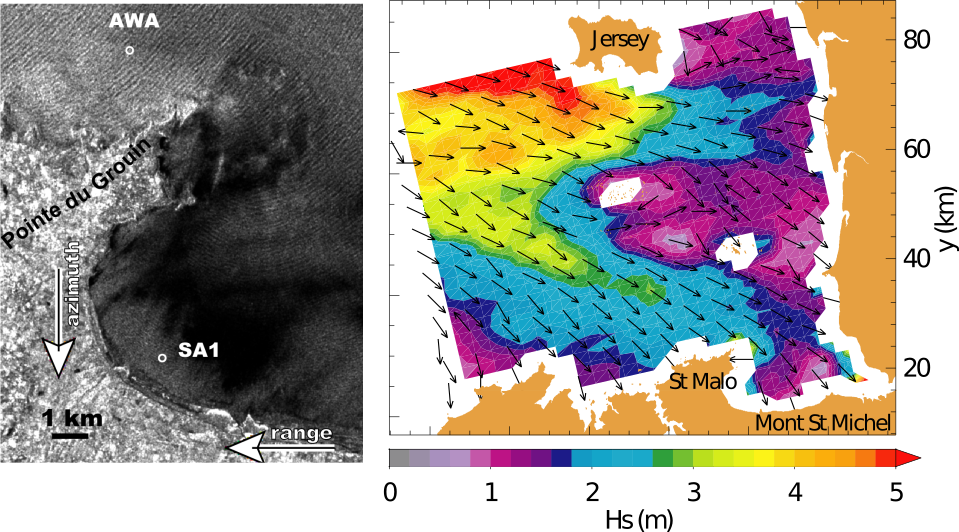
\includegraphics[width=0.8\textwidth]{FIGS_CH_SAT/Image_SAR_Cancale2.png}}
\caption{Left: Sample of a SAR image, recorded by Envisat  on March 9 2003, over French coast. The grey level is a function of the radar cross section that is modulated by waves. 
Right: Full image processed into wave spectra, with significant wave height and peak direction. AWA et SA1 are positions of in-situ instruments, 
used for validation \citep{Collard&al.2005}.}
\label{SAR_exemple}
\end{figure}
%%%%%%%%%%%%% end of figure



\subsection{SAR Across-track Interferometry: SWOT and near-nadir range bunching effects}
Compared to the SAR systems on Envisat and Sentinel-1 described above, the KaRIN instrument on SWOT has two very different features: first it measures at incidences very close to the vertical (nadir), and second it actually has 2 SAR systems forming a cross-track interferometric baseline. This means that in addition to the usual SAR imagery (a little unusual with KaRIN due to their incidence angles) we also get interferograms from the two SAR receivers on KaRIN, which provide a wealth of information: 
\begin{itemize}
\item the mean phase of the interferogram is related to the distance between the radar and the reflecting target, hence the sea surface elevation, which contains the geoid, the dynamic height, tides, internal waves... but also those wind-generated waves that are longer than the SAR pixel, as shown on Fig. \ref{fig:SWOTswell}. 
\item the noise of the interferometric phase is related to the distribution of these distances within a resolution pixel, hence the significant wave height of the waves that are not resolved by the image. 
\end{itemize}

When trying to analyse SWOT data at small scales, it is thus really important to understand what is resolved, what is not, and how the unresolved surface elevations give spurious signals in the resolved part: indeed the imaging of the surface at near-nadir angles meas that all targets that have the same range will fall in the same pixel, even though they are not at the same $(x,y)$ position. This leads to a fairly nonlinear image-blurring or image-enhancing effect called "range-bunching": just like velocity bunching, which distorts or enhances the image in the azimuth direction, range bunching leads to distortions and blurring in range. Figure \ref{fig:SWOTswell} shows some example of wave signatures in SWOT surface elevation maps, that still have to be analyzed quantitatively.
%%%%%%%%%%%%% figure
\begin{figure}[htb]
\centerline{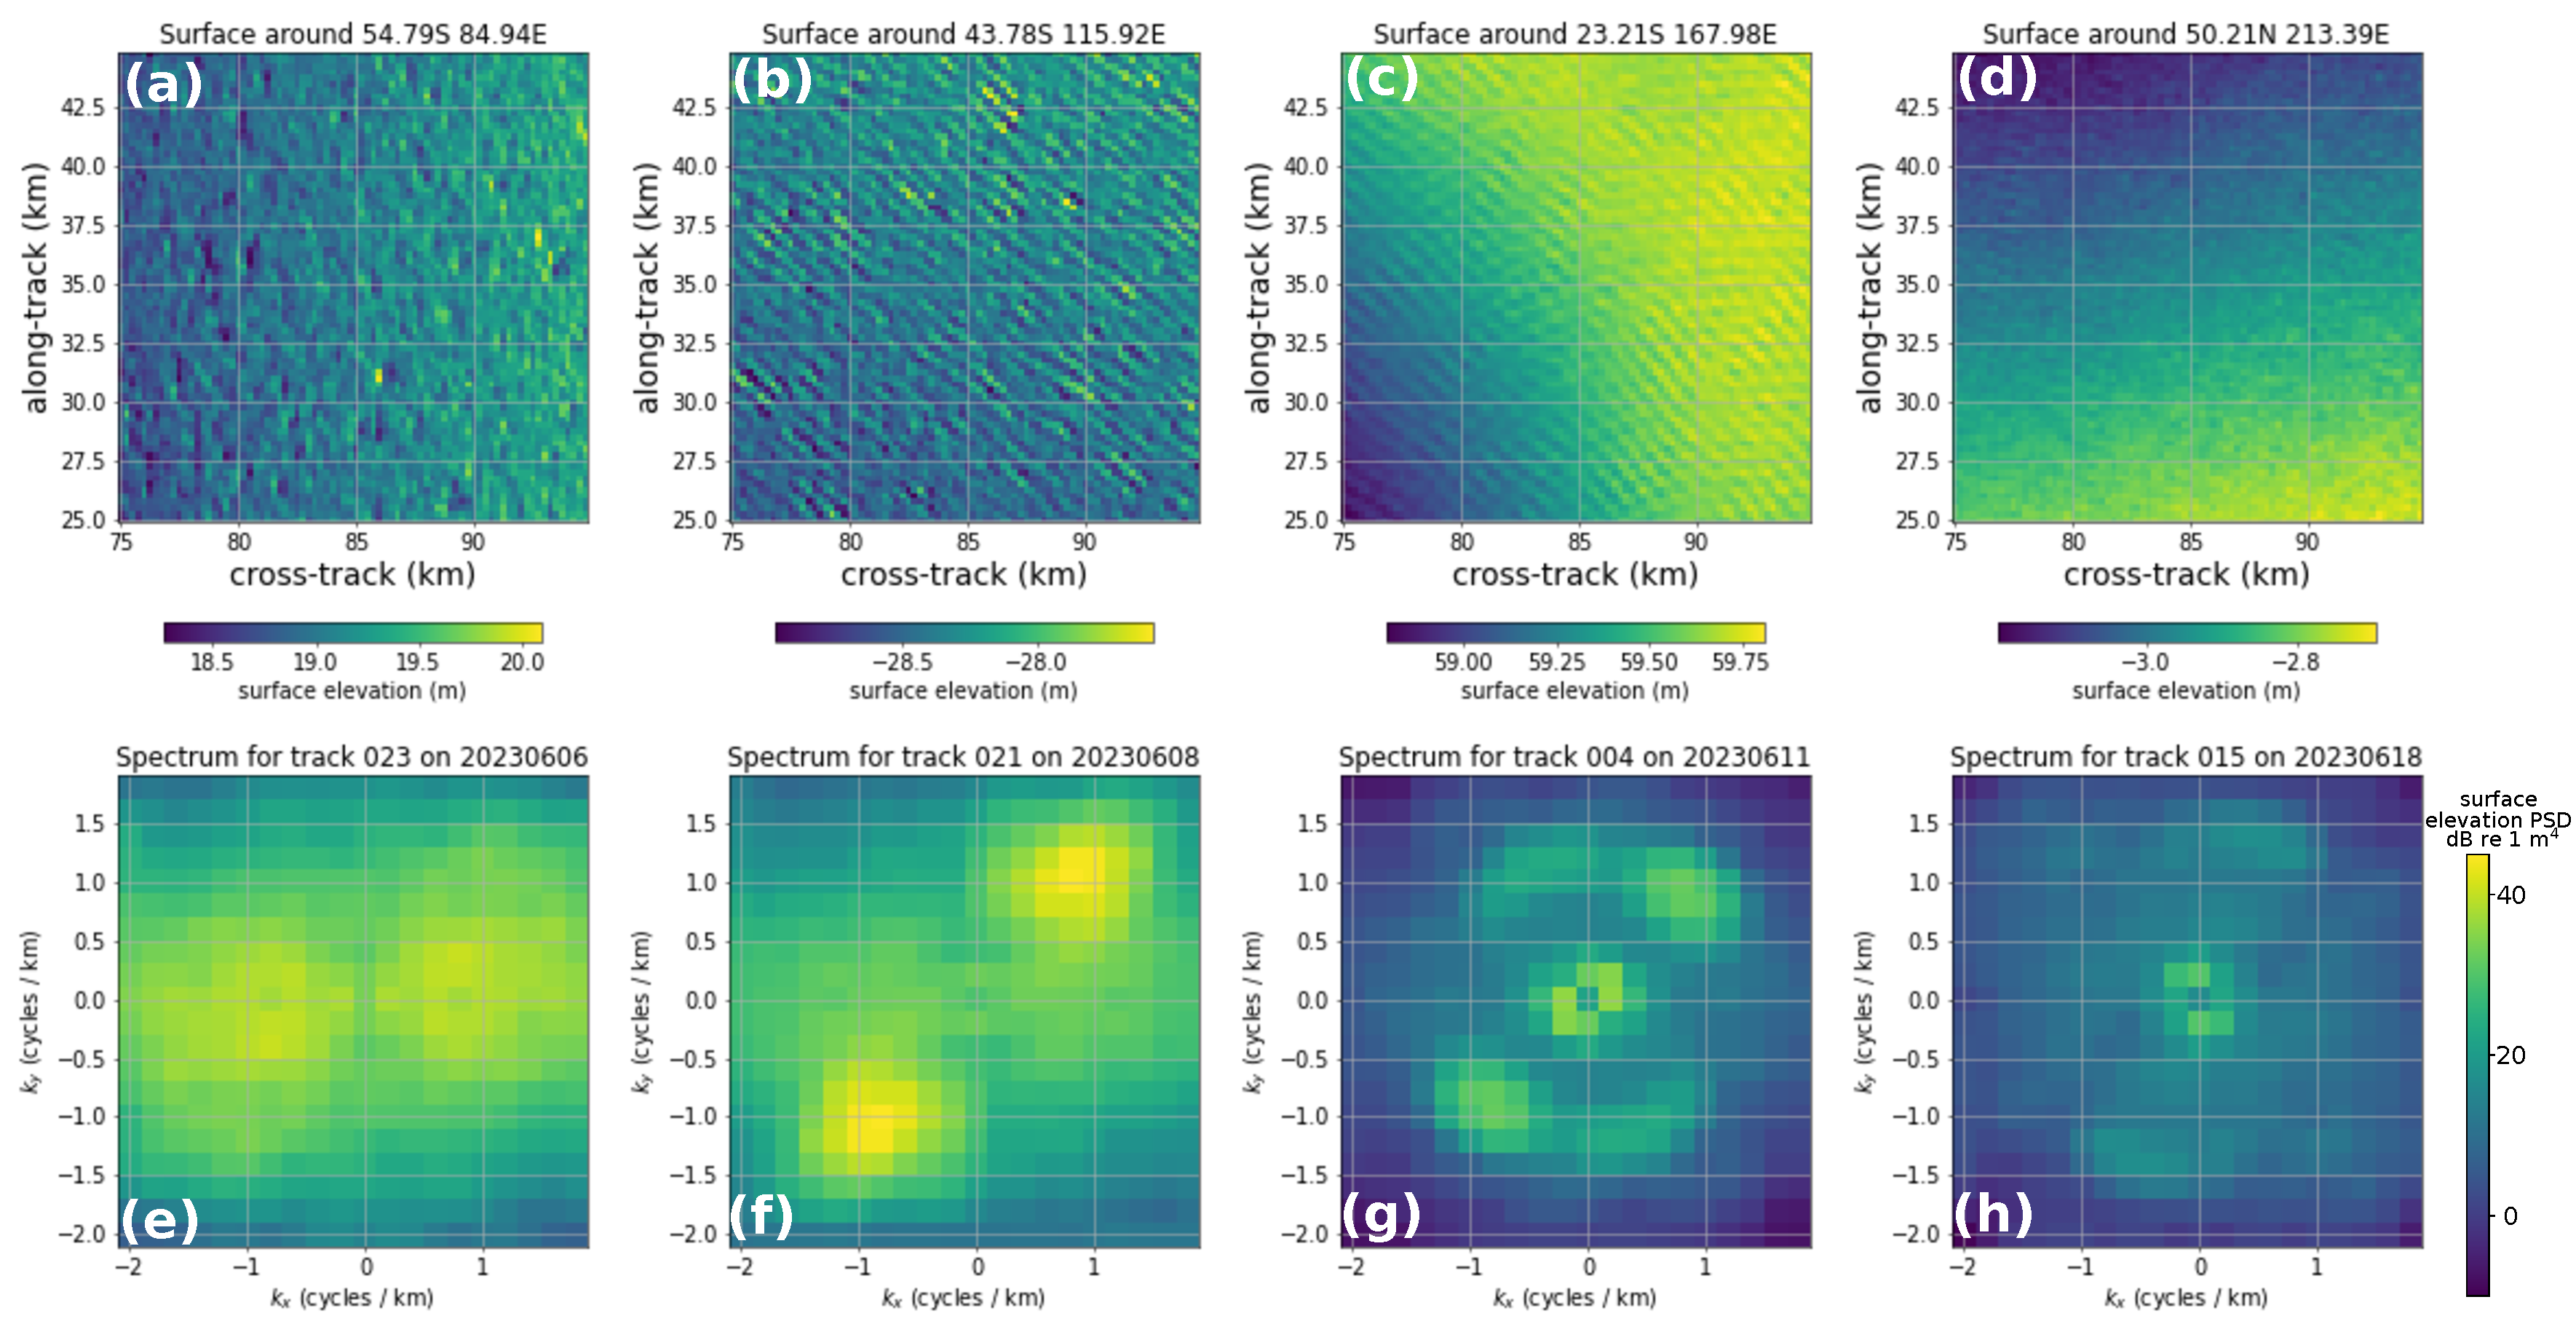
\includegraphics[width=\textwidth]{FIGS_CH_SAT/SWOTSWELL.pdf}}
\caption{Following swells with SWOT, from storm to the antipodes}{Top: small pieces (20 by 20 km) of SWOT data, bottom: corresponding surface elevation spectra $E(k_x,k_y)$, these are double-sided spectra. Left: in the storm on June 6 2023, south of Kergulen islands with strong range bunching effect. Next: large swells South of Australia, June 8. Next: refraction and diffraction over Antigonia seamount, south-east of New Caledonia, June 11. Right: small amplitude swells at ocean station Papa, Gulf of Alaska, on June 18, after 17,000~km of propagation.}
\label{fig:SWOTswell}
\end{figure}
%%%%%%%%%%%%% end of figure
You may look at the work by \cite{Peral&al.2015} before a more detailed summary appears in this section or a new chapter. 

\subsection{The wave spectrometer and the matching wavefront technique}
Whereas a SAR resolves the wave patterns in an image to produce a wave spectrum, 
it is possible to measure the 2D wave spectrum from a combination of 1D wave spectra. 
%%%%%%%%%%%%% figure
\begin{figure}[htb]
\centerline{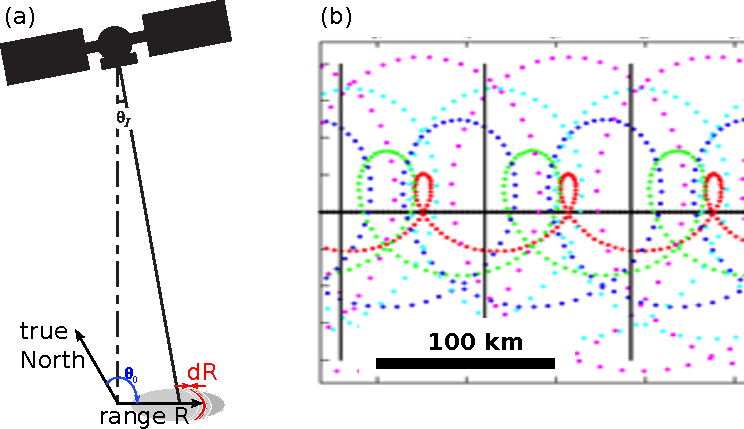
\includegraphics[width=0.4\textwidth]{FIGS_CH_SAT/CFOSAT_v2.pdf}}
\caption{Measurement principle  the SWIM radar that on CFOSAT. (a) geometry of the measurements for one cycle 
in direction $\theta_0$. The resolution in range $dR$ is of the order of 10~m, but the azimuth resolution is 18 km. Using different incidence angles $\theta_I$ (0, 2, 4, 6, 8 and 10 degrees) 
and rotating around the nadir provides estimates $E(k,\theta_0)$ in all direction $\theta_0$. (b) Coverage of the SWIM instrument on CFOSAT: each colored dot is the center 
of a 19~km diameter footprint.}
\label{CFOSAT}
\end{figure}
%%%%%%%%%%%%% end of figure

When echoes are combined from narrow strip in range (red band in figure 
\ref{CFOSAT}.a), the Fourier transform of these echoes in the range direction selects only the modulations by waves that are perfectly aligned with the direction 
$\theta_0$ to which the radar is looking, all other components cancel out.  Hence, the Fourier analysis of radar echoes provides a 1D spectrum  $E(k,\theta_0)$  
in the look direction. 
A successive acquisition in different directions provides the full directional spectrum $E(k,\theta)$.  
This is the principle of the wave spectrometer and it has been demonstrated with the airborne instrument
RAWS, developed by NASA \citep{Jackson&al.1985}, STORM and KuROS developed jointly by CNES and CNRS \citep{Hauser&al.1992,Caudal&al.2014}.
The first satellite wave spectrometer is SWIM, and it flies on the China-France Ocean Satellite (CFOSAT, Figure \ref{CFOSAT}), which was launched on October 29, 2018 \citep{Hauser&al.2021}. SWIM is unique in providing wave spectra co-located with classical altimeter measurements, allowing a a much better understanding of historical altimeter data and their along-track variability \citep{DeCarlo&al.2023}, as detailed in chapter \ref{ch_groups}. 

%For larger incidence angles, the measurements cover a larger area of the ocean, but there is more sensitivity to the wind speed in the radar back-scatter. Hence, the SWIM  design is limited to 10 degrees of incidence. A larger incidence also requires a more powerful radar, because the reflectivity decreases with incidence angle. 

It is also possible to analyze the Doppler of the backscattered signal, as demonstrated with KuROS \citep{Caudal&al.2014}, but this is best done with a narrower antenna pattern as used from space. This additional measurement allows to remove the 180 degree ambiguity on the 
wave propagation direction, but it also provides an indepedant measuremnt of the wave spectrum via the orbital velocities, and finally it contains the signature of 
surface currents.  This Doppler capability to measure currents was included in the SKIM concept \citep{Ardhuin&al.2019e} and demonstrated with airborne measurements \citep{Marie&al.2020}.



\cleardoublepage
\chapter{Measured wave evolution: main parameters and wave spectra}\label{ch3}
\input{ch4_en}
\cleardoublepage
\chapter{Physics of spectral wave evolution: deep water}\label{ch_sourceterms}
\input{ch5_en}
\cleardoublepage
\chapter{Waves and momentum}\label{ch_momentum}
\input{ch_qdm_en}
\cleardoublepage
\chapter{Wave-current interactions}\label{ch_courant}
\input{ch_courant_en}
\cleardoublepage
\chapter{Interactions of waves and sea ice}\label{ch_ice}
\input{ch_ice_en}
\cleardoublepage
\chapter{Numerical modeling in deep water}\label{ch_model}
\input{ch_model_global_en}
\cleardoublepage
\chapter{Extreme waves and historical storms}\label{ch_histo}
\input{ch_histo_en}
\cleardoublepage
\chapter{Air-sea interactions: \\ wind stress and mixing}\label{ch_ioa}
Fluxes of any quantity (momentum, heat, mass, carbon dioxide or other gases ...) between the ocean and the atmosphere is very often parameterized as the difference in the volumic density of this quantity between the air and atmosphere, multiplied by an exchange coefficient. This exchange coefficient itself is generally parameterized as a mean velocity difference across the air-sea interface, for practical reason the norm of the vector difference of the wind at 10~m height $\Ub_{10}$  minus the quasi-Eulerian current at some depth $\widehat{\ub}$ multiplied by a non-dimensional exchange coefficient $C_e$. That coefficient generally represents the full complexity of the ocean surface, the presence of bubble in the water, spray in the air, and the geometry of the interface. Because turbulent transport can be much more efficient, the proper scale for trhe velocity is rather the friction velocity $u_\star$, which means that generally $C_e \ll 1$. The magnitude of this exchange has profound impact on both the ocean and atmosphere, and natural phenomena such as hurricanes are very sensitive to exchanges of heat and momentum.  Here we will particularly focus on the fluxes of momentum and energy, looking only at their impact ont the ocean. In general the feedback on the atmosphere cannot be neglected. 

A self-similarity theory of turbulence in which big eddies feed smaller eddies following Kolmogorov, gives the Monin-Obukhov  theory for the turbulence and associated fluxes in the atmospheric and marine boundary layers \citep{Monin1962,Zilitinkevitch&Chalikov1968}. This was well verified over land \citep{Businger&al.1971}, and in particular it is usual to correct the wind speed  $\Ub_{10}$ to a neutral wind speed 
$\Ub_{10N}$ to take into account the source of turbulence coming from buoyancy, in the unstable case of warm water under cold air. A detailed account can be found in \cite{Schlichting1979}. 

The ocean mixed layer in its top few meters is strikingly different from the atmospheric side, due to the extra source of turbulence coming from ocean waves, mostly due to wave breaking but also associated to the strectching of turbulence by the Stokes drift. This was only revealed in the 1990s and the full details are still being explored, including the interaction of boundary layer turbulence with ocean fronts, internal waves  and other features \citep[e.g.][]{Suzuki&al.2016}. 

\section{Sea state influence on air-sea fluxes}


\subsection{Wind stress and drag coefficient}
For the horizontal momentum, which is a two-component horizontal vector $(U,V)$, the flux is a also vector $(\tau_x,\tau_y)$ and the exchange coefficient that relates these two quantities $C_e$ should generally be a tensor. However, it is most often replaced by a scalar $C_{DN}$ parameterized as follows, which makes the big assumption that the flux vector, which is usually called "wind stress", is aligned with the wind vector at 10~m,  
\begin{equation}
 {\bm{\tau}}=\rho_a C_{DN} U_{10N} \Ub_{10N},
\end{equation}
where the neutral wind speed is the equivalent wind speeds that gives the same stress in the atmospheric stratification is neutral. It was found in most experiment that $C_{10N}$ tends to be higher for relatively young waves as shown in figure \ref{Drennanetal2003}.
%%%%%%%%%%%%%%%%%%%%%%%%%%%%%%%
\begin{figure}
\centerline{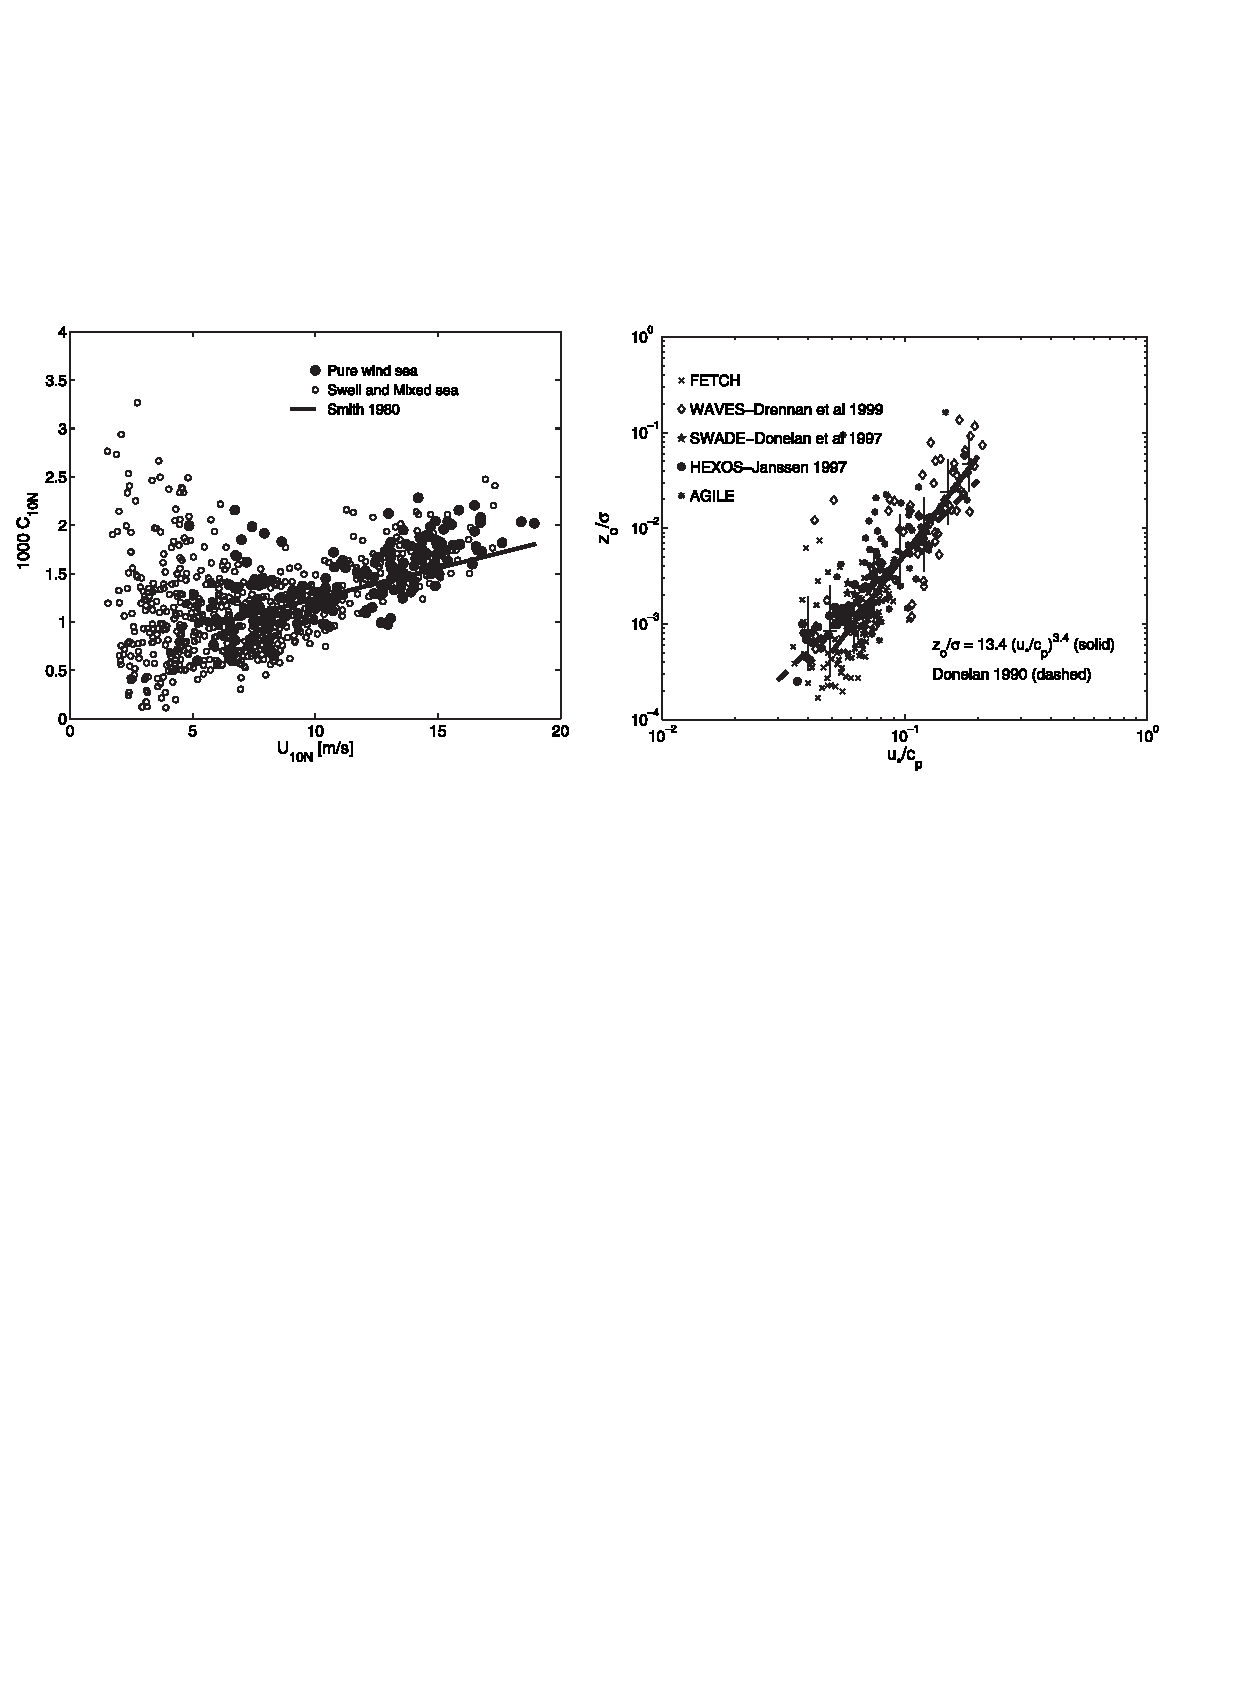
\includegraphics[width=\textwidth]{FIGS_CH_AIRSEA/Drennan_etal_JGR2003.pdf}}
%\vspace{3.64in}
  \caption{Effect of sea state on the wind stress.}{Left: measured neutral drag coefficient  $C_{10N}$, 
  during the  FETCH experiment in the Mediterranean. Right: variation of the roughness length  $z_0$, normalized by a typical wave amplitude $\sigma=H_s/2$ for various experiments. Figure reproduced from \cite{Drennan&al.2003}.}
\label{Drennanetal2003}
\end{figure}
%%%%%%%%%%%%%%%%%%%%%%%%%%%%

However, in general the wave age is correlated to the wind speed, so that it is very difficult to isolate wave age effects. In their recent review of wind stress parameterization for wind speeds 0 to 25 m/s, \cite{Edson&al.2013} concluded that the updated COARE 3.5 parameterization gives a good reproduction of the wind stress as a function of the neutral wind speed alone. 

For higher wind speeds, several estimates of the stress suggest that the value of $C_d$ may decrease, possibly associated to a full separation of the boundary layer. Figure \ref{Lucia2017} shows several drag coefficient from observations and as used in the ECMWF atmospheric model, for which the drag takes into account the waves \citep{Janssen2004}. %Interestingly the ECMWF drag is relatively high and the ECMWF winds are relatively low compared to measurement from platforms. 
%%%%%%%%%%%%%%%%%%%%%%%%%%%%%%%
\begin{figure}[h]
\centerline{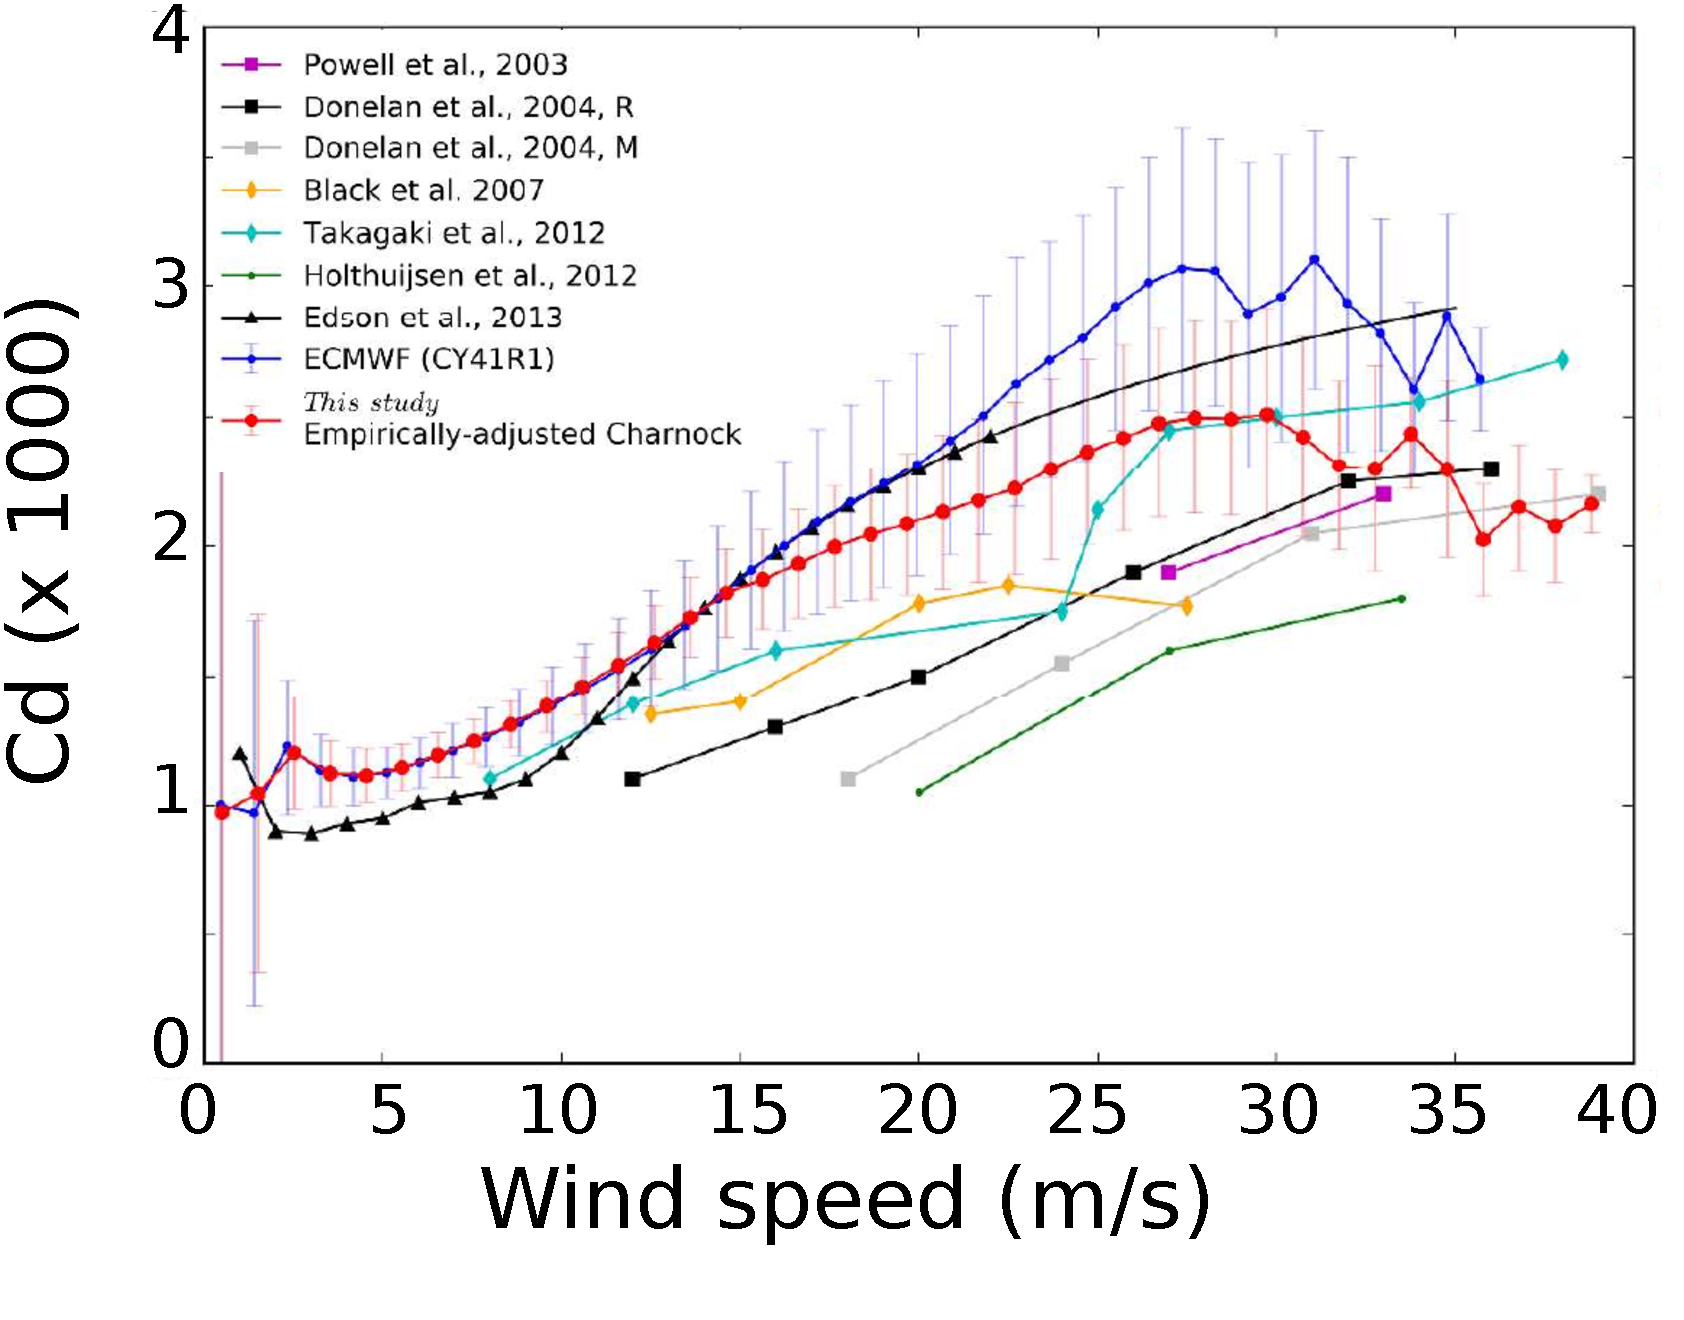
\includegraphics[width=0.6\textwidth]{FIGS_CH_AIRSEA/High_drag_coeff.pdf}}
%\vspace{3.64in}
  \caption{Left: Comparison of drag coefficient for ECMWF (CY41R1) parameterization, empirically-adjusted Charnock parameterization and observations (Donelan et al., 2004, 'R' or 'M' corresponds to different measurements techniques Reynolds or Momentum Budget. %Right: Wind speed biases, on the period 23 to 27 of January 2014 on North East Atlantic, between (a) ASCAT-KNMI, (b) ASCAT-RSS, (c)AMSR2, (d) WindSat, (e) buoys, (f) platforms and model for the default ECMWF CY41R1 (blue) and empirically-adjusted (red) parameterizations.  
%  Beyond 30~m/s, values are plotted as points, representing the large uncertainties on observations.  
  Adapted from \cite{Pineau-Guillou&al.2018}.}
\label{Lucia2017}
\end{figure}
%%%%%%%%%%%%%%%%%%%%%%%%%%%%
%We also note that wind speeds derived from satellite radiometers and scatterometers are not direct measurements and thus depend on the choice and tuning of a Geophysical Model Function that translates the measured quantity (brightness temperature or backscatter) into wind speed. For example the winds from the ASCAT scatterometer processed by KNMI and RSS differ by 7 m/s on average for 30 m/s winds. 

\subsection{Swell and stress direction}
Besides the magnitude of the wind stress, waves also modify the stress direction. This is particularly noticeable at low wind speeds in the presence of swell. Indeed, the wind stress may be opposite to the wind direction for wind speeds below 3 m/s, as the wave are loosing momentum to the atmosphere and generating a low-level jet of wave-driven wind \citep{Semedo&al.2009,Hogstrom&al.2009}. It is more frequent to observe systematic deviations of the wind stress and wind speed directions when waves and wind are not aligned \citep{Potter&al.2015}. 

\subsection{Other effects}
Waves generally have an impact on all air-sea exchanges, not just momentum. This includes mass fluxe \citep[see][ for a recent review of spray generation]{Veron2015} and gas transfer \citep[e.g.][]{Brumer&al.2017b}. Also in the presence of an ice layer, wave-ice interactions should be taken into account. These are discussed in chapter \ref{ch_ice}. 

\section{Drift and mixing}
\subsection{Momentum flux for the Eulerian mean current}
Knowing the wind stress is a first step in determining how the ocean is forced, but this is not enough to tell how much of that momentum goes into currents as most of it generally goes through the wave field. It is only when the wave momentum is constant that the momentum flux from the wind goes entirely to the ocean circulation. In general, we can use the wave energy balance with source terms $S_{\rm in}$ and $S_{\rm dis}$ presented in Chapter \ref{ch_sourceterms}, to compute the wave momentum balance. This was done at the end of Chapter \ref{ch_current}, when we introduced the momentum flux from wind to waves $\tau^{\mathrm{aw}}$ and the flux from waves to ocean $\tau^{\mathrm{wo}}$ .

\subsection{Quasi-Eulerian currents}
The interaction of waves and currents is the topic of onging research, in particular the effects of vertically sheared currents on the waves. 
A general description of these interaction in three dimensions is given in Part 3. Here 
we will consider the much more simple case of a horizontally homogeneous ocean. The wave-averaged momentum equation for the mean current $ \widehat{\mathbf u}$
then takes the following form \citep{Hasselmann1970,Xu&Bowen1994}, 
\begin{equation}
 \frac{\partial \widehat{\mathbf u}}{\partial t}
  = 
 - f {\mathbf e}_z \times \left(\widehat{\mathbf u}+{\mathbf U}_{s}\right) + \frac{\partial}{\partial z} \left[{K_z} \frac{\partial
\widehat{\mathbf u} }{\partial z}\right] - {\mathbf T}^{\mathrm{wo}} 
 \label{avgmomz2}
\end{equation}

The solution is determined by the surface boundary conditions, and the profiles of the mixing coefficient $K_z$,  
and the total momentum injected by the waves ${\mathbf T}^{\mathrm{wo}}$ which is a depth-distributed force such that the momentum flux is 
\begin{equation}
\tau^{\mathrm{wo}}_{\alpha} = \int_{-h}^{\overline{\zeta}} T^{\mathrm{wo}}_{\alpha} {\mathrm d}z = \int \frac{\rho_w g}{C}\left[ S_{\mathrm{tot}}(f,\theta) -S_{\mathrm{atm}}(f,\theta)  \right] {\mathrm d}f {\mathrm d} \theta 
 \end{equation}
 with the source terms $S$ defined in Chapter \ref{ch_sourceterms}. 
 
The current can be obtained by solving  (\ref{avgmomz2}) with a turbulent closure that gives an estimate of  $K_z$. 
Following Prandtl (1904), the usual turbulence closure has an addy viscosity that increases with the distance from the boundary 
\citep{Schlichting1979} and involves a velocity scale $q$ associated to the turbulent motion, 
\begin{equation}
K_z = q S_M l,
\end{equation}
where the turbulent kinetic energy per unit mass is  $q^2 = \overline{u^\prime_i u^\prime_i}$, $S_M \simeq 0.39$ is a constant. 
With this, the  most simple model uses a prescribed mixing length $l$ that is the maximum distance from the surface or the base of the mixed layer. 
\begin{eqnarray}
l &= &\max\left\{-\kappa D_m \varsigma, \kappa  z_{0-}\right\} \quad
\textrm{for}
\quad (-h+\overline{\zeta})/2 < z < \overline{\zeta} \nonumber\\
l &= &\max\left\{\kappa D_m (1+\varsigma), \kappa z_{0b}\right\} \quad
\textrm{for} \quad   -h < z  <(-h+\overline{\zeta})/2 ,
\end{eqnarray}
where $D_m$ is the thickness of the mixed layer. The roughness length  $z_{0-}$ yields a non-zero value of  $K_z$ at the surface, 
  which is consistent with measurements \citep[e.g.][]{Kitaigorodskii1994}. \cite{Thorpe&al.2003a} 
  and other authors have suggested that $z_0$ is of the order of  $H_s$, the significant wave height, and should be more precisely related to the height of the breaking waves\footnote{Ocean circulation models before the year 2000 
  used to ignore these effects, and could have very small values of $K_z$ at the surface, e.g. \citet{Large&al.1994}, 
which could give highly unrealistic values of the surface drift when using very high vertical resolutions.}. 

More complex models consider also an equation of evolution for $q$,  and one must also define the surface boundary
condition for $q$. For example  \cite{Mellor&Yamada1982} use the following equations
\begin{eqnarray}
l q S_q \frac{\partial q^2}{\partial z}  =  \alpha_{\mathrm{CB}} \frac{\rho_a^0}{\rho_w^0}
u_\star^3  \quad \textrm{at} \quad \varsigma =
0, \label{surfq} \\
l q S_q \frac{\partial q^2}{\partial z}  =0 \quad \textrm{at} \quad \varsigma =
-1,
\end{eqnarray}
where $S_q=0.2$. The mixing coefficient for $q^2$ is  $l q S_q$, and 
$\alpha_{\mathrm{CB}}$ is the ratio of the energy flux coming from ocean waves (presumably due to wave breaking), and the fruction velocity cubed. 
This coefficient was particulary discussed by \cite{Craig&Banner1994} and many following authors 
\citep{Terray&al.2000,Mellor&Blumberg2004,Rascle&Ardhuin2009,Rascle&Ardhuin2013}. 
Typically $\alpha_{\mathrm{CB}}$ is of the order of  $100$.

For a simple estimation we consider a fully developed sea state, and we assume that   ${\mathbf
T}^{\mathrm{wo}}$ is concentrated near the surface so that  
we can replace these terms in 
(\ref{avgmomz2}) by a local source of momentum in the surface boundary condition. Namely the net momentum flux coming from the wind and waves is balanced by vertical mixing, 
\begin{equation}
{\mathbf \tau}_a - \tau_{\alpha}^{\mathrm{aw}} + \tau_{\alpha}^{\mathrm{wo}}=
 \rho_w K_z \frac{\partial
\widehat{u}_\alpha}{\partial \varsigma} \quad \textrm{on} \quad \varsigma =0.  \label{surfstress3}
\end{equation}
In fact, in the presence of a strong surface mixing the numerical solution is not very sensitive to the forcing in the boundary condition 
or as a body force concentrated near the surface \citep{Rascle&al.2013}. 

Assuming a fully delveloped sea state the momentum flux $\tau_{\alpha}^{\mathrm{aw}} $  that goes to the wave growth is canceled 
by the dissipation terms and we have
\begin{equation}
{\mathbf \tau}_a  = \rho_w u_\star {\mathbf u}_\star = \rho_w K_z
\frac{\partial \widehat{u}_\alpha}{\partial \varsigma} \quad \textrm{on} \quad
\varsigma = 0, \label{surfstress4}
\end{equation}
with $u_\star$ is the wind friction velocity.

%%%%%%%%%%%%% figure
\begin{figure}
\centerline{\includegraphics[width=\textwidth]{FIGS_CH_AIRSEA/profil1_en.pdf}}
  \caption{Upper ocean current profiles for a wind speed $U_{10}=10$~m/s}
 {(a) Profiles with a very low value of $z_0$, representing an unrealistic situation without waves 
  (b) profiles with a realistic value of $z_0$. In terms of drift velocity, the much lower value of the surface current is compensated 
  by the Stokes drift.  The velocity scale $q$ is the square root of the turbulent kinetic enenergy (TKE). A realistic surface flux of $q$ is
  needed to get the realistic TKE profile in (b).  (Figure courtesy  of Nicolas Rascle).} \label{fig:2}
\end{figure}
%%%%%%%%%%%%% end of figure

Until the 1990s, all ocean circulation models used very small values of mixing at the surface \citep[e.g.][]{Large&al.1994}, corresponding 
here to low values of $z_{0-}$, such as in Figure \ref{fig:2}.a. This can give very high values of the surface current,s depending on the vertical resolution, 
up to the usally observed 3\% of the wind speed 
\citep{Huang1979} or more. But \cite{Agrawal&al.1992} found that the disspation of TKE was much higher in reality, by at least 
one order of magnitude, so that the mixing must have been strongly underestimated.  Recent models have clearly shown that 
higher surface mixing values are more realistic. For example \cite{Mellor&Blumberg2004} use  $z_0=0.8 H_s$ to get a better fit to measure sea surface temperatures 
in the Gulf of Alaska. This gives a much weaker surface quasi-Eulerian velocity.  This mixing induced by wave breaking is particularly important for 
relatively shallow mixed layers such as found in the Arabian Sea in summer \citep{Janssen2012}, or caused by the diurnal cycle of heating \citep{Noh1996,Noh&Kim1999}.

%%%%%%%%%%%%% figure
\begin{figure}
\centerline{\includegraphics[width=0.4\textwidth]{FIGS_CH_AIRSEA/Terray_etal2000_p5.pdf}}
  \caption{Quasi-Eulerian velocities near the sea surface.}{Two types of current-meters  (SASS and VMCM) provide mean current velocities that have been corrected for wave motion. $u_{\star w}=(\rho_a/\rho_w)^{1/2} u_{\star}$ is the friction velocity in the water (Figure from Terray et al. 2000)\nocite{Terray&al.2000}. The difference in current velocity between the surface and the thermocline is of the order of  0.5\% 
  of the wind speed $U_{10}$.} \label{fig_Santala}
\end{figure}
%%%%%%%%%%%%% end of figure
There are very few measurements of velocity profiles of Eulerian or Lagrangian velocity within the upper 
few meters of the surface. Observations by \cite{Santala&Terray1992} show an Eulerian current that does not exceed  0.5\% of the wind 
speed, see fiugre
\ref{fig_Santala}. 
How general is that? Is it still true if we can measure within a few centimeters of the surface, or right at the surface? 
This is not known yet but several techniques using thermal imagery or polarimetry and wave dispersion should be able to answer these questions. 


\subsection{Stokes drift}
The difference between the Lagragian mean velocity, which is the speed or water particles and the speed that advects tracers (temperature, salinity ...), and the quasi-Eulerian velocity is the Stokes drift. To lowest order, this Stokes drift can be computed from the wave spectrum (Chapter \ref{ch_momentum}). For random wave field in deep water, eq. (\ref{eq:Us_mono_deep}) gives \citep{Kenyon1969},
\begin{eqnarray}
 U_s (z)&=& \int\int 2 \sigma k \cos(\theta) E(f,\theta) \exp(2kz) {\mathrm d}f {\mathrm d} \theta, \\
 V_s (z)&=& \int\int 2 \sigma k \sin(\theta) E(f,\theta) \exp(2kz) {\mathrm d}f {\mathrm d} \theta.
\end{eqnarray}
%%%%%%%%%%%%%%%%%%%%%%%%%%
\begin{figure}[htb]
\includegraphics[width=0.9\linewidth]{FIGS_CH_AIRSEA/Us_PAPA_62069_line.pdf}
\caption{Example of mean value (in red) of the surface Stokes drift vector norm $U_{ss}=|(U_{ss},V_{ss})|$ as a function of wind speed for two locations: station PAPA in the North-East Pacific, and buoy 62069 off the French Atlantic coast. These are obtained by integrating the wave spectrum up to 0.5~Hz. The black symbols show the mean plus or minus one standard deviation for each wind speed. The dashed grey line is $U_S = 0.01 U_{10}$.   \label{fig:USU10}}
\end{figure}
%%%%%%%%%%%%%%%%%%%%%%%%%%


Clearly this expression has a strong contribution from short waves, and thus should be largely influenced by the local wind. 
Still, for any given wind speed, the surface Stokes drift value $U_{Ss}$ has a root mean square variability of the order of 40\%, particularly for relatively low wind speeds, below 7~m/s, as shown in figure \ref{fig:USU10}.

Based on direction spectra measured by surface-following buoys, 
\cite{Ardhuin&al.2009} found that the surface Stokes drift  $U_{\mathrm{Ss}}$ could be estimated fairly accurately, with a root-mean-square error of the order of 20\%, by an expression as a function of the wind speed and wave height, 
\begin{equation}
U_{\mathrm{Ss}}(f_c)\simeq 3.7\times 10^{-4}
\left[1.25-0.25\left(\frac{0.5}{f_c}\right)^{1.3}\right] U_{10}
 \min\left\{U_{10},14.5\right\} + 0.025\left(
H_s-0.4\right),\label{Uss_U10}
\end{equation}
in which  $f_c$ is the frequency up to which the Stokes drift is taken into account. This 
expression was validated for $0.3<f_c<0.6$~Hz. 




When subtracting this Stokes drift from HF radar data they found that the quasi-Eulerian current was of the order of 0.4 to 0.8\% of the wind speed, with important variations due to inertial oscillations, and, in the Northern hemisphere, a mean direction 60 degrees to the right of the wind. The model proposed here adds the Stokes drift to the quasi-Eulerian velocity and matches relatively well observations of surface drift and mixing  \citep{Rascle&al.2006}. The effect of stratification is particularly discussed by \cite{Rascle&Ardhuin2009}. 

The present model gives both a strong vertical shear of the drift velocity (mostly due to the Stokes drift) and a strong mixing (caused by wave breaking). 
Still the modeled drift is low by  0.5 to 1.5\% of $U_{10}$ compared to the typical 3\% surface drift. One possible reason is that surface drift objects are trapped in convergence zones where the mean velocity is faster than that of the surrounding water. These convergence zones are associated to Langmuir cells. 

\section{Langmuir circulation}
%%%%%%%%%%%%% figure
\begin{figure}
\centerline{\includegraphics[width=0.7\textwidth]{FIGS_CH_AIRSEA/SmithStoryOfMixing.pdf}}
  \caption{Langmuir cells (figure by J. A. Smith)} \label{fig_Langmuir}
\end{figure}
%%%%%%%%%%%%% end of figure
Indeed the velocities in the upper ocean are not homogeneous horizontally \citep{Weller&al.1985}. Many observations, starting with 
\cite{Langmuir1938} have revealed lines of convergence where foam, flotsam, sargassum and any buoyant material gathers at the surface \citep{Thorpe&al.2003b}. 
These lines are roughly aligned with the wind direction, and correspond to the surface convergence of the rolls that form the Langmuir circulation (Figure \ref{fig_Langmuir}). These rolls emerge due to an instability of the mean vertical shear $\partial \widehat{u}/ \partial z$ that is  stretched by the Stokes 
drift shear $\partial U_s/ \partial z$  and thus get their energy from the wave field via the turbulent kinetic energy production term $\overline{u'w'}\partial U_s/\partial z$, as detailed in Part 3. The momentum balance that gives 
these rolls was further analyzed by \cite{Suzuki&Fox-Kemper2016}. These rolls have been observed in most experiments in the ocean and in the laboratory \citep[e.g.][]{Thorpe1992,Melville&al.1998,Smith1999}, including in shallow water \citep{Marmorino&al.2005}. They are well reproduced in Large Eddy Simulations \citep[e.g.][]{Noh&al.2004,Harcourt&DAsaro2006,Sullivan&McWilliams2010} and can interact with mixed layer fronts \citep{Suzuki&al.2016}.

The parameterization of Langmuir circulation in models that do not resolve them is the topic of active research \citep[e.g.][]{Li&Fox-Kemper2017}. 



\cleardoublepage
\chapter{Waves and ocean remote sensing}\label{ch_tele}
\input{ch_tele}
\cleardoublepage


\part{Waves in coastal and nearshore environments}
\chapter{Linear shoaling, refraction and reflection}\label{ch5}
\input{ch12_en}
\cleardoublepage
\chapter{Nonlinear wave shoaling}\label{ch_surf}
\input{ch_surf_en}
\cleardoublepage
\chapter{Bottom boundary layer: processes and parameterizations}\label{ch_wbbl}
\input{ch_wbbl_en}
\cleardoublepage
\chapter{Wave-driven nearshore flows: water levels and currents}\label{ch_littoral}
\input{ch_nearshore_en}
\cleardoublepage
\chapter{Numerical wave modelling at regional to beach scales}\label{ch_model_coastal}
\input{ch_model_coastal_en}
\cleardoublepage


\appendix
\chapter{Some useful tables}
 %%%%%%%%%%%%%%%%%%%%%%%%%%%%%%%%%%%%%%%%%%
\begin{table}
  \centering
  \begin{tabular}{cccccc}
\hline
    $Y=X\tanh(X)$ & $X$     & $Y=X\tanh(X)$ & $X$   & $Y=X\tanh(X)$ & $X$\\
 \hline
       0.05    &     0.2255   &     1.30 & 1.4511 &     2.55  &      2.5795   \\
       0.10    &     0.3216   &     1.35 & 1.4934 &     2.60  &      2.6273   \\
       0.15    &     0.3973   &     1.40 & 1.5360 &     2.65  &      2.6753   \\
       0.20    &     0.4627   &     1.45 & 1.5788 &     2.70  &      2.7234   \\
       0.25    &     0.5218   &     1.50 & 1.6218 &     2.75  &      2.7716   \\
       0.30    &     0.5767   &     1.55 & 1.6651 &     2.80  &      2.8200   \\
       0.35    &     0.6284   &     1.60 & 1.7085 &     2.85  &      2.8684   \\
       0.40    &     0.6778   &     1.65 & 1.7523 &     2.90  &      2.9170   \\
       0.45    &     0.7255   &     1.70 & 1.7962 &     2.95  &      2.9657   \\
       0.50    &     0.7717   &     1.75 & 1.8405 &     3.00  &      3.0145   \\
       0.55    &     0.8168   &     1.80 & 1.8850 &     3.05  &      3.0634   \\
       0.60    &     0.8611   &     1.85 & 1.9297 &     3.10  &      3.1123   \\
       0.65    &     0.9046   &     1.90 & 1.9747 &     3.15  &      3.1613   \\
       0.70    &     0.9476   &     1.95 & 2.0199 &     3.20  &      3.2104   \\
       0.75    &     0.9902   &     2.00 & 2.0653 &     3.25  &      3.2596   \\
       0.80    &     1.0324   &     2.05 & 2.1110 &     3.30  &      3.3088   \\
       0.85    &     1.0744   &     2.10 & 2.1570 &     3.35  &      3.3581   \\
       0.90    &     1.1163   &     2.15 & 2.2031 &     3.40  &      3.4075   \\
       0.95    &     1.1580   &     2.20 & 2.2495 &     3.45  &      3.4569   \\
       1.00    &     1.1997   &     2.25 & 2.2961 &     3.50  &      3.5063   \\
       1.05    &     1.2414   &     2.30 & 2.3428 &   &     \\
       1.10    &     1.2831   &     2.35 & 2.3898 &   &     \\
       1.15    &     1.3249   &     2.40 & 2.4370 &   &     \\
       1.20    &     1.3668   &     2.45 & 2.4843 &   &     \\
       1.25    &     1.4088   &     2.50 & 2.5318 &   &     \\
    \hline                  
\hline
\end{tabular}
  \caption{Table of the inverse function of $X \tanh X$. Defining $Y=\sigma^2 D/g$ it gives $k=X/D$, 
which allows to invert the dispersion relation in the absence of current. 
For $Y< 0.05$ one should use $X=\sqrt{Y}$, and for $Y >3.5$ one should use $X=Y$.}\label{table_tracks}
\end{table}
%%%%%%%%%%%%%%%%%%%%%%%%%%%%%%%%%%%%

%%%%%%%%%%%%%%%%%%%%%%%%%%%%%%%%%%%%%%%%%%%%%%%%%%%%%%%%%%%%%%%%%%%%%%%%%%%%
\begin{figure}
\centerline{\includegraphics[width=\textwidth]{FIGURES/Table_Beaufort.jpg}}
%\vspace{3.64in}
\caption{The Beaufort scale for sea states \label{table_beaufort}}
\end{figure}
%%%%%%%%%%%%%%%%%%%%%%%%%%%%%%%%%%%%%%%%%%%%%%%%%%%%%%%%%%%%%%%%%%%%%%%%%%%%


%\bibliographystyle{ametsocjmk_nourl}   % si on n'utilise pas  hyperref
\bibliographystyle{ametsocjmk_en}         % avec  hyperref
\bibliography{wave}  % see main.bib; used BibTeX to generate main.bbl




\end{document}        % That's All, Folks!
